% ----------------------------------------------------------------
% Book Class (This is a LaTeX2e document)  ***********************
% ----------------------------------------------------------------
\documentclass[11pt,twoside,a4paper]{book}

\usepackage{amsfonts}
\usepackage{amsmath,amsthm}
\usepackage[english]{babel}
\usepackage{caption}
\usepackage{changepage}
\usepackage[usenames,dvipsnames]{color}
\usepackage{courier}
\usepackage{float}
\usepackage[margin=1.0in]{geometry}
\usepackage[pdftex]{graphicx}
\usepackage[colorlinks=true,
            linkcolor=BlueViolet,
            urlcolor=BlueViolet,
            citecolor=MidnightBlue]{hyperref}
\usepackage{listings}
\usepackage{multirow}
%\usepackage{makeidx}
\usepackage{multind}
\usepackage{subcaption}
\usepackage{xr}

\lstset{
         basicstyle=\footnotesize\ttfamily, % Standardschrift
         %numbers=left,               % Ort der Zeilennummern
         numberstyle=\tiny,          % Stil der Zeilennummern
         %stepnumber=2,               % Abstand zwischen den Zeilennummern
         numbersep=5pt,              % Abstand der Nummern zum Text
         tabsize=2,                  % Groesse von Tabs
         extendedchars=true,         %
         breaklines=true,            % Zeilen werden Umgebrochen
         keywordstyle=\color{red},
    	 frame=n,                     % "b" = bottom, "n" = none
         stringstyle=\color{blue}\ttfamily, % Farbe der String
         showspaces=false,           % Leerzeichen anzeigen ?
         showtabs=false,             % Tabs anzeigen ?
         xleftmargin=17pt,
         framexleftmargin=17pt,
         framexrightmargin=5pt,
         framexbottommargin=4pt,
         %backgroundcolor=\color{lightgray},
         showstringspaces=false      % Leerzeichen in Strings anzeigen ?
         language=Python
}
\lstloadlanguages{ Python }

% Settings for package "caption"
\DeclareCaptionFont{white}{\color{white}}
\DeclareCaptionFormat{listing}{\colorbox[cmyk]{0.43, 0.35, 0.35,0.01}{\parbox{\textwidth}{\hspace{15pt}#1#2#3}}}
\captionsetup[lstlisting]{format=listing,labelfont=white,textfont=white, singlelinecheck=false, margin=0pt, font={bf,footnotesize}}

% Settings for package "xr"
\externaldocument{Basics}
\externaldocument{Distributions}
\externaldocument{Tests_Continuous}
\externaldocument{Relations}
\externaldocument{Models}
\externaldocument{Multivar}

\newcommand{\HRule}{\rule{\linewidth}{0.5mm}}
\newcommand*{\PyImg}{\raisebox{-0.35\height}{\includegraphics[scale=0.25]{../Images/python.jpg}} \textbf{Code:} }%
%\newcommand{\py}[1]{\lstinputlisting[label=py_{#1},caption={#1},language=Python]{C:/Users/p20529/Documents/Teaching/Master_FH/Stats/dist/Code/{#1}}}

\makeindex{general}
\makeindex{python}

%\includeonly{Tests_Continuous}

% ----------------------------------------------------------------
\begin{document}
\begin{titlepage}

\begin{center}


% Upper part of the page
\includegraphics[width=0.5\textwidth]{../Images/regression.png}\\[1cm]

\textsc{\LARGE Upper Austrian University of Applied Sciences }\\[1.5cm]

\textsc{\Large An Introduction to}\\[0.5cm]


% Title
\HRule \\[0.4cm]
{ \huge \bfseries Statistics}\\[0.4cm]

\HRule \\[1.5cm]

% Author and supervisor
\begin{minipage}{0.4\textwidth}
\begin{flushleft} \large
\emph{Author:}\\
Thomas \textsc{Haslwanter}
\end{flushleft}
\end{minipage}
\begin{minipage}{0.4\textwidth}
\begin{flushright} \large
\emph{email:} \\
{\small thomas.haslwanter@fh-linz.at}
\end{flushright}
\end{minipage}

\vfill

% Bottom of the page
\includegraphics[width=1cm]{../Images/StatsLogo_green.png}\\
Version: 7.1 \\
{\large \today} \\[1cm]
\footnotesize{$\copyright$ Copyright Thomas Haslwanter, May-2015.}


\end{center}

\end{titlepage}


\tableofcontents

\chapter*{Preface}
%\preface

In doing the data analysis in my own research work, I was often slowed down by two things: 1) I did not know enough statistics, and 2) the books available would provide a theoretical background, but no real practical help. The book you are holding in your hands (or on your tablet or laptop) is intended to be the book that would have solved just this problem. It should provide enough basic understanding so you know what you are doing; and it should provide you with the tools to do so. In providing statistical solutions for the most basic statistical problem, I believe that I cover at least 90\% of the problems that most physicists, biologists, and medical doctors encounter in their work. So if you are the typical graduate student working on your degree, chances are that you will find the solution - explanation and source-code - here.

In contrast, for serious statistical analyses statistical modeling is state-of-the-art. But for most medical research and life science applications, hypothesis tests form the common ground for the statistical analysis. This is the reason I have focussed on statistical basics and hypothesis tests, and give only a brief outlook at other statistical approaches. I am well aware that most of the tests presented in this book can also be done with the the methods of statistical modeling. But in many cases, this is not the jargon used in typical life science journals. Advances statistical analysis goes beyond the scope of this book, and - to be frank - beyond my statistical knowledge.

My motivation to provide the solutions in Python are based on two considerations. One is that I would like them to be available to everyone. While commercial solutions like \emph{Matlab}, \emph{SPSS}, \emph{Minitab} etc. are available, most of us can only use them legally as long as they are in academia. In contrast, \emph{Python} is completely free, as in "free beer". The second reason is that \emph{Python} is the most beautiful coding language that I have yet encountered; and around 2010 \emph{Python} and its documentation had matured to
the point where one could use it without being a hacker. All together, this book and Python provides a free, beautiful package that covers all the statistics that most researchers need to do in their lifetime. OK, for really serious statistical modeling :math:`R` still sets the standard.
But most will be more than happy with the tools that the \emph{Python} ecosystem offers today.

\section*{For whom this book is}

This book assumes that

\begin{itemize}
  \item you have some basic programming experience (If you have zero prior programming experience, you may want to start out with getting going with \emph{Python}, using some of the great links given in the text. Starting programming \emph{and} starting statistics may be a bit much at a time.)
  \item you have some data that you want to analyze (For almost all cases, a working \emph{Python} program is provided. All you have to do is select the right program, adjust it so that it reads in your data, and interpret the results.)
  \item you are familiar with the basic ideas of statistics, but are not a statistics expert (If you are already a statistics expert, the online help in \emph{Python} will be sufficient to allow you to do most of your data analysis right away.)
\end{itemize}


The idea of this book is to give you all (or at least most of) the tools that you will need for your statistical data analysis. Thereby I try to provide the background required to understand what you are doing. I will not proof any theorems, and won't indulge in mathematics where it is unnecessary. This approach explains why so much code is included: in principle, you have to define our problem, select the corresponding program, and adapt it to your needs. This should allow you to get going quickly, even if you have little Python experience. This is also the reason why I have not provided the software as a Python module, since I expect that you have to tailor each program to your specific setup (data format, etc).

\section*{How to use this book}

\begin{itemize}
  \item If you just want to look something up, simply go to the HTML-version of the book \url{http://work.thaslwanter.at/Stats/html}.

  \item If you want to go through it systematically, or if you prefer to read printed material, you may want to download the \href{http://work.thaslwanter.at/Stats/StatsIntro.pdf}.

  \item If you want to get the whole package, and/or if you want to contribute to the book, clone the PDF-version of the book \url{https://github.com/thomas-haslwanter/statsintro} {github repository of the book}, which  includes all the Python programs, the sample data used in the book, the TEX-files, RST-files, and all the images.

   If you have never used \emph{github}, you might want to check out this introduction to  \emph{github} \url{https://help.github.com/articles/set-up-git}. But don't be  scared off, you can download individual files easily from your
   web-browser.

\end{itemize}

This book is organized into three parts
\begin{description}
  \item[Part 1] gives an introduction \emph{Python}: how to set it up, simple programs to get started, and tips how to avoid some common mistakes. (Chapters 1 \& 2)
  \item[Part 2] provides an introduction to statistical analysis. How to visualize data, design a study, start the data analysis; probability distributions; and an overview of the most important hypothesis tests in life sciences. For each test a \emph{Python} program is provided, showing how the tests can be implemented.
  \item[Part 3] provide an outlook to advanced statistical analysis procedures, with an introduction to statistical modeling, and a presentation of the basic ideas of Bayesian Statistics. I have also included tests on discrete data in this section, such as logistic regression, as it utilized "generalized linear models" which I regard as an advanced topic.
\end{description}

Code samples are marked as follows

    \raisebox{-0.35\height}{\includegraphics[scale=0.25]{../Images/python.jpg}} Python code samples, listed in the Appendix.

\section*{Contributor List}

If you have a suggestion or correction, please send email to
thomas.haslwanter@fh-linz.at. If I make a change based on your feedback,
I will add you to the contributor list (unless you ask to be omitted).

If you include at least part of the sentence the error appears in, that
makes it easy for me to search. Page and section numbers are fine, too,
but not as easy to work with. Thanks!

\begin{itemize}
  \item Connor Johnson wrote a very nice blog explaining the results of
  statsmodels OLS command, which formed the basis of a large part of the
  section on \emph{Statistical Models}.

  \item To demonstrate Bayesian statistics and MCMC-models, I took the example of the Challenger disaster from the excellent open source e-book Probabilistic-Programming-and-Bayesian-Methods-for-Hackers by Cam Davidson Pilon.

  \item Fabian Pedregosa's blog on ordinal logistic regression allowed me to include a topic that is admittedly beyond my own skills.
\end{itemize}


\chapter{Introduction}

\emph{"Statistics is the explanation of variance in the light of what remains
unexplained."}

\vspace{5 mm}

Statistics was originally invented - as so many other things - by the famous mathematician C.F. Gauss, who said about his own work \emph{"Ich habe fleissig sein m\"ussen; wer es gleichfalls ist, wird eben so weit kommen"} ("I have had to be diligent; if you are diligent too, you will get as far as I have."). Even if your aspirations are not that high, you can get a lot out of statistics. In fact, if your work with real data, you probably won't be able to avoid it. Statistics can

\begin{itemize}
  \item Describe variation.
  \item Make quantitative statements about estimated parameters.
  \item Make predictions.
\end{itemize}

\textbf{Books: }There are a number of good books about statistics. My favorite is \cite{altman99}: it does not talk a lot about computers and modeling, but gives a terrific introduction into the field. Many formulations and examples in this manuscript have been taken from that book. A more modern book, which is more voluminous and in my opinion a bit harder to read, is \cite{Riffenburgh2012}. \cite{Kaplan2009} provides a simple introduction to modern regression modeling. A very good introduction to “Generalized Linear Models” is \cite{Dobson2008}. If you know your basic statistics, this is a good, advanced starter into statistical modeling.

\vspace{5 mm}

\textbf{WWW: }On the web, you find good very extensive statistics information in English under
\begin{itemize}
    \item \url{http://www.statsref.com/}
    \item \url{http://www.vassarstats.net/}
    \item \url{http://www.biostathandbook.com/}
    \item \url{http://onlinestatbook.com/2/index.html}
    \item \url{http://www.itl.nist.gov/div898/handbook/index.htm}
\end{itemize}

 A good German webpage on statistics and regulatory issues is \url{http://www.reiter1.com/}.

\vspace{5 mm}

\textbf{Exercises: }The solutions to a number of examples are provided in the Appendix. For the use in lectures (or for self-test), additional exercises are provided at the end of most chapters. For lecturers, solutions to these exercises can be provided on demand. Please contact me directly for that via email.

\section{Why Statistics?}

In everyday life we continually face situations with an uncertain outcome, and have to make decisions on incomplete data: Should I run for the bus? Which stock should I buy? Which man should I marry? Should I take this medication? Should I have my children vaccinated? Some of these questions are beyond the realm of statistics ("Which man should I marry?"), because they involve too many unknown variables. But for many situations, statistics can help extracting the maximum knowledge out of the given information, and clearly spelling out what we do know, and what we don't know. For example, it can turn a vague statement like "You may get sick from this medication" or a  "You may die if you don't take this medication" into a specific statement like "Three out of one thousand persons get sick when taking this medication", or "With 95\% likelihood you will die from this disease if you don't take that medication".

Without statistics, the interpretation of data can quickly become massively flawed. Take for example the estimated number of German tanks during World War II, also known as the "German tank problem" (\url{http://en.wikipedia.org/wiki/German_tank_problem}): from standard intelligence data, the estimate for the number of German tanks produced per month was $1550$; in contrast, the statistical estimate from the tanks observed led to a number of $327$, which was very close to the actual production number of $342$.

In general, statistics will help to
\begin{itemize}
  \item Clarify the question.
  \item Identify the variable and the measure of that variable that will answer that question.
  \item Determine the required sample size.
  \item Find the correct analysis for your data.
  \item Make predictions based on your data.
\end{itemize}

\section{Conventions}

In this book the following conventions will be used:
\begin{itemize}
  \item Text that is to be typed in at the computer is written as teletype, e.g. \lstinline{plot(x,y)}.
  \item Optional text in command-line entries is expressed with square brackets and underscores, e.g. \lstinline{[_InstallationDir_]\bin}. (I use the underscores in addition, as sometimes the square brackets will be used for commands.)
  \item Names referring to computer programs and applications are written in italics, e.g. \emph{IPython}.

\end{itemize}

\part{Basics Principles and Hypothesis Tests}

\chapter{Basic Principles}

\section{Datatypes}

The choice of appropriate statistical procedure depends on the data. If the variables are numeric, we are led to a certain statistical strategy. In contrast, if the variables represent qualitative categorizations, then we follow a different path.

 The data can be \gls{categorical} or \gls{numerical}:

\subsection{Categorical} \index{general}{data!categorical}

\subsubsection{boolean}
Some data can only have two values. For example,
\begin{enumerate}
  \item male/female
  \item smoker/non-smoker
\end{enumerate}

\subsubsection{nominal}\index{general}{nominal}
Many classifications require more than two categories, e.g. \emph{married / single / divorced}

\subsubsection{ordinal}\index{general}{data!ordinal}
These are ordered categorical data, e.g. \emph{very few / few / some / many / very many}

\subsection{Numerical}\index{general}{data!numerical}

\subsubsection{Numerical discrete}
For example \emph{Number of children: 0 1 2 3 4 5}

\subsubsection{Numerical continuous}
Whenever possible, it is best to record the data in their original continuous format, and only with a sensible number of decimal places. For example, it does not make sense to record the body size with more than 1 mm accuracy, as there are larger changes in body height between the size in the morning and the size in the evening, due to compression of the intervertebral disks.

\section{Data Display}

When working with a statistical data set, you should \emph{always} first look at the raw-data. Our visual system is incredibly good at recognizing patterns in visually represented data. The programs used for making the plots presented here can be found in "figsBasicPrinciples.py" (p \pageref{py:BasicPrinciples}). For data visualization, check out the Python package \href{http://www.stanford.edu/~mwaskom/software/seaborn/} {seaborn}, which aims to provide a concise, high-level interface for drawing statistical graphics that are both informative and attractive.

\subsection{Scatter Plots}\index{general}{plots!scatter}

This is the simplest way of representing your data: just plot each individual data point. (In cases where many data points are superposed, you may want to add a little bit of jitter to show each data point.)

\begin{figure}
  \centering
  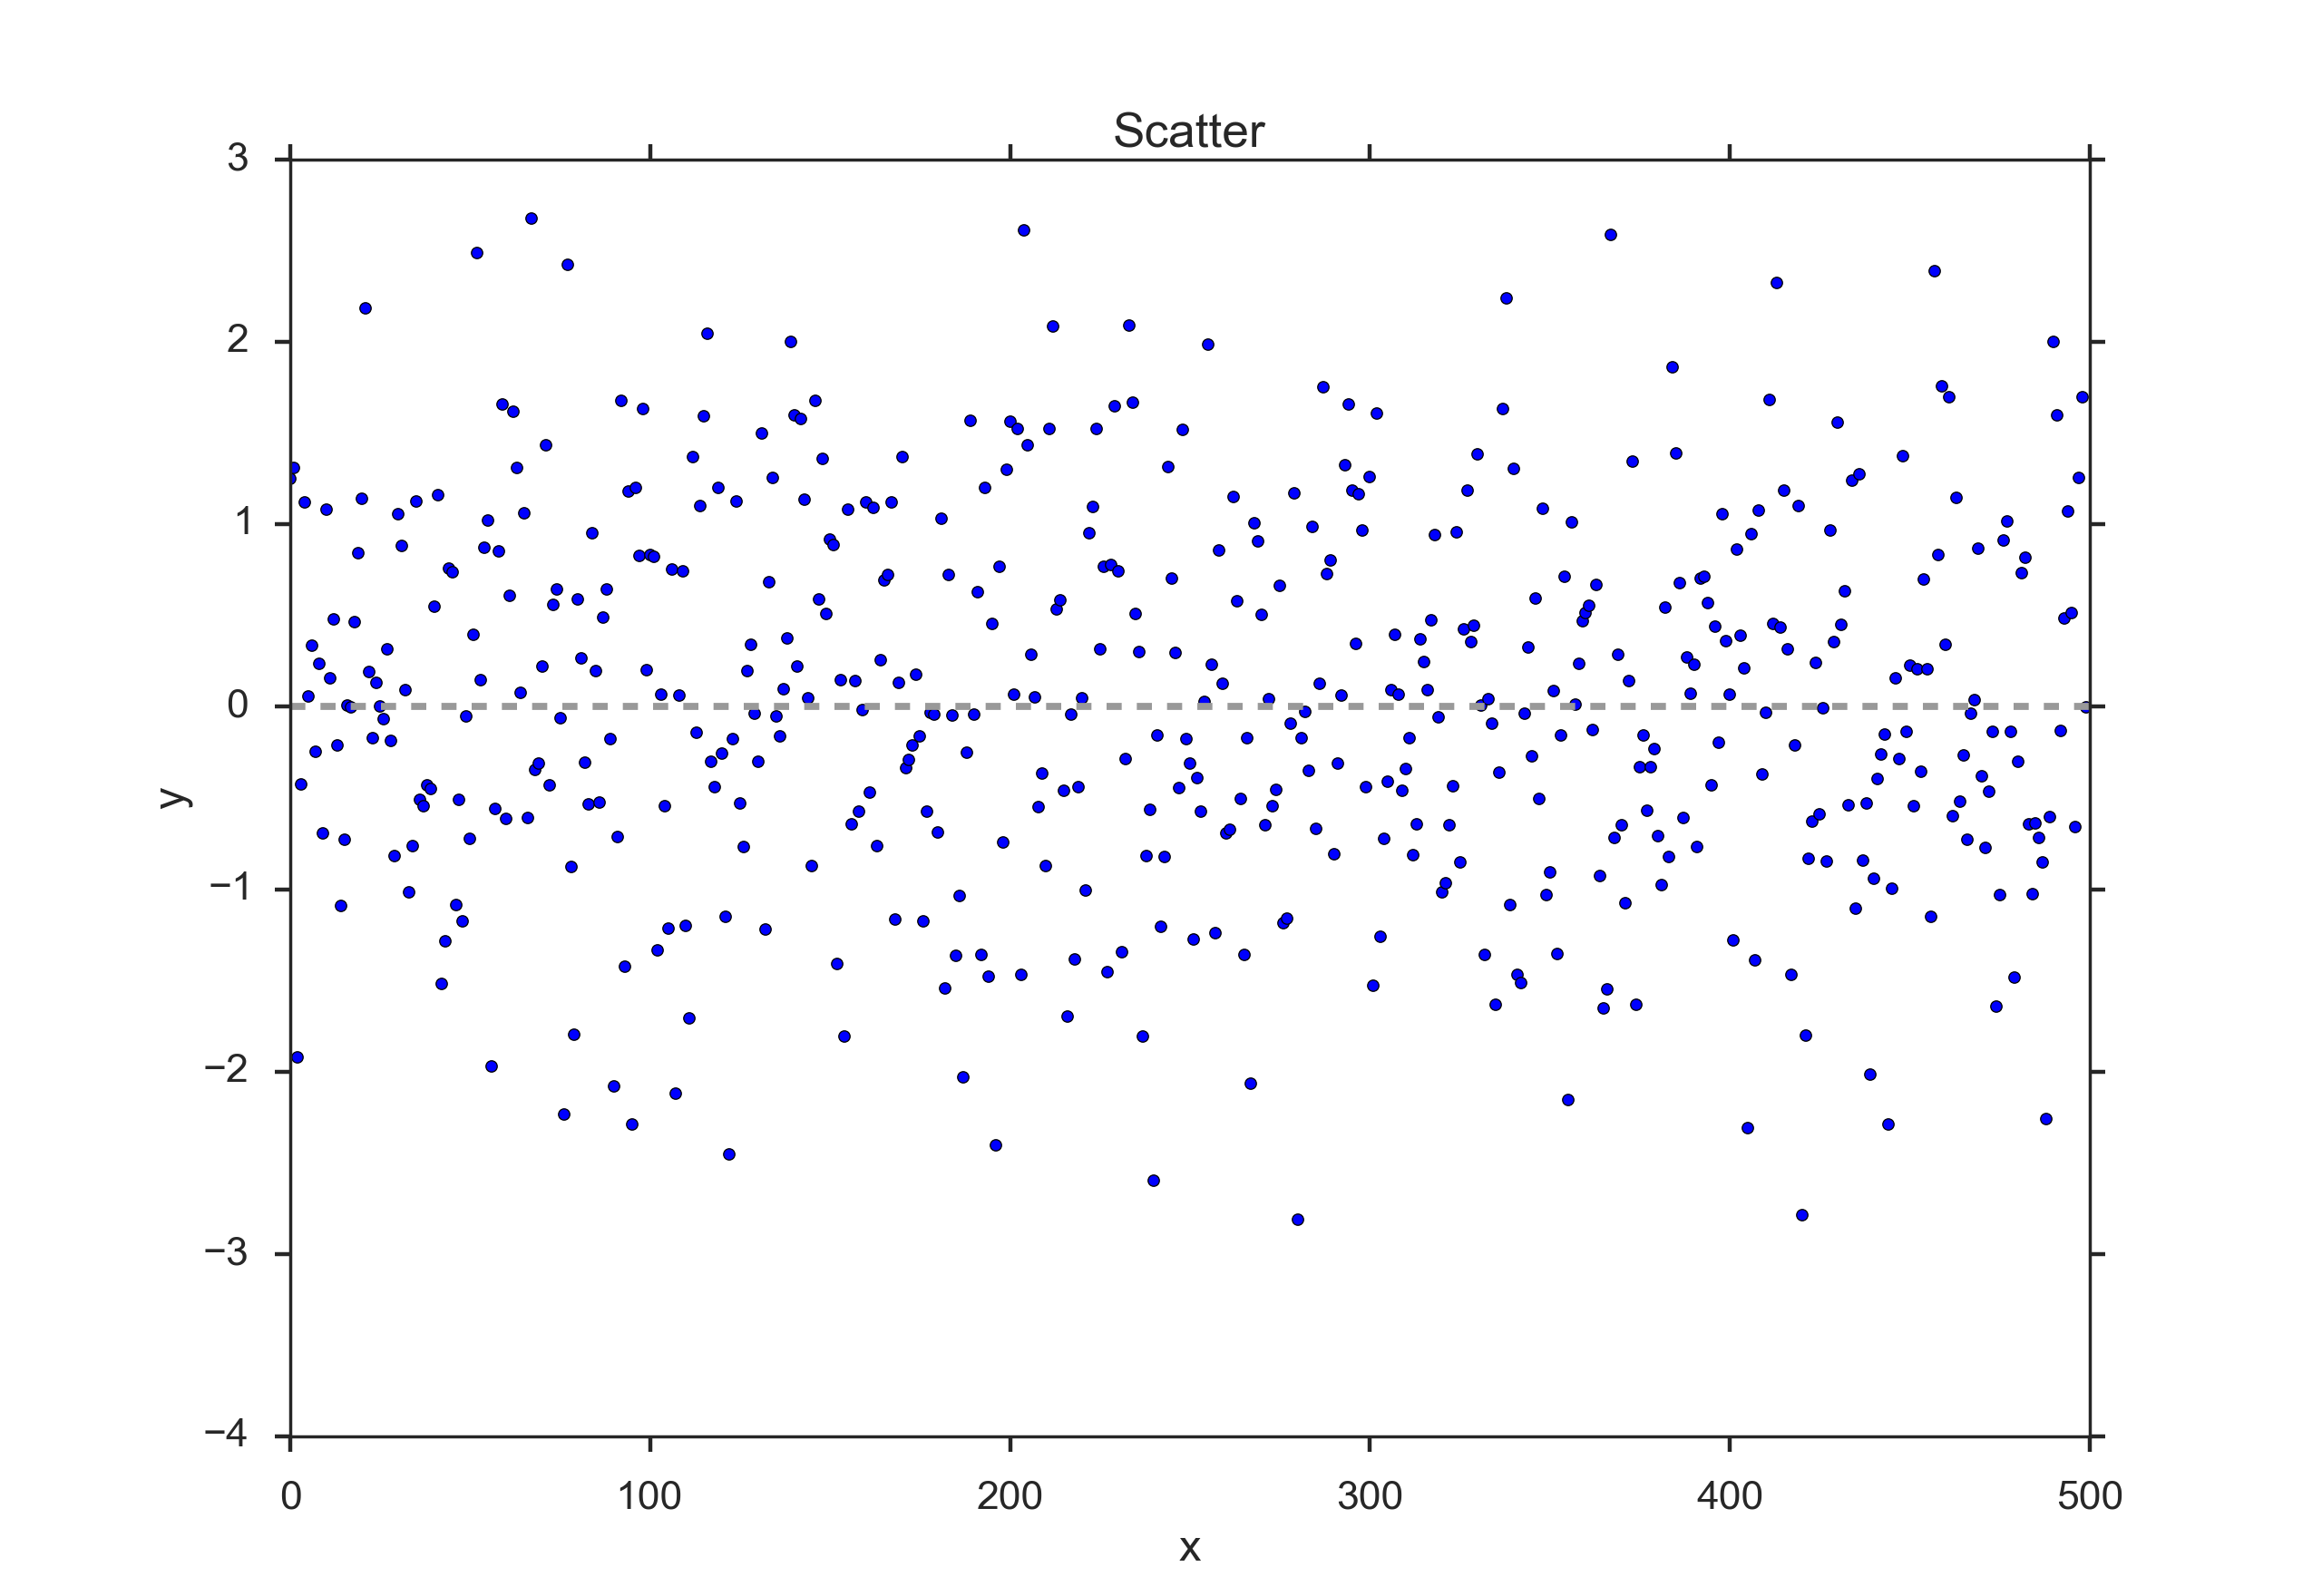
\includegraphics[width=0.5\textwidth]{../Images/scatterPlot.png}\\
  \caption{Scatter plot}
\end{figure}

\subsection{Histograms}\index{general}{plots!histogram}


\emph{Histograms} provide a first good overview of the distribution of your data.
If you divide by the overall number of data points, you get a \emph{relative frequency
histogram}; and if you just connect the top center points of each bin, you obtain a
\emph{relative frequency polygon}.

You can also smooth histograms with \acrfull{kde} (kde-plots). Those are nicely implemented and described in \emph{seaborn}.

\begin{figure}[ht]
  \centering
  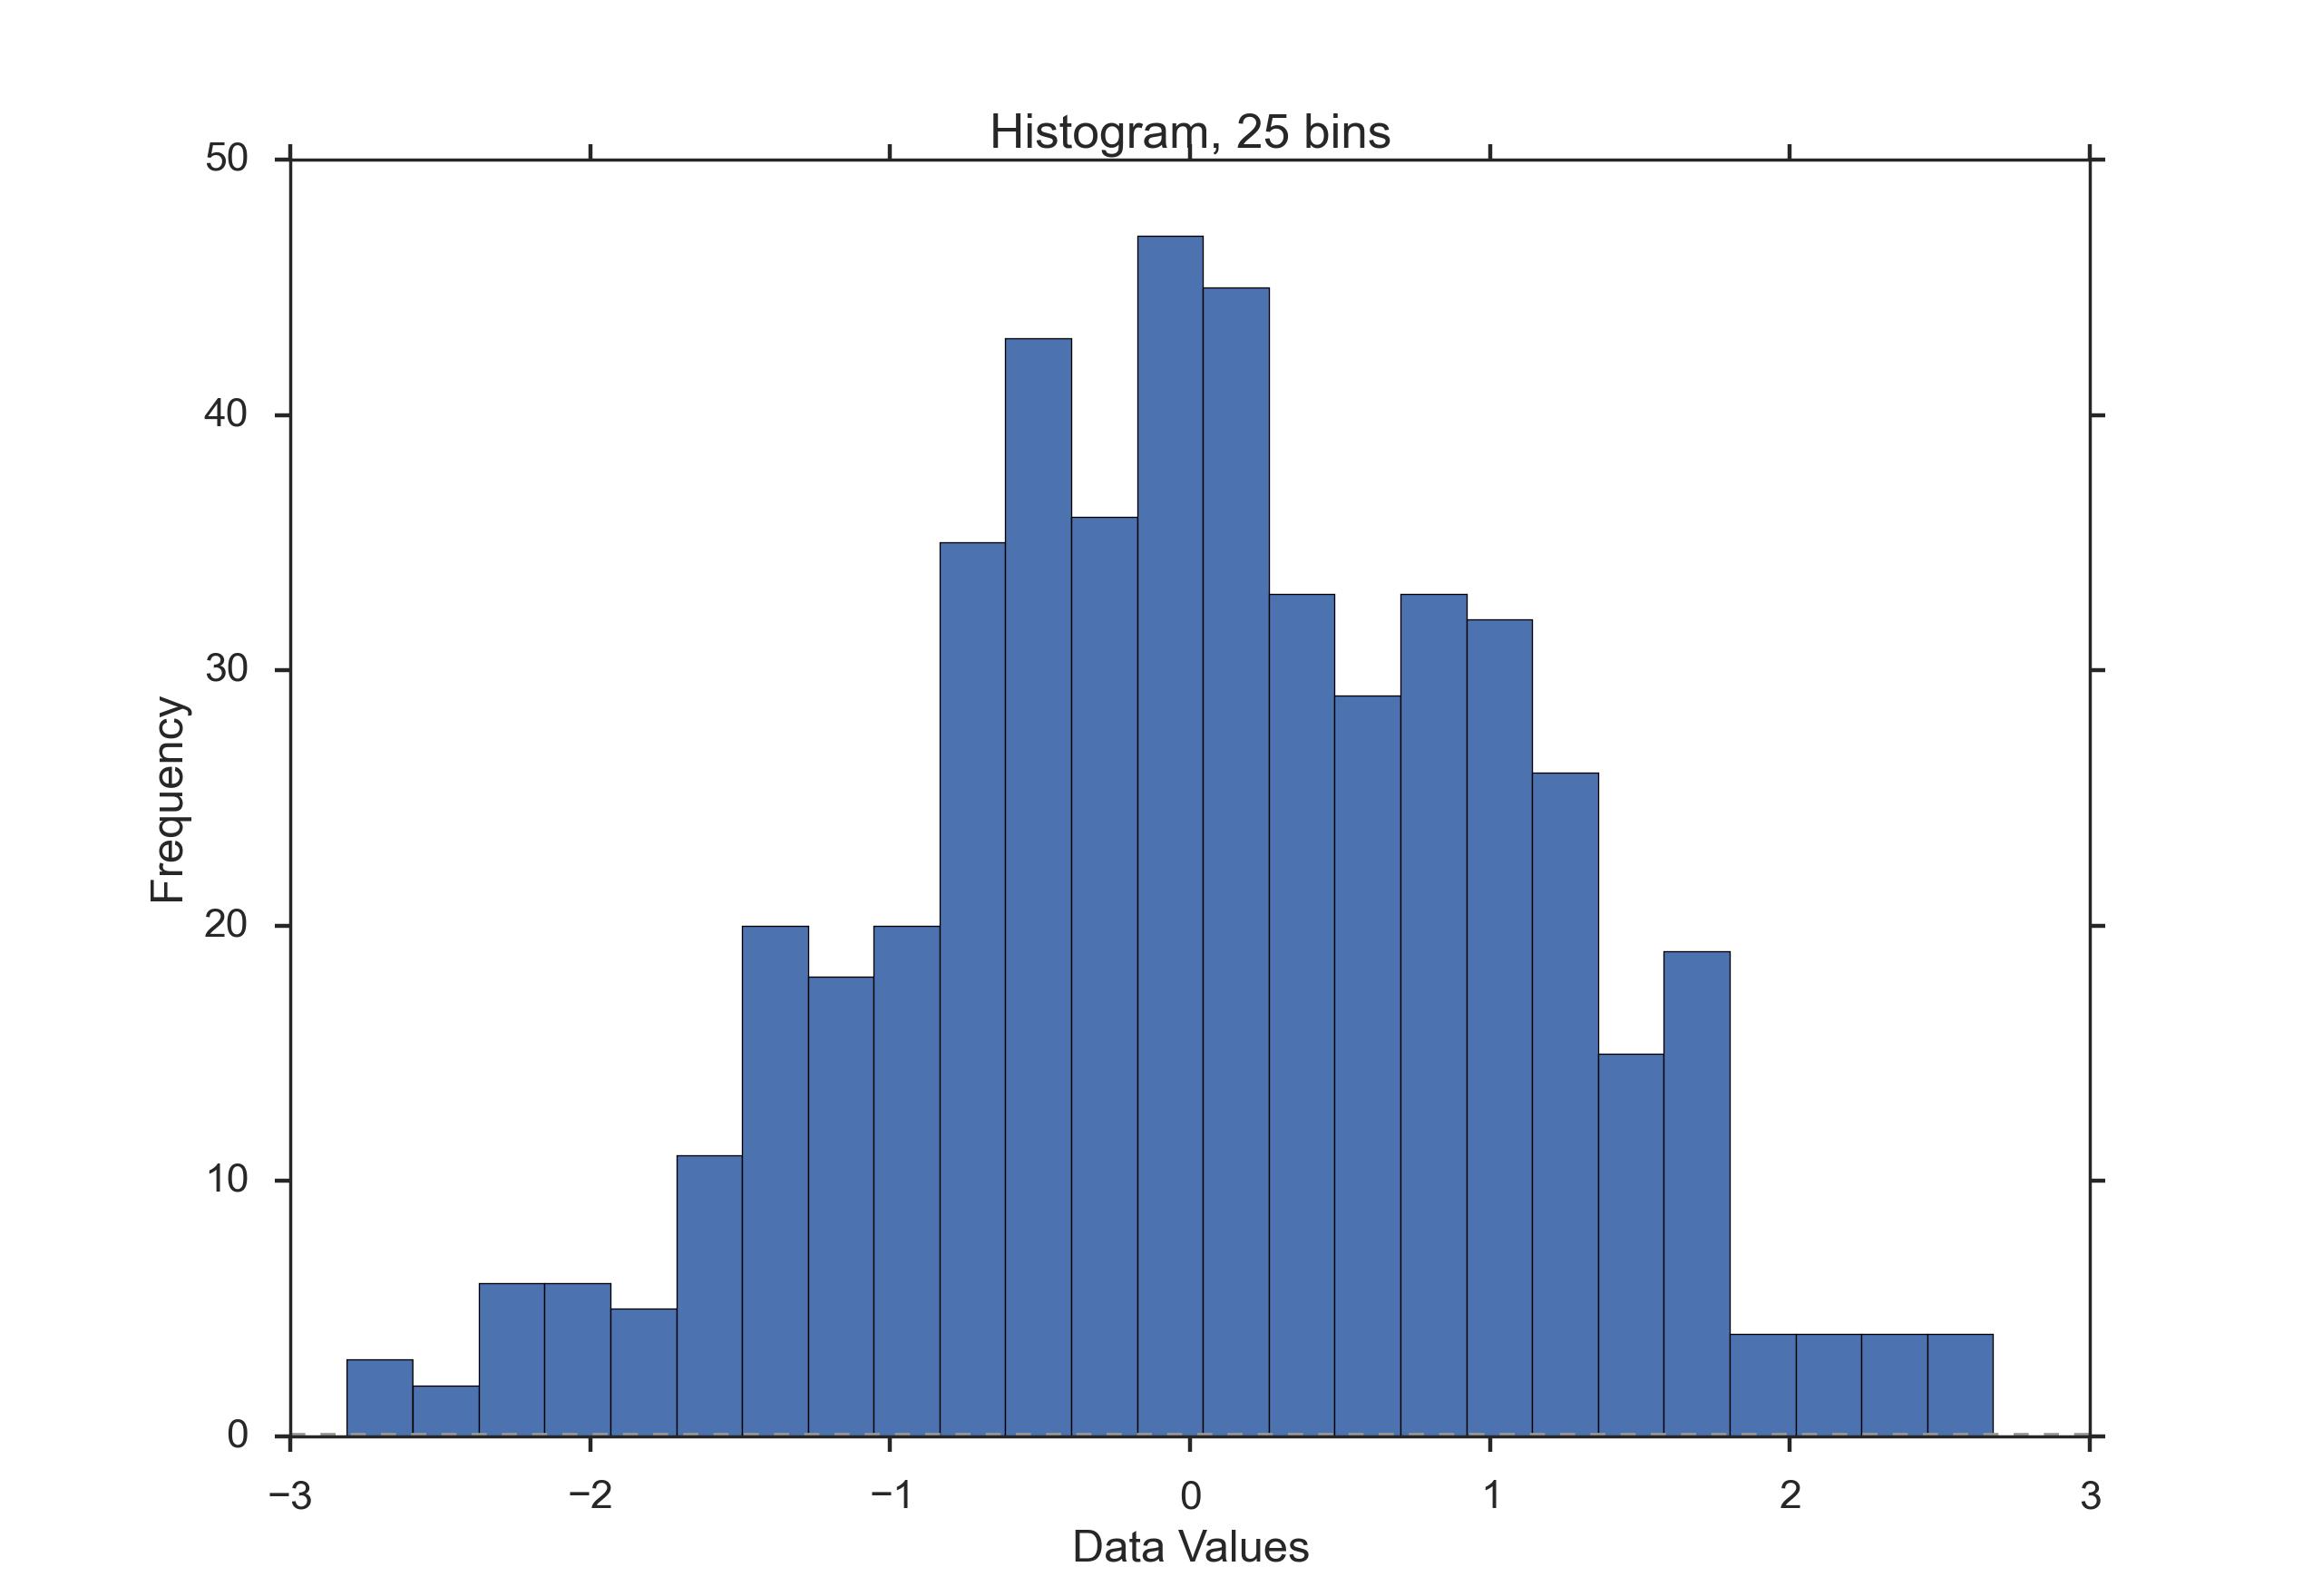
\includegraphics[width=0.5\textwidth]{../Images/Histogram.png}\\
  \caption{Histogram}
\end{figure}

\subsection{KDE-plots}\index{general}{plots!kde}

Histograms have the disadvantage that they are discontinuous, and that their shape critically depends on the chosen bin-width. In order to obtain smooth \emph{probability densities}, i.e. curves describing the likelihood of finding an event in any given interval, the technique of \emph{Kernel \gls{density} Estimation (KDE)}\index{general}{Kernel Density Estimator (KDE)} can be used. Thereby a normal distribution is typically used for the kernel. The width of this kernel function determines the amount of smoothing. To see how this works, we compare the construction of histogram and kernel density estimators, using these 6 data points: x = [−2.1, −1.3, −0.4, 1.9, 5.1, 6.2]. For the histogram, first the horizontal axis is divided into sub-intervals or bins which cover the range of the data. In this case, we have 6 bins each of width 2. Whenever a data point falls inside this interval, we place a box of height 1/12. If more than one data point falls inside the same bin, we stack the boxes on top of each other.

For the kernel density estimate, we place a normal kernel with variance 2.25 (indicated by the red dashed lines) on each of the data points xi. The kernels are summed to make the kernel density estimate (solid blue curve). The smoothness of the kernel density estimate is evident. Compared to the discreteness of the histogram, the kernel density estimates converge faster to the true underlying density for continuous random variables.

\begin{figure}[ht]
  \centering
  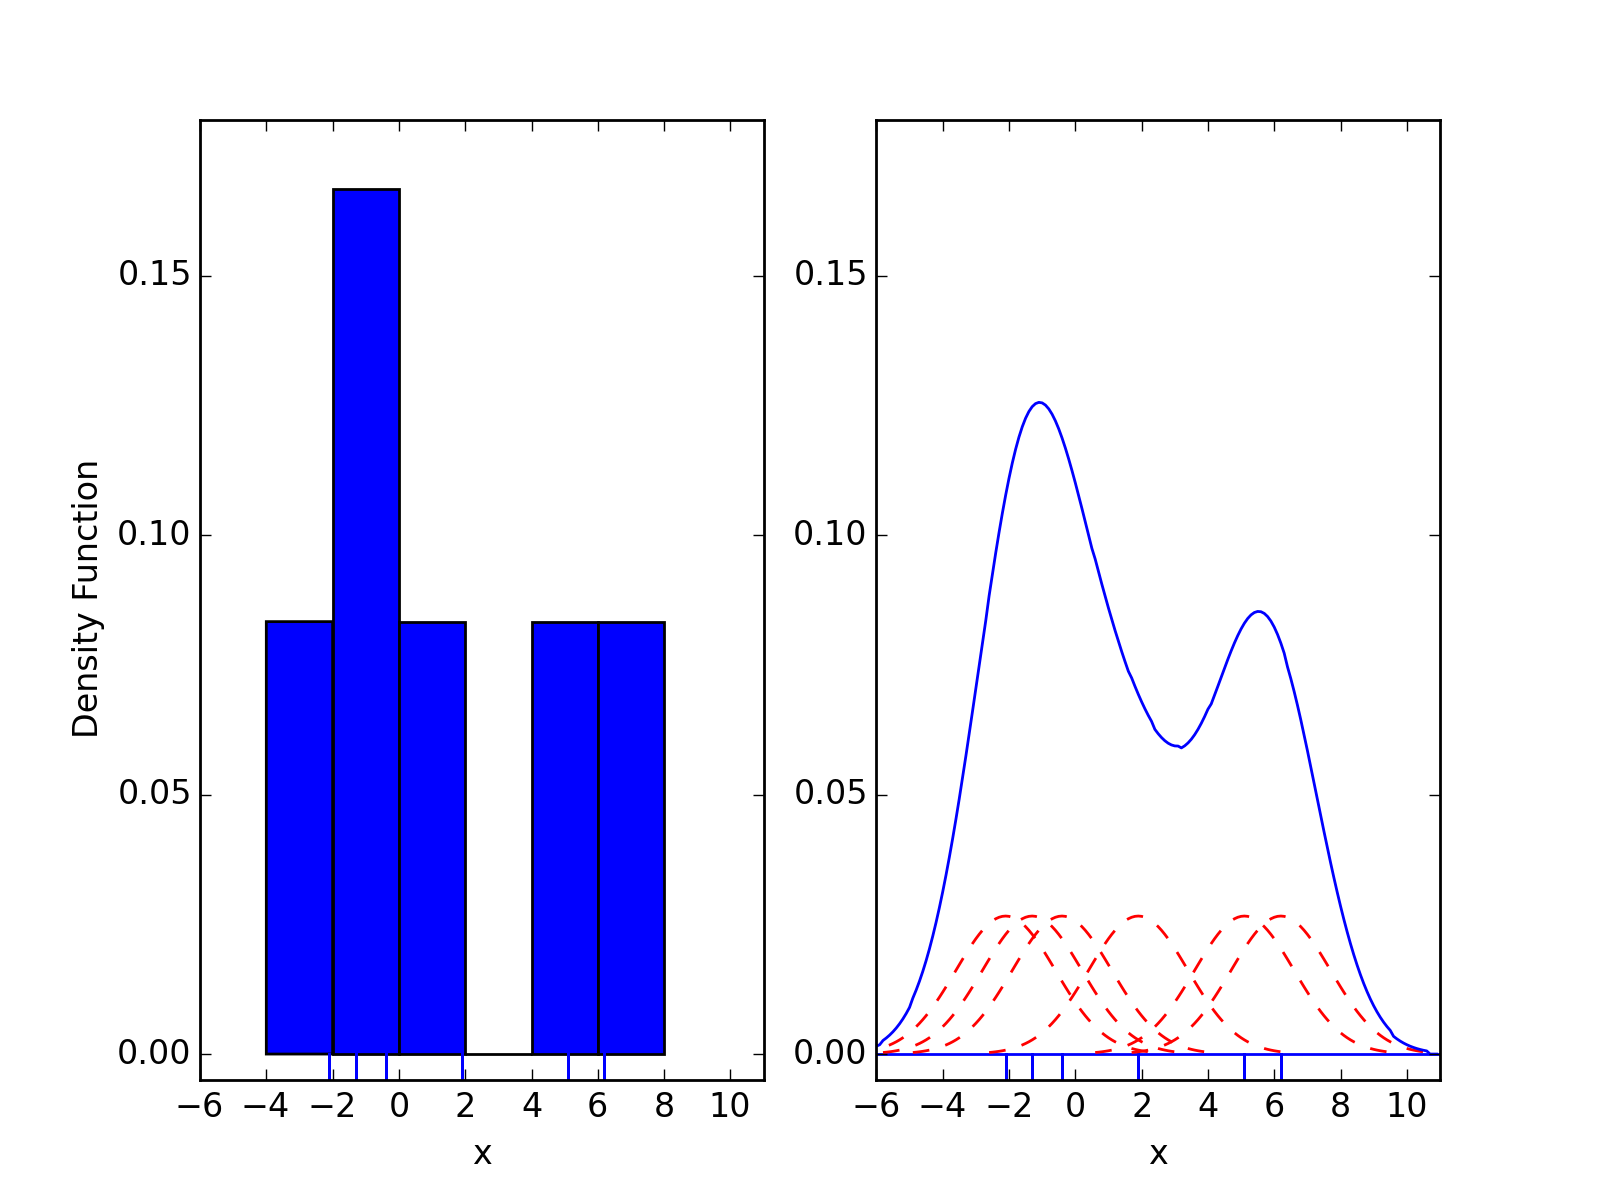
\includegraphics[width=0.75\textwidth]{../Images/KDEexplained.png}\\
  \caption{Comparison of the histogram (left) and kernel density estimate (right) constructed using the same data. The 6 individual kernels are the red dashed curves, the kernel density estimate the blue curves. The data points are the rug plot on the horizontal axis.}
\end{figure}


The bandwidth of the kernel is the parameter which determines how much we smooth out the contribution from each event. To illustrate its effect, we take a simulated random sample from the standard normal distribution, plotted as the blue spikes in the rug plot on the horizontal axis in Fig. \ref{fig:kdeBandwidth}, left. The right plot shows the true density (blue. a normal density with mean 0 and variance 1). In comparison, the gray dashed curve is undersmoothed since it contains too many spurious data artifacts arising from using a bandwidth h = 0.1 which is too small. The green dashed curve is oversmoothed since using the bandwidth h = 1 obscures much of the underlying structure. The red curve with a bandwidth of h = 0.42 is considered to be optimally smoothed since its density estimate is close to the true density.

\begin{figure}[ht]
  \centering
  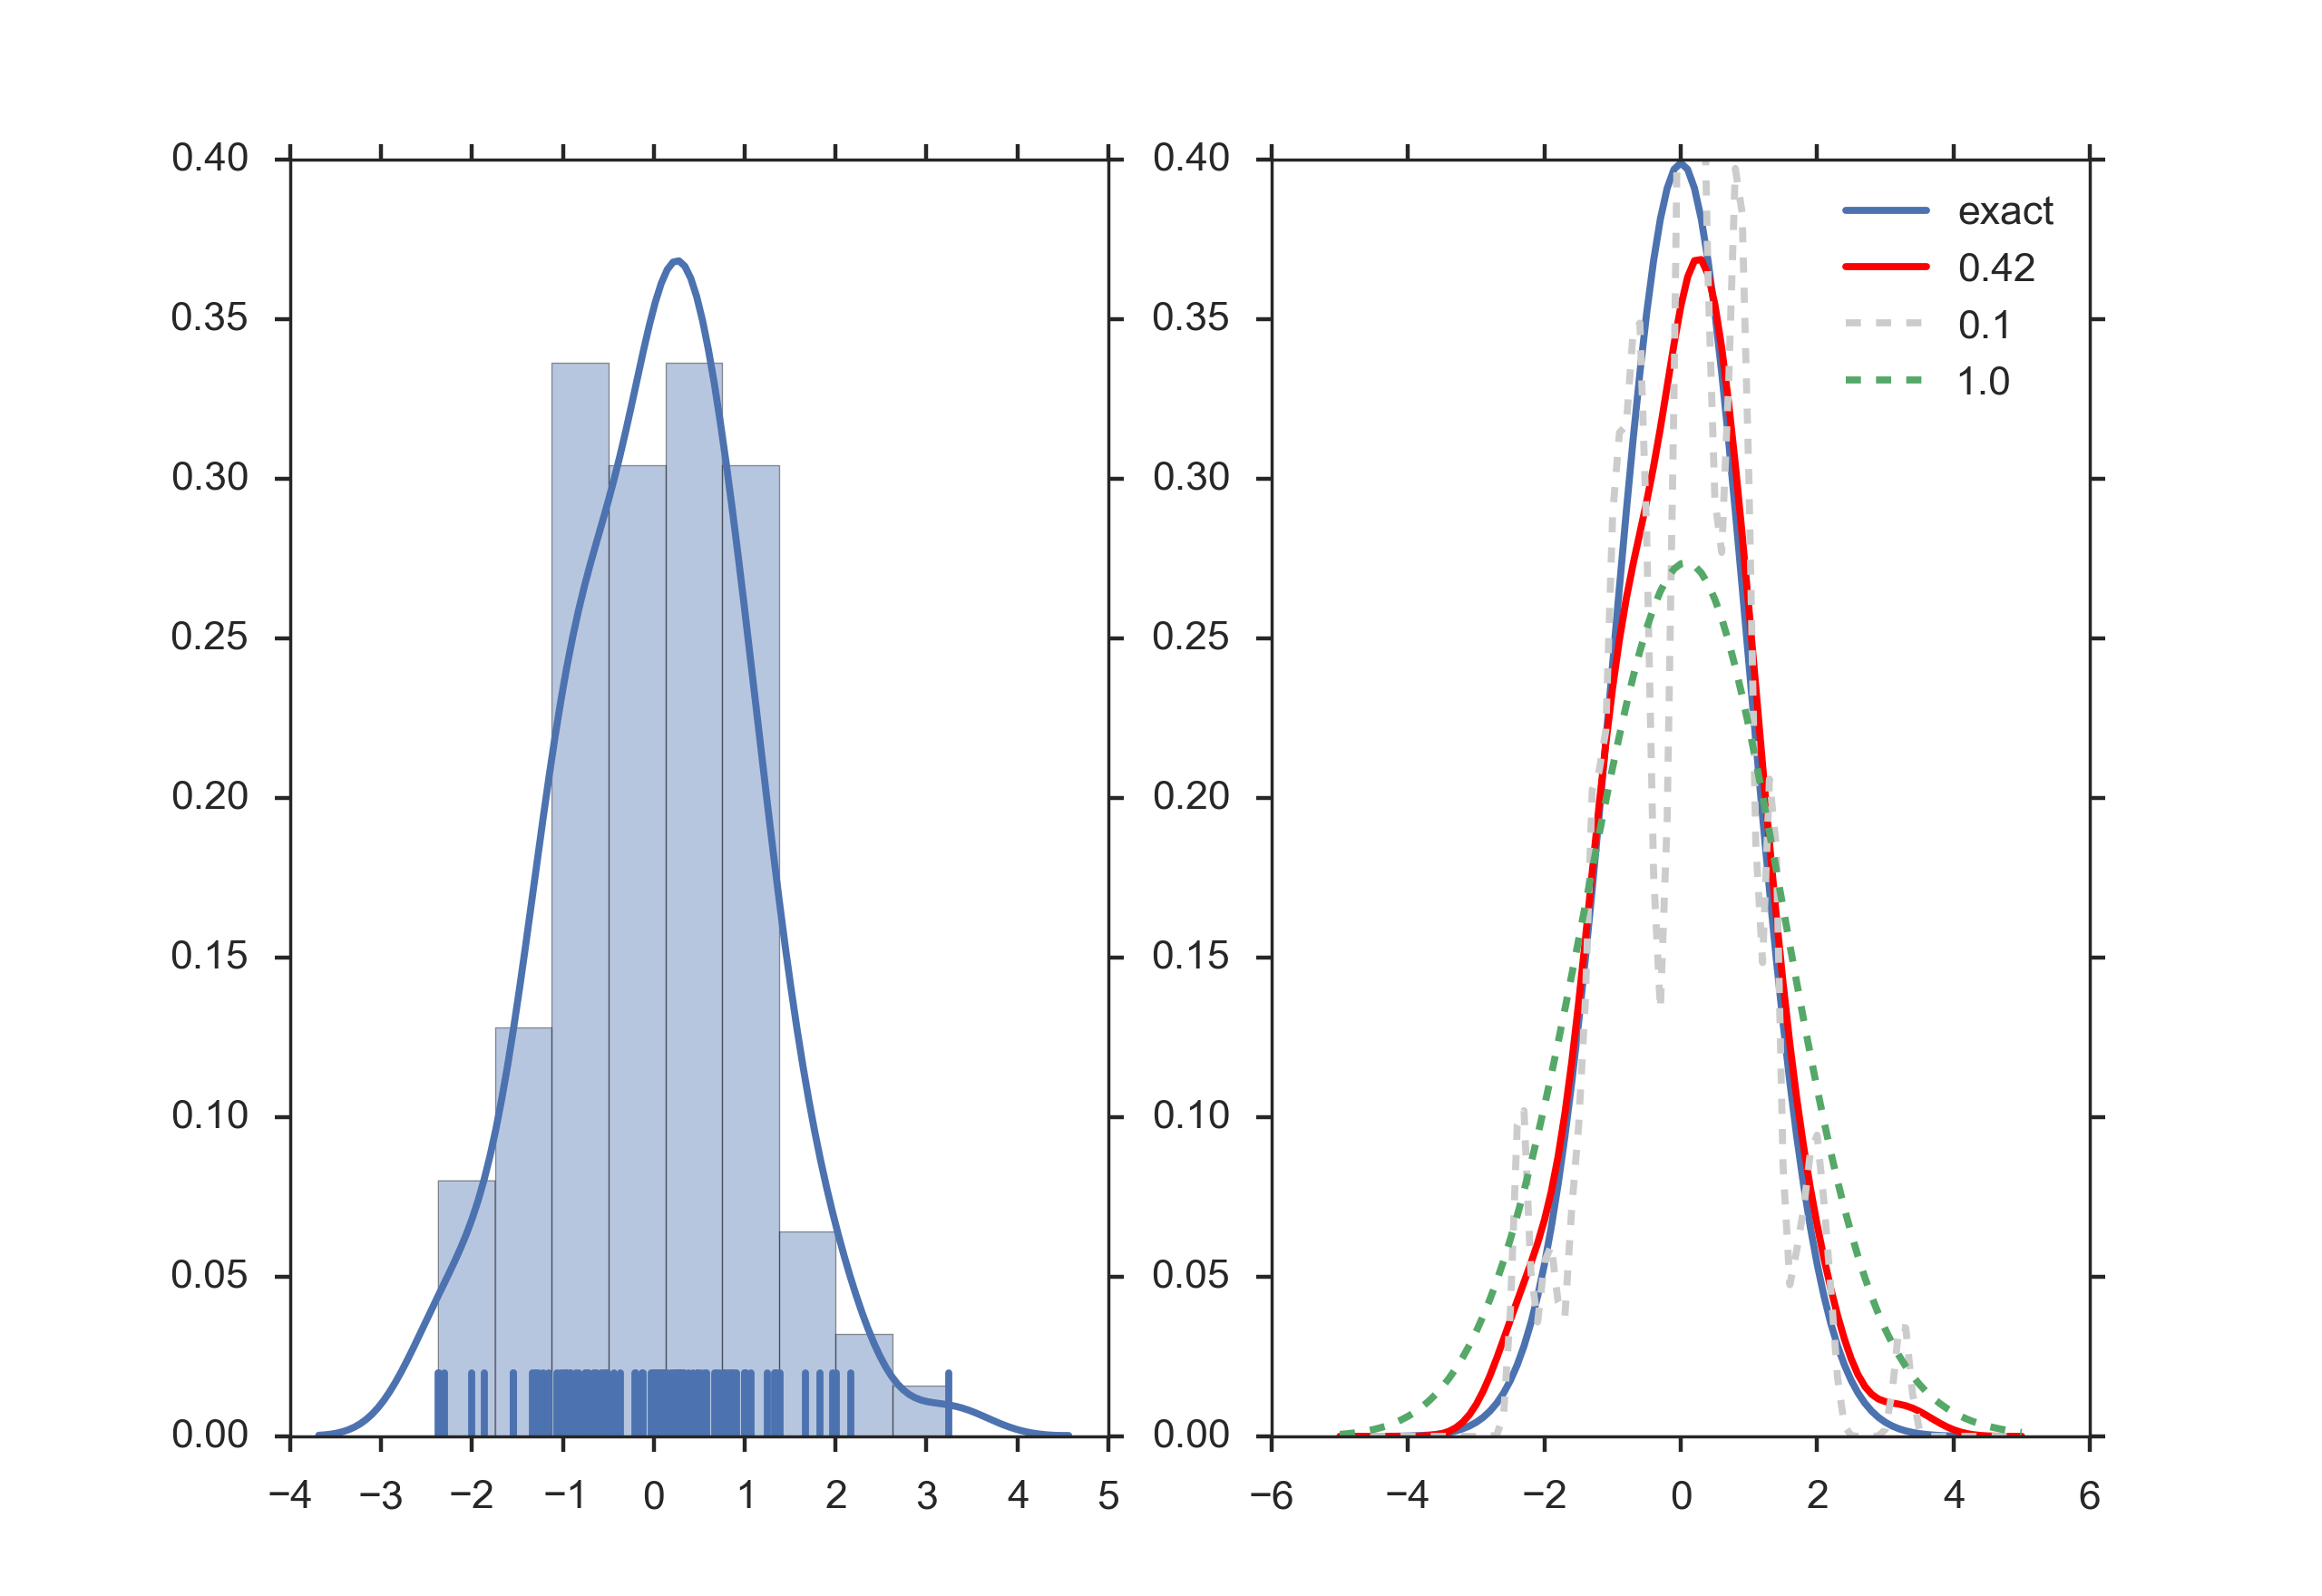
\includegraphics[width=0.75\textwidth]{../Images/KDEplot.png}\\
  \caption{ Left: Rug plot, histogram, and Kernel density estimate (KDE) of a random sample of 100 points from a standard normal distribution. Right: True density distribution (blue), and KDE with different bandwidths. Gray dashed: KDE with h=0.1; red: KDE with h=0.42 green dashed: KDE with h=1.0.}
  \label{fig:kdeBandwidth}
\end{figure}

It can be shown that under certain conditions the optimal choice for h is

\begin{equation}
  h = \left(\frac{4\hat{\sigma}^5}{3n}\right)^{\frac{1}{5}} \approx 1.06 \hat{\sigma} n^{-1/5},
\end{equation}

where $\hat{\sigma}$ is the standard deviation of the samples ("Silverman's rule of thumb").

\subsection{Cumulative Frequencies}\index{general}{cumulative frequency}

\emph{Cumulative frequency} curves indicate the number (or percent) of data with less than a given value. This is important for the statistical analysis (e.g. when we want to know the data range containing 95\% of all the values). Cumulative frequencies
are also useful for comparing the distribution of values in two or more different groups of individuals.

When you use percentage points, the cumulative frequency presentation has the additional advantage that it is bounded:

\begin{equation*}
  0 \leq x \leq 1
\end{equation*}

\begin{figure}[ht]
  \centering
  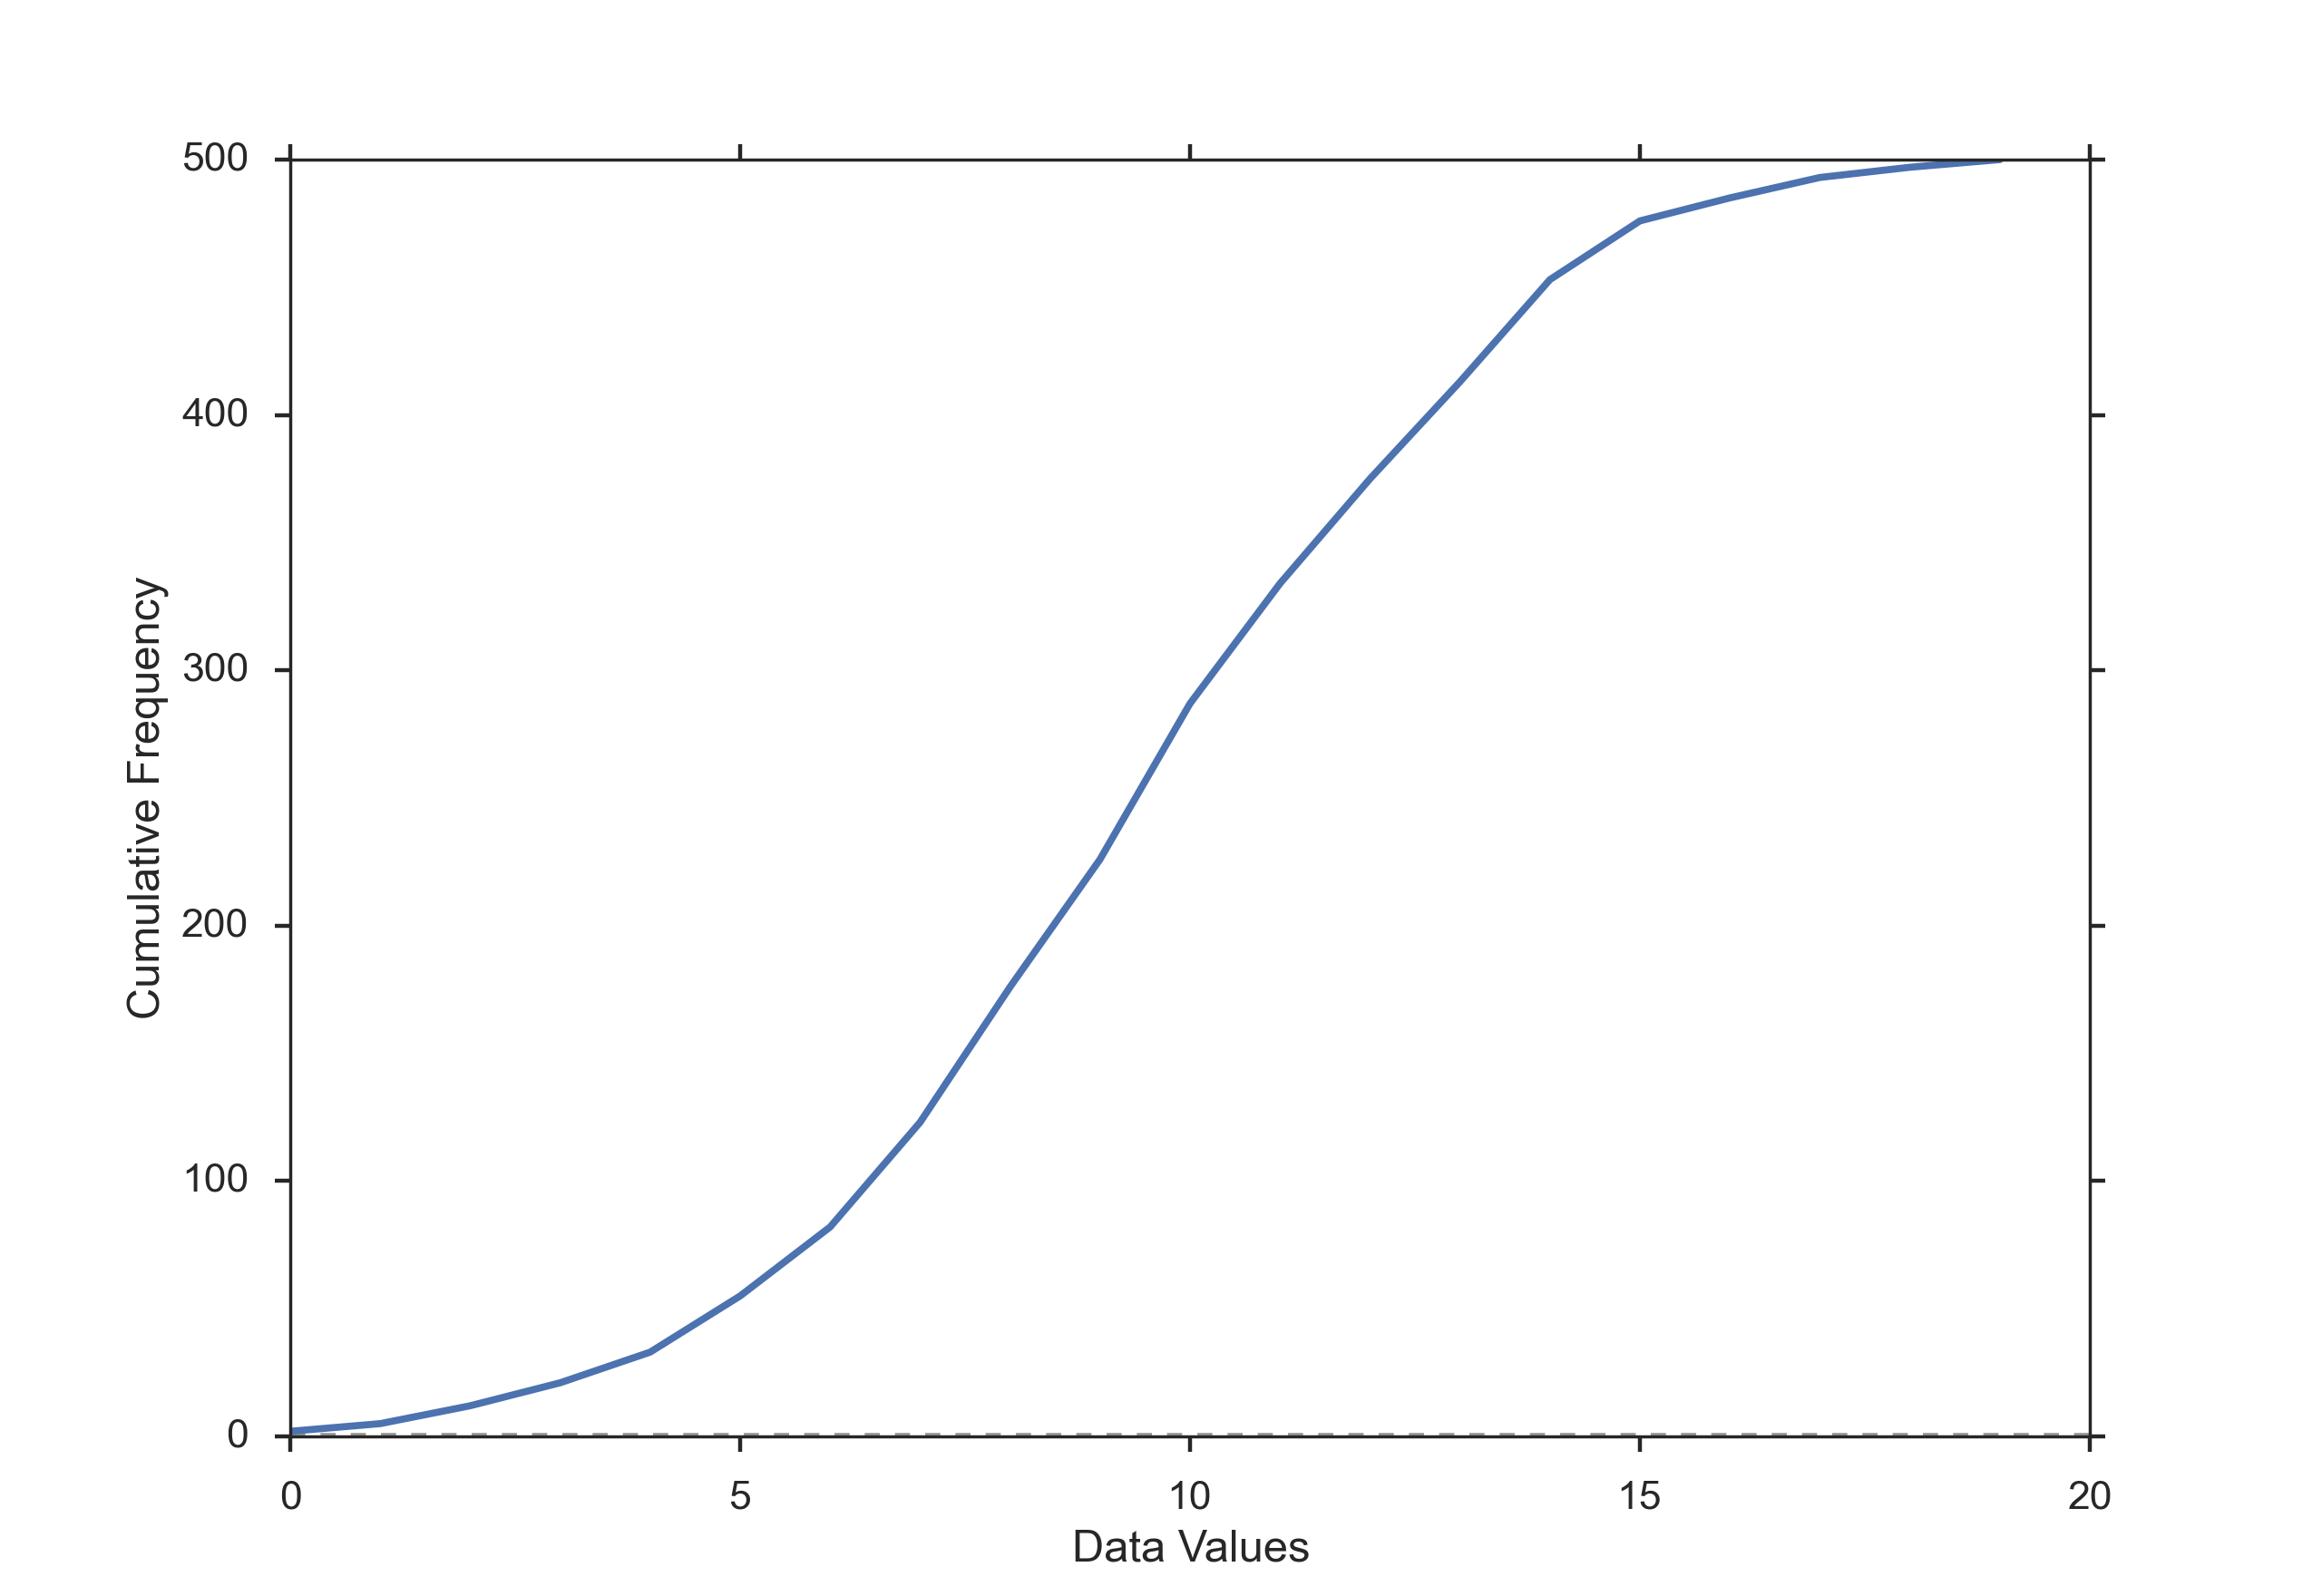
\includegraphics[width=0.5\textwidth]{../Images/CumulativeFrequencyFunction.png}\\
  \caption{Cumulative frequency function for a normal distribution.}
\end{figure}

\subsection{Errorbars}\index{general}{plots!errorbars}

\emph{Errorbars} are a common way to show mean value and variability when comparing a few measurement values. Note that you have to state explicitly if your errorbars correspond to the \emph{standard devation} or to the \emph{standard error} of the data. Using \emph{standard errors} has a nice feature: When error bars for the \emph{standard error} for two groups overlap, you can be sure the difference between the two means is not statistically significant (P>0.05). Watch out, though, since the opposite is not always true!

\begin{figure}[ht]
  \centering
  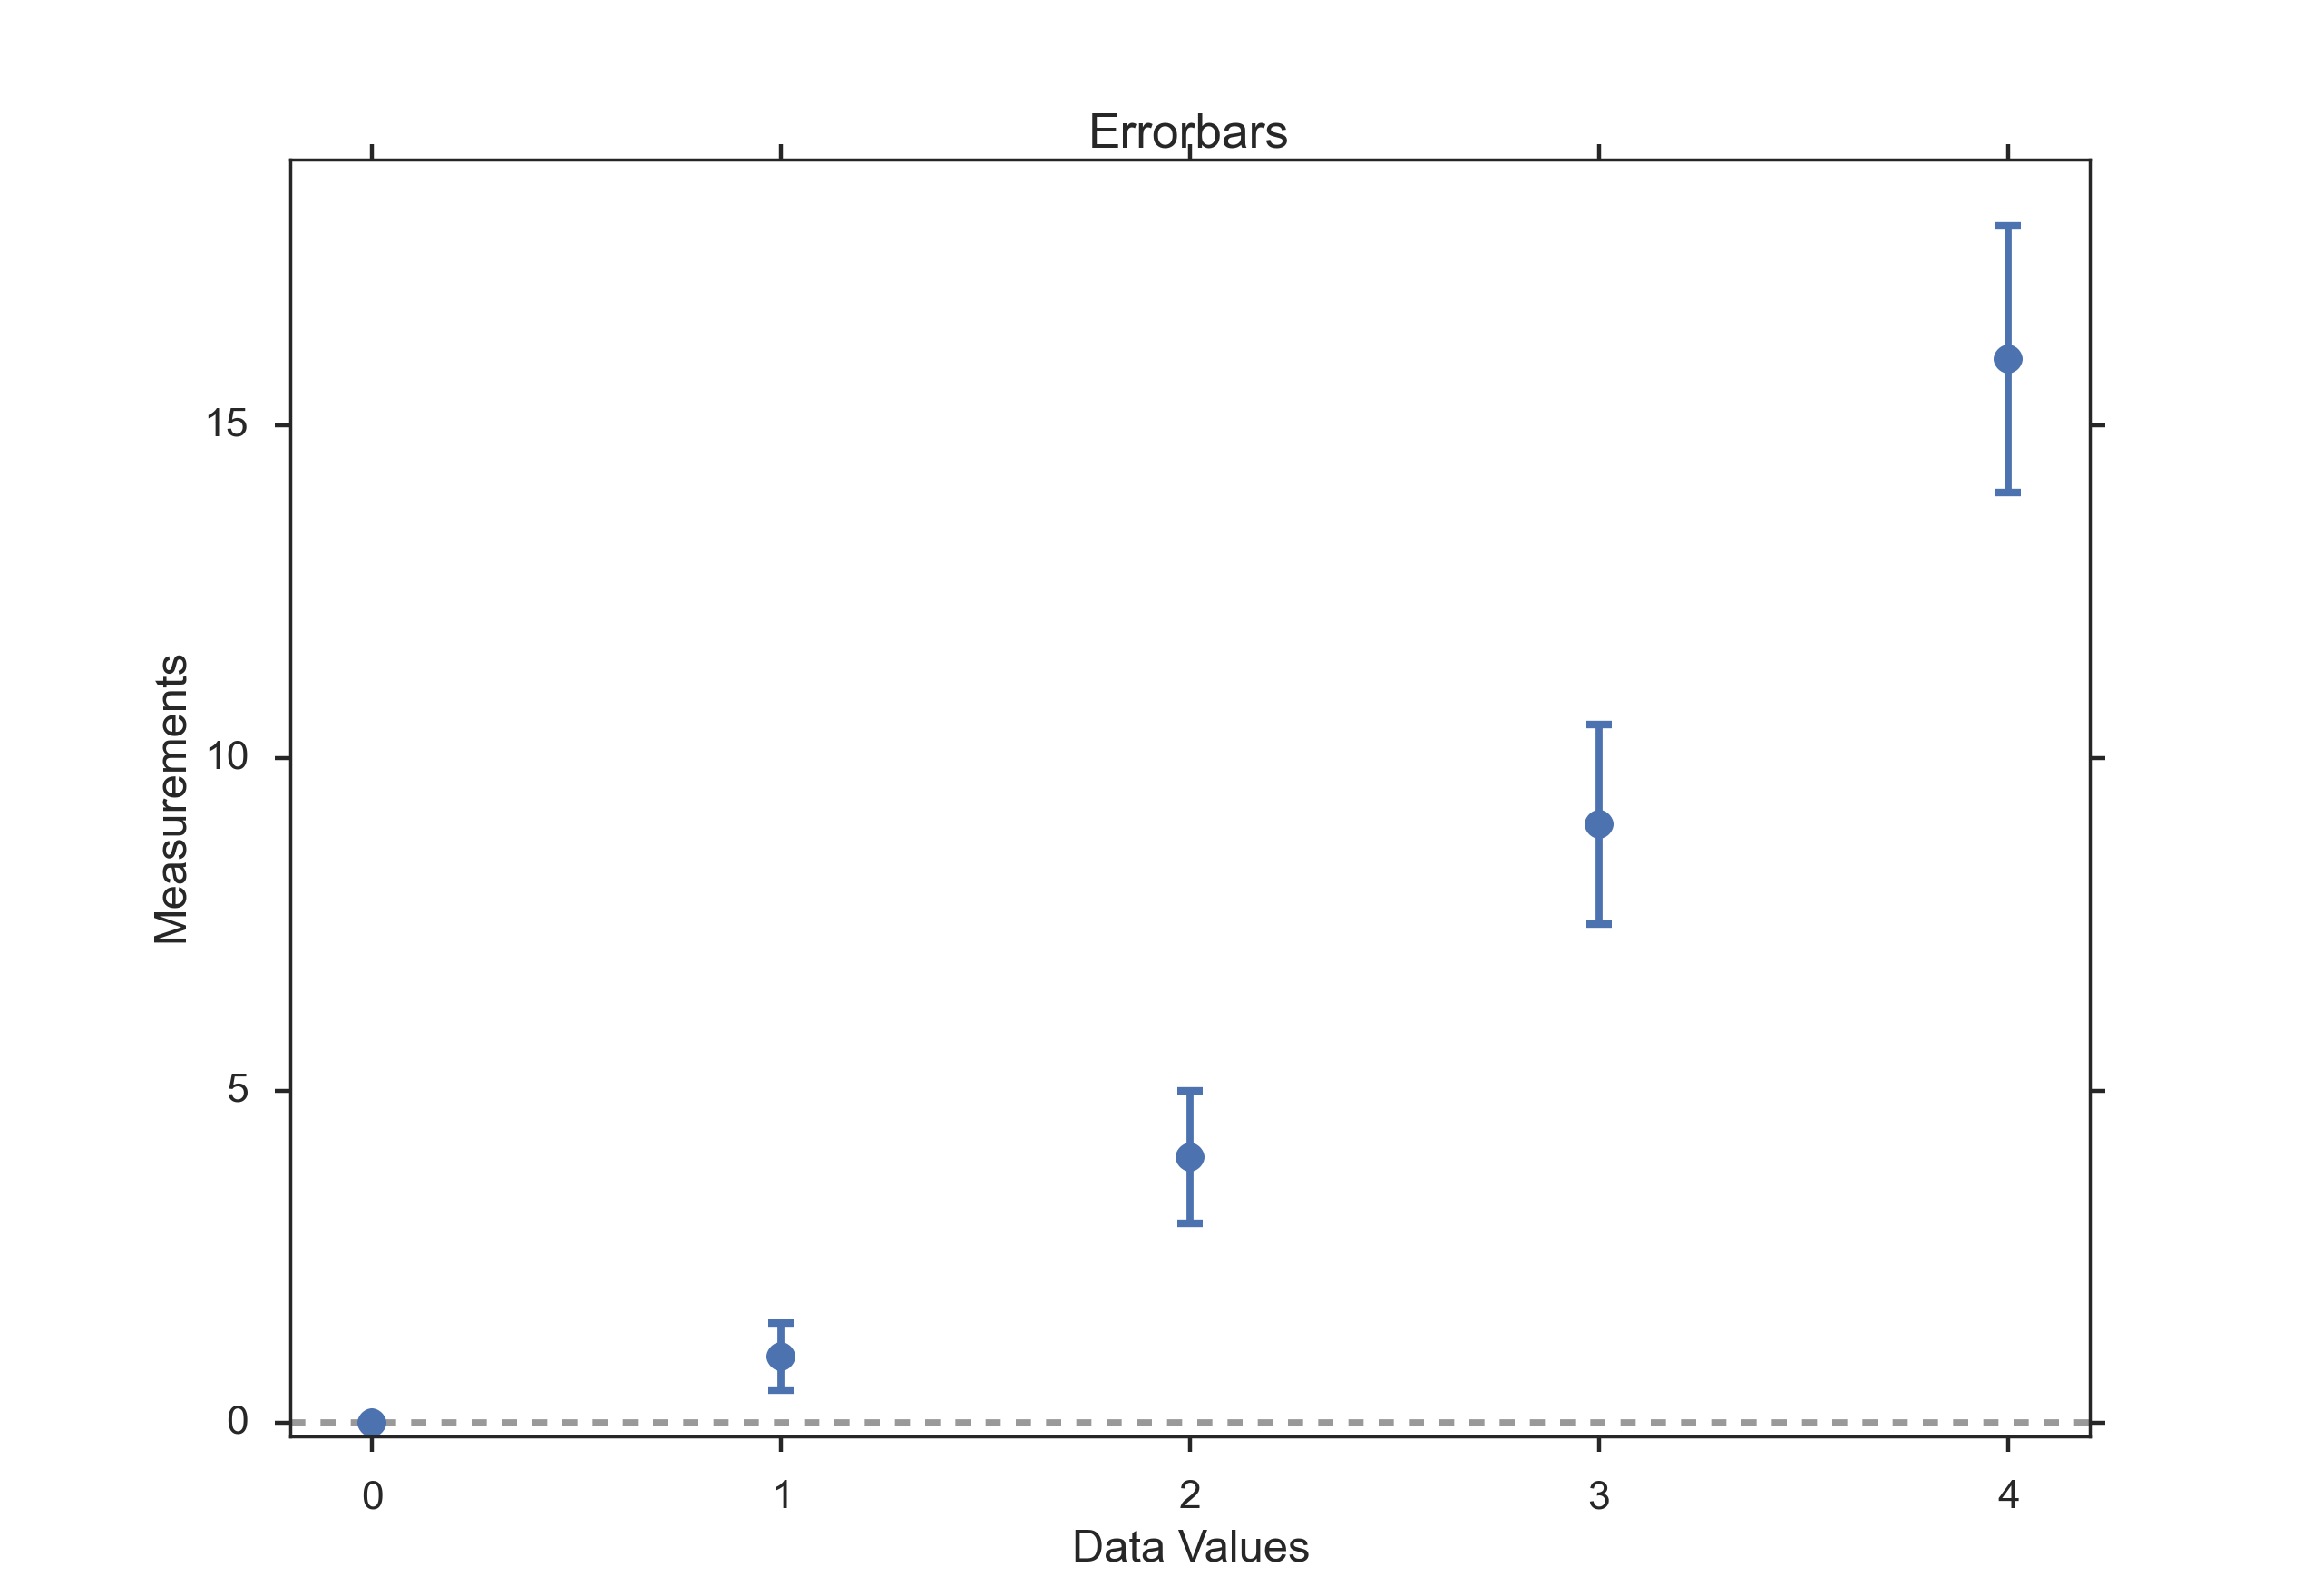
\includegraphics[width=0.5\textwidth]{../Images/Errorbars.png}\\
  \caption{Errorbars}
\end{figure}


\subsection{Box Plots}\index{general}{plots!boxplot}

\Glspl{boxplot} are frequently used in scientific publications to indicate values in two or more groups. The bottom and top of the box indicate the first and third \glspl{quartile}, and the line inside the box shows the median. Care has to be taken with the whiskers, as different conventions exist for them. The most common form is that the lower whisker indicates the lowest value still within 1.5 \emph{inter-quartile-range} (IQR)\index{general}{inter-quartile-range, IQR} of the lower quartile, and the upper whisker the highest value still within 1.5 IQR of the upper quartile. Outliers (outside the whiskers) are plotted separately. Another convention is to have the whiskers indicate the full data range.

There are a number of tests to check for outliers\index{general}{outliers}. The method suggested by Tukey is to check for data which lie more than 1.5 * IQR above or below the first/third quartile (see Section \ref{sec:centiles}).

\begin{figure}[!ht]
  \centering
  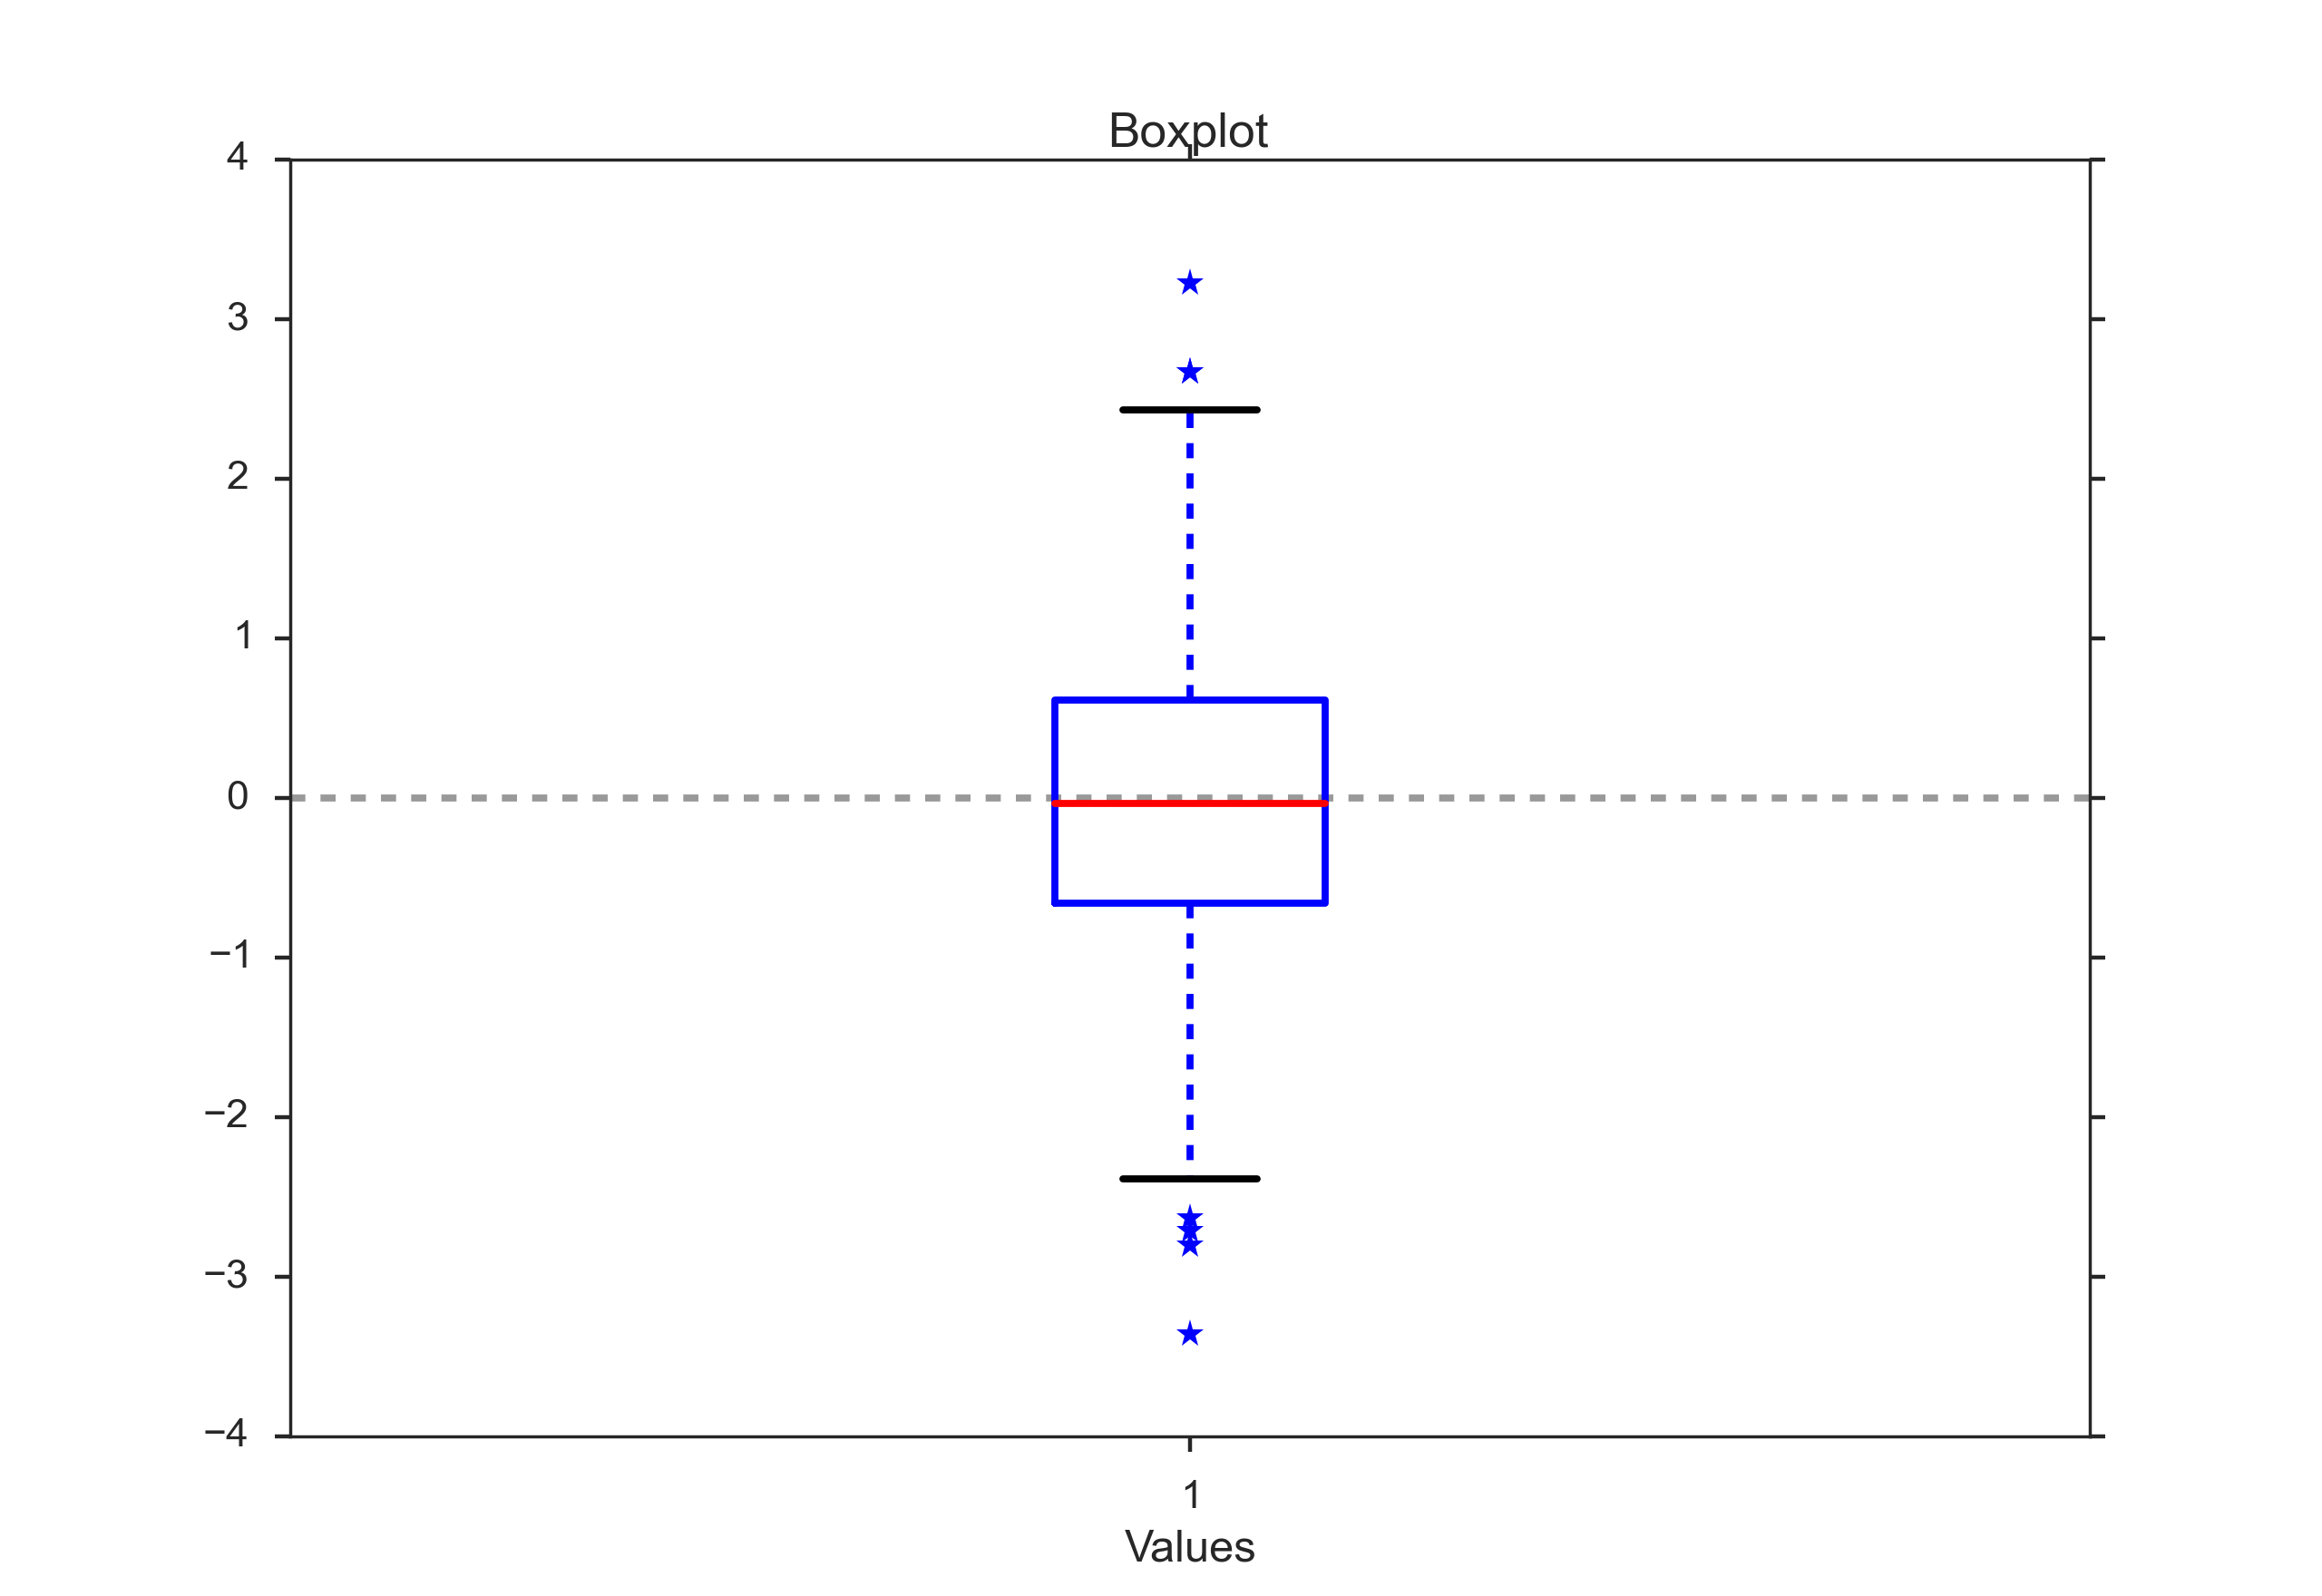
\includegraphics[width=0.5\textwidth]{../Images/boxplot.png}\\
  \caption{Box plot}\label{fig:Boxplot}
\end{figure}

Boxplots are often combined with KDE-plots to produce so-called \emph{violin-plots} \index {general}{plots!violinplot}, as shown in Figure \ref{fig:violin}.

\begin{figure}
  \centering
  % Requires \usepackage{graphicx}
  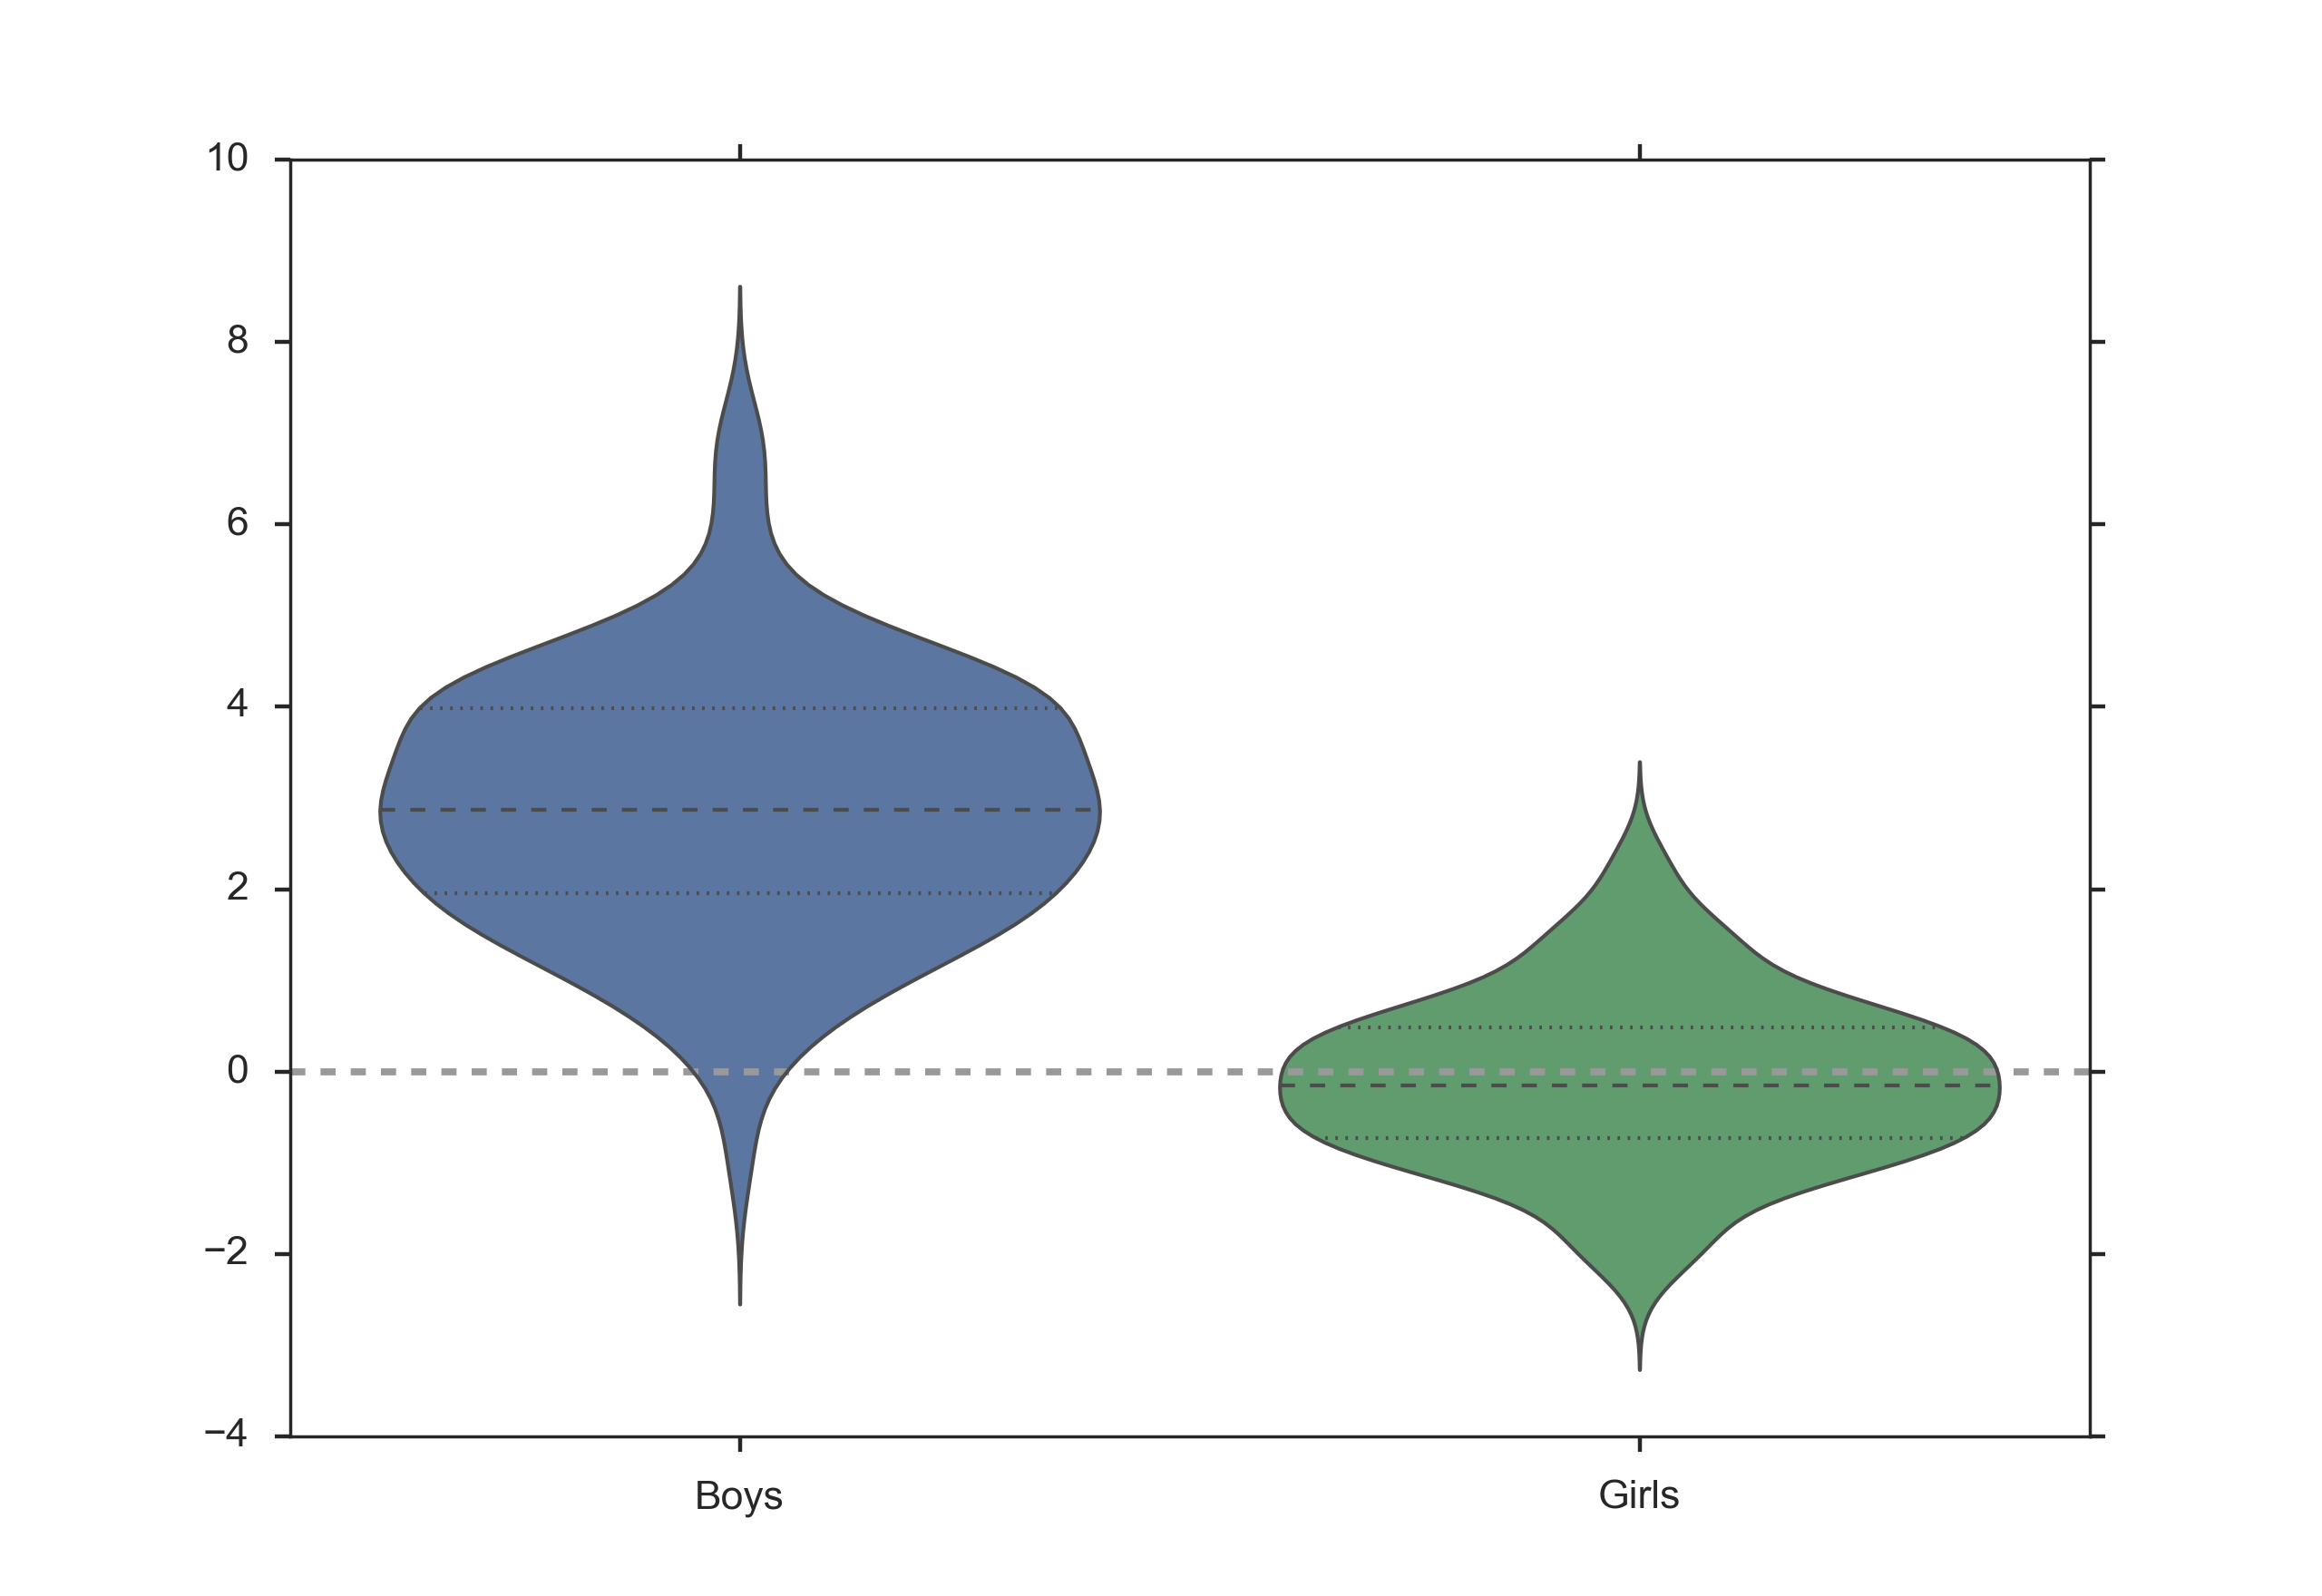
\includegraphics[width=0.75\textwidth]{../Images/violinplot.png}\\
  \caption{Violinplot, produced with \emph{seaborn}.}\label{fig:violin}
\end{figure}

\subsection{Programs: Data Display}
\PyImg "figsBasicPrinciples.py" (p \pageref{py:BasicPrinciples}) shows how the plots in this section have been generated.
\index{python}{figsBasicPrinciples}

\section{Populations and Samples}

The main difference between a \gls{population}\index{general}{population} and a \gls{sample}\index{general}{sample} has to do with how observations are assigned to the data set (see Fig. \ref{fig:population}).

\begin{description}
  \item[Population] includes all of the elements from a set of data.
  \item[Sample] consists of one or more observations from the population.
\end{description}

\begin{figure}
  \centering
  % Requires \usepackage{graphicx}
  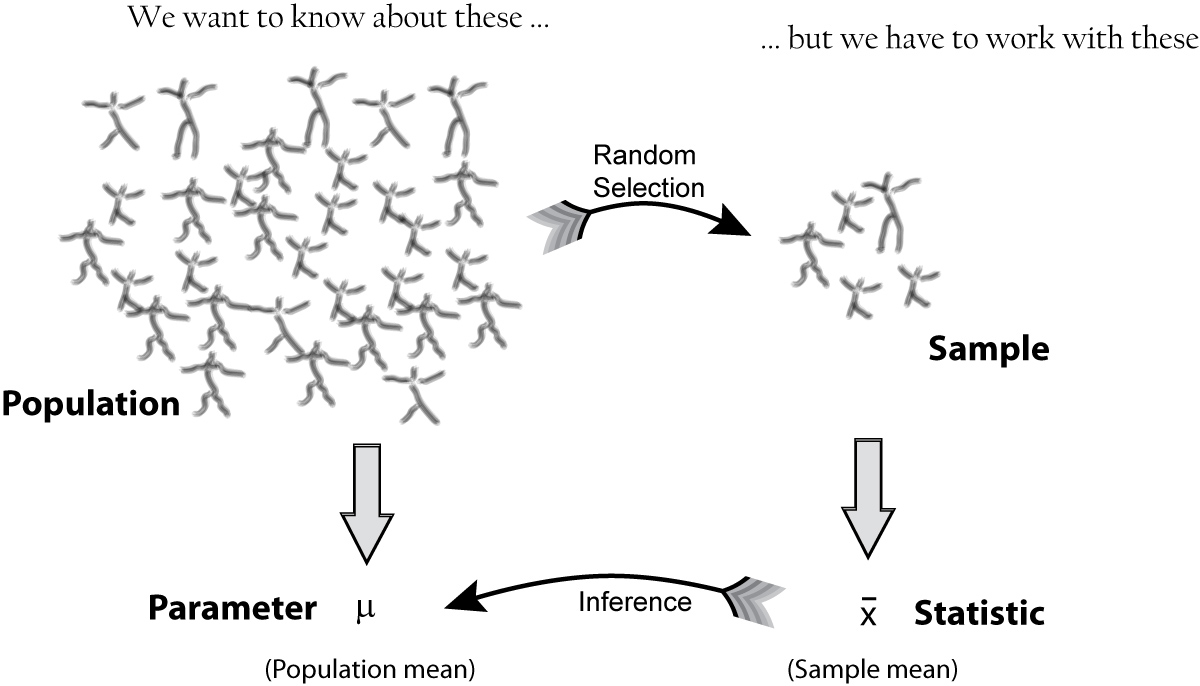
\includegraphics[width=1.0\textwidth]{../Images/PopulationAndSample.jpg}\\
  \caption{With statistical inference information from Samples is used to estimate Parameters from Populations.}\label{fig:population}
\end{figure}

More than one sample can be derived from the same population.

When estimating a \emph{parameter} of a \emph{population}, e.g. the weight of male Europeans, we can typically never measure all of them. We have to confine ourselves to investigate a (hopefully representative) random \emph{sample} of this group. Based on the \emph{sample statistic}, we use \emph{statistical inference}\index{general}{inference} to find out what we know about the \emph{parameter}.

\begin{description}
  \item[Parameter] characteristic of a population, such as a mean or standard deviation. Often denoted with Greek symbols.
  \item[Statistic] a measurable characteristic of a sample.
  \item[Sampling distribution] is the probability distribution of a given statistic based on a random sample.
  \item[Statistical inference] enables you to make an educated guess about a population parameter based on a statistic computed from a sample randomly drawn from that population.
\end{description}

An example for parameters and statistics is given in Table \ref{table:population}.

\begin{table}[ht]

  \centering
    \begin{tabular}{|l|c|c|}
      \hline
       & Sample Statistic & Population Parameter \\
       \hline
      Mean & $\bar{x}$ & $\mu$ \\
      Standard Deviation & s & $\sigma$ \\
      \hline
    \end{tabular}
    \caption{Comparison of Sample Statistics and Population Parameters.}
    \label{table:population}
\end{table}

\section{Degrees of Freedom}\label{sec:DF}

The concept of \gls{dof_} \acrshort{dof} \index{general}{degrees of freedom, DOF}, which in mechanics seems to be crystal clear, is harder to grasp for statistical applications.

In mechanics, a particle which moves in a plane has \emph{2 DOF}: at each point in time, two parameters (the x/y-coordinates) define the location of the particle. If the particle moves about in space, it is said to have \emph{3 DOF}: the x/y/z-coordinates.

In statistics, a group of \emph{n} values has \emph{n} DOF. If we only look at the shape of the distribution of the values, we can subtract from each value the sample mean. Then, the remaining data only have \emph{n-1} DF. (This is clearest for $n=2$: if you know the mean value and the value of sample 1, then you can calculate the value of sample 2 by $val_2 = 2*mean - val_1$.

The case becomes more complex if we have many groups. For example, in chapter \ref{sec:anova}, we describe an example with 22 patients, divided into 3 groups. In the \emph{analysis of variance (ANOVA)}, these are divided as follows:

\begin{itemize}
  \item 1 DOF for the total mean value.
  \item 2 DOF for the mean value of each of the three groups (remember, if we know the mean values of 2 groups \emph{and} the total mean, we can calculate the mean value of the third group.
  \item 19 DOF are left for the residuals.
\end{itemize}

\section{Study Design}

\subsection{Terminology}

\begin{figure}
  \centering
  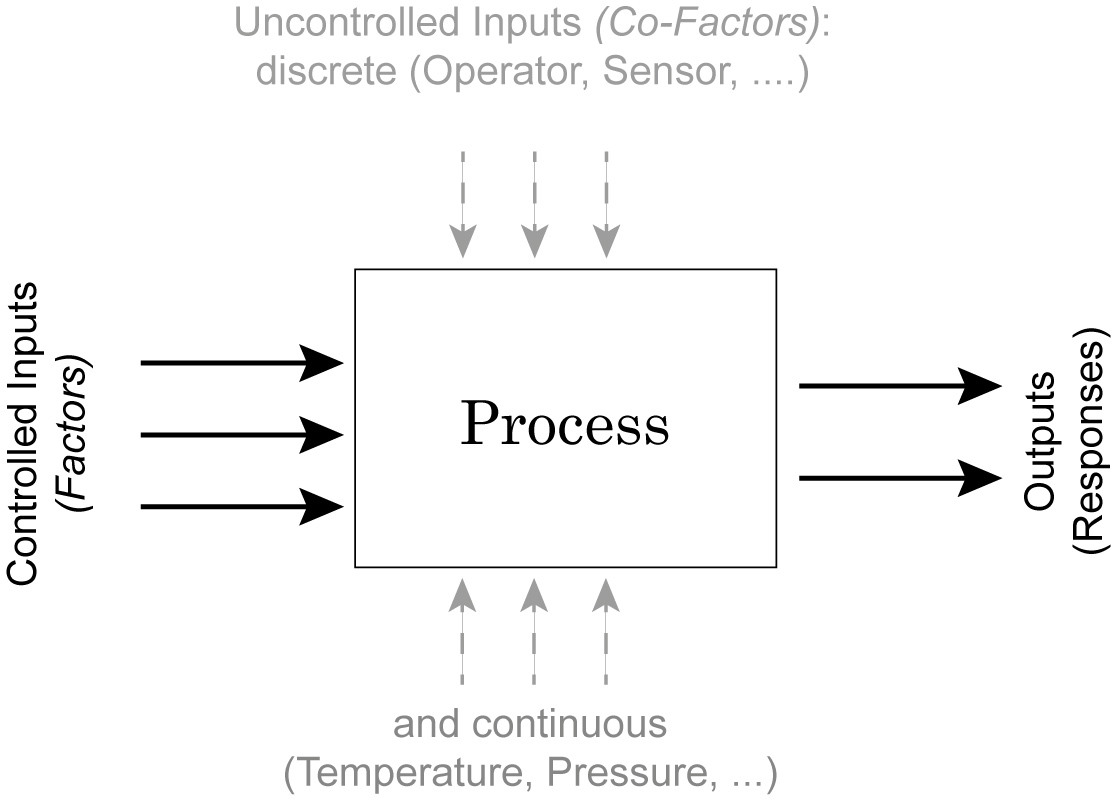
\includegraphics[width=0.75\textwidth]{../Images/Process_Optimization.jpg}\\
  \caption{Process Schematic}\label{fig:StudyDesign}
\end{figure}

In the context of study design, different terminologies can be found (Fig. \ref{fig:StudyDesign}):

\begin{itemize}
    \item{The controlled inputs are often called \glspl{factor}\index{general}{factors} or
            \gls{treatment}\index{general}{treatments}.}
    \item{The uncontrolled inputs are called \emph{co-factors}\index{general}{co-factors} or
            \emph{nuisance factors}.}
\end{itemize}

When we try to model a process with two inputs and one outputs, we can
formulate a mathematical model for example as

\begin{equation}
    X = \beta_0 + \beta_1 X_1 + \beta_2 X_2 + \beta_{12} X_1 X_2 + \epsilon
\end{equation}

The terms with the single "X's" are called \emph{main effects}\index{general}{main effects}, and the terms with multiple "X's" \emph{interaction terms}\index{general}{interactions}. And since the $\beta$
parameters enter the equation only linearly, this is referred to as a \emph{general linear model}. The $\epsilon$s are called \glspl{residual}\index{general}{residuals}, and are expected to be approximately normally distributed around zero.

\subsection{Overview}

The first question you have to ask yourself is what you want to do. Do you want to

\begin{itemize}
    \item{Compare two or more groups, or one group to a fixed value?}
    \item{Screen the observed responses to identify
            factors/effects that are important?}
    \item{Maximize or minimize a response (variability, distanct to target,
            robustness)?, or}
    \item{Develop a regression model to quantify the dependence of a
            response variable on the process input?}
\end{itemize}

The first question leads to an \gls{hypothesistest}. The second one is a screening investigation, where you have to watch out for \emph{multiple testing artefacts}. The third task is an optimization problem. And the last one brings you into the realm of \emph{statistical modeling}.

Once you have determined \emph{what} you want to do, you have to decide \emph{how} you want to do this. You can either do \emph{controlled experiments}. Or you can use \emph{observations} to obtain the data that you are looking for. In a controlled experiment you typically try to vary only a single parameter, and investigate the effects of that parameter on the output.

\subsection{Personal Tips}

\begin{enumerate}
  \item Be realistic about your task.
  \item Plan in sufficient control/calibration experiments.
  \item Take notes.
  \item Store your data in a well structured way.
\end{enumerate}

\subsubsection{Preliminary Investigations and Murphy's Law}
Most investigations require more than one round of experiments and analyses. The theory goes that you first state your hypothesis, then do the experiments, and accept or reject the hypothesis. Done.
Most of my investigations have been less straightforward. Typically, you start out with an idea. After making sure that nobody else has solved your question before, you sit down and do the first rounds of measurements, and write the analysis programs required to analyze your data. Thereby you find most of the things that can go wrong (they typically do, as indicated by \emph{Murphy's Law}), and what you should have done differently in the first place. Not only does that first round of investigation provide a \emph{proof of principle} that your question is tractable, but you also have obtained some data on the variability of typical responses. This allows you to obtain a reasonable estimate of the number of subjects/samples you need in order to accept or reject your hypothesis. By this time you also know if your experimental setup is sufficient, or if you need a higher quality measurement equipment. The second round of investigations is in most cases the real stuff, and (hopefully) provides you with enough data to publish your findings.

\subsubsection{Calibration Runs}
If anyhow possible, you should start out and end your recordings with something that you know. For example during movement recordings I try to start out with recording a stationary point, and then move it 10 cm forward, left, and up. Having a recording where you know exactly what happens not only helps to detect drift in the sensors, and problems in the experimental setup. These recordings also help to verify the accuracy of your analysis programs.

\subsubsection{Documentation} \index{general}{documentation}
Make sure that you document all the factors that may influence your results, and everything that happens during the experiment:

\begin{itemize}
  \item The date and time of the experiment.
  \item Information about the experimenters and the subjects.
  \item The exact paradigm that you have decided on.
  \item Anything noteworthy that happens during the experiment.
\end{itemize}

Be as brief as possible, but take down everything note-worthy that happens during your experiment. Be especially clear about the names of the recorded data-files, as this will be the first thing you need when you later analyze the data.
Often you won't need all the details. But when you have outliers, weird data, etc., these notes can be invaluable for your later data analysis.

\subsubsection{Data Storage}
Try to have clear, intuitive, and practical naming conventions. For example, when you perform experiments with patients and with normals on different days, you could name these recordings "[p/n][yyyy/mm/dd]\_[x].dat", e.g. \emph{n20150329\_a}. With this convention you have a natural grouping of normals and patients, and your data are automatically sorted logically by their date.

Always immediately store the rawdata, preferably in a separate directory. I prefer to make this directory read-only, so that I don't inadvertently delete valuable raw-data. You can in most cases easily redo an analysis run. But you often won't be able to repeat an experiment.

\subsection{Types of Studies}

\subsubsection{Observational or experimental}\index{general}{design of experiments!observational}\index{general}{study!experimental}
With an \gls{observational} the researcher only collects information, but does not interact with the study population. In contrast, in an \gls{experimental} the researcher deliberately influences events (e.g. treats the patient with a new type of treatment) and investigates the effects of these interventions.

\subsubsection{Prospective or retrospective}\index{general}{study!prospective}\index{general}{study!retrospective}
In a \gls{prospective} the data are collected, starting with the beginning of the study. In contrast, a \gls{retrospective} takes data acquired from previous events, e.g. routine tests taken at a hospital.

\subsubsection{Longitudinal or cross-sectional}\index{general}{study!longitudinal}\index{general}{study!cross-sectional}
In \emph{longitudinal} investigations, the researcher collects information over a period of time, maybe multiple times from each patient. In contrast, in \emph{cross-sectional} studies individuals are observed only once. For example, most surveys are cross-sectional, but experiments are usually longitudinal.

\subsubsection{Case control and Cohort studies}\index{general}{study!case control }\index{general}{study!cohort}
In a \gls{casecontrol}, first the patients are treated, and then they are selected for inclusion in the study, based on some characteristic (e.g. if they responded to a certain medication). In contrast, in a \gls{cohort}, first subjects of interest are selected, and then these subjects are studied over time, e.g. for their response to a treatment.

\subsection{Design of Experiments}

\emph{"Block whatever you can; and randomize the rest!"}

I have mentioned above that you have factors (which you control) and nuisance factors, which influence your results, but which you cannot control and/or manipulate. Assume, for example, that you have an experiment where the result depends on the person who performs the experiment (e.g. the nurse who tests the subject), and on the time of the day. In that case you can \gls{block} the factor \emph{nurse}, by having all tests performed by the same nurse. But it won't be possible to test all subjects at the same time. So you try to average out time effects, by \emph{randomly} mixing the timing of your subjects. If, in contrast, you measure your patients in the morning and your healthy subjects in the afternoon, you will invariably bring some \gls{bias} into your data.

\subsubsection{Bias} \index{general}{bias}
%http://www.math.upenn.edu/~deturck/m170/wk4/lecture/case1.html
To explain the effects of selection bias on a statistical analysis, consider the 1936 presidential elections in the USA. The Republican A. Landon challenged the incumbent president, F.D. Roosevelt. The \emph{Literary Digest}, at the time one of the most respected magazines, asked 10 million Americans about whom they would vote for. 2.4 million responded, and the Literary Digest predicted Landon would win 57% of the votes, against 41% for Roosevelt. However, the actual election results were 62% for Roosevelt against 38% for Landon. In other words, despite the huge sample size, the predictions were a whopping 19% off!

What went wrong?

First, the sample was badly chosen, and not representative for the American voter: the the mailing list for the survey were taken from telephone directories, club membership lists, and lists of magazine subscribers. Thus, they were strongly biased towards the American middle- and upper-class. And second, only about one fourth of the people asked responded. And people who respond to surveys are different from people who don't, the so-called \emph{nonresponse bias}\index{general}{nonresponse bias}.

This example shows that a large sample size alone does not guarantee a representative response. You have to watch out for selection bias and nonresponse bias.

In general, when selecting our subject you try to make them representative of the group that you want to study; and you try to conduct your experiments in a way representative of investigations by other researchers. However, it is \emph{very} easy to get a \emph{bias} into your data. Bias can arise from a number of sources:
\begin{itemize}
  \item The selection of subjects.
  \item The structure of the experiment.
  \item The measurement device.
  \item The analysis of the data.
\end{itemize}
Care should be taken to avoid bias as much as possible.

\subsubsection{Randomized controlled trial} \index{general}{randomized controlled trial}
The gold standard for experimental scientific clinical trials is the \emph{randomized controlled trial}. Thereby bias is avoided by splitting the subjects to be tested into an \emph{intervention group} and a \emph{control group}\index{general}{control group}. The group allocation is made \emph{random}.
In a designed experiment, there may be several conditions, called factors, that are controlled by the experimenter. By having the groups differ in only one aspect, the factor \emph{treatment}, we should be able to detect the effect of the treatment on the patients.
Factors that can affect the outcome of the experiment are called \emph{covariates} or \emph{confoundings}. Through \emph{randomization}, covariates should be balanced across the groups.

\subsubsection{Randomization} \index{general}{randomization}
This may be one of the most important aspects of experimental planning. \Gls{randomization} is used to avoid bias as much as possible, and there are different ways to randomize an experiment. For the randomization, \emph{random number generators}, which are available with most computer languages, can be used. To minimize the chance of bias, the randomly allocated numbers should be presented to the experimenter as late as possible.

Depending on the experiment, there are different ways to randomize the group assignment.

\paragraph{Simple randomization}
This procedure is robust against selection and accidental bias. The disadvantage is that the resulting groupsize can differ significantly.

For many types of data analysis it is important to have the same sample number in each group. To achieve this, other options are possible:

\paragraph{Block randomization}
This is used to keep the number of subjects in the different groups closely balanced at all times. For example, if you have two types of treatment, A and B, you can allocate them to two subjects in the following blocks:

\begin{enumerate}
  \item AABB
  \item ABAB
  \item ABBA
  \item BBAA
  \item BABA
  \item BAAB
\end{enumerate}

Based on this, you can use a random number generator to generate random integers between 1 and 6, and use the corresponding blocks to allocate the respective treatments. This will keep the number of subjects in each group always almost equal.

\paragraph{Minimization}
A closely related, but not completely random way to allocate a treatment is \emph{minimization}. Thereby you take whichever treatment has the smallest number of subjects, and allocate this treatment with a probability greater than 0.5 to the next patient.

\paragraph{Stratified randomization}
Sometimes you may want to include a wider variety of subjects, with different characteristics. For example, you may choose to have younger as well as older subjects. In that case you should try to keep the number of subjects within each \emph{stratum} balanced. For this you will have to keep different lists of random numbers for each group of subjects.

\subsubsection{Crossover studies} \index{general}{crossover studies}
An alternative to randomization is the \gls{crossover} design of studies. A crossover study is a longitudinal study in which subjects receive a sequence of different treatments. Every subject receives every treatment. (The subject "crosses over" from one treatment to the next.) To avoid causal effects, the sequence of the treatment allocation should be randomized.

\subsubsection{Blinding} \index{general}{blinding}
Consciously or not, the experimenter can significantly influence the outcome of an experiment. For example, a young researcher with a new "brilliant" idea for a new treatment will be bias in the execution of the experiment, as well in the analysis of the data, to see his hypothesis confirmed. To avoid such a subjective influence, ideally the experimenter as well as the subject should be blinded to the therapy. This is referred to as \emph{double blinding}. If also the person who does the analysis does not know which group the subject has been allocated to, we speak about \emph{triple blinding}.

\subsubsection{Sample selection} \index{general}{sample selection}
When selecting your subjects, you should take care of two points:

\begin{enumerate}
  \item Make sure that the samples are representative of the group you want to study.
  \item In comparative studies, care is needed in making groups similar with respect to known sources of variation.
  \item \textbf{Important:} Make sure that your selection of samples/subject sufficiently covers all parameters that you need!
\end{enumerate}

Ad 1) For example, if you select your subjects randomly from patients at a hospital, you automatically bias your sample towards subjects with health problems.

Ad 3) For example, if you test the efficacy of a new rehabilitation therapy for stroke patients, do \emph{not} just select patients who have had a stroke: make sure that your patient selection includes even numbers of patients with mild, medium, and severe symptoms. Otherwise you may end up with data who primarily include patients with little or no aftereffects of the stroke. (I hate to admit that this type of mistake has repeatedly happened to me, and cost me many months of work!)

Many surveys and studies fall short on these criteria (see section on \emph{Bias} above). The field of "matching by propensity scores" (\cite{Rosenbaum1983}) attempts to correct these problems.

\subsubsection{Sample size}
Many studies fail because the sample size is too small to observed an effect of the desired magnitude. To plan your sample size, you have to know
\begin{itemize}
  \item What is the variance of the parameter in the population you are investigating.
  \item What is the magnitude of the effect you are interested in, relative to the standard deviation of the parameter.
\end{itemize}

This is known as \gls{poweranalysis}. it is especially important in behavioral research, where research plans are not approved without careful sample size calculations.

\subsection{Structure of Experiments}

If each combination of factors is tested, we talk about a \emph{full factorial design}\index{general}{design of experiments!factorial} of the experiment.

In planning the analysis, you have to keep the important distinction between \emph{within subject} comparisons, and \emph{between subjects} comparisons. The former one, \emph{within subject comparisons}, allows you to detect smaller differences with the same number of subjects than \emph{between subject comparisons}.

\subsection{Clinical Investigation Plan}\index{general}{clinical investigation plan}

To design a medical study properly is not only advisable - it is even required by ISO 14155-1:2003, for \emph{Clinical investigations of medical devices for human subjects}. This norm specifies many aspects of your clinical study. It enforces the preparation of a \emph{Clinical Investigation Plan (CIP)}, specifying

\begin{enumerate}
  \item Type of study (e.g. double-blind, with or without control group etc.).
  \item Discussion of the control group and the allocation procedure.
  \item Description of the paradigm.
  \item Description and justification of primary endpoint of study.
  \item Description and justification of chosen measurement variable.
  \item Measurement devices and their calibration.
  \item Inclusion criteria for subjects.
  \item Exclusion criteria for subjects.
  \item Point of inclusion ("When is a subject part of the study?")
  \item Description of the measurement procedure.
  \item Criteria and procedures for the dropout of a subject.
  \item Chosen sample number and level of significance, and their justification.
  \item Procedure for documentation of negative effects or side-effects.
  \item List of factors that can influence the measurement results or their interpretation.
  \item Procedure for documentation, also for missing data.
  \item Statistical analysis procedure.
  \item The designation of a \emph{monitor} for the investigation.
  \item The designation of a \emph{clinical investigator}.
  \item Specification the data handling.
\end{enumerate}

\section{Exercises}

\begin{enumerate}
  \item
  \begin{enumerate}
    \item Read in the data from 'Data\textbackslash amstat\textbackslash babyboom.dat.txt'.
    \item Inspect them visually, and give a numerical description of the data.
    \item Are the data normally distributed?
    \item How would you design the corresponding study?
  \end{enumerate}

\end{enumerate}



\chapter{Distributions of one Variable}


Distributions of one variable are called Univariate Distributions\index{general}{univariate}. They can be divided into Discrete Distributions, where the observations can only take on integer values; and Continuous Distributions, where the observation variables are float values.

\section{Discrete Distributions}\index{general}{distributions!discrete}

Two discrete distributions are commonly encountered: the Binomial distribution, and the Poisson distribution.

The big difference between those two functions: applications of the Binomial distribution have an inherent upper limit (e.g. when you throw dice five times, each side can come up a maximum of five times); in contrast, the Poisson distribution does not have an inherent upper limit (e.g. how many people you know).

\subsection{Bernoulli Distribution}

The simplest case of a univariate distribution, and also the basis of the Binomial distribution, is the Bernoulli distribution\index{general}{distribution!Bernoulli} - the simple coin flipping test. If we flip a coin (and the coin is not rigged), the chance that "head" comes up is $p_{heads}=0.5$. And since it has to be "head" or "tails", we must have

\begin{equation}\label{eq:Bernoulli}
  p_{heads} + p_{tails} = 1
\end{equation}

so the chance for "tails" is $p_{tails} = 1-p_{heads}$.

We see that one parameter, $p=p_{heads}$, completely determines everything, and we can fix the distribution with the commands

\begin{lstlisting}[language=Python]
  In [1]: from scipy import stats
  In [2]: p = 0.5
  In [3]: bernoulliDist = stats.bernoulli(p)
\end{lstlisting}

In \emph{Python} this is called a "frozen distribution function"\index{general}{frozen distribution function}, and it allows us to calculate everything we want for this distribution. For example, the probability if head comes up $0$ or $1$ times is given by the $probability mass function (PMF)$\index{general}{probability mass function, PMF}

\begin{lstlisting}[language=Python]
  In [4]: p_tails = bernoulliDist.pmf(0)
  In [5]: p_heads = bernoulliDist.pmf(1)
\end{lstlisting}

And we can simulate 10 Bernoulli trials with

\begin{lstlisting}[language=Python]
  In [6]: trials = bernoulliDist.rvs(10)

  In [7]: trials
  Out[7]: array([0, 0, 0, 1, 0, 0, 0, 1, 1, 0])
\end{lstlisting}

In command $6$, "rvs" stands for "random variates". (A "random variable" is the general concept, and a "random variate"\index{general}{variate} is a specific number.)

\subsection{Binomial Distribution}\index{general}{distributions!binomial}\label{sec:binomialDist}

If we flip a coil multiple times, and ask "How often did heads come up?" we have the "Binomial Distribution". In general, the Binomial distribution is associated with the question "Out of a given (fixed) number of trials, how many will succeed?" Some example questions that are modeled with a Binomial distribution are:
\begin{itemize}
  \item Out of ten tosses, how many times will this coin land ''heads''?
  \item From the children born in a given hospital on a given day, how many of them will be girls?
  \item How many students in a given classroom will have green eyes?
  \item How many mosquitos, out of a swarm, will die when sprayed with insecticide?
\end{itemize}

We conduct $n$ repeated experiments where the probability of success is given by the parameter $p$ and add up the number of successes. This number of successes is represented by the random variable $X$.  The value of $X$ is then between 0 and $n$.

When a random variable X has a Binomial Distribution with parameters $p$ and $n$ we write it as $\,X \in B(n,p)$ and the probability mass function is given at $X=k$ by the equation:

\begin{equation}
    P\left[X = k\right] = \begin{cases} {n \choose k} p^k \left(1-p\right)^{n-k}\ & 0 \le k \le n \\ 0 & \mbox{otherwise} \end{cases} \quad 0 \leq p \leq 1, \quad n \in \mathbb{N}
\end{equation}

where ${n \choose k}={n! \over k!(n-k)!}$

\vspace{5 mm}

In \emph{Python}, the procedure is that same as above, with one additional paramter, the number of coin tosses. First we generate the frozen distribution function, for example for four coin tosses:

\begin{lstlisting}[language=Python]
  In [1]: from scipy import stats
  In [2]: import numpy as np

  In [3]: (p, num) = (0.5, 4)
  In [4]: binomDist = stats.binom(num, p)
\end{lstlisting}

and then we can calculate e.g. the probabilities how often heads come up during those four tosses, given by the PMF for the values zero to four:

\begin{lstlisting}[language=Python]
  In [5]: binomDist.pmf(np.arange(5))
  Out[5]: array([ 0.0625,  0.25  ,  0.375 ,  0.25  ,  0.0625])
\end{lstlisting}

For example, the chance that "heads" never comes up is about 6\%, the chance that it comes up exactly once is 25\%, etc.

Also note that the sum of all probabilities has to add up exactly to one:

\begin{equation}\label{eq:discreteSum}
  p_0 + p_1 + ... + p_{n-1} = \sum_{i=0}^{n-1} p_i = 1
\end{equation}

\begin{figure}
  \centering
  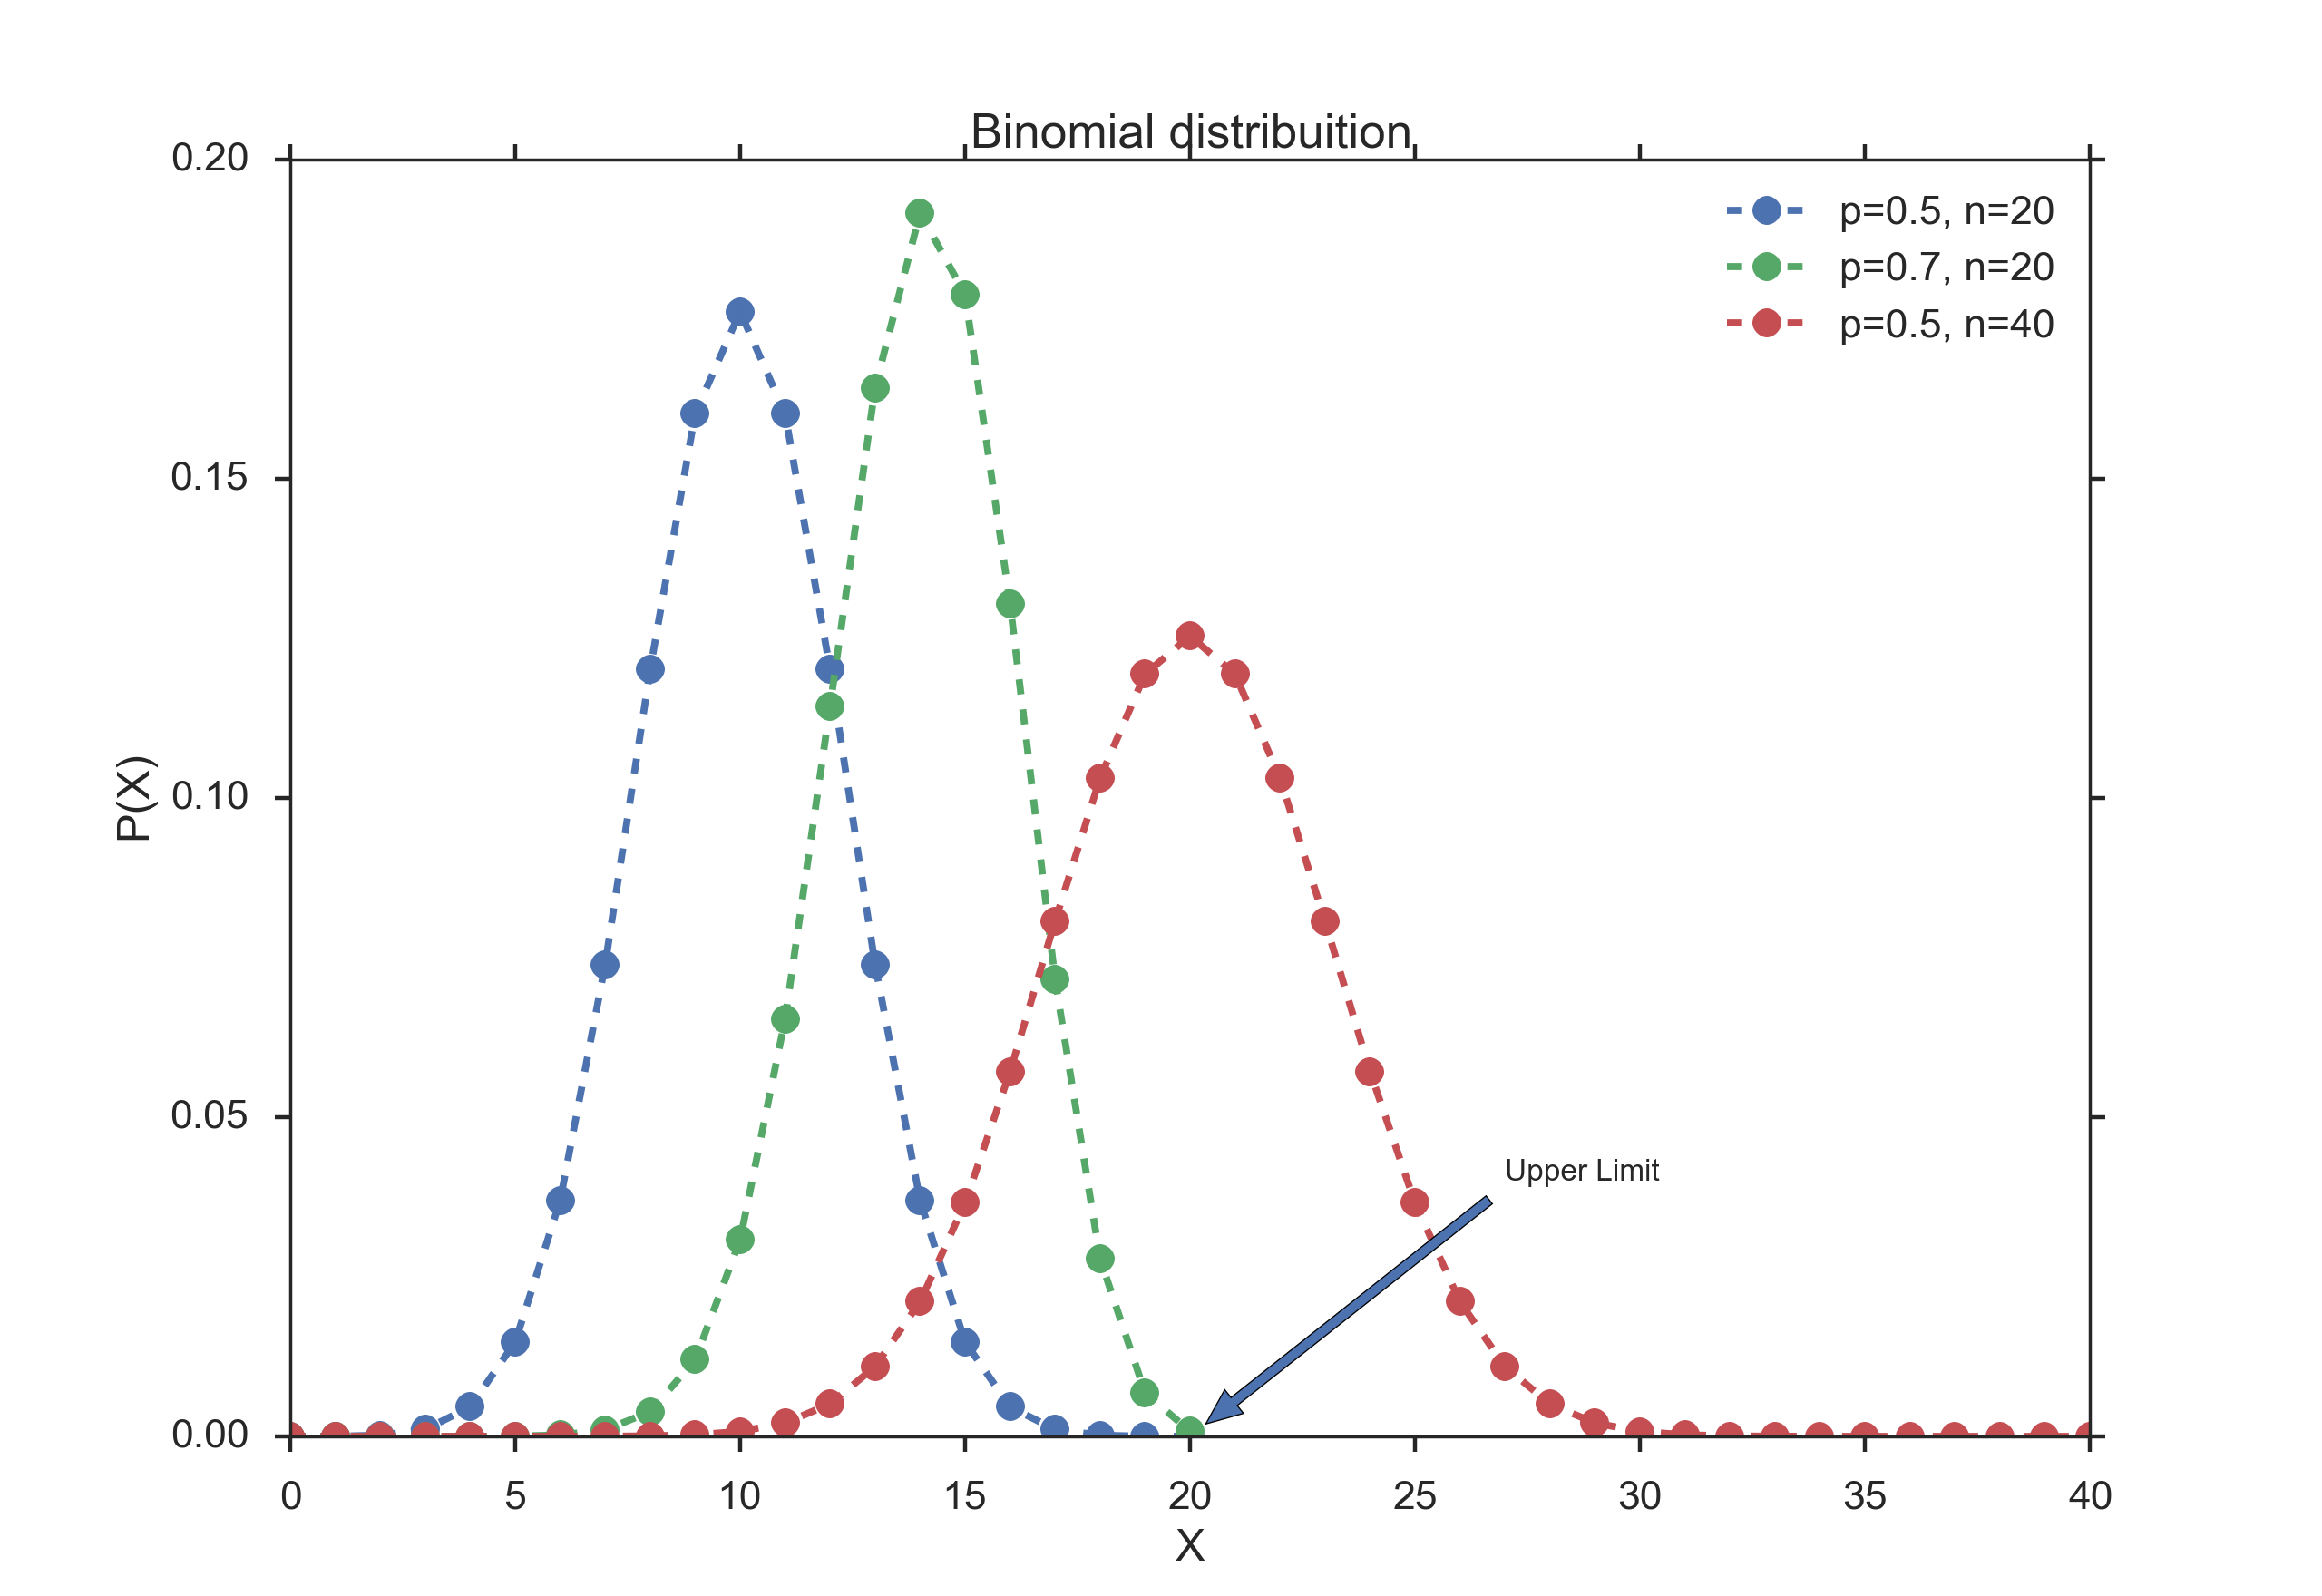
\includegraphics[width=0.66\textwidth]{../Images/Binomial_distribution_pmf.png}\\
  \caption{Binomial Distribution. Note that legal values exist only for integer x. The dotted lines in between only facilitate the grouping of the values to individual distribution parameters.}
\end{figure}


\paragraph{Example: Binomial Test}\index{general}{test!binomial}

Suppose we have a board game that depends on the roll of a die and attaches special importance to rolling a 6. In a particular game, the die is rolled 235 times, and 6 comes up 51 times. If the die is fair, we would expect 6 to come up 235/6 = 39.17 times. Is the proportion of 6's significantly higher than would be expected by chance, on the null hypothesis of a fair die?

To find an answer to this question using the Binomial Test, we consult the binomial distribution with n=235 and p=1/6, to determine the probability of finding exactly 51 sixes in a sample of 235 if the true probability of rolling a 6 on each trial is 1/6. We then find the probability of finding exactly 52, exactly 53, and so on up to 235, and add all these probabilities together. In this way, we calculate the probability of obtaining the observed result (51 6s) or a more extreme result ($>51 6's$) assuming that the die is fair. In this example, the result is 0.0265, which indicates that observing 51 6's is unlikely (significant at the 5\% level) to come from a die that is not loaded to give many 6's (one-tailed test).

Clearly a die could roll too few sixes as easily as too many and we would be just as suspicious, so we should use the two-tailed test which (for example) splits the 5\% probability across the two tails.

\PyImg "binomial.py" (p \pageref{py:binomial}): Example of a one-and two-sided binomial test.
\index{python}{binomialTest}

\begin{table}[h]
  \centering
  \begin{tabular}{l|c|c|}
      & Mean & Variance \\
      \hline
      Binomial & $n \cdot p$ & $np(1-p)$ \\
      Poisson & $\lambda$ & $\lambda$ \\
      %\hline
  \end{tabular}
\caption{Properties of discrete distributions.}
\end{table}

\subsection{Poisson Distribution}\index{general}{distributions!poisson}

Any French speaker will notice that "Poisson" means "fish", but really there's nothing fishy about this distribution. It's actually pretty straightforward. The name comes from the mathematician Siméon-Denis Poisson (1781-1840).

The Poisson Distribution is ''very similar'' to the Binomial Distribution. We are examining the number of times an event happens. The difference is subtle. Whereas the Binomial Distribution looks at how many times we register a success over a fixed total number of trials, the Poisson Distribution measures how many times a discrete event occurs, over a period of continuous space or time. There is no "total" value n. As with the previous sections, let's examine a couple of experiments or questions that might have an underlying Poisson nature.

\begin{itemize}
  \item How many pennies will I encounter on my walk home?
  \item How many children will be delivered at the hospital today?
  \item How many products will I sell after airing a new television commercial?
  \item How many mosquito bites did you get today after having sprayed with insecticide?
  \item How many defects will there be per 100 metres of rope sold?
\end{itemize}

What's a little different about this distribution is that the random variable $X$ which counts the number of events can take on any non-negative integer value. In other words, I could walk home and find no pennies on the street. I could also find one penny. It's also possible (although unlikely, short of an armored-car exploding nearby) that I would find 10 or 100 or 10,000 pennies.

Instead of having a parameter p that represents a component probability like in the Binomial distribution, this time we have the parameter "lambda" or $\lambda$ which represents the "average or expected" number of events to happen within our experiment. The probability mass function of the Poisson is given by

\begin{equation}
  P(X=k)=\frac{e^{-\lambda}\lambda^k}{k!}
\end{equation}.

\begin{figure}
  \centering
  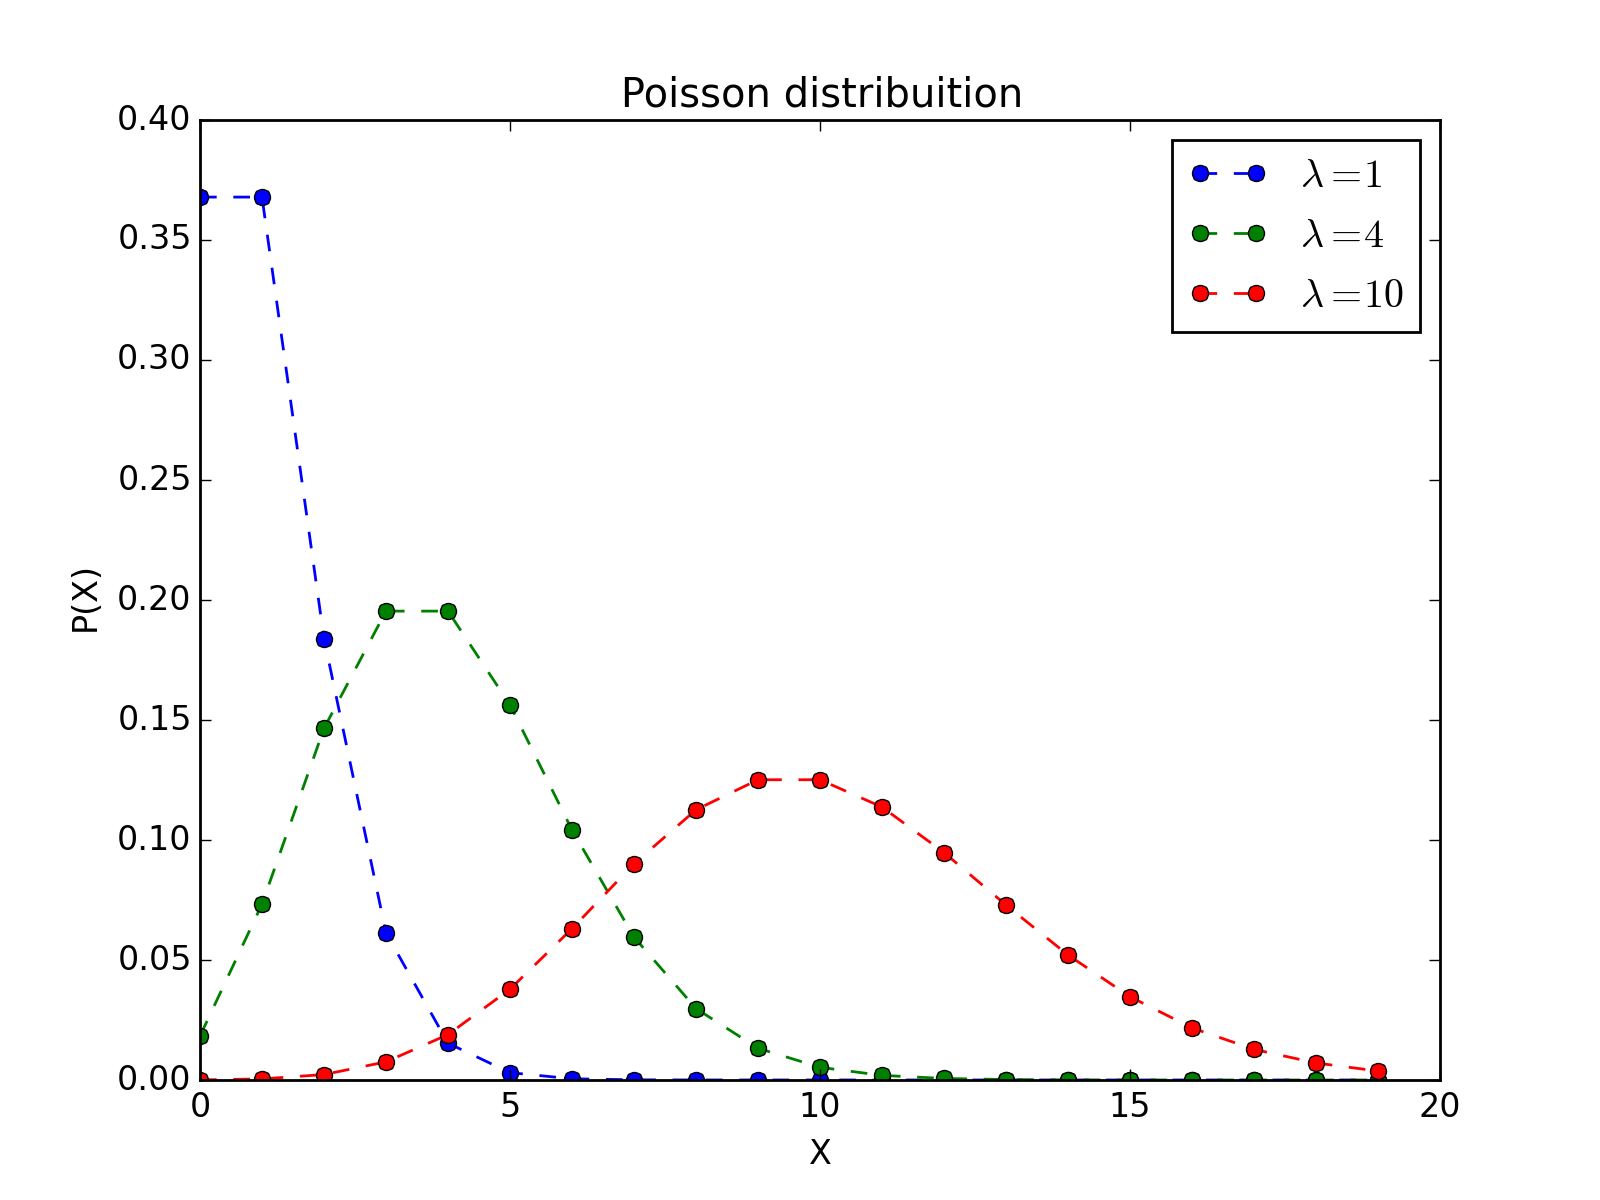
\includegraphics[width=0.66\textwidth]{../Images/Poisson_distribution_pmf.png}\\
  \caption{Poisson Distribution. Again note that legal values exist only for integer x. The dotted lines in between only facilitate the grouping of the values to individual distribution parameters.}
\end{figure}

\subsection{Programs: Discrete Distribution Functions} \index{general}{distributions!discrete}

\vspace{5 mm}

\PyImg "distributionDiscrete.py" (p \pageref{py:discrete}) shows different continuous distribution functions.
\index{python}{distributionDiscrete}
%(Lecture 7)


\section{Continuous Distribution}

Many measurements have an outcome that is not restricted to discrete integer values. For example, the weight of a person can be any positive number. In that case, the probability that a certain value comes up is described by a continuous function, the "Probability Density Function (PDF)"\index{general}{probability density function}.

The \acrfull{pdf}, or \gls{density} of a continuous random variable, is a function that describes the relative likelihood for a random variable $X$ to take on a given value $x$.
In the mathematical fields of probability and statistics, a "random variate" x \index{general}{random variate} is a particular outcome of a "random variable" X: the random variates which are other outcomes of the same random variable might have different values.

Since the likelihood to find any given value cannot be less than zero, and since the variable has to have some value, the PDF has the following properties:

\begin{itemize}
  \item $PDF(x) \geq 0\,\forall \,x \in \mathbb{R}$
  \item $ \int\limits_{ - \infty }^\infty  {PDF(x)dx = 1} $
\end{itemize}

The PDF also defines the expected value E[x] \index{general}{expected value} of a continuous distribution of X:

\begin{equation}\label{eq:expectedValue}
   \operatorname{E}[X] = \int_{-\infty}^\infty x f(x)\, \mathrm{d}x .
\end{equation}

\begin{figure}
  \centering
  % Requires \usepackage{graphicx}
  \includegraphics[width=0.5\textwidth]{../Images/PDF.png}\\
  \caption{Probability Density Function (PDF) of a value x. The integral over the PDF between a and b gives the likelihood of finding the value of x in that range.}
  \label{fig:PDF}
\end{figure}

\section{Characterizing a Distribution}

In addition to the "probability mass function (PMF)" for discrete distributions, and the corresponding "probability density function (PDF)" for continuous distributions, probability distributions has many other methods associated with it:

\subsubsection{Cumulative Distribution Function (CDF)}\index{general}{cumulative distribution function}

The probability to find a value between $a$ and $b$ is given by the integral over the PDF in that range (see Fig. \ref{fig:PDF}). The \gls{cdf_} \acrshort{cdf}, which is the integral from minus infinity up to the given value, and which specifies which percentage of the data below that value (Figure \ref{fig:CDF}), facilitates that calculation:

\begin{equation}
   \mathbb{P}(a \leq X \leq b) = \int\limits_a^b {PDF(x)dx} = CDF(b) - CDF(a)
\end{equation}

For discrete distributions, the integral has to be replaced by a sum.

\begin{figure}[ht]
  \centering
  \includegraphics[width=0.5\textwidth]{../Images/PDF_CDF.png}\\
  \caption{\emph{Probability density function} (left) and \emph{Cumulative distribution function} (right) of a normal distribution.}\label{fig:CDF}
\end{figure}

\subsubsection{Other important presentations of Probability Densities}\index{general}{cumulative distribution function}

Figure \ref{fig:DistributionUtilities} shows a number of functions that are equivalent to the PDF, but each represent a different aspect of the probability distribution. I will give examples which demonstrate each aspect for a normal distribution describing the size of male subjects.

\begin{itemize}
  \item \emph{Probability density function (PDF)}: note that to obtain the probability for the variable appearing in a certain interval, you have to \emph{integrate} the PDF over that range.

      Example: What is the chance that a man is between 160 and 165 cm tall?

  \item \emph{Cumulative distribution function (CDF)}: gives the probability of obtaining a value smaller than the given value.

        Example: What is the chance that a man is less than 165 cm tall?

  \item \emph{\acrfull{sf} (SF)}: 1-CDF: gives the probability of obtaining a value larger than the given value. It can also be interpreted as the proportion of data "surviving" above a certain value.

      Example: What is the chance that a man is larger than 165 cm?

  \item \emph{\acrfull{ppf} (PPF)}: the inverse of the CDF. Answers the question "Given a certain probability, what is the corresponding value for the CDF?"

    Example: Given that I am looking for a man who is smaller than 95\% of all other men, what size does the subject have to be?

  \item \emph{\acrfull{isf} (ISF)}: the name says it all.

      Example: Given that I am looking for a man who is larger than 95\% of all other men, what size does the subject have to be?

  \item \acrfull{rvs} \emph{(RVS)}: random variates\index{general}{variate} from a given distribution. (A \emph{variable} is the general type, a \emph{variate} is a specific number.)

\end{itemize}

\begin{figure}
  \centering
  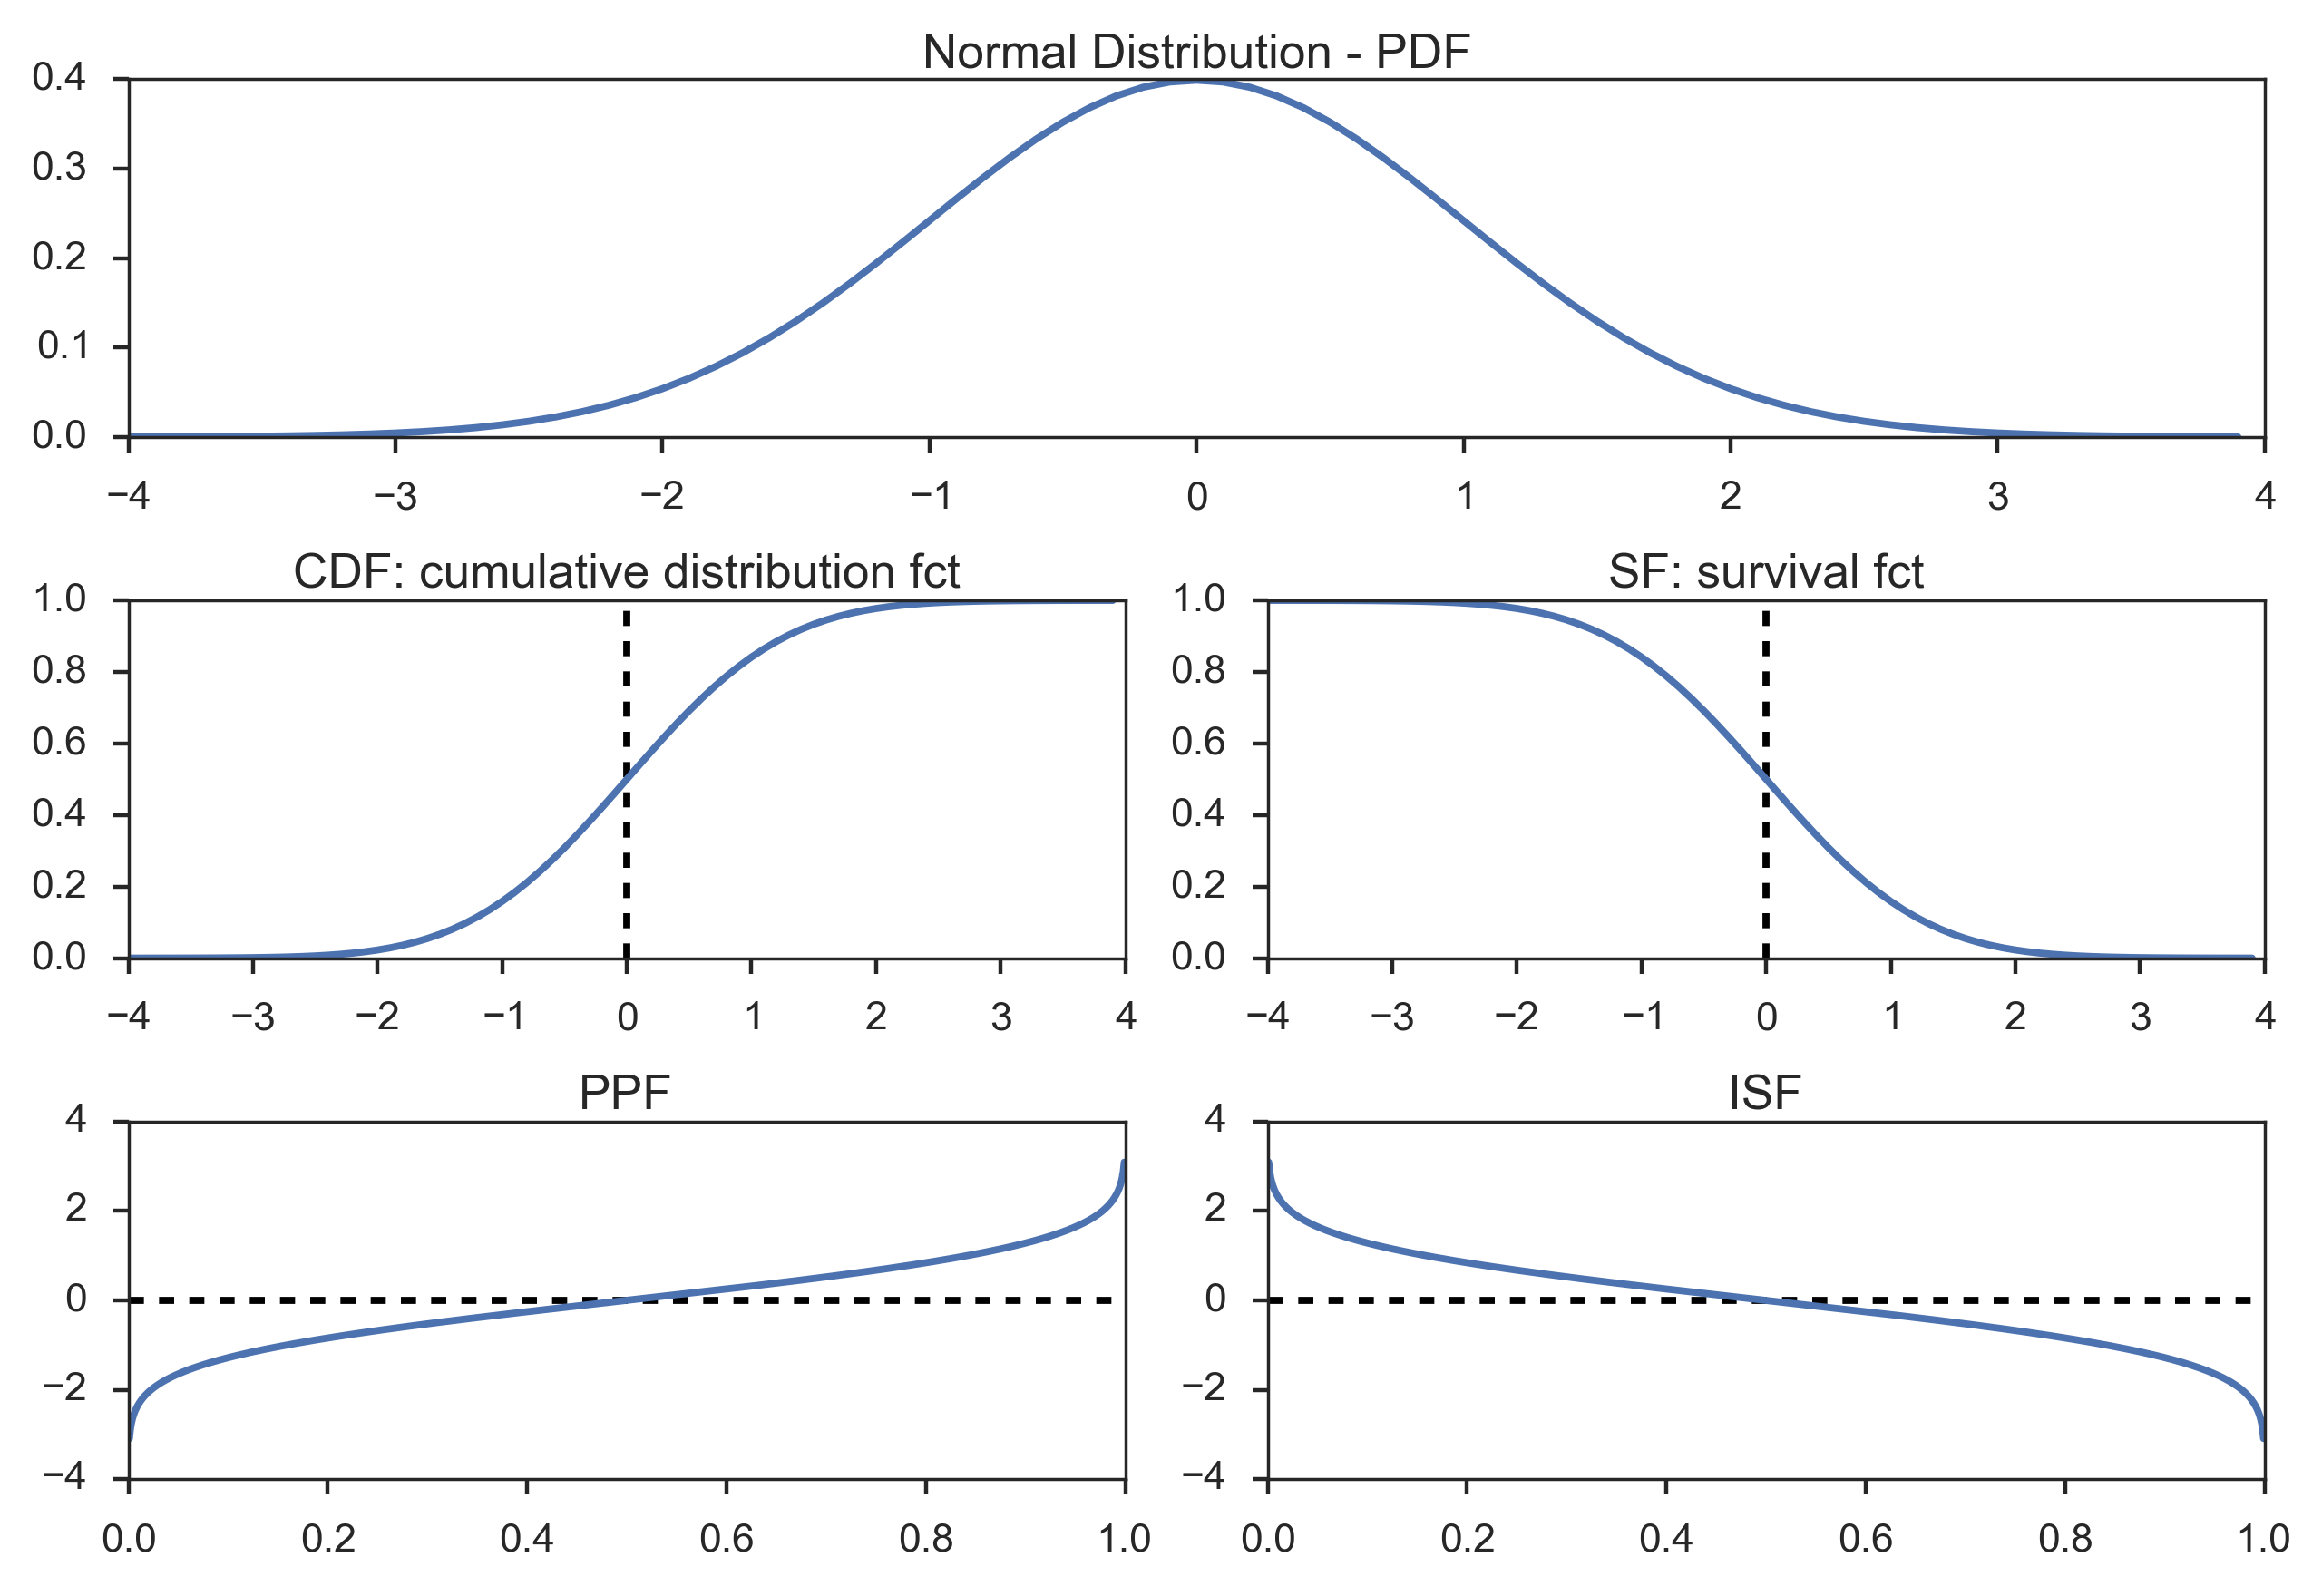
\includegraphics[width=0.95\textwidth]{../Images/DistributionFunctions.png}\\
  \caption{Utility functions for continuous distributions, here for the normal distribution.}\label{fig:DistributionUtilities}
\end{figure}

\vspace{5 mm}
\fbox{%
\begin{minipage}{15 cm}

\textbf{Note:}
In \emph{Python}, the most elegant way of working with distribution function is a two-step procedure:
\begin{itemize}
  \item In the first step, you create your distribution (e.g. \textsf{nd = stats.norm()}). Note that is a distribution (in \emph{Python} parlance a "frozen distribution"\index{general}{frozen distribution}), not a function yet!
  \item In the second step, you decide which function you want to use from this distribution, and calculate the function value for the desired x-input (e.g. \textsf{y = nd.cdf(x)})
\end{itemize}

\end{minipage}}

\begin{lstlisting}[language=Python]
  In [1]: import numpy as np
  In [2]: from scipy import stats
  In [3]: myDF = stats.norm(5,3)
  In [4]: x = np.linspace(-5, 15, 101)
  In [5]: y = myDF.pdf(x)
\end{lstlisting}


\vspace{10 mm}

\subsection{Distribution Center}\index{general}{distribution center}

When we have a datasample from a distribution, we can characterize the center of the distribution with different parameters. Thereby the data can be evaluated in two ways:

\begin{enumerate}
  \item By their value.
  \item By their \gls{rank} (i.e. their list-number when they are ordered according to magnitude).
\end{enumerate}

\subsubsection{Mean} \index{general}{mean}
By default, when we talk about the mean value we mean the arithmetic mean $\bar{x}$:

\begin{equation}
  \bar{x} = \frac{{\sum\limits_{i = 1}^n {{x_i}} }}{n}
\end{equation}

\subsubsection{Median} \index{general}{median}
The \gls{median} is that value that comes half-way when the data are ranked in order.
In contrast to the mean, the median is not affected by outlying data points.

\subsubsection{Mode} \index{general}{mode}
The \gls{mode} is the most frequently occurring value in a distribution.

\subsubsection{Geometric Mean}\index{general}{geometric mean}
In some situations the geometric mean can be useful to describe the location of a distribution. It is usually close to the median, and can be calculated via the arithmetic mean of the log of the values.

\begin{equation}\label{eq:geometricMean}
  mean_{geometric} =  \left(\prod_{i=1}^N x_i\right)^{1/N} = e^{\left( \frac{\sum_i ln(x_i)}{n} \right)}
\end{equation}

\subsection{Quantifying Variability}\label{sec:centiles}

\subsubsection{Range}\index{general}{range}

This one is fairly easy: it is the difference between the highest and the lowest data value.
The only thing that should be watched are outliers, i.e. data points with a value much higher or lower than the rest of the data. Often, such points are caused by errors in the selection of the sample or in the measurement procedure. There are a number of tests to check for outliers. One of them is to check for data which lie more than 1.5*inter-quartile-range (IQR) above or below the first/third quartile (see below).


\subsubsection{Percentiles}\index{general}{centiles}\index{general}{percentiles}

Centiles, also called "\glspl{percentile}", give the value below which a given percentage of the data values occur. Centiles correspond to the cumulative frequency. While the expression "centiles" does not come up very often, one will frequently encounter specific centiles:

\begin{itemize}
  \item To find the range which includes 95\% of the data, one have to find the $2.5^{th}$ and the $97.5^{th}$ percentile of the sample distribution.
  \item The 50th percentile is the "median".
  \item Also important are the "quartiles", i.e. the $25^{th}$ and the $75^{th}$ percentile. The difference between them is called the "inter-quartile range" (IQR)\index{general}{inter-quartile-range, IQR}.
\end{itemize}

Median, upper and lower quartile are used for the data display in box plots (Fig. \ref{fig:Boxplot}).

\subsubsection{Standard Deviation and Variance}

In Fig. \ref{fig:population} I have sketched out how to use the sample statistic to learn about the corresponding population parameter. In the following we distinguish between the "sample variance", i.e. the variance in the data sampled, and the "population variance", i.e. the variance of the full population. The maximum likelihood estimator of the sample \gls{variance} is given by

\begin{equation}\label{eq:variance} \index{general}{variance}
  var = \frac{{\sum\limits_{i = 1}^n {({x_i-\bar{x}})^2} }}{n}
\end{equation}

However, Eq. \ref{eq:variance} systematically underestimates the population variance, and is therefore referred to as a "biased estimator"\index{general}{biased estimator} of the population variance. Figure \ref{fig:mean_std} tries to motivate why the sample variance underestimates the population variance: the sample mean is always chosen such that the variance of the sample data gets minimized.

\begin{figure}[ht]
  \centering
  \includegraphics[width=0.5\textwidth]{../Images/mean_std.png}\\
  \caption{Gaussian distributions fitted to selections of data from the underlying distribution: While the average mean of a number of samples converges to the real mean, the sample standard deviation underestimates the standard deviation from the distribution.}\label{fig:mean_std}
\end{figure}

The best unbiased estimator for the population variance is given by

\begin{equation}\label{eq:sampleVariance}
  var = \frac{{\sum\limits_{i = 1}^n {({x_i-\bar{x}})^2} }}{n-1}
\end{equation}

Eq. \ref{eq:sampleVariance} is referred to as "sample variance"\index{general}{sample variance}.

The \gls{sd_} \index{general}{standard deviation}\index{general} is the square root of the variance, and the
"sample standard deviation"\index{general}{sample satandard deviation} the square root of the "sample variance":

\begin{equation}
  s = \sqrt{var}
\end{equation}

As mentioned in Table \ref{table:population}, in statistics it is common to denote the population standard deviation with $\sigma$, and the sample standard deviation with $s$.

Watch out: in \emph{Python}, by default the variance is calculated for "n". You have to set "ddof=1" to obtain the variance for "n-1":

\begin{lstlisting}[language=Python]
    In[19]: data = arange(7,14)

    In[20]: std(data, ddof=0)
    Out[20]: 2.0

    In[21]: std(data, ddof=1)
    Out[21]: 2.1602468994692865
\end{lstlisting}

\subsubsection{Standard Error} \index{general}{standard error}

The "standard error" is the estimate of the standard deviation of a coefficient. For example, in Fig. \ref{fig:sem}, we have 100 datapoints from a normal distribution about $5$. The more datapoints we have to estimate the mean value, the better our estimate of the mean.

\begin{figure}[ht]
  \centering
  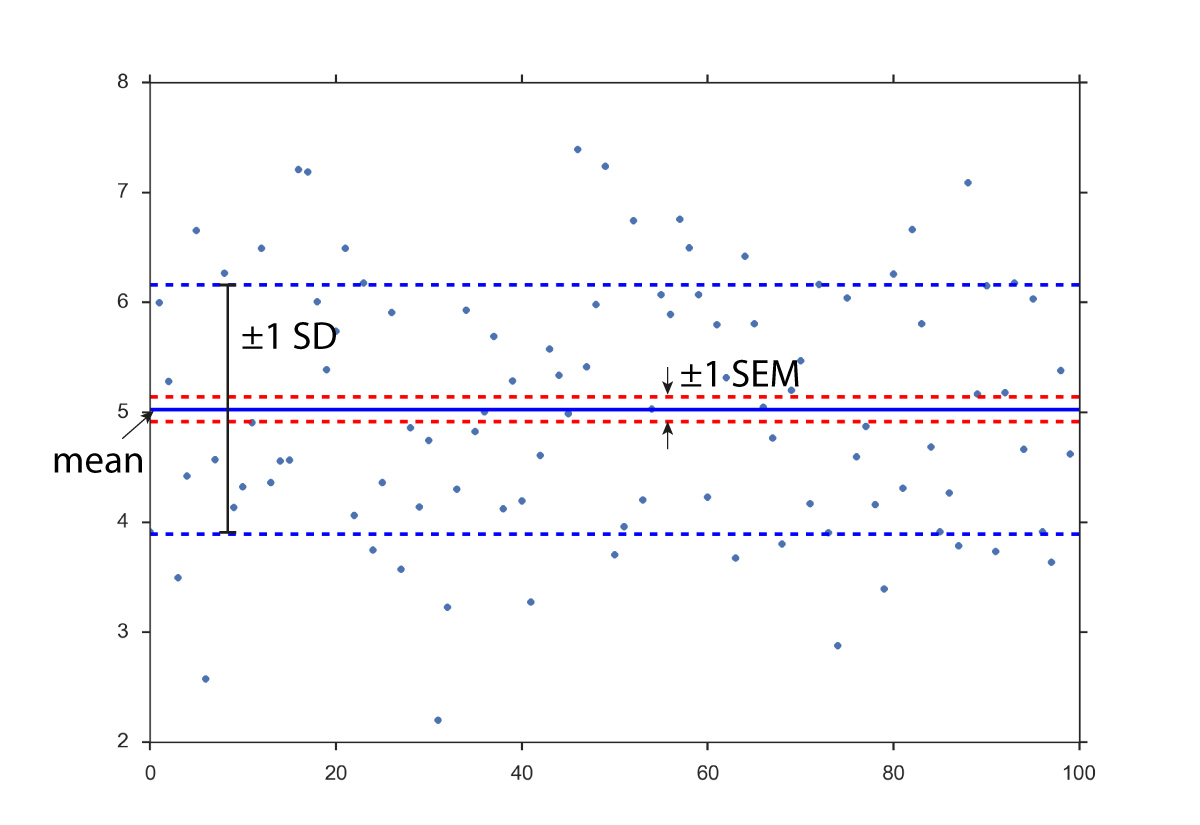
\includegraphics[width=0.66\textwidth]{../Images/standardError.jpg}\\
  \caption{100 random data points, from a normal distribution about 5. The sample mean is very close to the real mean. The standard deviation of the mean, or standard error is 10 times smaller than the standard deviation of the samples.}
  \label{fig:sem}
\end{figure}

For normally distributed data, the sample standard error of the mean (SE or SEM) is

\begin{equation}
  SE = \frac{s}{\sqrt{n}} = \sqrt{\frac{{\sum\limits_{i = 1}^n {({x_i-\bar{x}})^2} }}{n-1}} \cdot \frac{1}{\sqrt{n}}
\end{equation}

So with 100 datapoints the standard deviation of our estimate, i.e. the standard error of the mean, is 10 times smaller than the sample standard deviation.

\subsubsection{Confidence Intervals}\index{general}{confidence interval}

 In the statistical analysis of data it has become common to state the \acrfull{ci} of an estimated parameter. The \gls{confidenceinterval} reports the range that contains the true value for your parameter with a likelihood of $\alpha$\%.

If the sampling distribution is symmetrical and unimodal, it will often be possible to approximate the confidence interval by

\begin{equation}\
  ci = mean \pm std * N_{ISF}(\alpha)
\end{equation}\label{eq:ci}

where $std$ is the  standard deviation, and $N_{ISF}(\alpha)$ the inverse survival function for the normal distribution. For the 95\% two-sided confidence intervals, for example, you have to set $\alpha=0.025$ and $\alpha=0.975$ .

\textbf{Note:} For the confidence interval for the mean value, the standard deviation has to be replaced by the standard error!

\subsection{Parameters Describing the Form of a Distribution}

In \texttt{scipy.stats}, continuous distribution functions are characterized by their "location" and their "scale".
For example, for the normal distribution, (location/shape) are given by (mean/standard deviation) of the distribution. In contrast, for the uniform distribution, (location/shape) are given by the (start/end) of the range where the distribution is different from zero.

\subsubsection{Location}\index{general}{distribution!location}

A \gls{location} parameter $x_0$  determines the "location" or shift of a distribution:

\begin{equation*}
  f_{x0}(x)=f(x-x_0)
\end{equation*}

Examples of location parameters include the mean, the median, and the mode.

\subsubsection{Scale}\index{general}{distribution!scale}

The \gls{scale} parameter describes the width of a probability distribution.  If s is large, then the distribution will be more spread out; if s is small then it will be more concentrated. If the probability density exists for all values of $s$, then the density (as a function of the scale parameter only) satisfies

\begin{equation*}
   f_s(x) = f(x/s)/s,
\end{equation*}

where f is the density of a standardized version of the density.

\subsubsection{Shape Parameters}\index{general}{shape parameters}

It is customary to refer to all of the parameters beyond location and scale as \glspl{shapeparameter}. Thankfully, almost all of the distributions that we use in statistics have only one or two parameters. It follows that the \gls{skewness} and \gls{kurtosis} of these distribution are constants.

\begin{figure}
  \centering
  \includegraphics[width=0.66\textwidth]{../Images/Skewness.png}\\
  \caption{Left) Normal distribution, and distribution with positive skewness. Right) The (leptokurtic) Laplace distribution has an excess kurtosis of 3, and the (platykurtic) Wigner semicircle distribution an excess kurtosis of -1.}\label{fig:skewkurtosis}
\end{figure}

\subsubsection{Skewness}\index{general}{skewness}

Distributions are "skewed" if they depart from symmetry (Fig. \ref{fig:skewkurtosis}, left). For example, for measurements that cannot be negative, which is usually the case, we can infer that the data have a skewed distribution if the standard deviation is more than half the mean. Such an asymmetry is referred to as "positive skewness". The opposite, negative skewness, is rare.

\subsubsection{Kurtosis}\index{general}{kurtosis}

Kurtosis is a measure of the "peakedness" of the probability distribution (Fig. \ref{fig:skewkurtosis}, right), where the normal distribution is taken as the standard refernence. Distributions with negative or positive excess kurtosis are called Platykurtic Distributions or Leptokurtic Distributions, respectively.

\section{Normal Distribution} \label{sec:normalDistribution}\index{general}{distributions!normal}\index{general}{normal distribution}\index{general}{Gaussian distribution}

The Normal distribution or Gaussian distribution is by far the most important of all the distribution functions. This is due to the fact that the mean values of \emph{all} distribution functions approximate a normal distribution for large enough sample numbers (see chapter \ref{sec:CentralLimitTheorem}).
Mathematically, the normal distribution is characterized by a mean value $\mu$, and a standard deviation $\sigma$:

\begin{equation}\label{eq_normal}
     f_{\mu,\sigma} (x) = \frac{1}{\sigma \sqrt{2 \pi}} e^{-( x - \mu )^2 /2 \sigma^2}
\end{equation}
where $ - \infty < x < \infty $, and $f_{\mu,\sigma}$ is the \gls{pdf_} (PDF) \index{general}{probability density function} of the normal distribution.

\begin{figure}
  \centering
  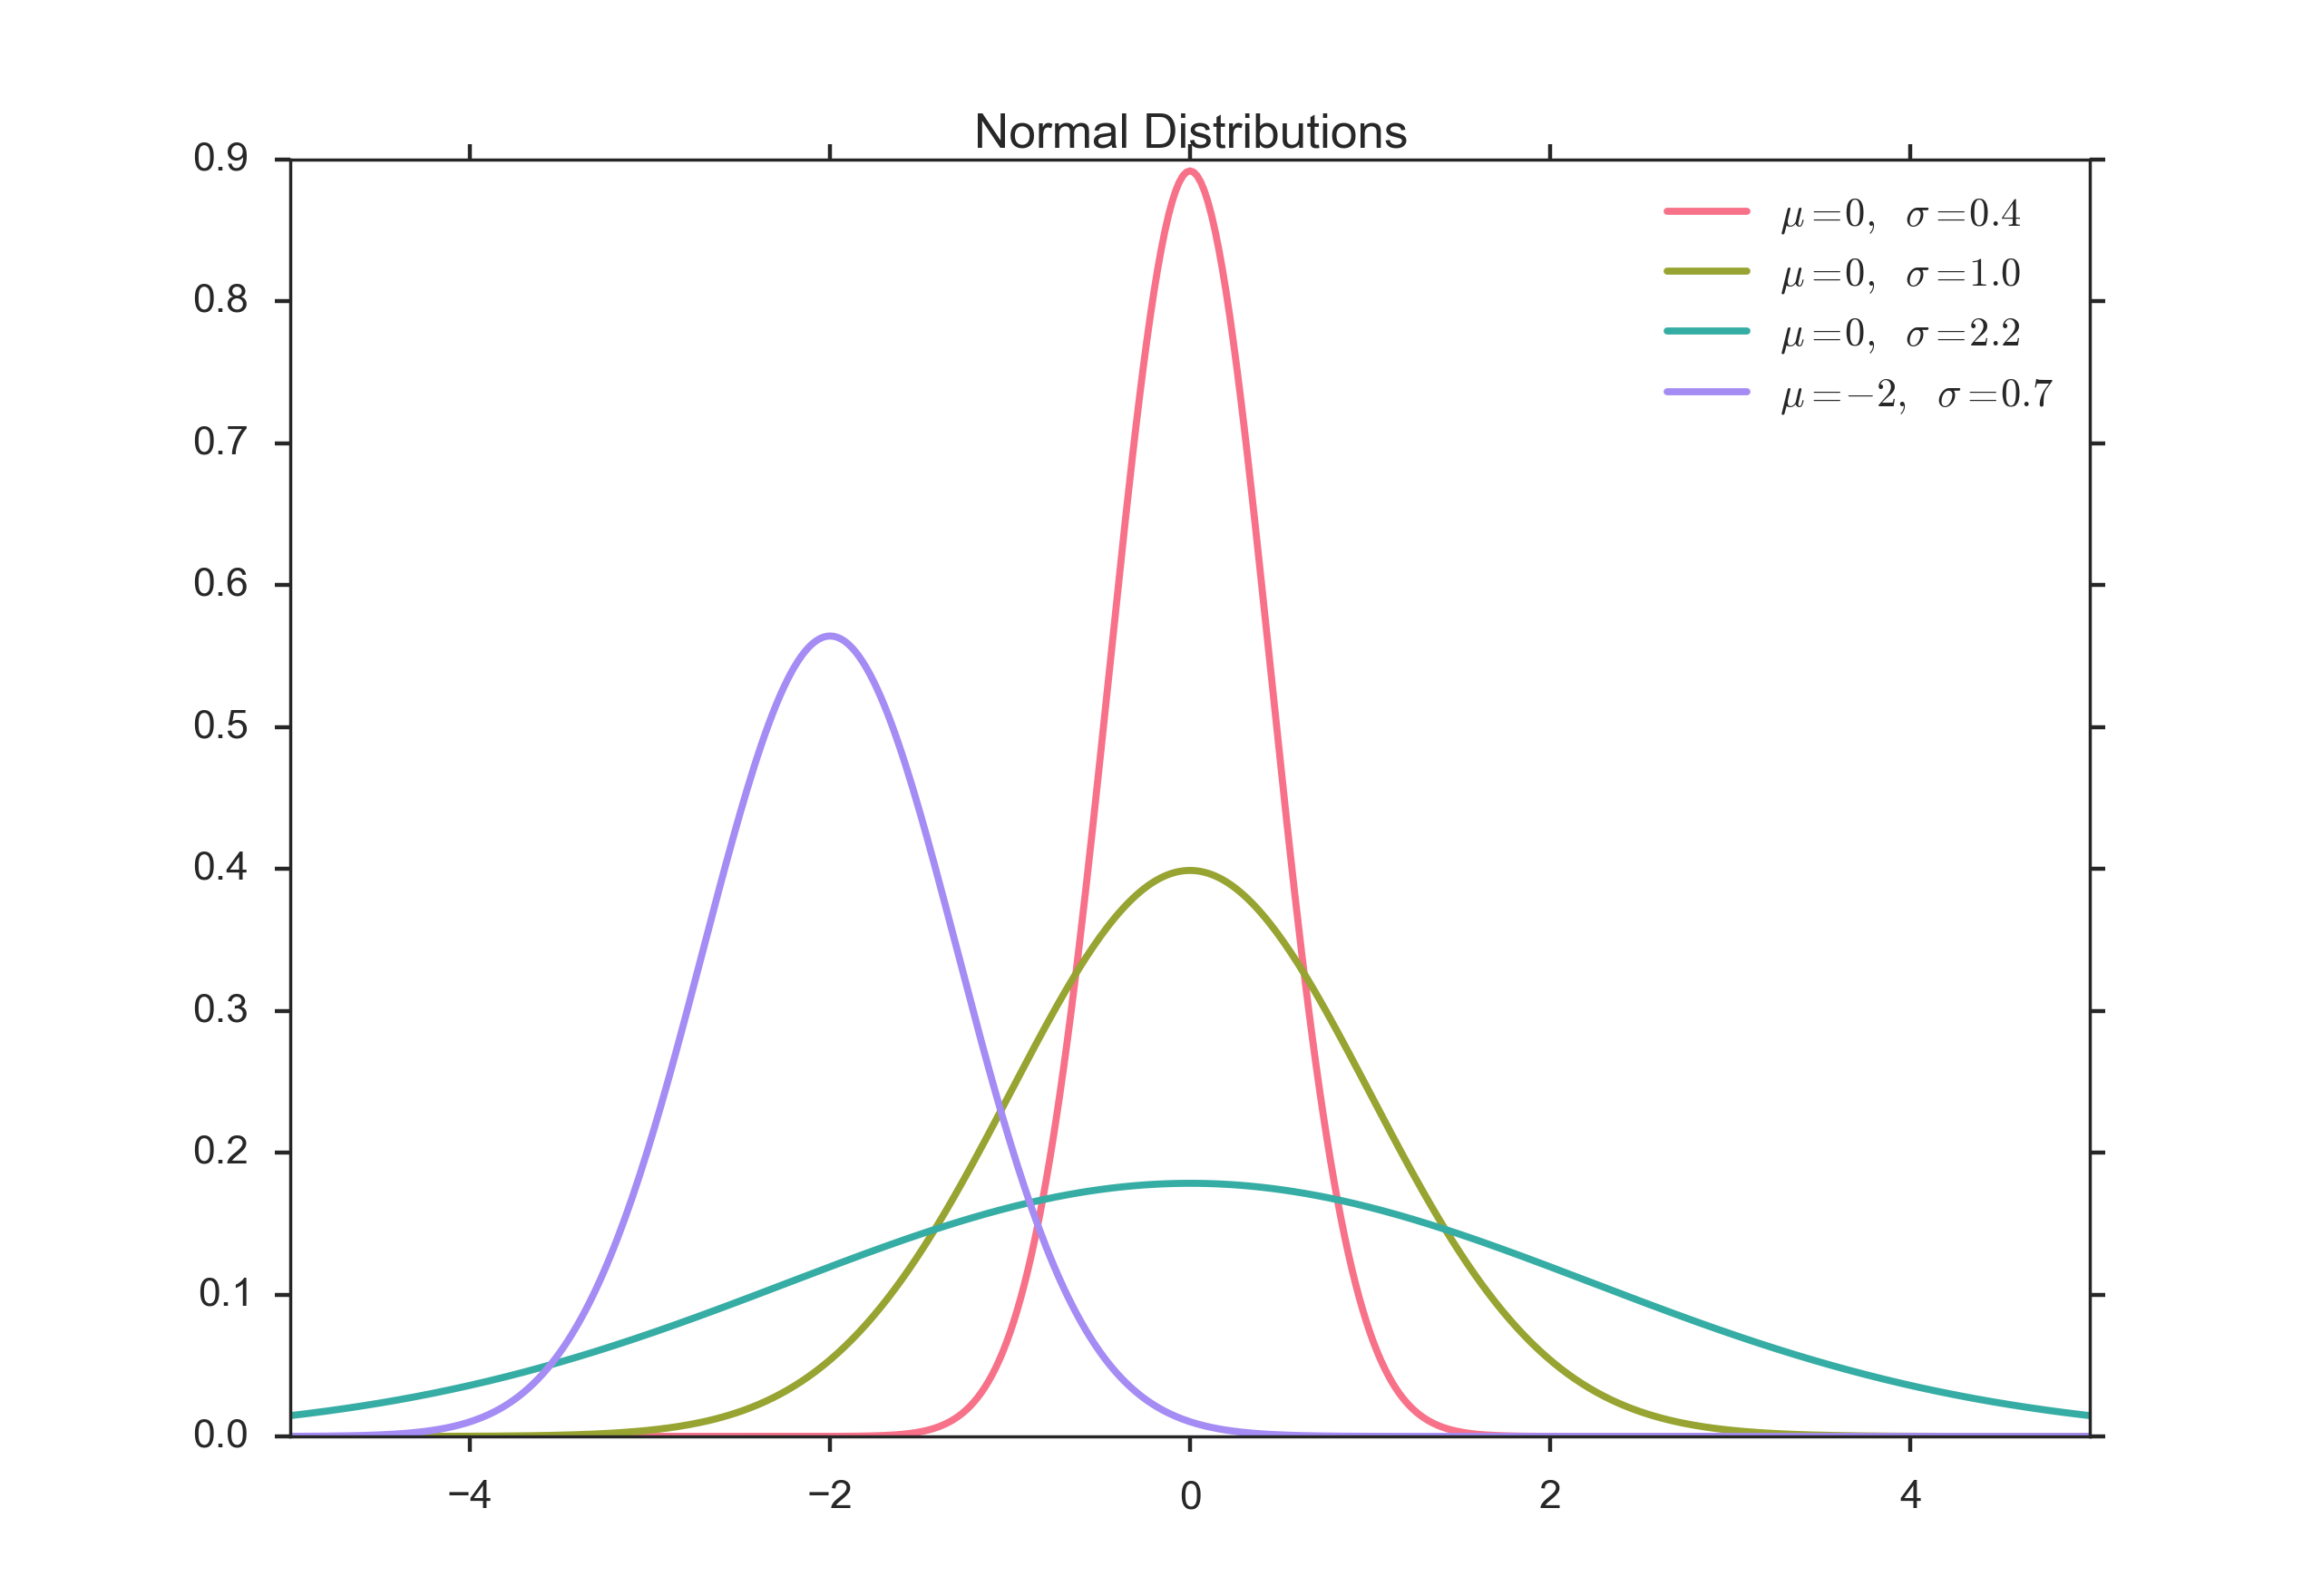
\includegraphics[width=0.75\textwidth]{../Images/Normal_Distribution_PDF.png}\\
  \caption{Normal Distribution}\label{fig:normal}
\end{figure}

For smaller sample numbers, the sample distribution can show quite a bit of variability. For example, look at 25 distributions generated by sampling 100 numbers from a normal distribution (Fig. \ref{fig:MultipleNormal})

\begin{figure}
  \centering
  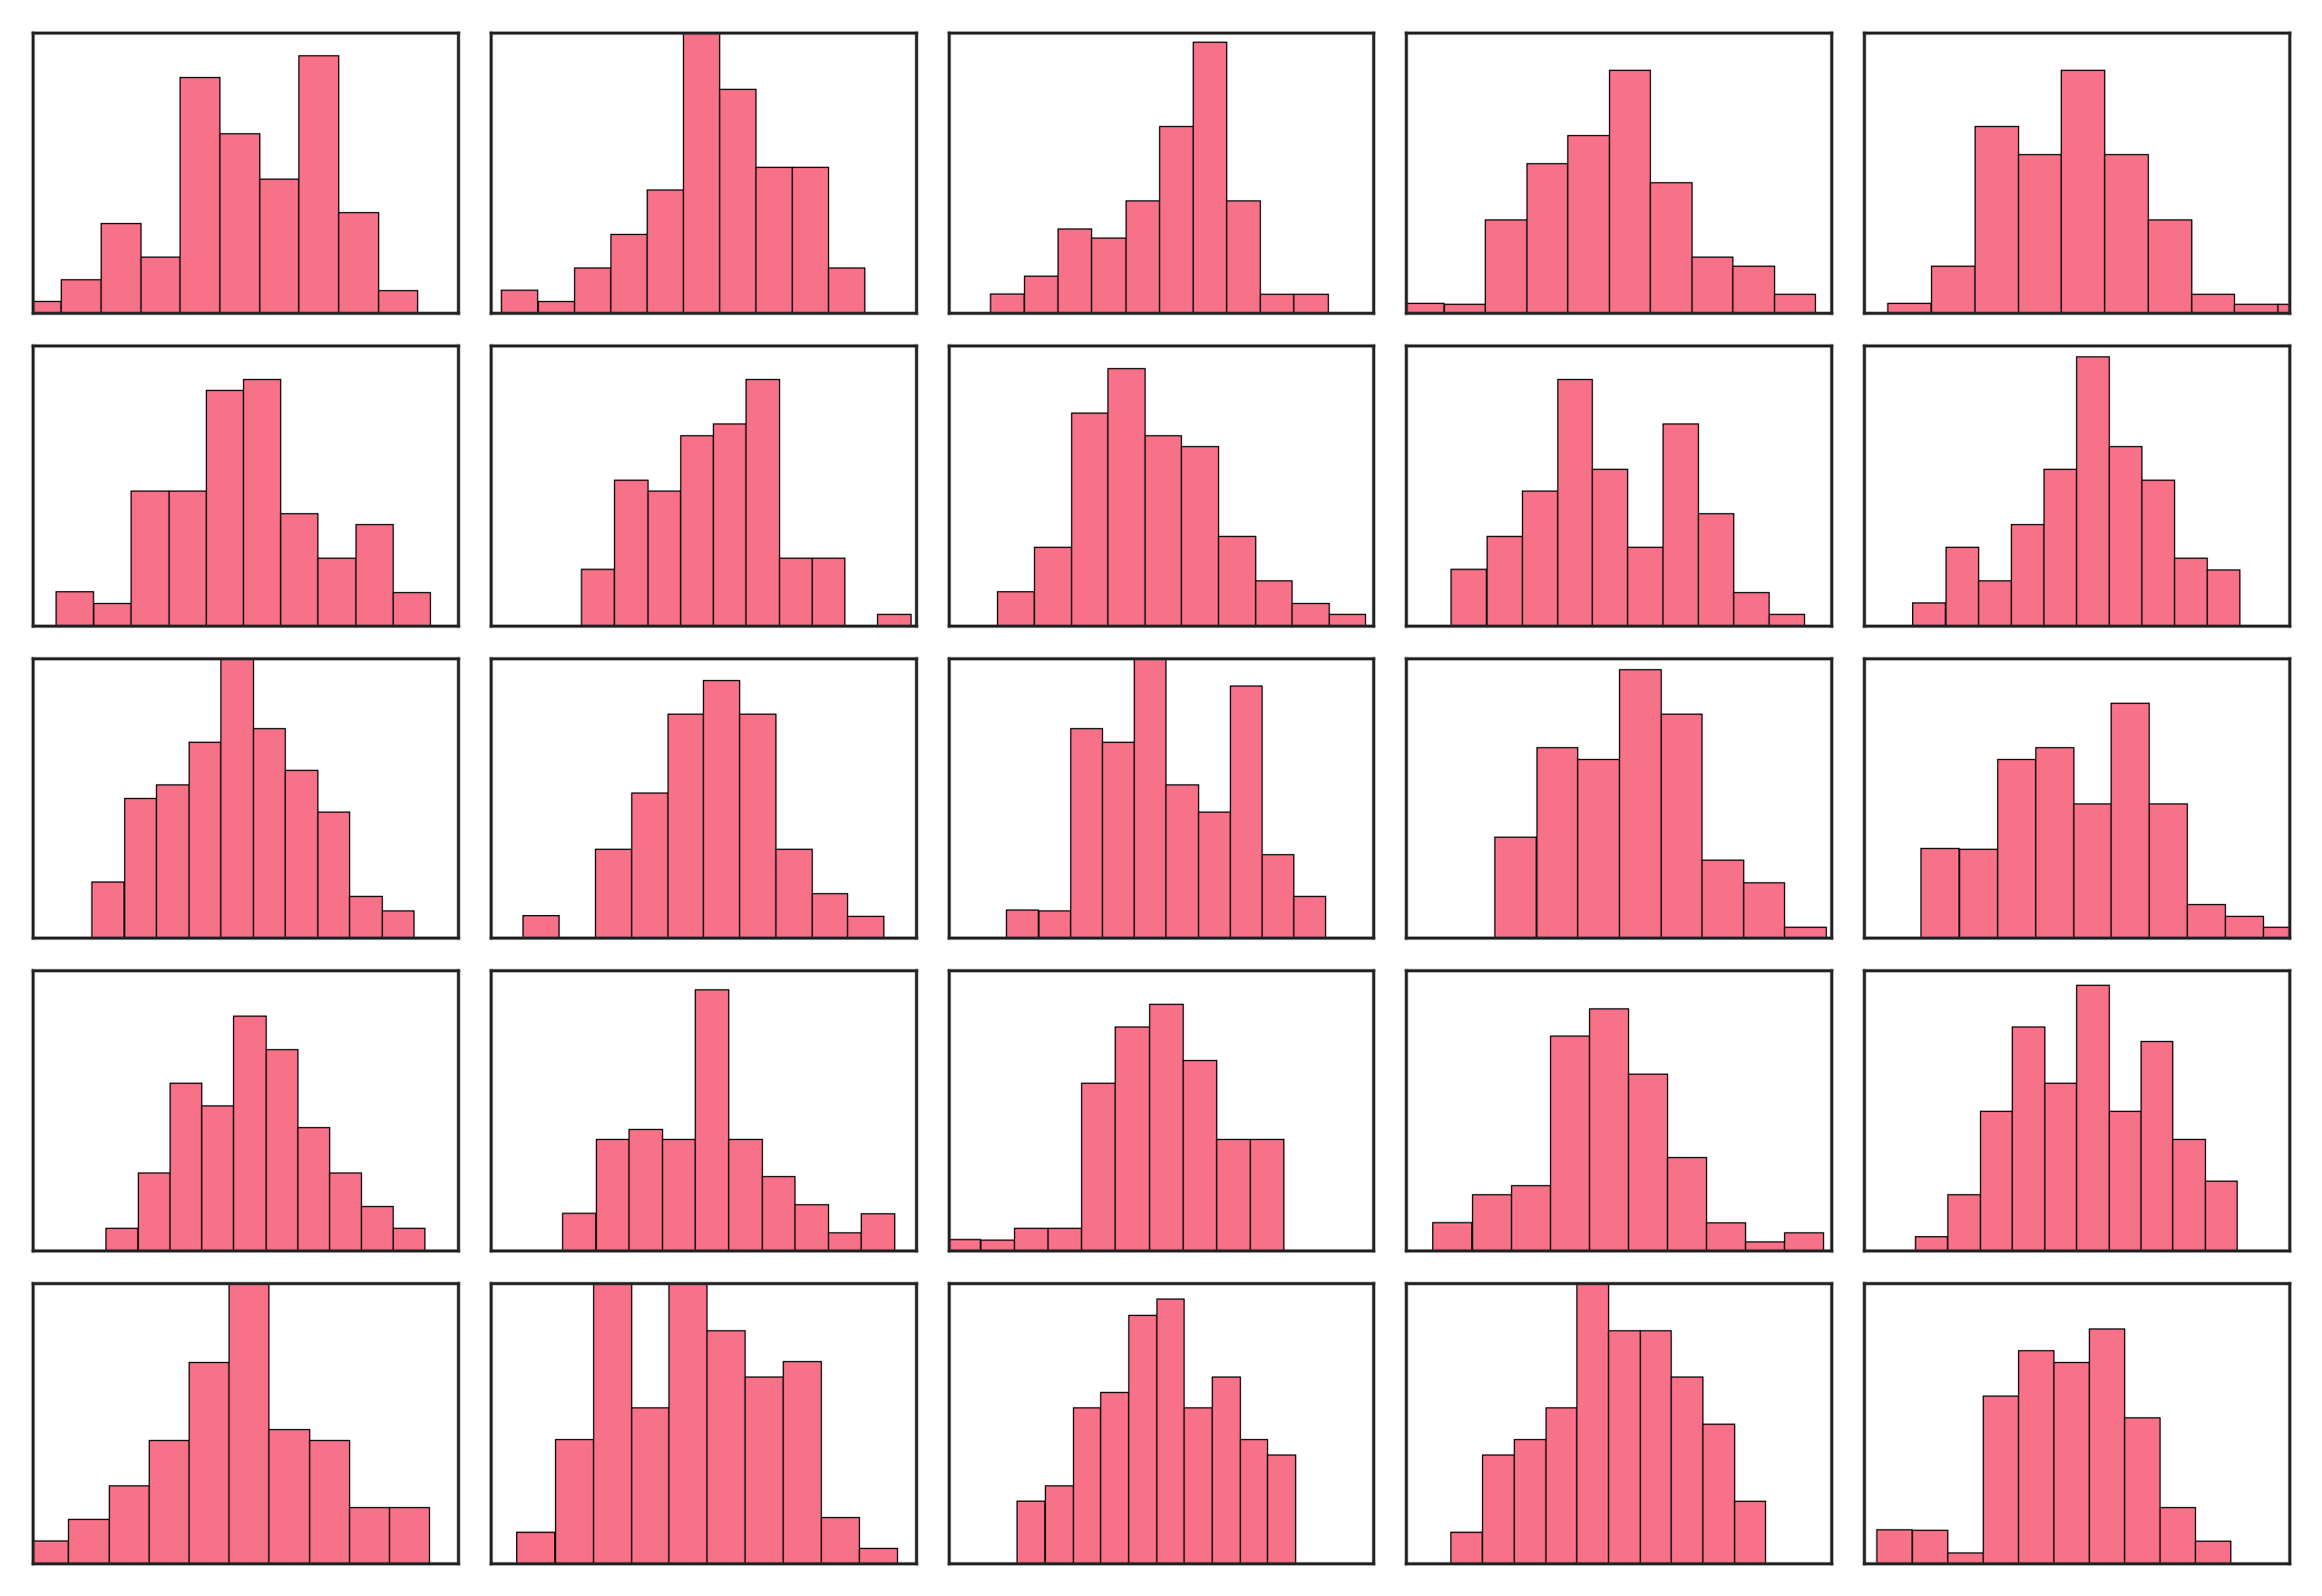
\includegraphics[width=0.75\textwidth]{../Images/Normal_MultHist.png}\\
  \caption{25 randomly generated normal distributions of 100 points.}\label{fig:MultipleNormal}
\end{figure}

The normal distribution with parameters $\mu$ and $\sigma$ is denoted as {$N(\mu,\sigma)$}. If the random variates (rvs) {\itshape X} are normally distributed with expectation $\mu$ and standard deviation $\sigma$, one writes: {$\,X \in N(\mu,\sigma)$}.

\begin{figure}
  \centering
  % Requires \usepackage{graphicx}
  \includegraphics[width=0.8\textwidth]{../Images/area_SDs.png}\\
  \caption{Area under +/1 1, 2, and 3 standard deviations of a normal distribution.}\label{fig:area_SDs}
\end{figure}

\begin{table}
  \centering
  \begin{tabular}{c c c}
    \hline
     & \multicolumn{2}{ c } {Probability of being} \\
    Range & within range & outside range \\
    \hline
    % after \\: \hline or \cline{col1-col2} \cline{col3-col4} ...
    mean $\pm$ 1SD & 0.683 & .317 \\
    mean $\pm$ 2SD & 0.954 & 0.046 \\
    mean $\pm$ 3SD & 0.9973 & 0.0027 \\
    \hline
  \end{tabular}
  \caption{Tails of a normal distribution.}
\end{table}

\vspace{5 mm}

\PyImg "distributionNormal.py" (p \pageref{py:distributionNormal}) shows simple manipulations of normal distribution functions.
\index{python}{distributionNormal}

\begin{lstlisting}[language=Python]
  In [1]:   import numpy as np
  In [2]:  from scipy import stats
  In [3]:  mu = -2
  In [4]:  sigma = 0.7
  In [5]:  myDistribution = stats.norm(mu, sigma)
  In [6]:  significanceLevel = 0.05
  In [7]:  myDistribution.ppf([significanceLevel/2, 1-significanceLevel/2])
  Out[8]:  array([-3.38590382, -0.61409618]
\end{lstlisting}

\emph{Example of how to calculate the interval of the PDF containing 95\% of the data, for the blue curve in Figure \ref{fig:normal}}

\subsubsection{Sum of Normal Distributions}\index{general}{normal distribution!sum of}

An important property of normal distributions is that the sum (or difference) of two normal distributions is also normally distributed. i.e., if

\begin{eqnarray*}
    X &\in& N(\mu_X, \sigma_X^2) \\
    Y &\in& N(\mu_Y, \sigma_Y^2) \\
    Z &=& X + Y,
\end{eqnarray*}

then

\begin{equation}\label{eq:sumOfGaussians}
    Z \in N(\mu_X + \mu_Y, \sigma_X^2 + \sigma_Y^2).
\end{equation}

\subsubsection{Examples of Normal Distributions}\index{general}{normal distribution!examples}

\begin{itemize}
    \item If the average man is 175 cm tall with a standard deviation of 6 cm, what is the probability that a man found at random will be 183 cm tall?
    \item If cans are assumed to have a standard deviation of 4 grams, what does the average weight need to be in order to ensure that the 99\% of all cans have a weight of at least 250 grams?
   \item If the average man is 175 cm tall with a standard deviation of 6 cm and the average woman is 168 cm tall with a standard deviation of 3 cm, what is the probability that a randomly selected man will be shorter than the randomly selected woman?
\end{itemize}

\subsection{Central Limit Theorem}\label{sec:CentralLimitTheorem}\index{general}{central limit theorem}
The central limit theorem states that the mean of a sufficiently large number of identically distributed random variates\index{general}{variate} will be approximately normally distributed. Or in other words, the sampling distribution of the mean tends toward normality, regardless of the distribution.
\ref{fig:CentralLimitTheorem} shows that averaging over 10 uniformly distributed data already produces a smooth, almost Gaussian distribution.

\begin{figure}
  \centering
  % Requires \usepackage{graphicx}
  \includegraphics[width=0.7\textwidth]{../Images/CentralLimitTheorem.png}\\
  \caption{Demonstration of the "Central Limit Theorem": Left) Histogram of random data between 0 and 1. Center) Histogram of average over two datapoints.) Right) Histogram of average over 10 datapoints.}\label{fig:CentralLimitTheorem}
\end{figure}

\PyImg "centralLimitTheorem.py" (p \pageref{py:centralLimitTheorem}) demonstrates that already averaging over 10 uniformly distributed datapoints produces an almost Gaussian distribution.
\index{python}{distributionDiscrete}

\subsection{Application Example}

To illustrate the ideas behind the use of distribution functions, let us go step-by-step through the analysis of the following problem:

The average weight of a newborn child in the US is 3.5 kg, with a standard deviation of 0.76 kg. If we want to check all children that are significantly different from the typical baby, what should we do with a child that is born with a weight of 2.6 kg?

\begin{itemize}
  \item Find the distribution that characterizes healthy babies ($\mu=3.5, \sigma=0.76$).
  \item Calculate the CDF at the interesting value (\emph{CDF(2.6 kg) = 0.118}).
  \item Interpret the result -see Fig. \ref{fig:pdf_checkValue} (\emph{"If the baby is healthy, the chance that its weight deviates by at least the observed value from the mean is 2*11.8\% = 23.6\% - This is not significant"}).
\end{itemize}

\begin{figure}
  \centering
  \includegraphics[width=0.75\textwidth]{../Images/pdf_checkValue.png}\\
  \caption{The chance that a healthy baby weighs 2.6 kg or less is 11.8\% (darker blue area). The chance that the difference from the mean is that much is twice that much, as the lighter blue area must be added.}\label{fig:pdf_checkValue}
\end{figure}

\section{Other Continuous Distributions}\label{sec:ContinuousDistributions} \index{general}{distributions!continuous}

Frequently encountered distributions are:

\begin{itemize}
  \item \textbf{Normal distribution} - the "ideal" continuous probability distribution.
  \item \textbf{t-distribution} - for sample distributions. (What you will probably use most frequently.)
  \item \textbf{$\chi$-square distribution} - for describing  variability.
  \item \textbf{F-distribution} - for comparing variability.
\end{itemize}

In the following, we will describe these distributions in more detail. Other distributions you should have heard about will be mentioned briefly:

\begin{itemize}
  \item \textbf{Lognormal distribution} - a normal distribution, plotted on an exponential scale. This transformation is often used to convert a strongly skewed distribution into a normal one.
  \item \textbf{Weibull distribution} - mainly used for reliability or survival data.
  \item \textbf{Exponential distribution} - exponential curves.
  \item \textbf{uniform distribution} - when everything is equally likely.
\end{itemize}

\subsubsection{t Distribution}\index{general}{distributions!t-distribution}

In 1908 W.S. Gosset, who worked for the Guinnes brewery in Dublin, was interested in the problems of small samples, for example the chemical properties of barley where sample sizes might be as low as 3. Since in these measurements the true variance of the mean was unknown, it must be approximated by the sample standard error of the mean. And the ratio between the sample mean and the standard error had a distribution that was unknown till Gosset, under the  pseudonym "Student", solved that problem.
The corresponding distribution is the t-distribution, and converges for larger values towards the normal distribution (Fig. \ref{fig:t}).

Since in most cases the population mean and its variance are unknown, one typically works with the t-distribution when analyzing sample data.

If $\bar{x}$ is the sample mean, and $s$ the sample standard deviation, then

\begin{equation}
  t = \frac{\bar{x}-\mu}{s/ \sqrt{n}}
\end{equation}\label{eq:Tdistribution}

A very frequent application of the t-distribution is in the calculation of confidence intervals for the mean. The width of the 95\%-confidence interval, i.e. the interval that contains the true mean with a chance of 95\%, is the same width about the population mean that contains 95\% of the sample means (Eq. \ref{eq:ci_t}):

\begin{equation}
  ci = mean \pm std * t_{df,\alpha}
\end{equation}\label{eq:ci_t}

The following example shows how to calculate the t-values for confidence intervals, for n = 20 and $\alpha=0.05$. For comparison, I also calculate the corresponding value from the normal distribution:

\begin{lstlisting}[language=Python]
  In [1]: from scipy import stats
  In [2]: n = 20
  In [3]: df = n-1
  In [4]: alpha = 0.05
  In [5]: stats.t(df).ppf(1-alpha/2)
  Out[6]: 2.093

  In [7]: stats.norm.ppf(1-alpha/2)
  Out[7]: 1.960
\end{lstlisting}


In \emph{Python}, the 95\% confidence interval for the mean can be obtained with a one-liner:

\begin{lstlisting}[language=Python]
    In [8]: alpha = 0.95
    In [9]: df = len(data)-1
    In [10]: ci = stats.t.interval(alpha, df, loc=mean(data), scale=stats.sem(data))
\end{lstlisting}

\begin{figure}
  \centering
  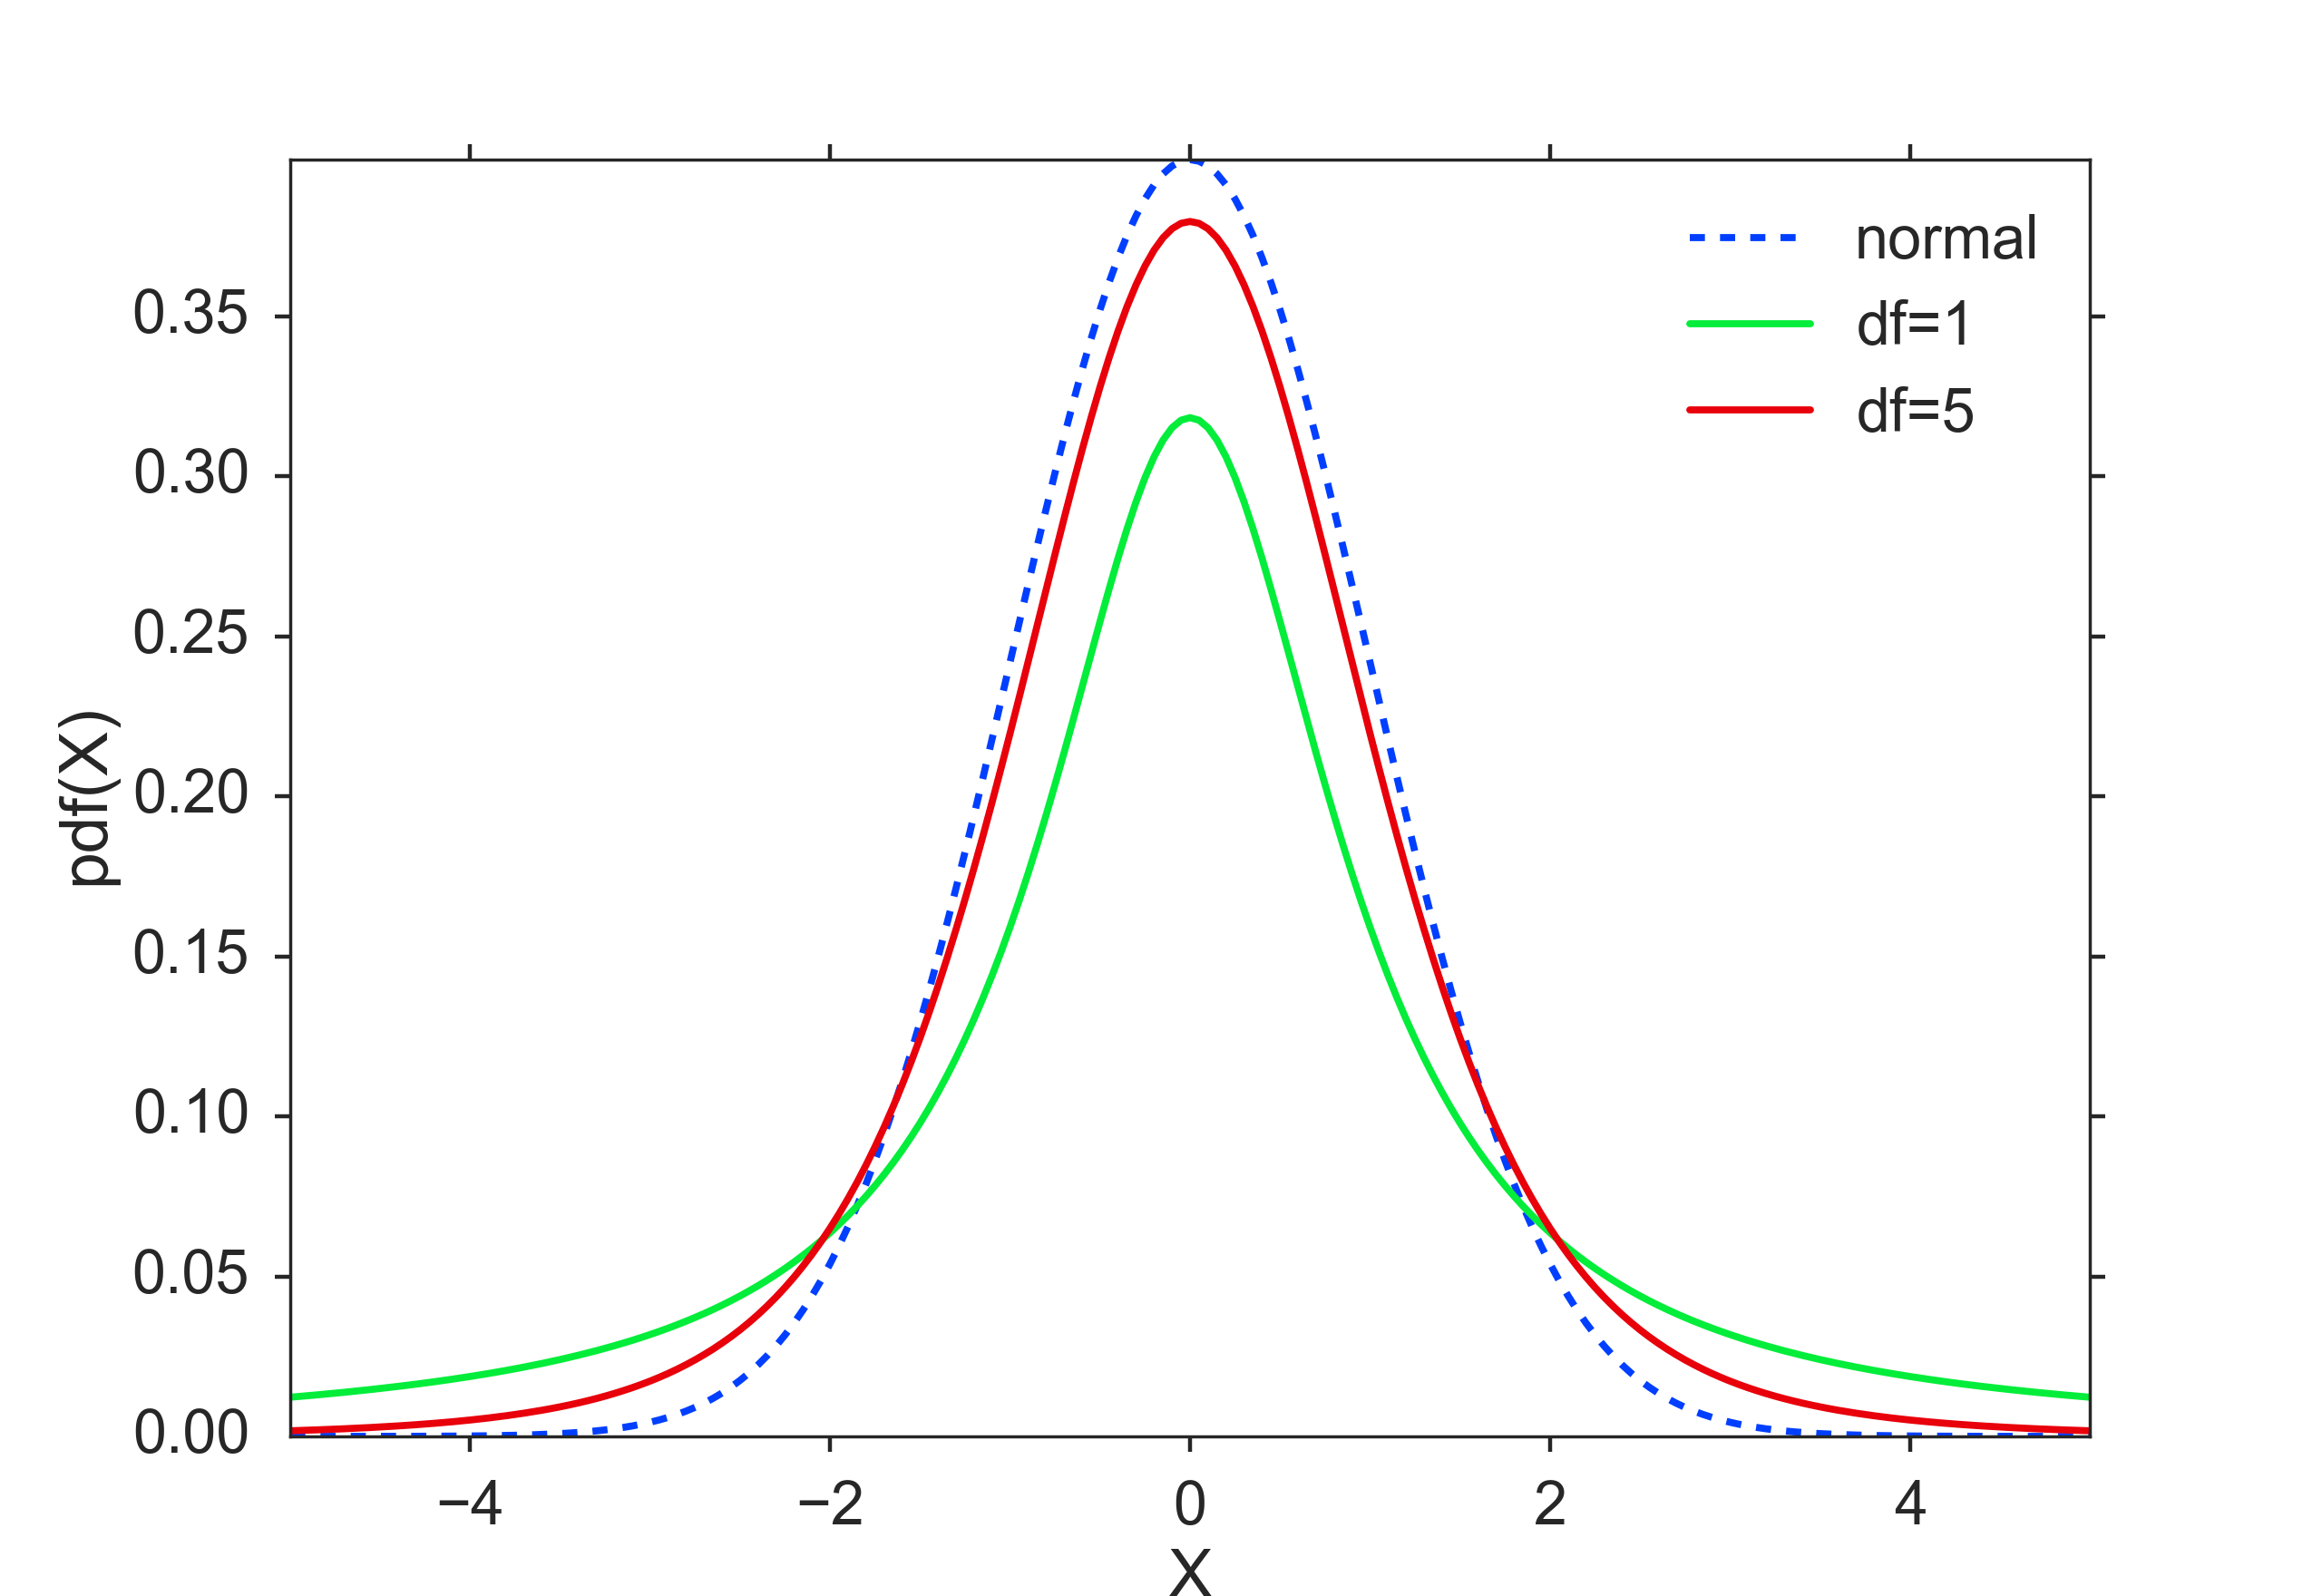
\includegraphics[width=0.5\textwidth]{../Images/dist_t.png}\\
  \caption{t Distribution}\label{fig:t}
\end{figure}

Since the t-distribution has longer tails than the normal distribution, it is much less affected by extreme cases (see Figure \ref{fig:ttest_stability}).

\begin{figure}
  \centering
  \includegraphics[width=0.75\textwidth]{../Images/ttest_stability.png}\\
  \caption{The t-distribution is much more robust against outliers than the normal distribution.}\label{fig:ttest_stability}
\end{figure}


\subsubsection{Chi-square Distribution}\index{general}{distributions!chi square}

The chi-square distribution is related to normal distribution in a simple way: If a random variable $X$ has a normal distribution ($X \in N(0,1)$), then $X^2$ has a chi-square distribution, with one degree of freedom ($X^2 \in \chi_{1}^2$). The sum squares of $n$ independent and standard normal random variables has a chi-square distribution with $n$ degrees of freedom (Fig. \ref{fig:chi2}):

\begin{equation}
    \sum\limits_{i = 1}^n {X_i^2} \in \chi_{n}^2
\end{equation}


\begin{figure}
  \centering
  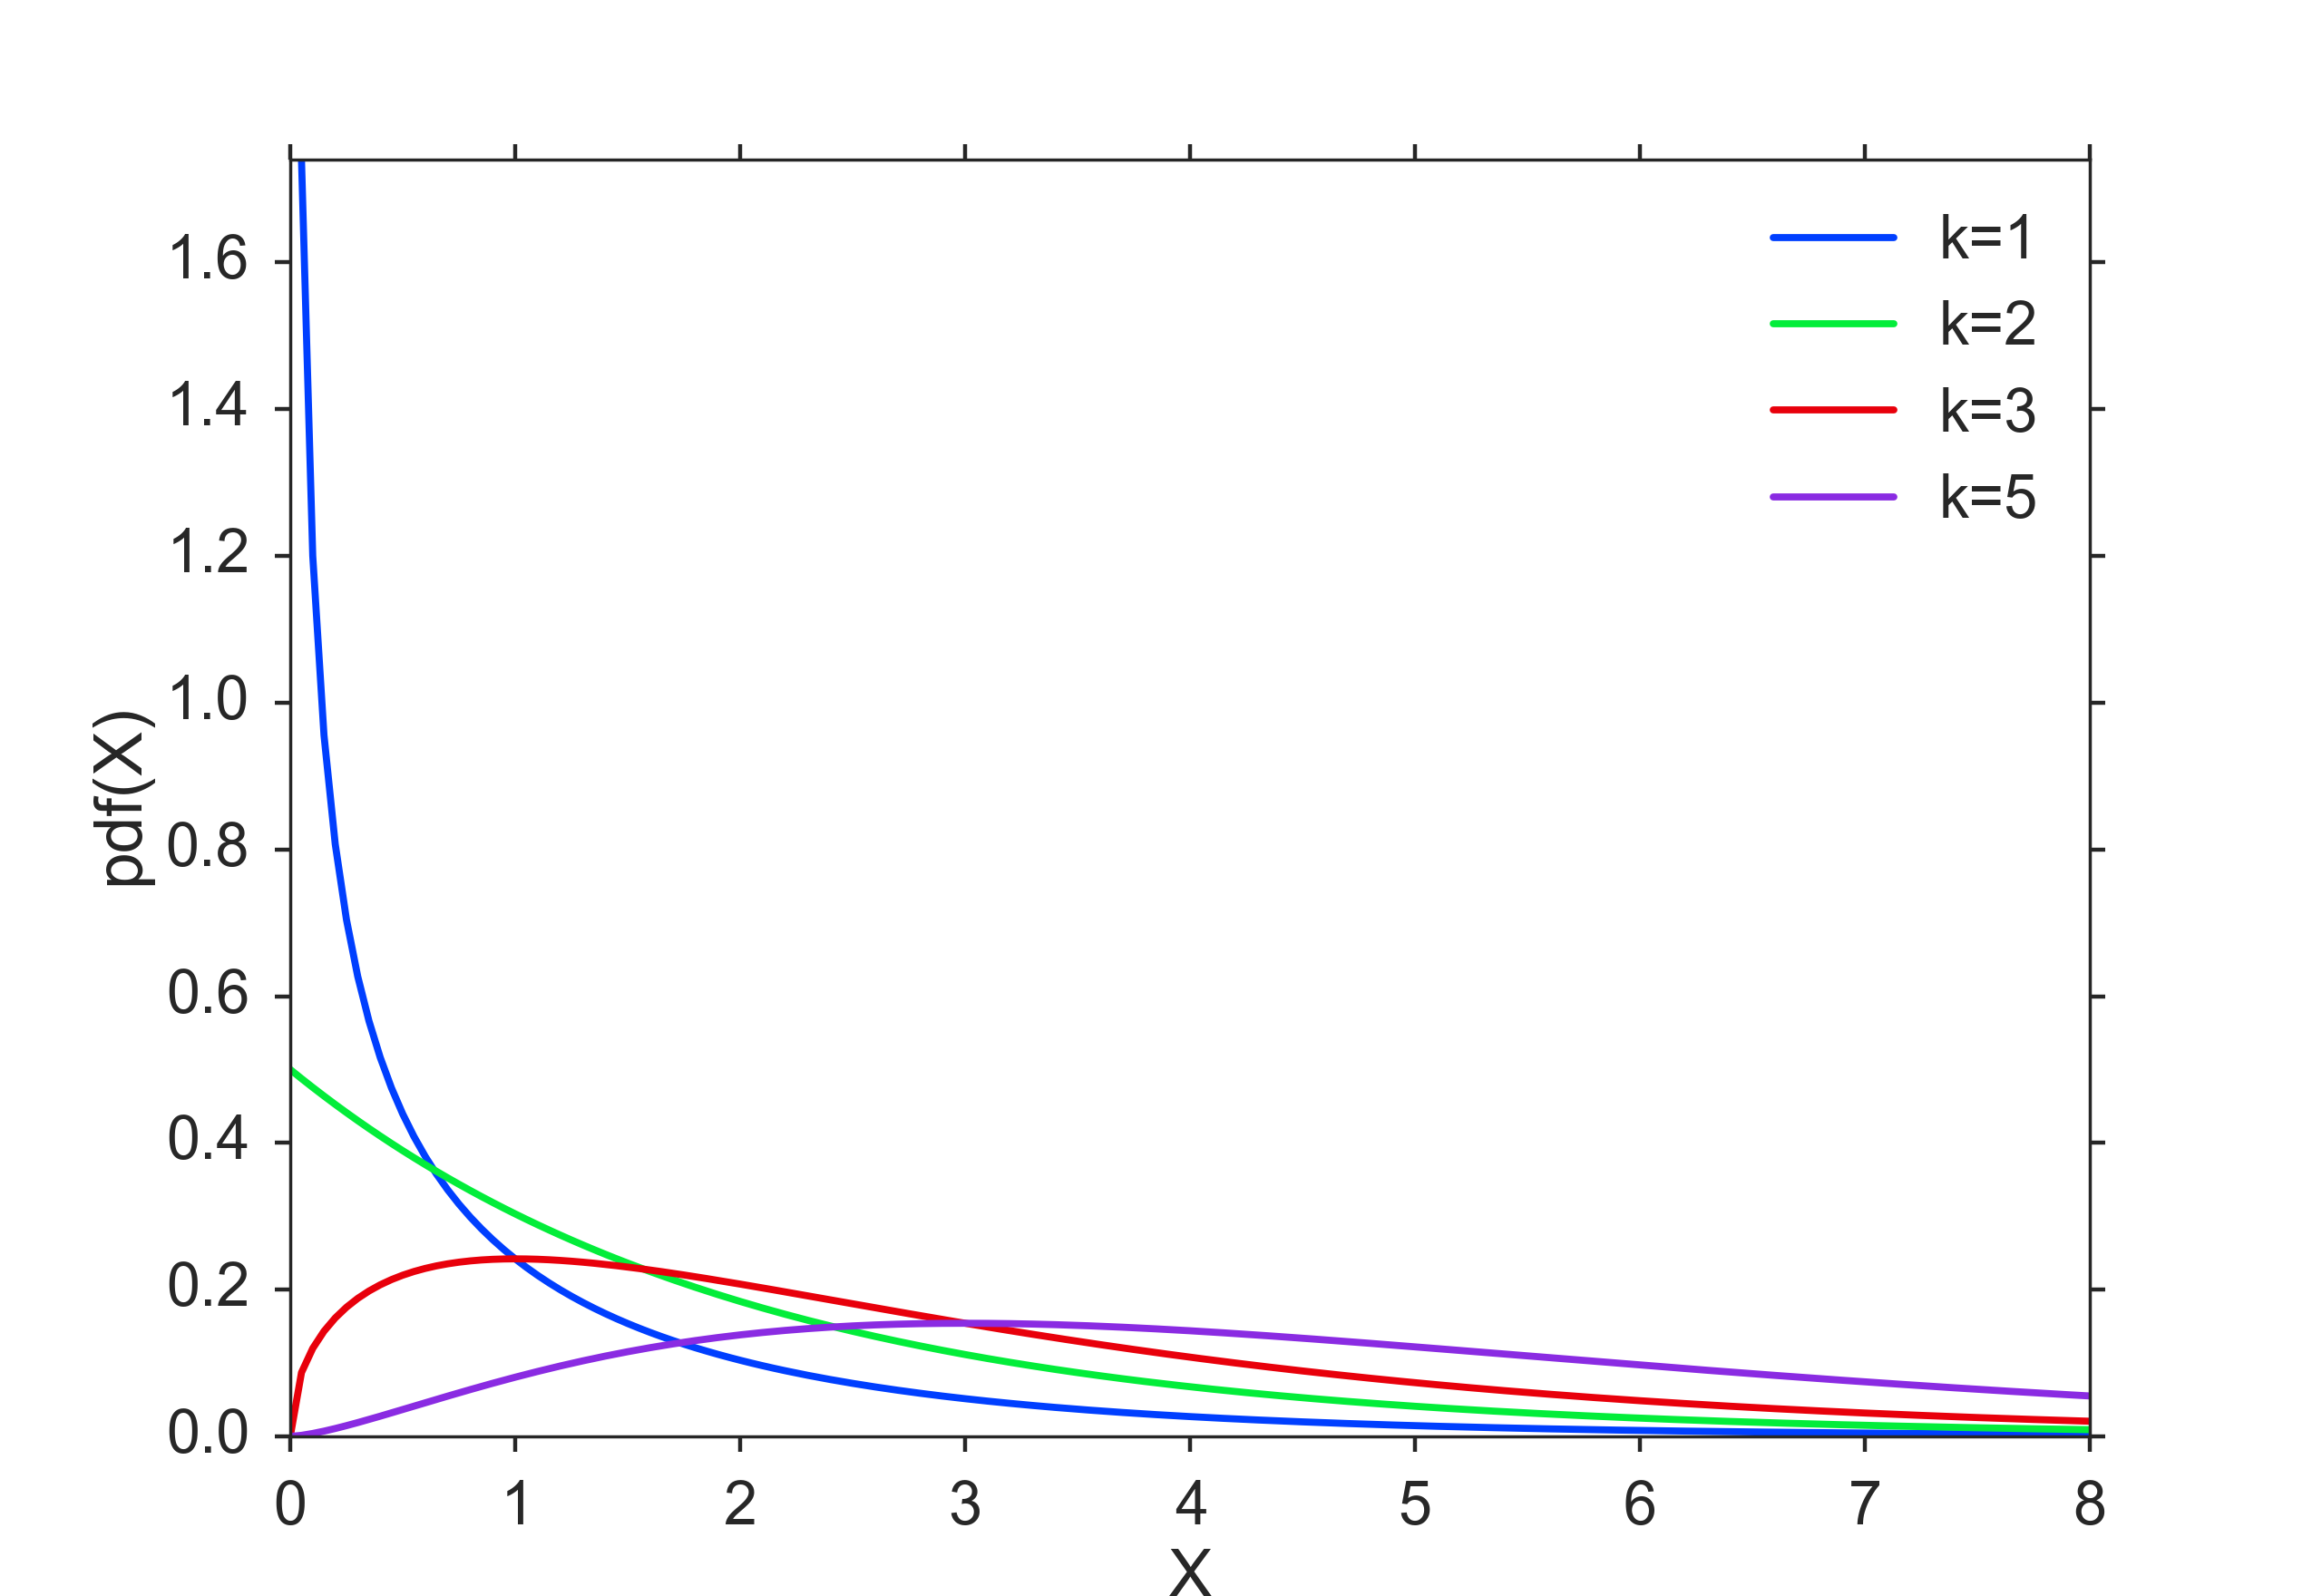
\includegraphics[width=0.5\textwidth]{../Images/dist_chi2.png}\\
  \caption{Chi-square Distribution}
  \label{fig:chi2}
\end{figure}

\textbf{Application Example}

A pill producer is ordered to deliver pills with a standard deviation of $\sigma=0.05$. From the next batch of pills you pick $n=13$ random samples. These samples $x_1, x_2, . . . , x_n$ have a weight of
3.04, 2.94, 3.01, 3.00, 2.94, 2.91, 3.02, 3.04, 3.09, 2.95, 2.99, 3.10, 3.02 g.

\emph{Question:} Is the standard deviation larger than allowed?

\emph{Answer:}

Since the chi-square distribution describes the distribution of the summed squares of random variates from a \emph{standard normal distribution}, we have to normalize our data before we calculate the corresponding CDF-value:

\begin{equation}
  1 - CD{F_{{\chi ^2}_{(n - 1)}}}\left( {\sum {(\frac{{x - \bar x}}{\sigma }} {)^2}} \right) = 0.1929
\end{equation}

\emph{Interpretation:} if the batch of pills is from a distribution with a standard deviation of $\sigma=0.05$, the likelihood of obtaining a chi-square value as large or larger than the one observed is about 19\%, so it is not atypical. In other words, the batch matches the expected standard deviation.

\subsubsection{F Distribution}\index{general}{distributions!F distribution}
Named after Sir Ronald Fisher, who developed the F distribution for use in determining critical values in ANOVAs ("ANalysis Of VAriance").
Suppose we want to calculate the variance of a variable in two separate subsets. "Is one more diverse than the other?" It is tempting to take the ratio of the variances, $S_1^2 / S_2^2$, but we don't know for sure how big or small that number must be before we conclude that the variances are different. This problem is solved by the F distribution. The cutoff values for an F distribution are found using three variables:

\begin{itemize}
  \item ANOVA numerator degrees of freedom
  \item ANOVA denominator degrees of freedom
  \item significance level
\end{itemize}

ANOVA compares the size of the variance between two different samples. This is done by dividing the larger variance over the smaller variance. The formula for the resulting F statistic is (Fig. \ref{fig:Fdistribution}):

\begin{equation}
    F(r_1, r_2) = \frac{\chi_{r1} ^2 /r_1}{\chi_{r2} ^2 /r_2}
\end{equation}

where $\chi_{r1}^2$ and $\chi_{r2}^2$ are the chi-square statistics of sample one and two respectively, and $r_1$ and $r_2$ are their degrees of freedom.

\begin{figure}
  \centering
  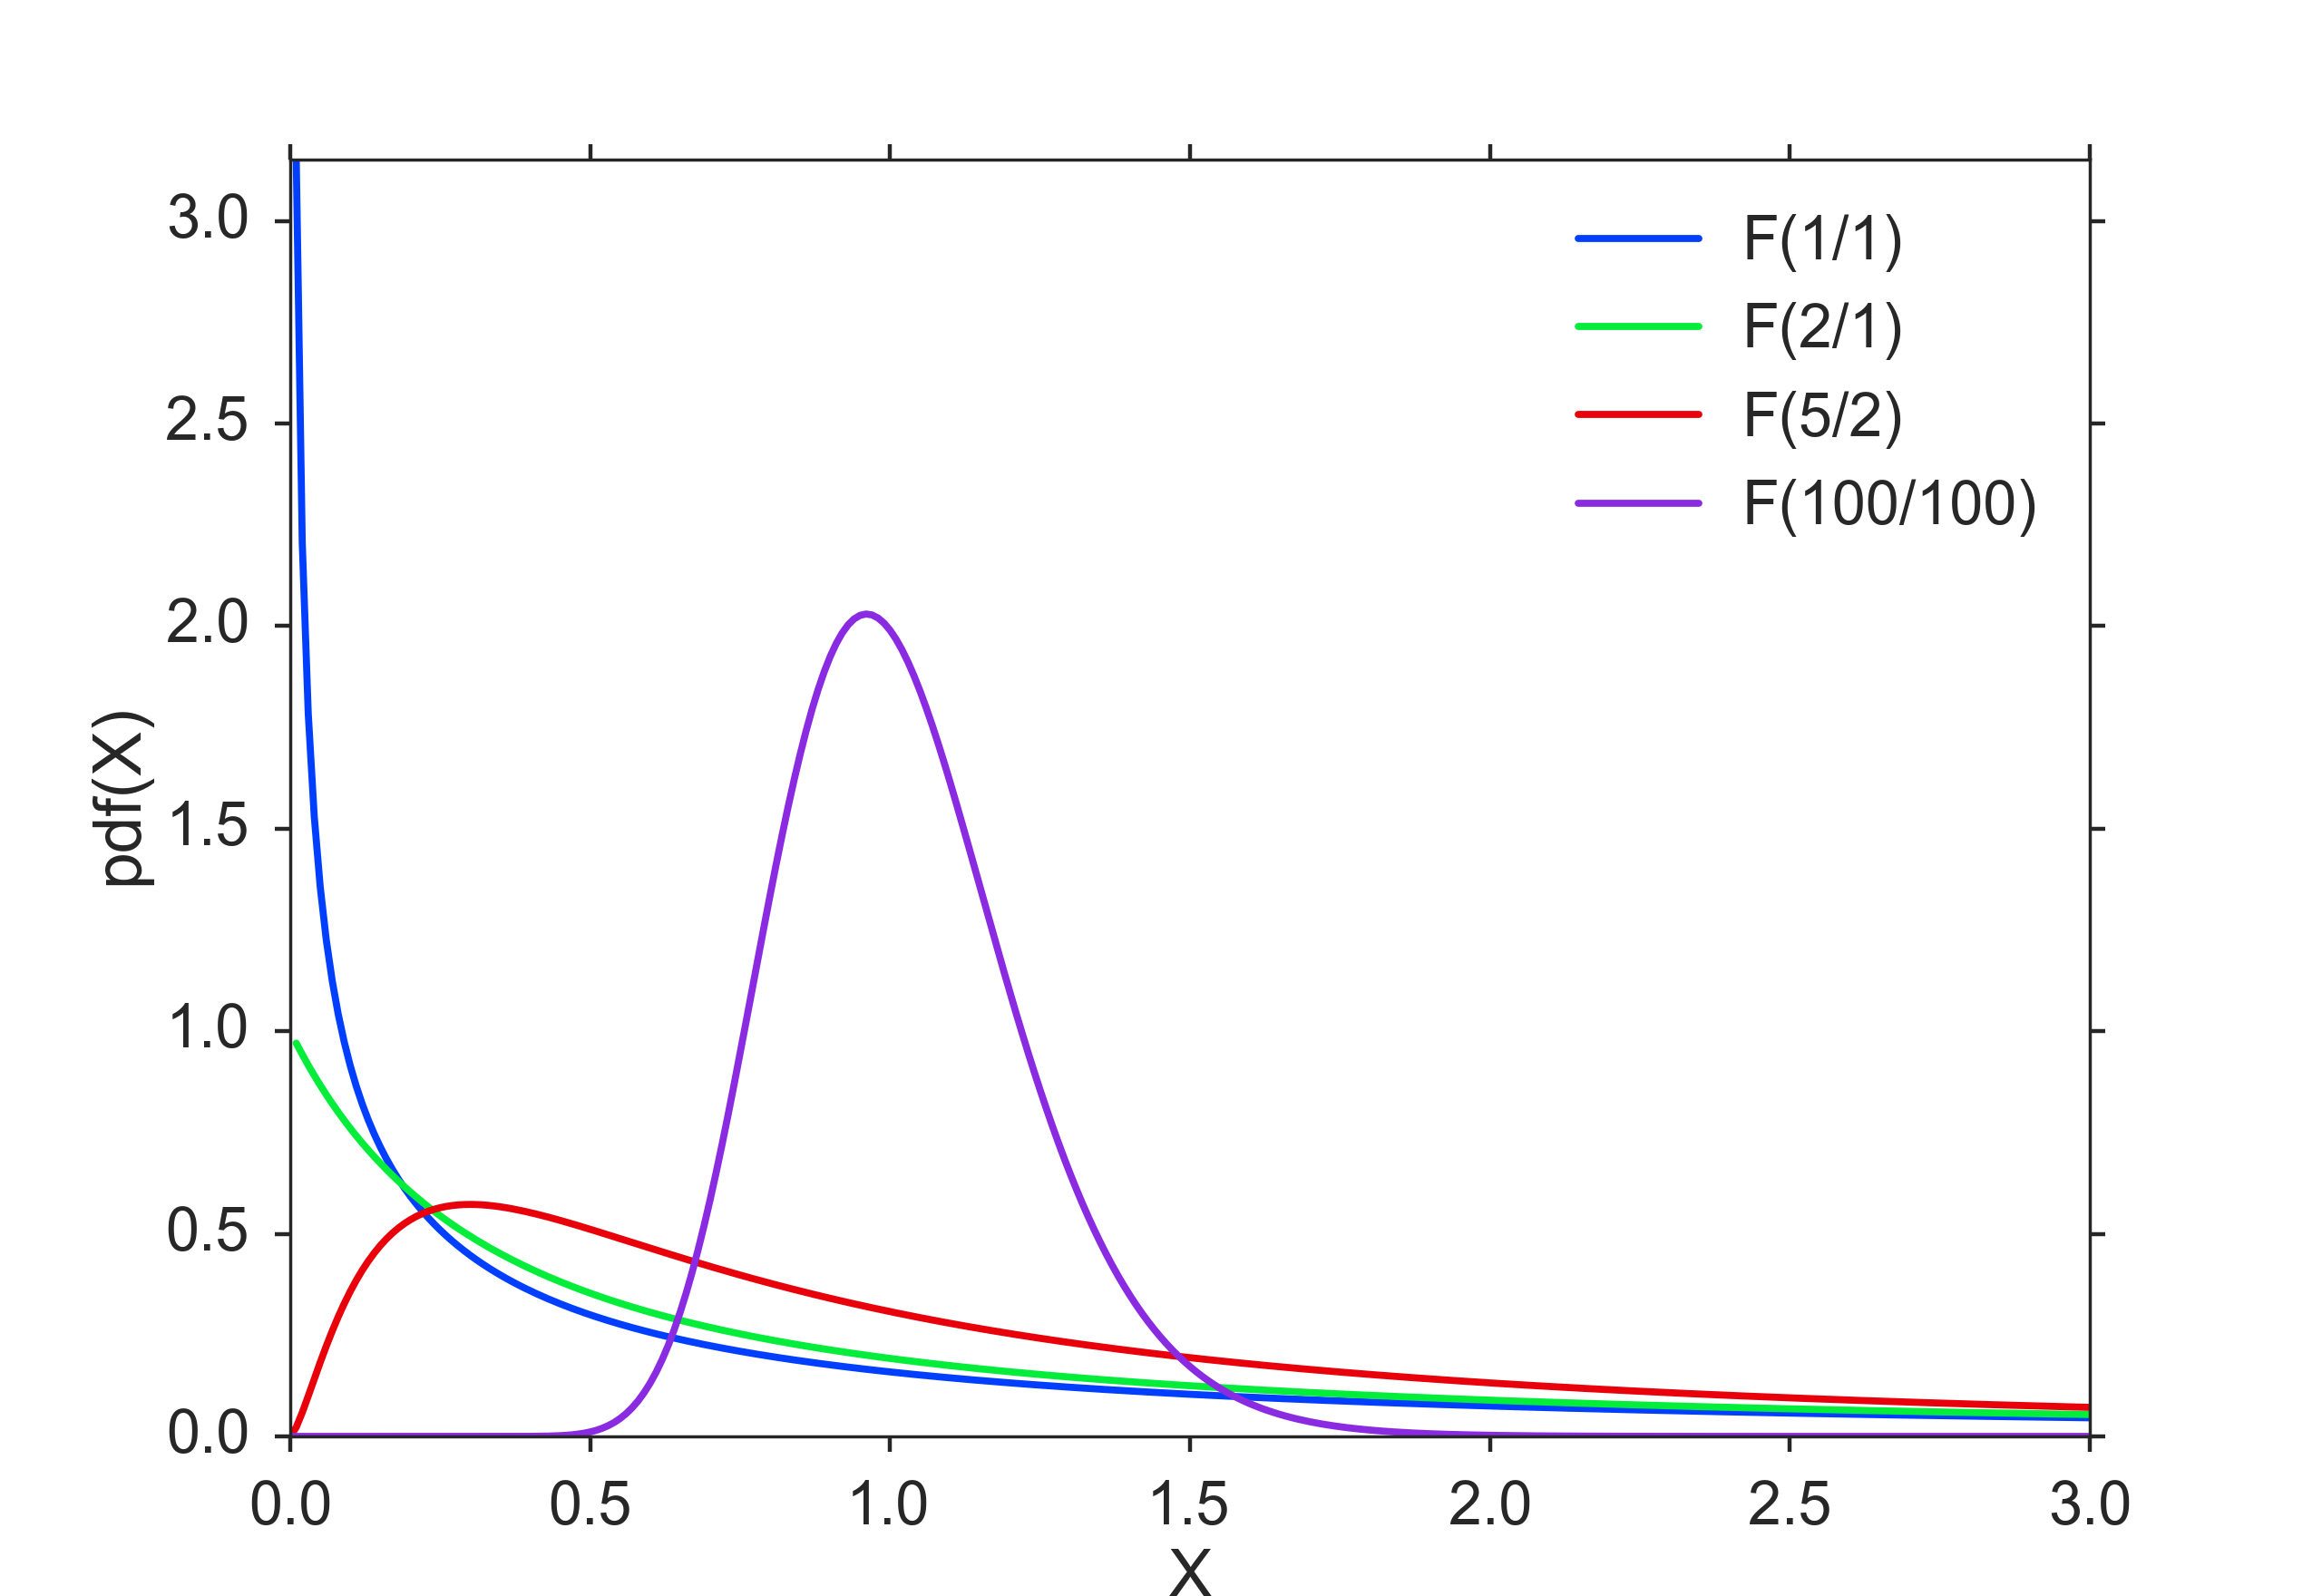
\includegraphics[width=0.5\textwidth]{../Images/dist_f.png}\\
  \caption{F Distribution}
  \label{fig:Fdistribution}
\end{figure}


\paragraph{F-Test of Equality of Variances}
If you want to investigate whether two groups have the same variance, you have to calculate the ratio of the sample standard deviations squared:

\begin{equation}
  F = \frac{S_x^2}{S_y^2}
\end{equation}

where $S_x$ ist he sample standard deviation of the first sample, and $S_y$ the sample standard deviation for the second sample.

\paragraph{Application Example}

Take for example the case that you want to compare two methods to measure eye movements. The two methods
can have different accuracy and different precision (Fig. \ref{fig:accuracy}). With your test you want to
determine if the precision of the two methods is equivalent, or if one
method is more precise than the other.

\begin{figure}
  \centering
  \includegraphics[width=0.5\textwidth]{../Images/Accuracy_and_precision.png}\\
  \caption{Accuracy and precision of a measurement are two different characteristics!}
  \label{fig:accuracy}
\end{figure}

When you look 20 deg to the right, you get the following results:
Method 1: [20.7,  20.3,  20.3,  20.3,  20.7,  19.9,  19.9,  19.9,  20.3,
        20.3,  19.7,  20.3]
Method 2: [ 19.7,  19.4,  20.1,  18.6,  18.8,  20.2,  18.7,  19. ]

The F statistic is $F = 0.494$, and has $n-1$ and $m-1$ degrees of freedom, where $n$ and $m$ are the number of recordings with each method. The code sample below shows that the F statistic is close to the center of the distribution, so we cannot reject the hypothesis that the two methods have the same precision.

\begin{lstlisting}[language=Python]
  In [1]: import numpy as np

  In [2]: method1 = np.array([20.7,  20.3,  20.3,  20.3,  20.7,  19.9,  19.9,  19.9,  20.3, 20.3,  19.7,  20.3])

  In [3]: method2 = np.array([ 19.7,  19.4,  20.1,  18.6,  18.8,  20.2,  18.7,  19. ])

  In [4]: fval = np.var(method1, ddof=1)/np.var(method2, ddof=1)

  In [5]: fd = stats.f(len(method2)-1,len(method2)-1)

  In [6]: p = fd.cdf(fval)

  In [7]: print(p)
  Out[7]: 0.041

  In [8]: if (p<0.025) or (p>0.975):
              print('There is a significant difference between the two distributions.')
\end{lstlisting}


\subsubsection{Lognormal Distribution}\index{general}{distributions!lognormal}

Normal distributions are the easiest ones to work with. In some circumstances a set of data with a positively skewed distribution can be transformed into a symmetric, normal distribution by taking logarithms. Taking logs of data with a skewed distribution will often give a distribution that is near to normal (see Figure \ref{fig:lognormal}).

\begin{figure}
\centering
\begin{subfigure}{.5\textwidth}
  \centering
  \includegraphics[width=.8\linewidth]{../Images/LogNormal_Linear.png}
  \caption{Plotted against a linear abscissa.}
  \label{fig:Lognormal_Sub1}
\end{subfigure}%
\begin{subfigure}{.5\textwidth}
  \centering
  \includegraphics[width=.8\linewidth]{../Images/LogNormal_Logarithmic.png}
  \caption{Plotted against a logarithmic abscissa.}
  \label{fig:Lognormal_Sub2}
\end{subfigure}
\caption{Lognormal distribution}
\label{fig:lognormal}
\end{figure}

\subsubsection{Weibull Distribution}\index{general}{distributions!weibull}\label{sec:Weibull}

The Weibull distribution is the most commonly used distribution for modeling reliability data or "survival" data. It has two parameters, which allow it to handle increasing, decreasing or constant failure-rates (see Figure \ref{fig:weibull}).
It is defined as

\begin{equation}\label{eq:weibull}
f_x (x) =
  \begin{cases}
    \frac{k}{\lambda}\left(\frac{x}{\lambda}\right)^{k-1}e^{-(x/\lambda)^{k}} & x\geq0 ,\\
    0 & x<0 ,
    \end{cases}
\end{equation}

where $k > 0$ is the shape parameter and $\lambda > 0$ is the scale parameter of the distribution. Its complementary cumulative distribution function is a stretched exponential function.

If the quantity $x$ is a "time-to-failure", the Weibull distribution gives a distribution for which the failure rate is proportional to a power of time. The shape parameter, k, is that power plus one, and so this parameter can be interpreted directly as follows:

\begin{itemize}
  \item  A value of $k < 1$ indicates that the failure rate decreases over time. This happens if there is significant "infant mortality", or defective items failing early and the failure rate decreasing over time as the defective items are weeded out of the population.

  \item  A value of $k = 1$ indicates that the failure rate is constant over time. This might suggest random external events are causing mortality, or failure.
  \item  A value of $k > 1$ indicates that the failure rate increases with time. This happens if there is an "aging" process, or parts that are more likely to fail as time goes on.
\end{itemize}

In the field of materials science, the shape parameter k of a distribution of strengths is known as the "Weibull modulus"\index{general}{Weibull modulus}.

\begin{figure}
  \centering
  \includegraphics[width=0.5\textwidth]{../Images/Weibull_PDF.png}\\
  \caption{Weibull Distribution}\label{fig:weibull}
\end{figure}


\subsubsection{Exponential Distribution}\index{general}{distributions!exponential}

For a stochastic variable X with an exponential distribution, the probability distribution function is:
\begin{equation}\label{eq_exponential}
f_x (x) =
  \begin{cases}
\lambda e^{- \lambda x}, & \mbox{if } x \ge 0 \\
0, & \mbox{if } x < 0
\end{cases}
\end{equation}

The exponential PDF is shown in Figure \ref{fig:exponential}
\begin{figure}
  \centering
  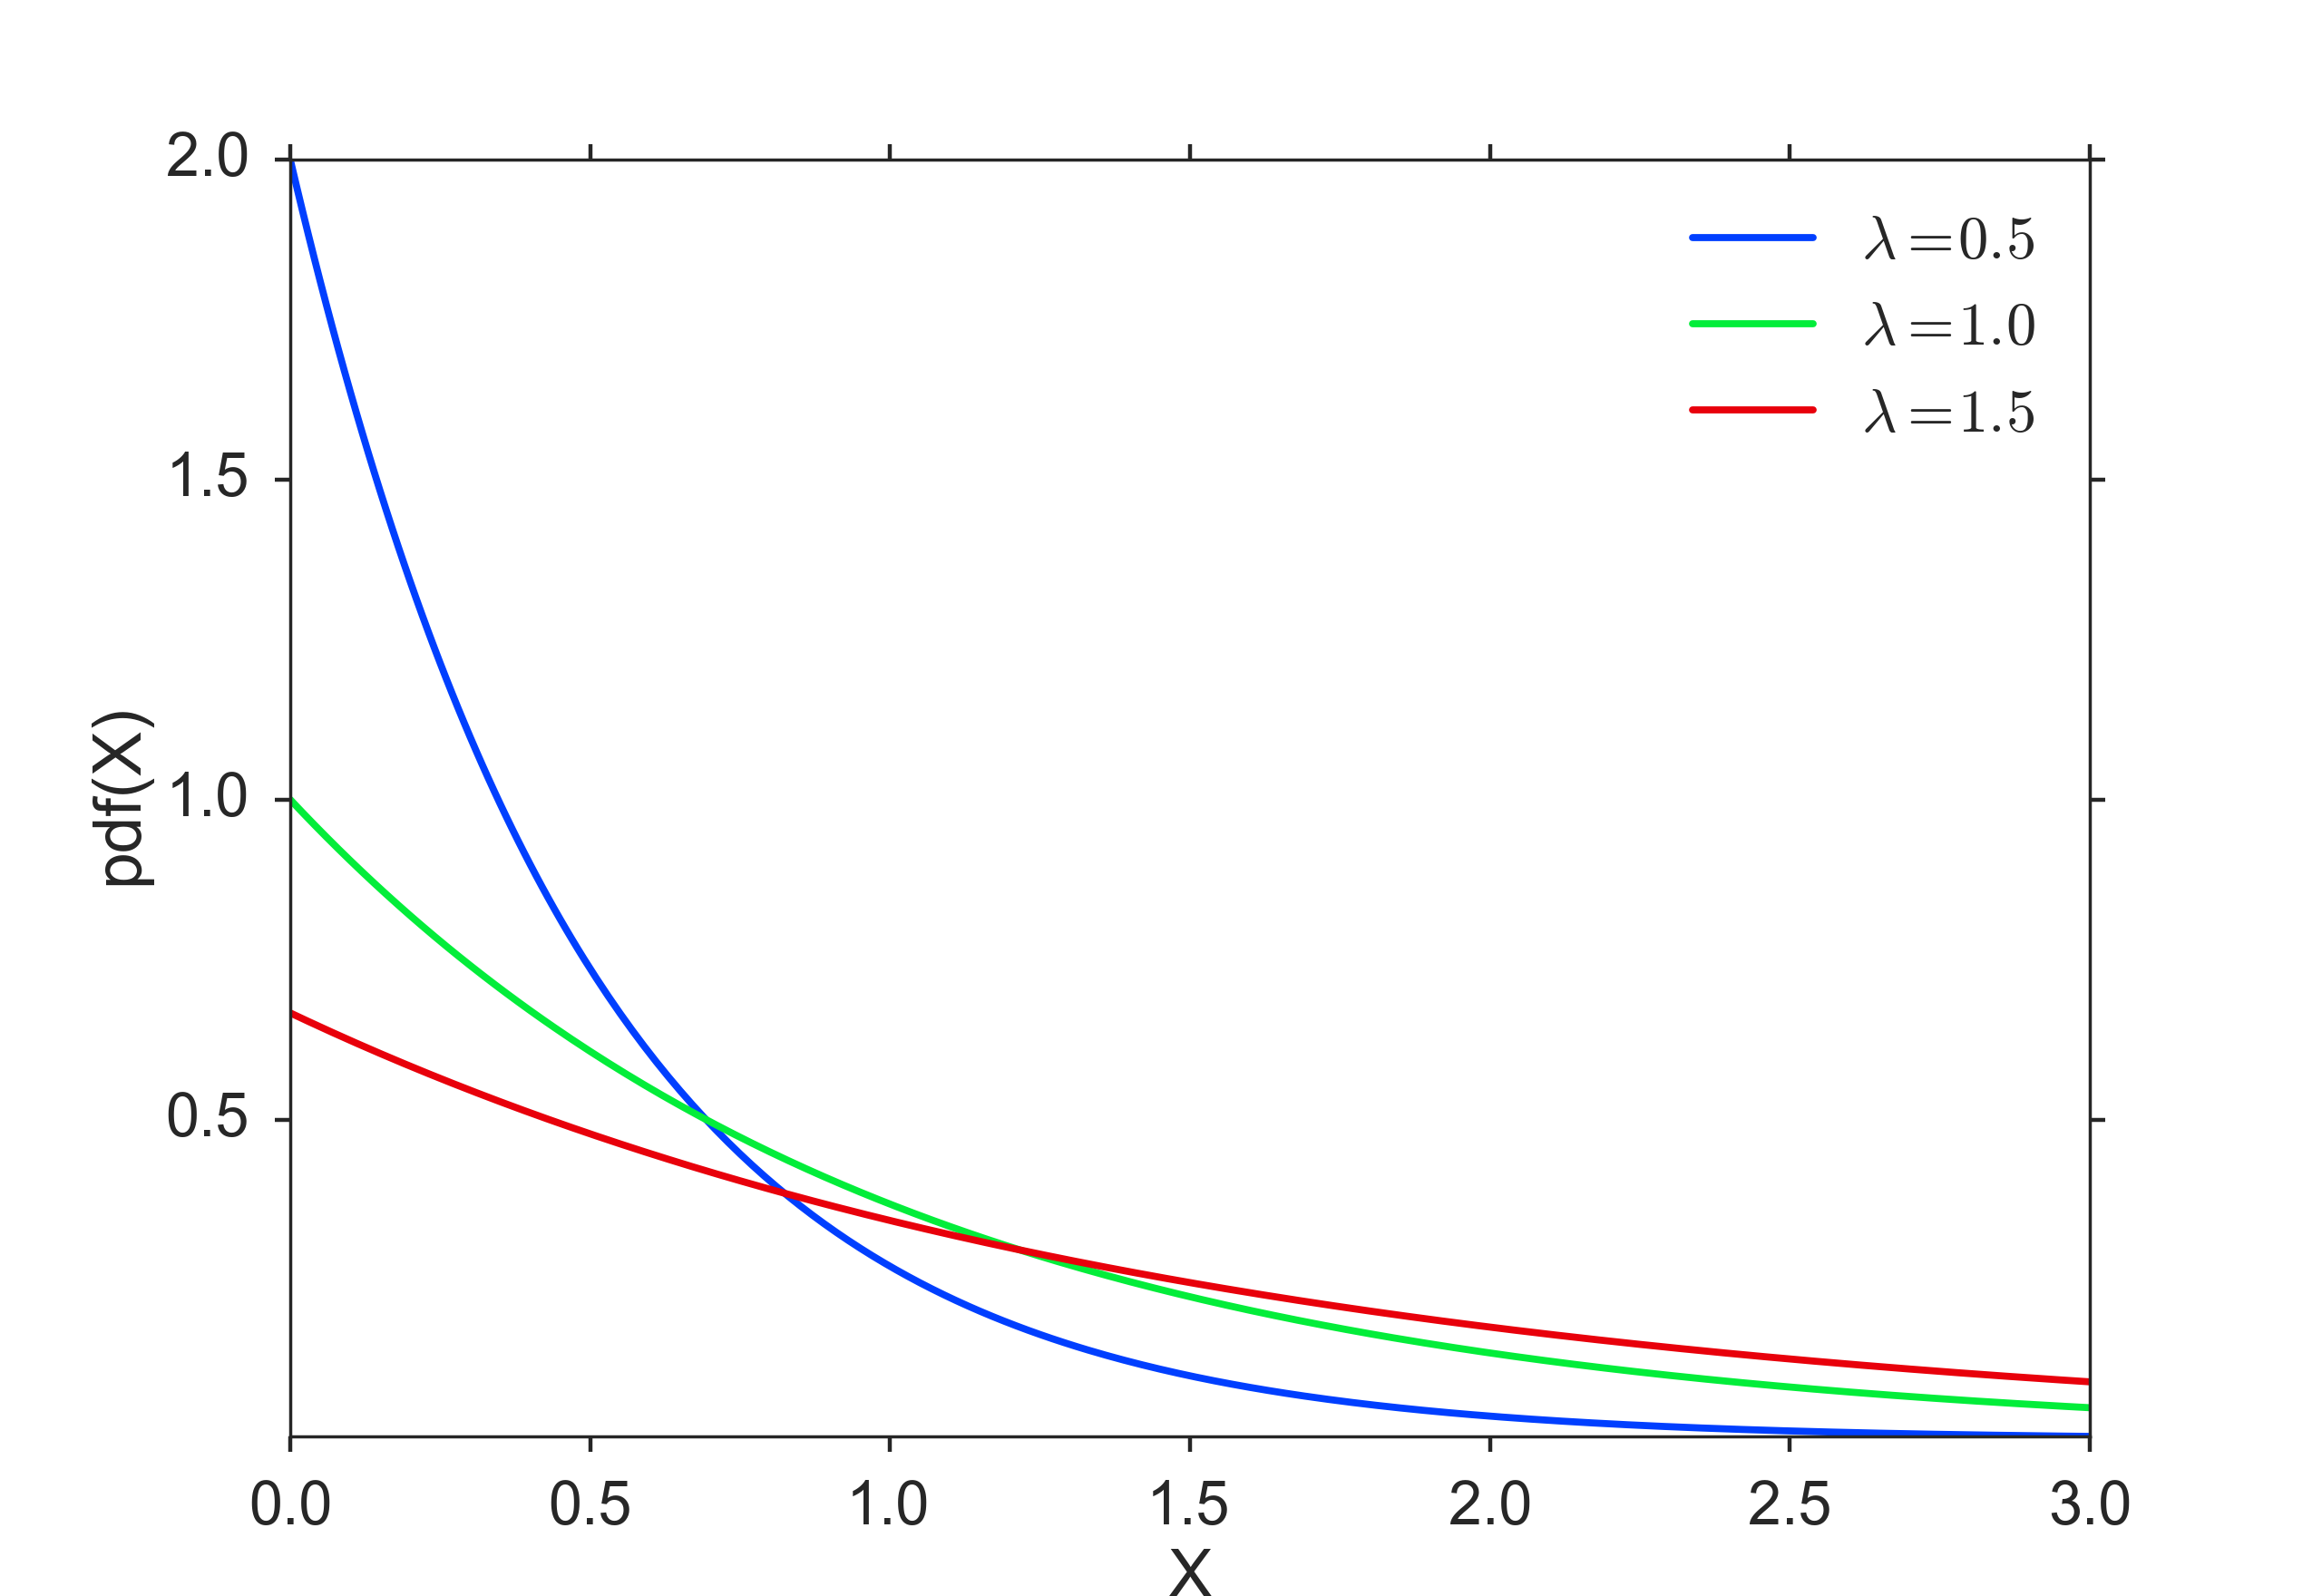
\includegraphics[width=0.5\textwidth]{../Images/dist_exp.png}\\
  \caption{Exponential Distribution}\label{fig:exponential}
\end{figure}


\subsubsection{Uniform Distribution}\index{general}{distributions!uniform}

This is a simple one: an even probability for all data values (Figure \ref{fig:uniform}). Not very common for real data.

\begin{figure}
  \centering
  \includegraphics[width=0.5\textwidth]{../Images/Uniform_Distribution_PDF.png}\\
  \caption{Uniform Distribution} \label{fig:uniform}
\end{figure}

\subsubsection{Programs: Continuous Distribution Functions}

\PyImg "distributionContinuous.py" (p \pageref{py:continuous}) shows different continuous distribution functions.
\index{python}{distributionContinuous}

\section{Exercises}

\subsection*{Python}
\begin{enumerate}
  \item Create an numpy-array, containing the data 1,2,3,...,10. Calculate mean and sample(!)-standard deviation.
    (Correct answer: 3.03)
\end{enumerate}

\subsection*{Distributions}


\begin{enumerate}
  \item  Generate and plot the Probability Density Function (PDF) of a normal distribution, with a mean of 5 and a standard deviation of 3.
  \item  Generate 1000 random data from this distribution.
  \item  Calculate the standard error of the mean of these data.
    (Correct answer: ca. 0.096)

  \item  Plot the histogram of these data.
  \item  From the PDF, calculate the interval containing 95\% of these data.
    (Correct answer: [ -0.88, 10.88])
\end{enumerate}

\subsection*{Continuous Distributions }
\begin{enumerate}
    \item \textbf{Normal Distribution:} Your doctor tells you that he can use hip implants for surgery even if they are 1 mm bigger or smaller than the specified size. And your financial officer tells you that you can discard 1 out of 1000 hip implants, and still make a profit.

        What is the required standard deviation for the producer of the hip implants, to simultaneously satisfy both requirements?
        (Correct answer: $\sigma=0.304 mm$)
    \item \textbf{T-Distribution:} Measuring the weight of your colleagues, you have obtained the following weights: 52, 70, 65, 85, 62, 83, 59 kg.
    Calculate the corresponding mean, and the 99\% confidence interval for the mean. Note: with n values you have n-1 DOF for the t-distribution.
    (Correct answer: 68.0 +/- 17.2 kg)

    \item \textbf{Chi-square Distribution:} Create 3 normally distributed datasets (mean = 0, SD = 1), with 1000 samples each. Then square them, sum them (so that you have 1000 data-points), and create a histogram with 100 bins. This should be similar to the curve for the Chi-square distribution, with 3 DOF (i.e. it should come down at the left, see figure below).
    \begin{figure}
      \centering
      \includegraphics[width=0.5\textwidth]{../Images/chi2_3dof.png}\\
      \caption{chi2 distribution with 3 degrees of freedom.}\label{fig:chi23dof}
    \end{figure}

    \item \textbf{F Distribution:} You have two apple trees. There are three apples from the first tree that weigh 110, 121 and 143 grams respectively, and four from the other which weigh 88, 93, 105 and 124 grams respectively. Are the variances from the two trees different?
    Note: calculate the corresponding F-value, and check if the CDF for the corresponding F-distribution is $<0.025$.
    (Correct answer: no)
\end{enumerate}
\subsection*{Discrete Distributions }

\begin{enumerate}

    \item Under which conditions do you use the binomial distribution to evaluate the likelihood of a discrete number of events? And under which do you use the Poisson distribution?

    \item \textbf{Binomial Distribution} "According to research, pure blue eyes in Europe approach greatest frequency in Finland, Sweden and Norway(at 72\%), followed by Estonia, Denmark(69\%); Latvia, Ireland(66\%); Scotland(63\%); Lithuania(61\%); The Netherlands(58\%); Belarus, England(55\%); Germany(53\%); Poland, Wales(50\%); Russia, The Czech Republic(48\%); Slovakia(46\%); Belgium(43\%); Austria, Switzerland, Ukraine(37\%); France, Slovenia(34\%); Hungary(28\%); Croatia(26\%); Bosnia and Herzegovina(24\%); Romania(20\%); Italy(18\%); Serbia, Bulgaria(17\%); Spain(15\%); Georgia, Portugal(13\%); Albania(11\%); Turkey and Greece(10\%). Further analysis shows that the average occurrence of blue eyes in Europe is 34\%, with 50\% in Northern Europe and 18\% in Southern Europe."

    If we have 15 Austrian students in the class-room, what ist the chance of finding 3, 6, or 10 students with blue eyes?
    (Correct answer: 9\%, 20.1\%, and 1.4\%)

    \item \textbf{Poisson Distribution} On the streets of Austria there were 62 fatal accidents in 2012. Assuming that those are evenly distributed, we have on average
    62 /(365/7)=1.19 fatal accidents per week. How big is the chance that in a given week there are no, 2, or 5 accidents?
    (Correct answer: 30.5\%, 21.5\%, 0.6\% )
\end{enumerate}

\chapter{Statistical Data Analysis}

\section{Typical Analysis Procedure}

In "the old days" (before computers with almost unlimited computational power were available), the statistical analysis of data was typically restricted to hypothesis tests: you formulate a hypothesis, collect your data, and then accept or reject the hypothesis. The resulting hypothesis tests form the basic framework for by far most analyses in  medicine and life sciences, and the most important hypotheses tests will be described in the following chapters.

The advent of powerful computers has changed the game. Nowadays, the analysis of statistical data is (or at least should be) a highly interactive process: you look at the data, and generate models which may explain your data. Then you determine the best fit parameters for these models, and check these models, typically by looking at the residuals. If you are not happy with the results, you modify the model to improve the correspondence between models and data; when you are happy, you calculate the confidence interval for your model parameters, and form your interpretation based on these values. An introduction into this type of statistical analysis is provided in chapter \ref{chapter:Models}.

In either case, one should start off with the following steps:
\begin{itemize}
  \item Visually inspect the data.
  \item Find extreme samples, and check them carefully.
  \item Determine the data-type of the values.
  \item If the data are continuous, check whether or not they are normally distributed.
  \item Select and apply the appropriate test, or start with the model-based analysis of the data.
\end{itemize}

\subsection{Data Screening}

The first step in data analysis is the visual inspection of the data. Our visual system is enormously powerful, and if the data are properly displayed, trends that characterize the data can be clearly visible. In addition to checking if the first and the last data values have been read in correctly, it is recommendable to check for missing data and outliers.

\subsubsection{Outliers} \index{general}{outliers}

There is no unique definition for outliers. However, for normally distributed samples they are often defined as data that lie either more than 1.5*IQR (inter-quartile range), or more than 2 standard deviations, from the sample mean. Outliers often fall in one of two groups: they are either caused by mistakes in the recording, in which case they should be excluded; or they constitute very important and valuable data points, in which case they have to be included in the data analysis. To decide which of the two is the case, you have to check the underlying raw data (for saturation or invalid data values), and the protocols from your experiments (for mistakes that may have occurred during the recording). If an underlying problem is detected, then - and only then - one may eliminate the outliers from the analysis. In every other case, the data have to be kept!

\subsection{Normality Check} \index{general}{normality check}

Statistical hypothesis tests can be grouped into parametric tests\index{general}{parametric tests} and non-parametric tests\index{general}{non-parametric tests}. Parametric tests assume that the data can be well described by a distribution that is defined by one or more parameters, in most cases by a normal distribution. For the given data set, the best-fit parameters for this distribution are then determined, together with their confidence intervals, and interpreted.

However, this approach only works if the given data set is in fact well approximated by the chosen distribution. If not, the results of the parametric test can be completely wrong. In that case non-parametric tests have to be used which are less sensitive, but therefore do not depend on the data following a specific distribution.

\begin{figure}
  \centering
  \includegraphics[width=0.75\textwidth]{../Images/ProbPlot.png}\\
  \caption{Probability-Plot, to check for normality of distribution.}\label{fig:qqplot}
\end{figure}


\subsubsection{Probability-Plots}\index{general}{plots!probability plot} \index{general}{plots!probplot}

In statistics, different tools are available for the visual assessments of distributions. They are graphical methods for comparing two probability distributions by plotting their \glspl{quantile}, or closely related parameters, against each other:

\begin{description}
  \item[QQ-Plots] \index{general}{plots!qq-plot}The "Q" in \acrfull{qq-plot} stands for \emph{quantile}. The quantiles of a given data set are plotted against the quantiles of a reference distribution, typically the standard normal distribution.
  \item[PP-Plots] \index{general}{plots!pp-plot} Plot the CDF (cumulative-distribution-function) of a given data set against the CDF of a reference distribution.
  \item[Probability Plots] \index{general}{plots!probability plot} Plot the ordered values of a given data set against the quantiles of a reference distribution.
\end{description}

In all three cases the results are similar: if the two distributions being compared are similar, the points will approximately lie on the line $y = x$. If the distributions are linearly related, the points will approximately lie on a line, but not necessarily on the line $y = x$ (Figure \ref{fig:qqplotChi2}).

In \emph{Python}, the plot can be generated with the command

\begin{lstlisting}[language=Python]
    stats.probplot(data, plot=plt)
\end{lstlisting}

\begin{figure}
  \centering
  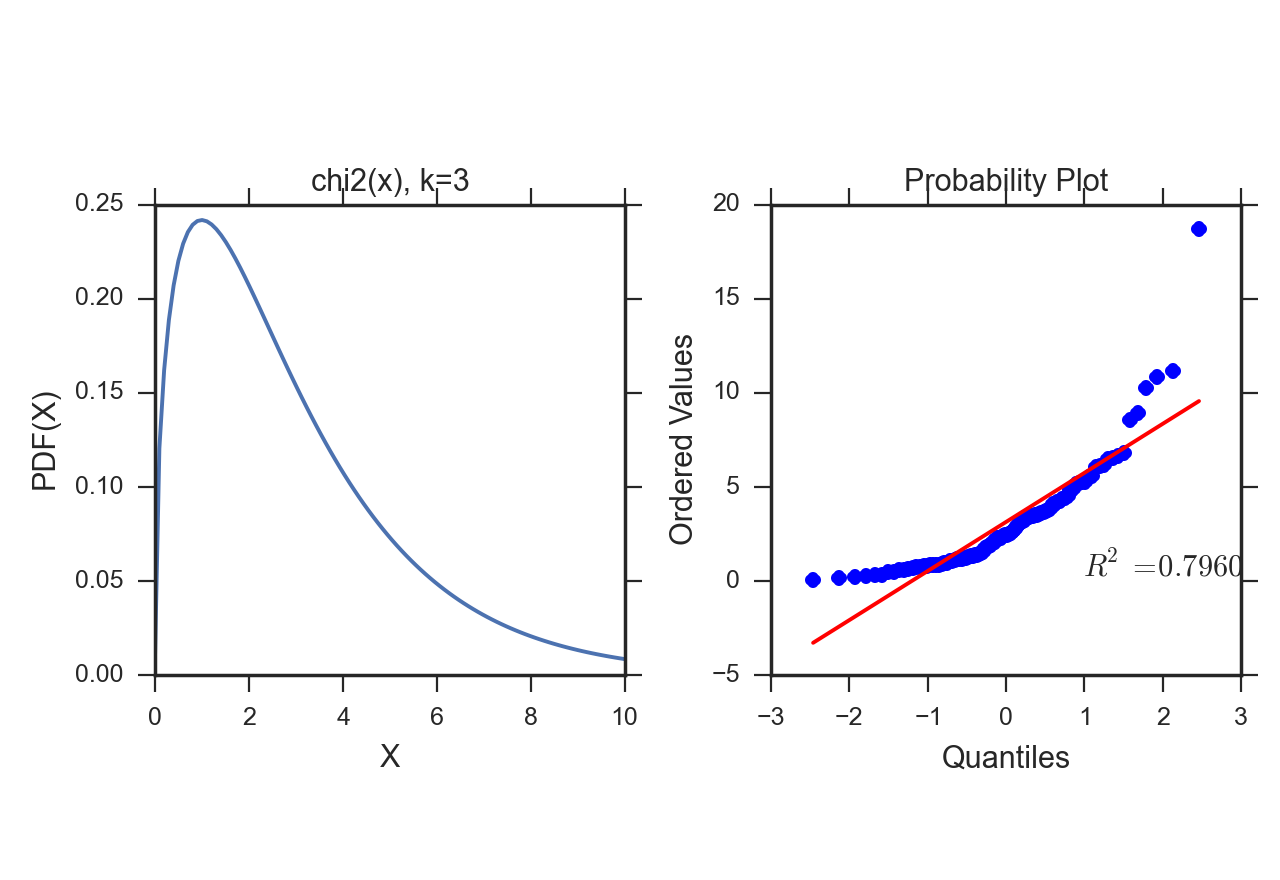
\includegraphics[width=1.0\textwidth]{../Images/chi2pp.png}\\
  \caption{Left) Probability-density-function for a Chi2-distribution (k=3), which is clearly non-normal. Right) Corresponding Probability-plot}\label{fig:qqplotChi2}
\end{figure}

To understand the principle behind those plots, look at the right plot in Fig. \ref{fig:qqplotChi2}. Here we have \emph{100} random data points from a chi2-distribution, which is clearly unsymmetrical. The x-value of the first data point is (approximately) the $1/100$-quantile of a standard normal distribution (\lstinline{stats.norm().ppf(0.01)}), which corresponds to \emph{-2.33} (The exact value is slightly shifted, because of a small correction, called "Filliben's estimate"\index{general}{Filliben's estimate}). The y-value is the smallest value of our data-set. Similarly, the second x-value corresponds approximately to \lstinline{stats.norm().ppf(0.01)}, and the second y-value is the second-lowest value of the data set, etc.

\subsubsection{Hypothesis Tests for Normality}

In tests for normality, different challenges can arise: sometimes only few samples may be available, while other times one may have many data, but some extremely outlying values. To cope with the different situations different tests for normality have been developed. These tests to evaluate normality (or similarity to some specific distribution) can be broadly divided into two categories:

\begin{enumerate}
  \item Tests based on comparison (“best fit”) with a given distribution, often specified in terms of its CDF. Examples are the Kolmogorov-Smirnov test, the Lilliefors test, the Anderson-Darling test, the Cramér-von Mises criterion, as well as the Shapiro-Wilk and Shapiro-Francia tests.
  \item Tests based on descriptive statistics of the sample. Examples are the skewness test, the kurtosis test, the D’Agostino-Pearson omnibus test, or the Jarque-Bera test.
\end{enumerate}

For example, the Lilliefors test\index{general}{test!Lilliefors}, which is based on the Kolmogorov--Smirnov test \index{general}{test!Kolmogorov-Smirnov}, quantifies a distance between the empirical distribution function of the sample and the cumulative distribution function of the reference distribution, or between the empirical distribution functions of two samples. (The original Kolmogorov-Smirnov test should not be used if the number of samples is ca. $\leq 300$.)

The Shapiro-Wilk W test\index{general}{test!Shapiro-Wilk}, which depends on the covariance matrix between the order statistics of the observations, can also be used with $\leq 50$ samples, and has been recommended by \cite{altman99} and by \cite{Ghasemi2012c}.

The \emph{Python} command \lstinline{stats.normaltest(x)} uses the D’Agostino-Pearson \emph{omnibus test}\index{general}{test!omnibus}. This test combines a skewness and kurtosis test to produce a single, global, "omnibus" statistic.

\vspace{5 mm}

\PyImg "checkNormality.py" (p \pageref{py:checkNormality}) shows how to check graphically and quantitatively if a given distribution is normal.
\index{python}{checkNormality}

\begin{figure}
  \centering
  \includegraphics[width=0.5\textwidth]{../Images/KS_Example.png}\\
  \caption{Illustration of the Kolmogorov-Smirnov statistic. Red line is CDF, blue line is an ECDF, and the black arrow is the K-S statistic (from Wikipedia).}\label{fig:ksplot}
\end{figure}


\subsection{Transformation} \index{general}{transformation}
If your data deviate significantly from a normal distribution, it is sometimes possible to make the distribution approximately normal by transforming your data. For example, data often have values that can only be positive (e.g. the size of persons), and that have  long positive tail: such data can often be made normal by applying a log transform. This is demonstrated in Figure \ref{fig:lognormal}.


\section{Hypothesis tests}\label{sec:hypotheses} \index{general}{hypotheses}

\subsection{An Example}

Assume that you are running a private educational institution. Your contract says that if your students score 110 in the final exam, where the national average is 100, you get a bonus. When the results are significantly lower, you loose your bonus (because the students are not good enough), and you have to hire more teachers; and when the results are significantly higher, you also loose your bonus (because you have spent too much money on teachers), and you have to cut back on the number of teachers.

The final exam of your 10 students produce the following scores (Fig. \ref{fig:ExampleTtest}):

\begin{lstlisting}[language=Python]
  scores = array([ 109.4, 76.2, 128.7, 93.7, 85.6, 117.7, 117.2, 87.3, 100.3, 55.1])
\end{lstlisting}

\begin{figure}[ht]
  \centering
  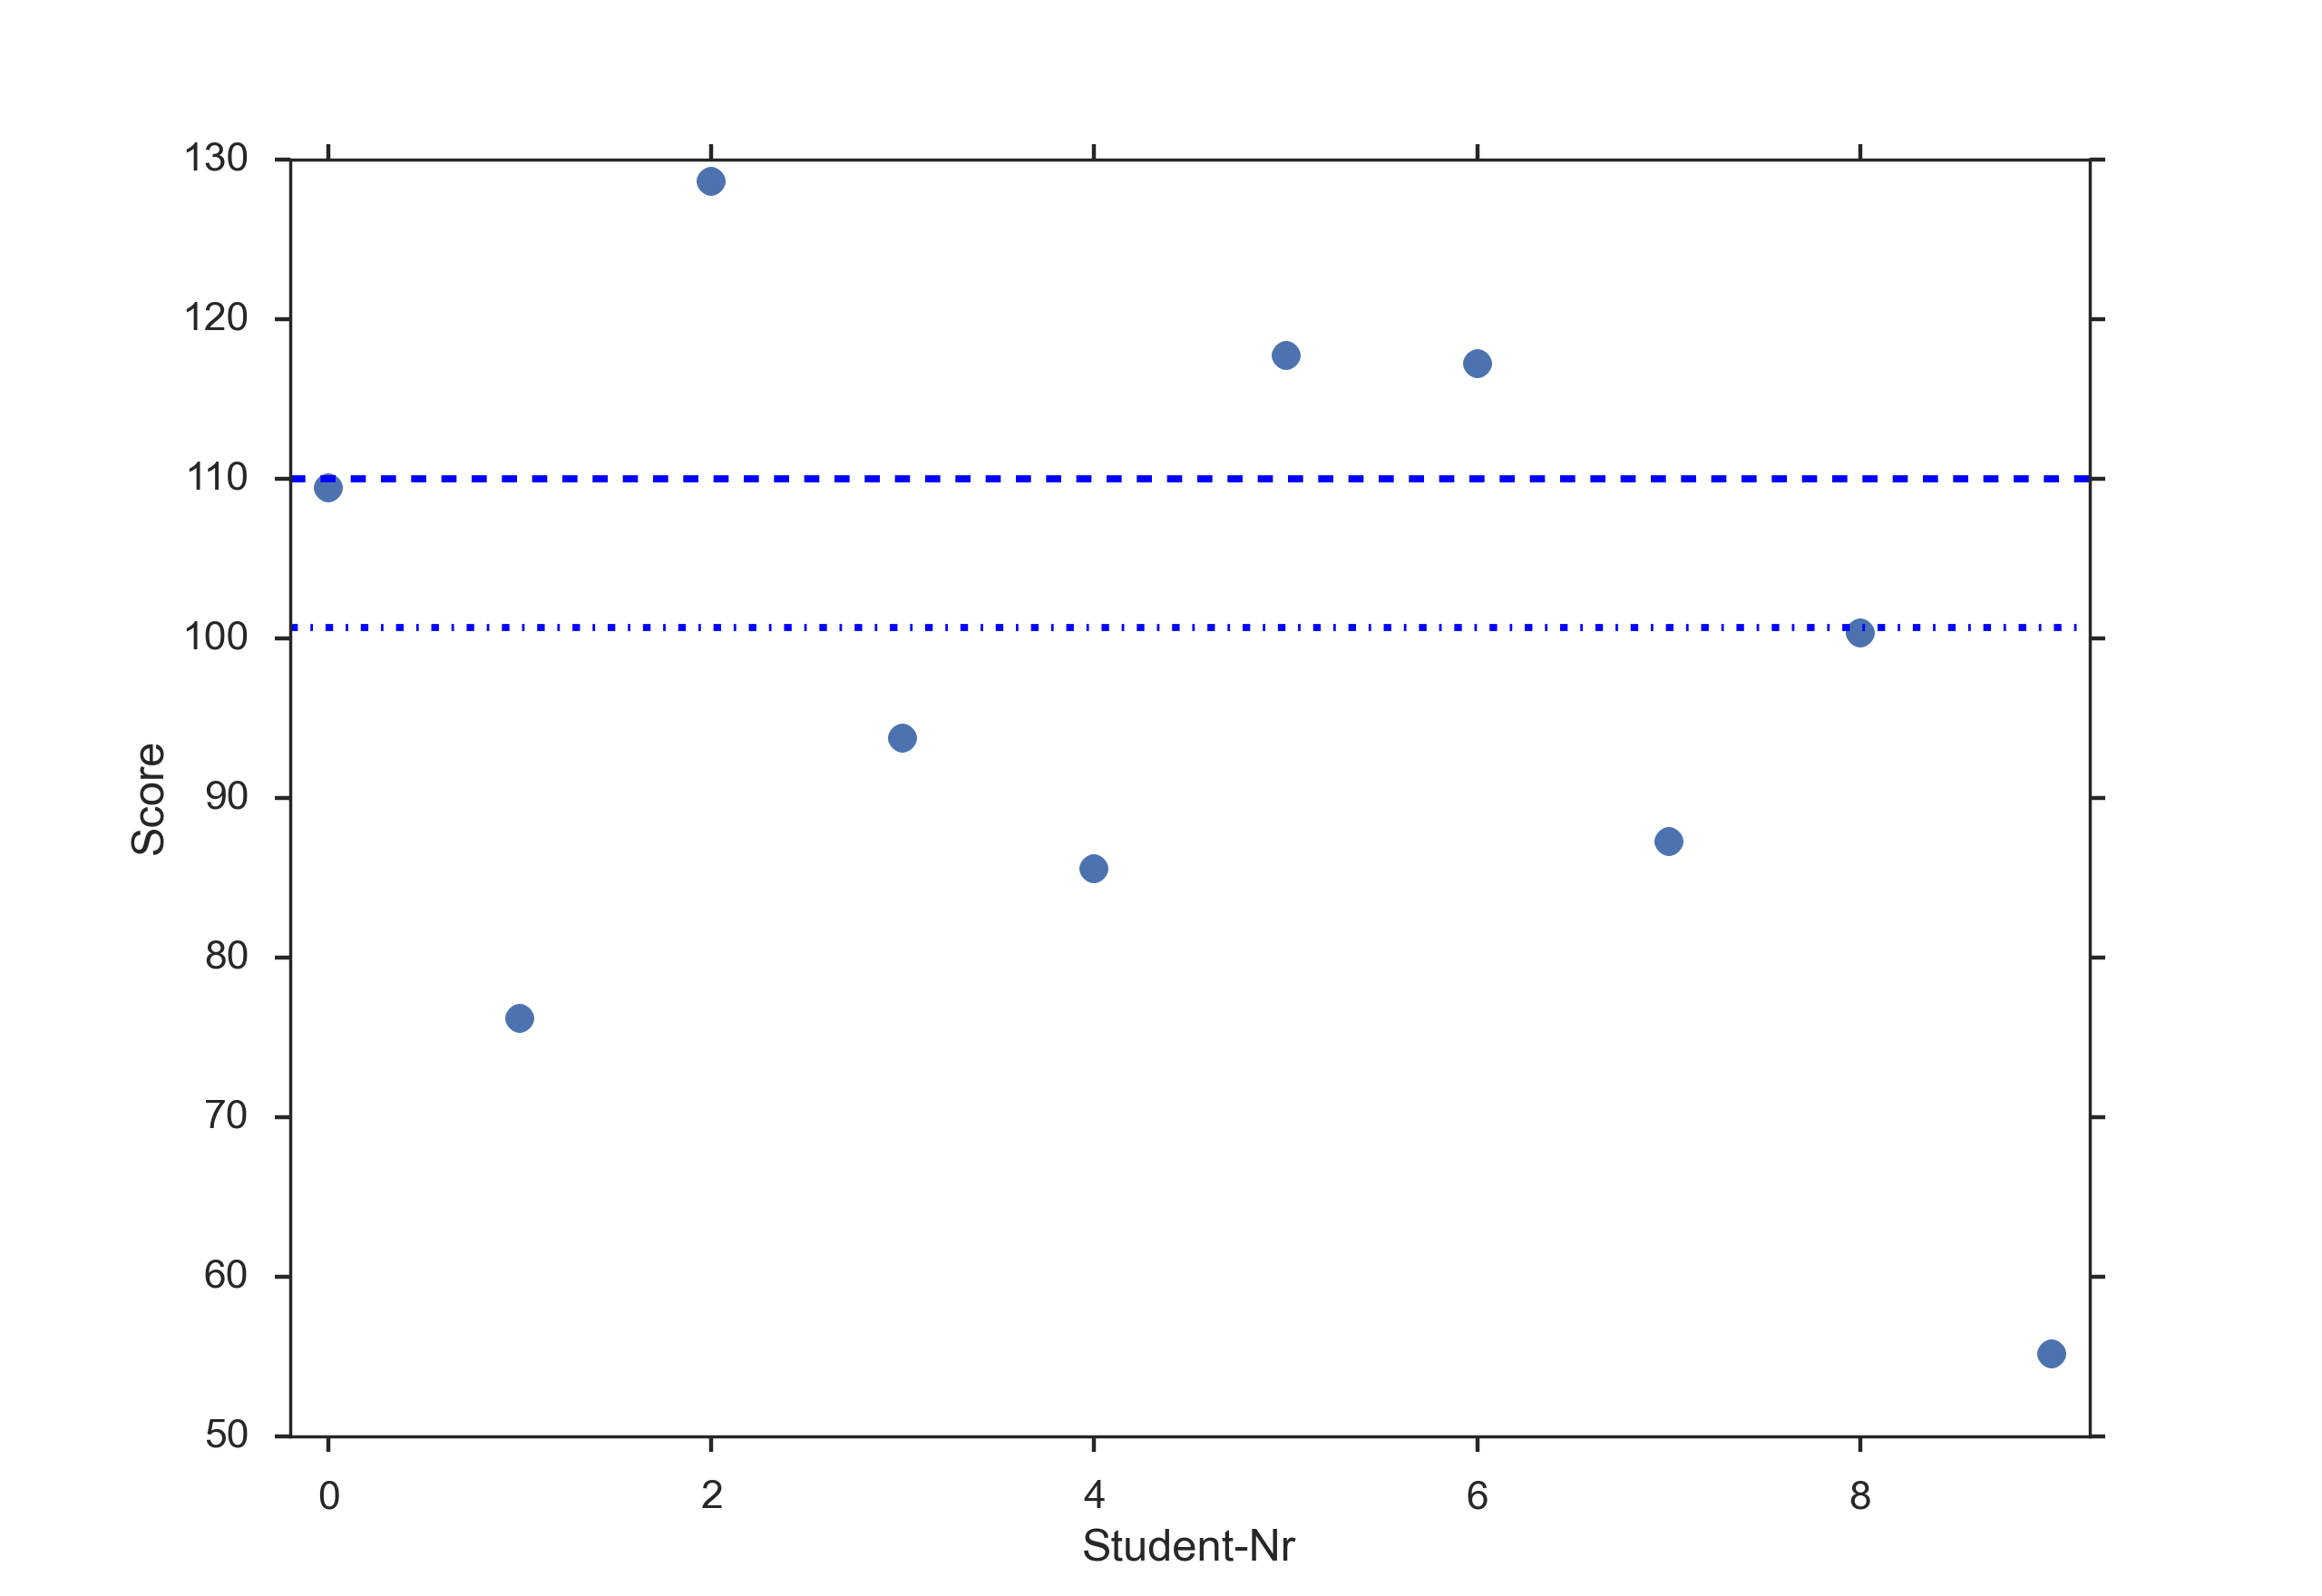
\includegraphics[width=0.75\textwidth]{../Images/fig_ExampleTtest.png}\\
  \caption{The question we ask: based on our sample mean (dashed-dotted line) and the observed variance of the data (the sample variance), do we believe that the population mean is different from 110 (dashed line)? Or in other words: our Null-hypothesis is that the difference between the population mean and 110 is zero. Can we keep our Null-hypothesis, or do we have to reject it based on the data?}\label{fig:ExampleTtest}
\end{figure}

The question we want to answer: Is the mean value of the scores (\emph{97.1}) significantly different from 110?

A \emph{normality test} (\lstinline{stats.normaltest(scores)}) indicates that the data are probably taken from a normal distribution.  Since we don't know the population variance of the results of students tested, we have to take our best guess, the sample variance (see also Fig. \ref{fig:population}). And we know that the normalized difference between sample and the population mean, the t-statistic, follows the t-distribution (Eq. \ref{eq:Tdistribution}).

The difference between our sample mean and the value we want to compare it to (\lstinline{ np.mean(scores) - 110} ) is \emph{12.9}. Normalized by the sample standard error (Eq. \ref{eq:Tdistribution}), this gives a value of \emph{t=-1.84}. Since the t-distribution is a known curve that depends only on the number of samples, and we can calculate the likelihood that we obtain a t-statistic of $|t| > 1.84$:

\begin{lstlisting}[language=Python]
    tval = (110-np.mean(scores))/stats.sem(scores)  # 1.84
    td = stats.t(len(scores)-1)                     # "frozen" t-distribution
    p = 2*td.sf(tval)                               # 0.0995
\end{lstlisting}

(The factor \emph{2} in the last line of the code is required, since we have to combine the probability of $t<-1.84$ and $t>1.84$.) Expressed in words, given our sample data, we can state that the likelihood that the population mean is \emph{110} is 9.95\%. But since a \emph{statistical difference} is only given by convention if the likelihood is less than 5\%, we conclude that the observed value of 97.1 is not significantly different from 110, and the bonus has to be paid out.

\subsection{Generalization}

Based on the previous example, the general procedure for hypothesis tests can be described as follows (the sketch in Fig. \ref{fig:population} indicates the meaning of many upcoming terms):

\begin{itemize}
  \item A random sample is drawn from a population. (In our example, the random sample is our \emph{scores}).
  \item A Null hypothesis\index{general}{null hypothesis} is formulated. ("There is Null difference between the population mean and the value of 110.")
  \item A test-statistic is calculated, from which we know the probability distribution. (Here the sample mean, since we know that the mean value of samples from a normal distribution follows the t-distribution.)
  \item Comparing the observed value of the statistic (here the obtained t-value) with the corresponding distribution (the t-distribution), we can find the likelihood that a value as extreme as or more extreme than s the observed one is found by chance. This is the so-called "p-value".
  \item If the p-value is $p<0.05$, we reject the Null-hypothesis, and speak of a "statistically significant difference". If a value of $p<0.001$ is obtained, the result is typically called "highly significant". The critical region of a hypothesis test is the set of all outcomes which cause the null hypothesis to be rejected in favor of the alternative hypothesis\index{general}{alternative hypothesis}.
\end{itemize}

In other words, the p-value states how likely it is to obtain a value as extreme or more extreme by chance alone, \emph{if the Null hypothesis is true}.

The value against which the p-value is compared is the "significance level"\index{general}{significance level}, and is often indicated with the letter $\alpha$. The significance level is a user choice, and typically set to $0.05$.

This way of proceeding to test a hypothesis is called Statistical Inference\index{general}{statistical inference}.

Remember, p only indicates the likelihood of obtaining a certain value for the test statistic if the null hypothesis is true - nothing else!

And keep in mind that improbable events do happen, even if not very frequently. For example, back in 1980 a woman named Maureen Wilcox bought tickets for both the Rhode Island lottery and the Massachusetts lottery. And she got the correct numbers for both lotteries. Unfortunately for her, she picked all the correct numbers for Massachusetts on her Rhode Island ticket, and all the  right numbers for Rhode island on her Massachusetts ticket :(  Seen statistically, the p-value for such an event would be extremely small - but it did happen anyway.

\subsubsection{Additional Examples}

\textbf{Example 1: } Let us compare the weight of two groups of subject. The Null hypothesis is that there is null difference in the weight between the two groups. If a statistical comparison of the weight produces a p-value of 0.03, this means that the probability that the null hypothesis is correct is 0.03, or 3\%. Since this probability is quite low, we say that "there is a significant difference between the weight of the two groups".

\textbf{Example 2: } If we want to check the assumption that the mean value of a group is 7, then the null hypothesis would be: "We assume that there is null difference between the mean value in our population and the value 7."

\subsection{The interpretation of the p-value, and the "p-value fallacy"}

\fbox{
\begin{minipage}{15 cm}
    \textbf{Note:} A value of $p<0.05$ for the null hypothesis has to be interpreted as follows: \emph{If the null hypothesis is true, the chance that we find a test statistic as extreme or more extreme than the one observed is less than 5\%.} This is \emph{not} the same as saying that the null hypothesis is false, and even less so, that an alternative hypothesis is true!
\end{minipage}
}

\vspace{5 mm}

Stating a p-value alone is no longer state-of-the-art for the statistical analysis of data. You should also state the confidence intervals for the parameter that you investigate.

Therefore research is sometimes divided into "exploratory research"\index{general}{exploratory research} and "confirmatory research"\index{general}{confirmatory research}. Take for example the case of Matt Motyl, a Psychology PhD student at the University of Virginia. In 2010, data from his study of nearly 2000 people indicated that political moderates saw shades of grey more accurately than people with more extreme political opinions, with a p-value of 0.01. However, when he tried to reproduce the data, the p-value dropped down to 0.59. So while the \emph{exploratory research} showed that a certain hypothesis may be likely, the \emph{confirmatory research} showed that the hypothesis did not hold (\cite{Nuzzo2014}).

\cite{sellke2001} have investigated this question in detail, and recommend to use a "calibrated p-value" to estimate the probability of making a mistake when rejecting the null hypothesis, when the data produce a p-value $p$:

\begin{equation}\label{eq:pFallacy}
    \alpha(p)= \frac{1}{1 + \frac{1}{-e \; p \; log(p)}}
\end{equation}

with $e=exp(1)$, and $log$ the natural logarithm. For example, $p=0.05$ leads to $\alpha=0.29$, and $p=0.01$ to $\alpha=0.11$.

\subsection{Types of Error}
In hypothesis testing, two types of errors can occur:

\subsubsection{Type I errors} \index{general}{error!Type I} \index{general}{power}
\gls{TypeI} are errors, where you get a significant result despite the fact that the hypothesis is true. The likelihood of a Type I error is commonly indicated with $\alpha$, and is set before you start the data analysis. In quality control, a Type I error is called Producer Risk, because you keep a produced item despite the fact that it meets the regulatory requirements.

For example, assume that the population of young Austrian adults has a mean IQ of 105 (i.e. we are smarter than the rest) and a standard deviation of 15. We now want to check if the average FH student in Linz has the same IQ as the average Austrian, and we select 20 students. We set $\alpha=0.05$, i.e. we set our significance level to 95\%.
Let us now assume that the average student has in fact the same IQ as the average Austrian. If we repeat our study 20 times, we will find one of those 20 times that our sample mean is significantly different from the Austrian average IQ. Such a finding would be a false result, despite the fact that our assumption is correct, and would constitute a type I error.

\subsubsection{Type II errors and Test Power}\index{general}{error!Type II}
If we want to answer the question "How much chance do we have to reject the null hypothesis when the alternative is in fact true?" Or in other words, "What’s the probability of detecting a real effect?" we are faced with a different problem. To answer these questions, we need an "alternative hypothesis".

For the example given above, an alternative hypothesis could be: "We assume that our population has a mean value of 6."

A \gls{TypeII} is an error, where you do \emph{not} get a significant result, despite the fact that the null-hypothesis is false.  In quality control, a Type II error is called a Consumer Risk, because the consumer obtains an item that does not meet the regulatory requirements.

The probability for this type of error is commonly indicated with $\beta$. The "power" of a statistical test is defined as $(1-\beta)*100$, and is the chance of correctly accepting the alternate hypothesis. Figure \ref{fig:power1} shows the meaning of the power of a statistical test. Note that for finding the power of a test, you need an alternative hypothesis.

\subsubsection{Type II Errors and P-value}

In other words, p values are often used to measure evidence against a hypothesis. Unfortunately, they are often incorrectly viewed as an error probability for rejection of the hypothesis, or, even worse, as the posterior probability (i.e. after the data have been collected) that the hypothesis is true. As an example, take the case where the alternative hypothesis is that the mean is just a fraction of one standard deviation larger than the mean under the null hypothesis: in that case, a sample that produces a p-value of 0.05 may just as likely be produced if the alternative hypothesis is true as if the null hypothesis is true!

\subsection{Sample Size}\index{general}{sample size}
The power of a statistical test depends on four factors:

\begin{enumerate}
  \item  $\alpha$, the probability for Type I errors
  \item  $\beta$, the probability for Type II errors ( $\Rightarrow$ power of the test)
  \item  $d$, the effect size, i.e. the magnitude of the investigated effect relative to $\sigma$, the standard deviation of the sample
  \item  $n$, the sample size
\end{enumerate}

Only 3 of these 4 parameters can be chosen, the $4^{th}$ is then automatically fixed.

The absolute size of the difference $D$ between mean treatment outcomes that will answer the clinical question being posed is often called Clinical Significance or Clinical Relevance.

\begin{figure}[!ht]
  \centering
  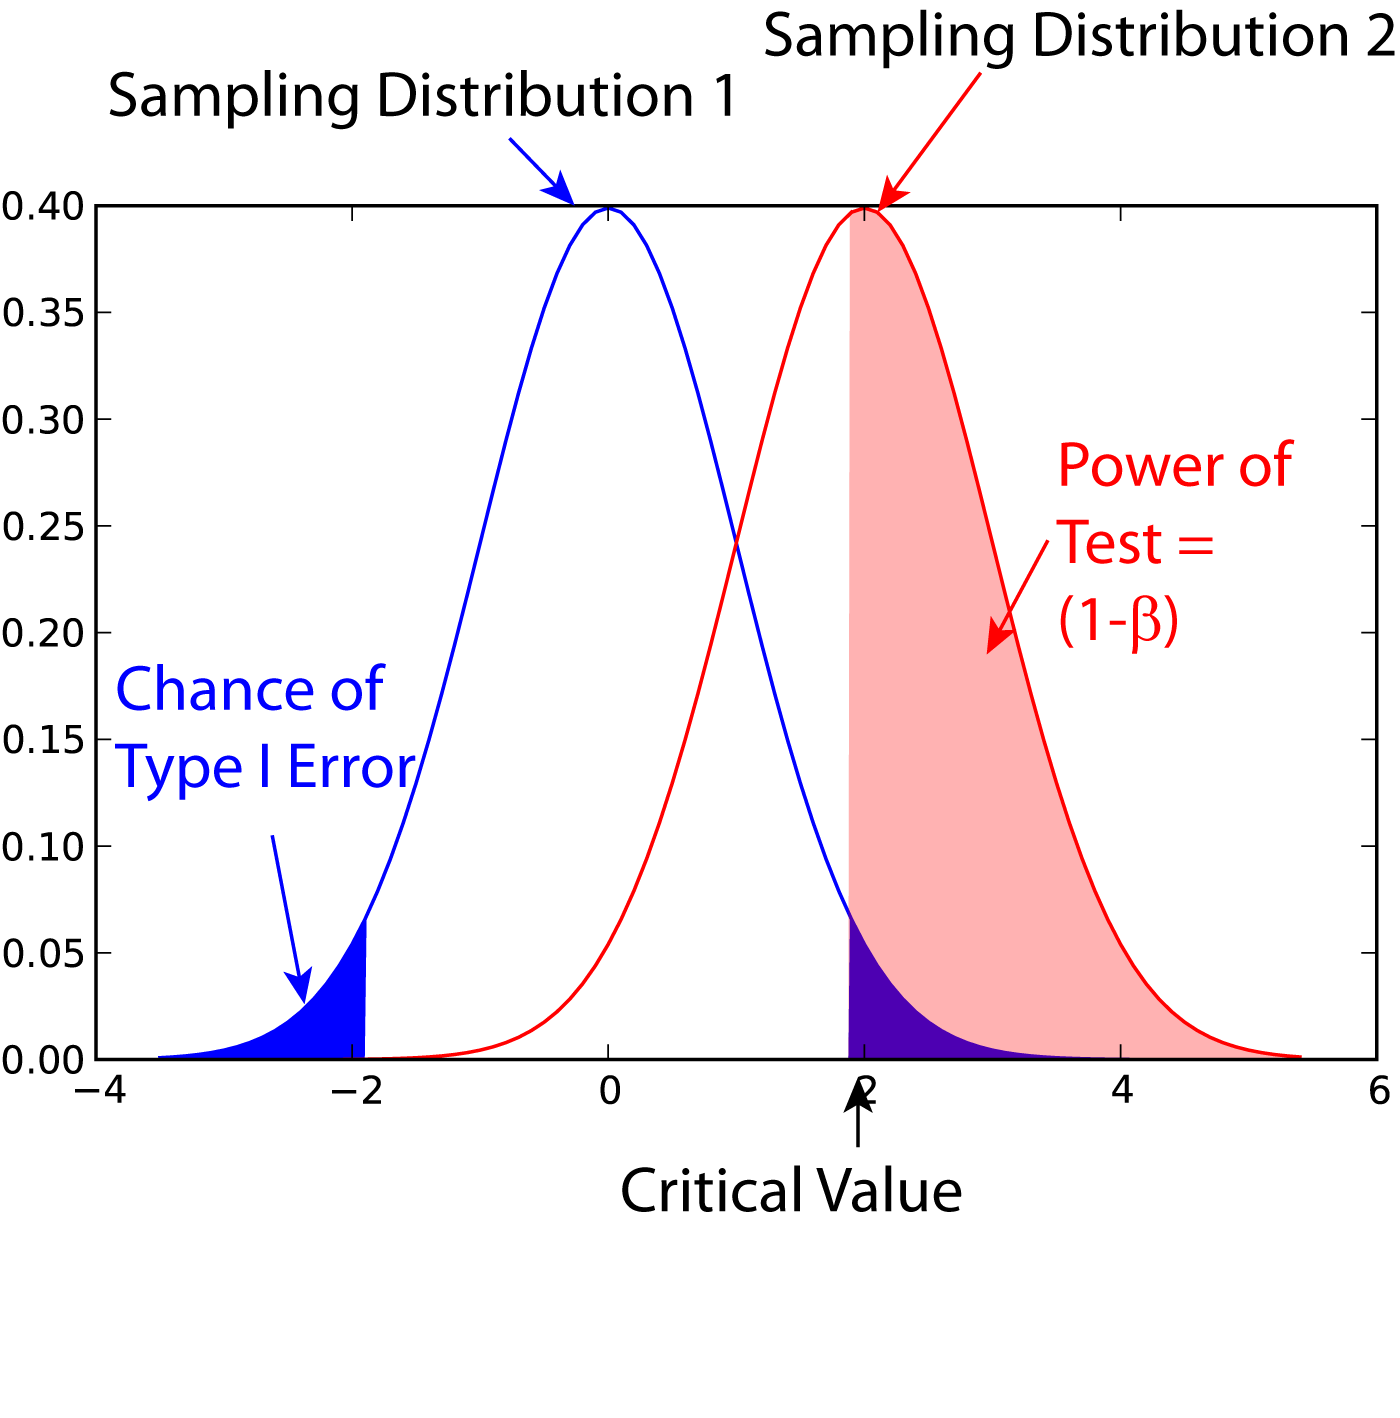
\includegraphics[width=0.5\textwidth]{../Images/power1.png}\\
  \caption{\emph{Power} of a statistical test, for comparing the mean value of two sampling distributions.}\label{fig:power1}
\end{figure}

\begin{figure}[!ht]
  \centering
  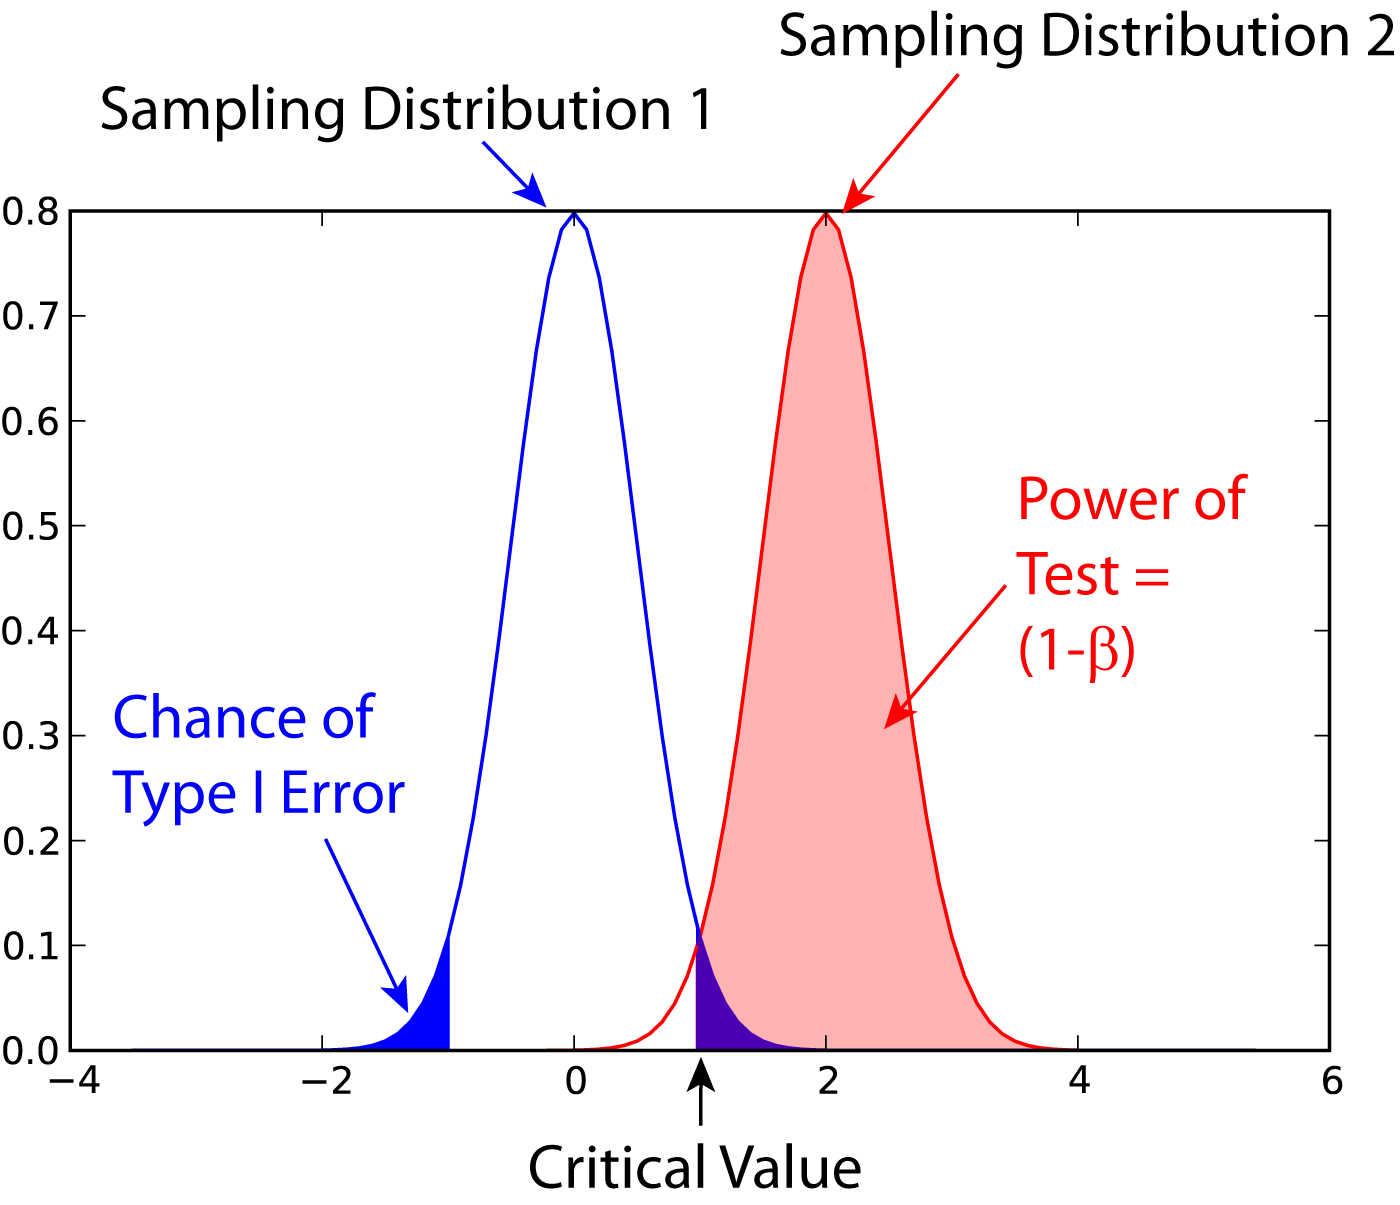
\includegraphics[width=0.5\textwidth]{../Images/power2.png}\\
  \caption{Effect of an increase in sampling size on the power of a test.}\label{fig:power2}
\end{figure}

\subsubsection{Examples for some special cases}

\paragraph{Test on One Mean}
If we have the hypothesis that the data population has a mean value of $x_1$ and a standard deviation of $\sigma$, and the actual population has a mean value of $x_1+D$ and the same standard deviation, we can find such a difference with a minimum sample number of

\begin{equation}
  n = \frac{{({z_{1 - \alpha /2}} + {z_{1 - \beta }})}^2}{d^2}
\end{equation}

Here $z$ is the standardized normal variable (see also chapter \ref{sec:normalDistribution})

\begin{equation}
  z = \frac{x-\mu}{\sigma} .
\end{equation}

and $d = \frac{D}{\sigma}$ the effect size.

In words, if the real mean has a value of $x_1$, we want to detect this correctly in at least $1-\alpha\%$ of all tests; and if the real mean is shifted by $D$ or more, we want to detect this with a likelihood of at least $1-\beta\%$.

\paragraph{Test Between Two Different Populations}
For finding a difference between two normally distributed means, with standard deviations of $\sigma_1$ and $\sigma_2$, the minimum number of samples we need in each group to detect an absolute difference $D$ is

\begin{equation}
  {n_1} = {n_2} = \frac{{({z_{1 - \alpha /2}} + {z_{1 - \beta }})}^2(\sigma _1^2 + \sigma _2^2)}{D^2} .
\end{equation}

\subsubsection{Python Solution}

\emph{statsmodels} makes clever use of the fact that 3 of the 4 factors mentioned above are independent, and combines it with the \emph{Python} feature of "named parameters" to provide a program that takes 3 of those parameters as input, and calculates the remaining $4^{th}$ parameter. For example,

\begin{lstlisting}[language=Python]
    In [1]: from statsmodels.stats import power

    In [2]: nobs = power.tt_ind_solve_power(effect_size = 0.5, alpha =0.05, power=0.8)
    In [3]: print(nobs)
    Out[3]: 63.76561177540974
\end{lstlisting}

tells us that if we compare two groups with the same number of subjects and the same standard deviation, require an $\alpha=0.05$ a test power of $80\%$, and we want to detect a difference between the groups that is half the standard deviation, we need to test 64 subjects.

Similarly,

\begin{lstlisting}[language=Python]
    In [4]: effect_size = power.tt_ind_solve_power(alpha =0.05, power=0.8, nobs1=25)
    In [5]: print(effect_size)
    Out[5]: 0.8087077886680407
\end{lstlisting}

tells us that if we have an $\alpha=0.05$, a test power of $80\%$, and 25 subjects in each group, then the smallest difference between the groups is 81\% of the sample standard deviation.

The corresponding command for one sample t-tests is \lstinline{tt_solve_power}.

\subsubsection{Programs: SampleSize}

\PyImg "sampleSize.py" (p \pageref{py:sampleSize}): sample size calculation for normally distributed groups with arbitrary standard deviations.
\index{python}{sampleSize}


\section{Sensitivity and Specificity}

Some of the more confusing terms in statistical analysis are \gls{sensitivity} \index{general}{sensitivity} and \gls{specificity} \index{general}{specificity}. A related topic are the "positive predictive value (PPV)" \index{general}{positive predictive value} and the "negative predictive value (NPV)" \index{general}{negative predictive value}. The following diagram shows how the four are related:

\begin{figure}[ht]
  \centering
  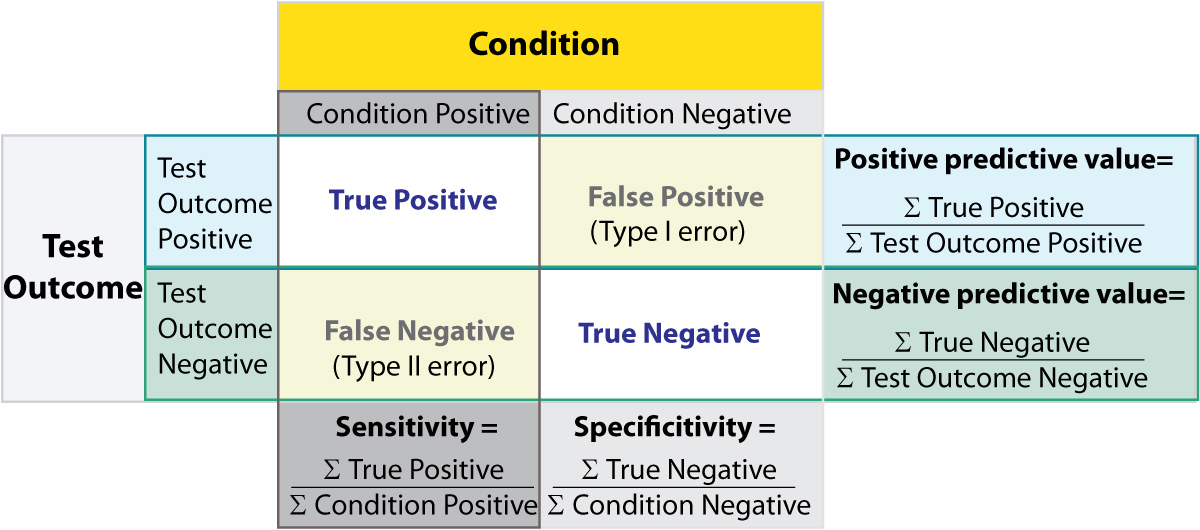
\includegraphics[width=0.9\textwidth]{../Images/Sensitivity_Specificity_Diagram.jpg}\\
  \caption{Relationship between sensitivity, specificity, positive predictive value and negative predictive value.}\label{fig:sens_spec_diagram}
\end{figure}

\begin{description}
  \item[Sensitivity] Also called \gls{power}. Proportion of positives that are correctly identified by a test = probability of a positive test, given the patient is ill.
  \item[Specificity] Proportion of negatives that are correctly identified by a test = probability of a negative test, given that patient is well.
  \item[Positive Predictive Value (PPV)] Proportion of patients with positive test results who are correctly diagnosed.
  \item[Negative Predictive Value (NPV)] Proportion of patients with negative test results who are correctly diagnosed.
\end{description}

For example, pregnancy tests have a high sensitivity: when a woman is pregnant, the probability that the test is positive is very high.

In contrast, an indicator for an attack with atomic weapons on the White House should have a very high specificity: if there is no attack, the probability that the test goes on should be very, very small.

Sensitivity and specificity characterize a test, while PPV and NPV are the parameters that tell the doctor how to interpret a test result.

While sensitivity and specificity characterise a test and are independent of prevalence, they do not indicate what portion of patients with abnormal test results are truly abnormal. This information is provided by the positive/negative predictive value. However, as Fig. \ref{fig:prevalence} indicates, these values are affected by the prevalence \index{general}{prevalence} of the disease. The "prevalence" of a disease indicates how many out of 100'000 people are affected by it; in contrast, the "incidence" gives the number of newly diagnosed cases per 100'000 people. In summary, we need to know the prevalence of the disease as well as the PPV/NPV of a test to provide a sensible interpretation of the test results.

\begin{figure}[ht]
  \centering
  \includegraphics[width=0.75\textwidth]{../Images/Sensitivity_Specificity.png}\\
  \caption{Effect of prevalence on PPV and NPV. "T" stands for "test", and "P" for "patient". (For comparison with below: T+P+ = TP, T-P- = TN, T+P- = FP, and T-P+ = FN)} \label{fig:prevalence}
\end{figure}

Figure \ref{fig:sens_spec_example} gives a worked example:

\begin{figure}[ht]
  \centering
  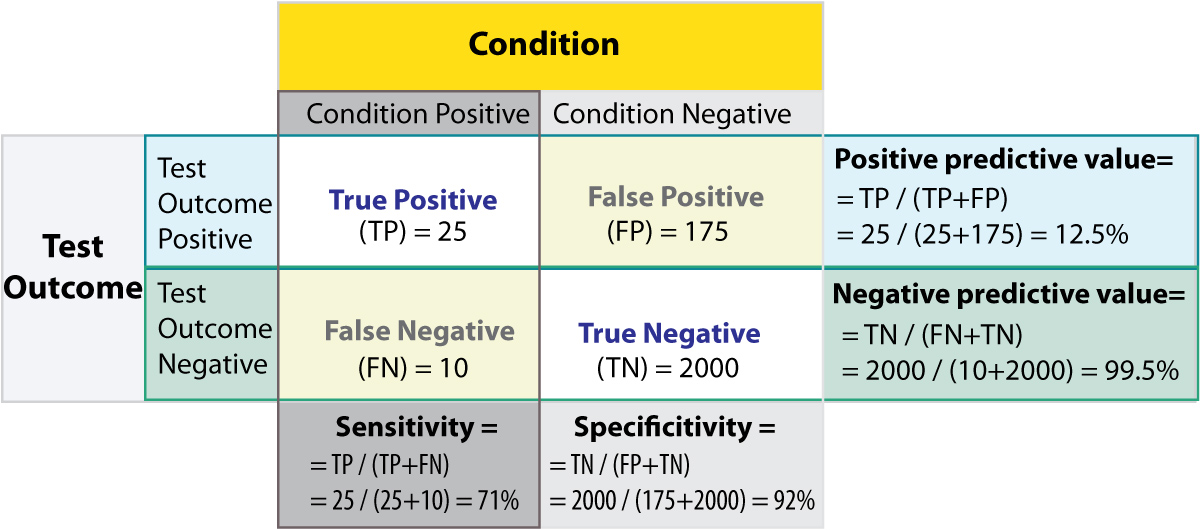
\includegraphics[width=0.9\textwidth]{../Images/Sensitivity_Specificity_Example.jpg}\\
  \caption{Worked example.}\label{fig:sens_spec_example}
\end{figure}

\paragraph{Related calculations}

\begin{itemize}
  \item False positive rate ($\alpha$) = type I error = $1 - specificity$ = $\frac{FP}{FP + TN}$ = $\frac{180}{180+1820}$ = 9\%
  \item False negative rate ($\beta$) = type II error = $1 - sensitivity$ = $\frac{FN}{TP + FN}$ = $\frac{10}{20+10}$ = 33\%
  \item Power = sensitivity = $1 - \beta$
  \item Likelihood ratio positive = $\frac{sensitivity}{1−specificity}$ = $\frac{66.67\%}{1−91\%}$ = 7.4
  \item Likelihood ratio negative = $\frac{1−sensitivity}{specificity}$ = $\frac{1−66.67\%}{91\%}$ = 0.37
\end{itemize}

Hence with large numbers of false positives and few false negatives, a positive test outcome in this example is in itself poor at confirming cancer (PPV = 12.5\%) and further investigations must be undertaken; it did, however, correctly identify 71\% of all cancers (the sensitivity). However as a screening test, a negative result is very good at reassuring that a patient does not have cancer (NPV = 99.5\%) and at this initial screen correctly identifies 92\% of those who do not have cancer (the specificity).

\section{ROC Curve}\index{general}{ROC curve}

Closely related to sensitivity and specificity is the \acrfull{roc} (ROC) curve. This is a graph displaying the relationship between the true positive rate (on the vertical axis) and the false positive rate (on the horizontal axis). The technique comes from the field of engineering, where it was developed to find the predictor which best discriminates between two given distributions. In the ROC-curve (Figure \ref{fig:ROC}) this point is given by the value with the largest distance to the diagonal.

\begin{figure}[ht]
  \centering
  \includegraphics[width=0.75\textwidth]{../Images/ROC.png}\\
  \caption{Top: Probability density functions for two distributions. Bottom: corresponding \emph{ROC-curve}.}\label{fig:ROC}
\end{figure}

\section{Common Statistical Tests for Comparing Groups}

Table \ref{table:tests} gives an overview of the most common statistical tests for different combinations of data.
\begin{table}
  \centering
  \footnotesize{
  \begin{tabular}{ | p{5cm} || p{5cm} | p{5cm} | }
     \hline
     No. of Groups Compared  & \textbf{Independent Samples} & \textbf{Paired Samples} \\ \hline
     \textbf{Groups of Nominal Data} & & \\ \hline
     2 or more & Fisher's exact test or Chi-Square test & McNemar's test \\ \hline
     \textbf{Groups of Ordinal Data} & & \\ \hline
     2 & Mann-Whitney U test & Wilcoxon signed rank test \\ \hline
     3 or more & Kruskal-Wallis test & Friedman test \\ \hline
     \textbf{Groups of Continuous Data} & & \\ \hline
     2 & Student's t-test or Mann-Whitney test & Paired t-test or Wilcoxon signed-rank test \\ \hline
     3 or more & ANOVA or Kruskal-Wallis test & Repeated Measures ANOVA or Friedman test \\ \hline

  \end{tabular}
  }

  \caption{Typical tests for statistical problems.}\label{table:tests}
\end{table}

\subsection{Examples}

\begin{description}
  \item[2 groups, nominal] male/female, blond-hair/black-hair. E.g. "Are females more blond than males?"
  \item[2 groups, nominal, paired] 2 labs, analysis of blood samples. E.g. "Does the blood analysis from Lab1 indicate more infections than the analysis from Lab2?"
  \item[2 groups, ordinal] black/white, ranking 100m sprint. E.g. "Are black sprinters more successful than white sprinters?"
  \item[2 groups, ordinal, paired] sprinters, before/after diet. E.g. "Does a chocolate diet make sprinters more successful?"
  \item[3 groups, ordinal] black/white/chinese, ranking 100m sprint. E.g. "Does ethnicity have an effect on the success of sprinters?"
  \item[3 groups, ordinal, paired] sprinters, before/after diet. E.g. "Does a rice diet make Chinese sprinters more successful?"
  \item[2 groups, continuous] male/female, IQ. E.g. "Are women more intelligent than men?"
  \item[2 groups, continuous, paired] male/female, looking at diamonds. E.g. "Does looking at diamonds raise the female heart-beat more than the male?
  \item[3 groups, continuous] Tyrolians, Viennese, Styrians; IQ. E.g. "Are Tyrolians smarter than people from other Austrian federal states?"
  \item[3 groups, continuous, paired] Tyrolians, Viennese, Styrians; looking at mountains. E.g. "Does looking at mountains raise the heartbeat of Tyrolians more than those of other people?"
\end{description}

\section{Exercises}
\begin{enumerate}
  \item
  \begin{enumerate}
    \item Read in the data from 'Data\textbackslash amstat\textbackslash calcium.dat.txt'.
    \item Check for erroneous entries.
    \item Check the Alkaline Phosphatase levels for normality. Use a log-transform on the data, and re-check.
  \end{enumerate}

\end{enumerate}


\chapter{Test of Means of Continuous Data}

\section{Distribution of a Sample Mean}

\subsection{One sample t-test for a mean value} \index{general}{test! t-test, one sample}

To check the mean value of normally distributed data against a reference value, we typically use the \emph{one sample t-test}, which is based on the \emph{t-distribution}.

If we knew the mean and the standard deviation of a normally distributed population, we could calculate the corresponding standard error, and use values from the normal distribution to determine how likely it is to find a certain mean value, given the population mean and standard deviation. However, in practice we have to \emph{estimate} the mean and standard deviation from the sample, and the t-distribution for the mean slightly deviates from a normal distribution.

\subsubsection{Example}

Let us look at a specific example: we take 100 normally distributed data, with a mean of 7 and with a standard deviation of 3.
What is the chance of finding a mean value at a distance of 0.5 or more from the mean? \emph{Answer: The probability from the t-test in the example is 0.057, and from the normal distribution 0.054}

Since it is very important to understand the basic principles of how we arrive at the t-statistic and the corresponding p-value for this test, let me illustrate the underlying statistics by going step-by-step through the analysis:

\begin{figure}
  \centering
  \includegraphics[width=0.75\textwidth]{../Images/ttestExplained.png}\\
  \caption{Left: Frequency histogram of the sample data, together with a normal fit. The sample mean, which is very close to the population mean, is indicated with a yellow triangle; the value to be checked with a red triangle. Right: sampling distribution of t (for n-1 degrees of freedom). At the bottom the normalized value of sample mean (yellow triangle) and value to be checked (red triangle). The red shaded area corresponds to the p-value.}\label{fig:ttestExplained}
\end{figure}

\begin{itemize}
  \item We have a population, with a mean value of 7 and a standard deviation of 3.
  \item From that population an observer takes 100 random samples. The sample mean is 7.10, close to but different from the real mean. The sample standard deviation is 3.12, and the standard error of the mean 0.312. This gives the observer an idea about the variability of the population.
  \item The observer knows that the distribution of the real mean follows a t-distribution, and that the \emph{standard error of the mean} characterizes the width of that distribution.
  \item How likely it is that the real mean has a value of $x_0$ (e.g. 6.5, indicated by the red triangle in Fig. \ref{fig:ttestExplained}, left)? To find that out, this value has to be transformed, by subtracting the sample mean, and dividing by the standard error. (Fig. \ref{fig:ttestExplained}, right). This provides the \emph{t-statistic} for this test (-1.93).
  \item The corresponding \emph{p-value}, which tells us how likely it is that the real mean has a value of 6.5 or more extreme relative to the sample mean, is given by the red shaded area under the curve-wings: \emph{2*CDF(t-statistic) = 0.057}, which means that the difference to 6.5 is just not significant. (The factor "2" comes from the fact that we have to check in both tails.)
\end{itemize}

\PyImg "oneSample.py" (p \pageref{py:oneSample}): Sample analysis for one group of continuous data.
\index{python}{oneSample}

%To illustrate the ideas behind the use of distribution functions, let us go step-by-step through the analysis of the following problem:
%Being 50 years old, 175 cm tall, and moderately active, my daily nutritional requirement is 2460 cal/day. On 10 subsequent days, I have carefully listed my food intake, and obtained the following numbers of calories for each day: [2784, 2632, 2771, 2495, 2435, 2513, 2633, 2737, 2687, 2647]. My question now: is this too much - do I have to cut back on my chocolate??
%
%\begin{itemize}
%  \item Find the mean and standard deviation of the best-fit normal distribution (mean = 2633.4, std = 113.3).
%  \item Calculate the CDF at the interesting value (2460 cal/day) (CDF(2460) = 0.06).
%  \item Interpret the result (\emph{"not significant"}).
%\end{itemize}
%
%\begin{figure}
%  \centering
%  \includegraphics[width=0.85\textwidth]{../Images/pdf_checkMean.png}\\
%  \caption{Check if the mean of the fitted curve is significantly different from the value to be checked.}\label{fig:pdf_checkValue}
%\end{figure}


\subsection{Wilcoxon signed rank sum test}\index{general}{test!Wilcoxon signed rank sum}

If our data are not normally distributed, we cannot use the t-test (although this test is fairly robust against deviations from normality, see Fig. \ref{fig:ttest_stability}). Instead, we must use a \emph{non-parametric} test on the mean value. We can do this by performing a \emph{Wilcoxon signed rank sum test}.
 \footnote{Python Example: scipy.stats.wilcoxon, in "univariate.py"},\footnote{The following description and example has been taken from \cite{altman99}, Table 9.2}
This method has three steps:

\begin{enumerate}
  \item Calculate the difference between each observation and the value of interest.
  \item Ignoring the signs of the differences, rank them in order of magnitude.
  \item Calculate the sum of the ranks of all the negative (or positive) ranks, corresponding to the observations below (or above) the chosen hypothetical value.
\end{enumerate}

In Table \ref{tab:wilcoxon} you see an example, where the significance to a deviation from the value of 7725 is tested. The rank sum of the negative values gives $3+5=8$, and can be looked up in the corresponding tables to be significant. In practice, your computer program will nowadays do this for you. This example also shows another feature of rank evaluations: tied values (here $7515$) get accorded their mean rank (here $1.5$).

\begin{table}
  \centering
  \begin{tabular}{l p{2cm} p{2cm} p{2cm}}
     \hline
     Subject & Daily energy intake (kJ) & Difference from 7725 kJ & Ranks of differences \\
     1 & 5260 & 2465 & 11 \\
     2 & 5470 & 2255 & 10 \\
     3 & 5640 & 2085 & 9 \\
     4 & 6180 & 1545 & 8 \\
     5 & 6390 & 1335 & 7 \\
     6 & 6515 & 1210 & 6 \\
     7 & 6805 & 920 & 4 \\
     8 & 7515 & 210 & 1.5 \\
     9 & 7515 & 210 & 1.5 \\
     10 & 8230 & -505 & 3 \\
     11 & 8770 & -1045 & 5 \\
     \hline
   \end{tabular}
  \caption{Daily energy intake of 11 healthy women with rank order of differences (ignoring their signs) from the recommended intake of 7725 kJ.}\label{tab:wilcoxon}
\end{table}


\section{Comparison of Two Groups} \index{general}{test! t-test, paired}

\subsection{Paired T-Test}
When we compare two groups with each other, we have to distinguish between two cases. In the first case, we compare two values recorded from the same subject at two specific times. For example, we measure the size of students when they enter primary school and after their first year, and check if they have grown. Since we are only interested in the \emph{difference} between the first and the second measurement, this test is called \gls{paired}, and is essentially equivalent to a one-sample t-test for the mean difference.

\subsection{Unpaired T-Test}
An \gls{unpaired} is if we compare two independent groups. For example, we can compare the effect of a two medications given to two different groups of patients, and compare how the two groups respond. This is called an \emph{unpaired t-test}, or \emph{t-test for two independent groups}.

If we have two independent samples the variance of the difference between their means is the \emph{sum} of the separate variances, so the standard error of the difference in means is the square root of the sum of the separate variances:

\begin{align*}
   se({{\bar x}_1} \pm {{\bar x}_2}) &= \sqrt {\operatorname{var} ({{\bar x}_1}) + \operatorname{var} ({{\bar x}_2})}  \\
   &= \sqrt {{{\left\{ {se({{\bar x}_1})} \right\}}^2} + {{\left\{ {se({{\bar x}_2})} \right\}}^2}}  \\
   &= \sqrt {\frac{{s_1^2}}{{{n_1}}} + \frac{{s_2^2}}{{{n_2}}}}  \\
\end{align*}

where $\bar{x}_i$ is the mean of the i-th sample, and \emph{se} indicates the \emph{standard error}.

Expressed in words, \emph{The variance of a sum of independent random variables equals the sum of the variances.}

\subsection{Non-parametric Comparison of Two Groups: Mann-Whitney Test} \index{general}{test!Mann-Whitney}\label{test:Mann-Whitney}

If the measurement values from the two groups are not normally distributed we have to resort to a non-parametric test. The most common test for that is the \emph{Mann-Whitney(-Wilcoxon) test}. Watch out, because this test is sometimes also referred to as \emph{Wilcoxon rank-sum test}. This is different from the \emph{Wilcoxon signed rank sum test}!

\PyImg "twoSample.py" (p \pageref{py:twoSample}): Comparison of two groups, paired and unpaired.
\index{python}{twoSample}

\subsection{Statistical Hypothesis Tests vs Statistical Modeling}

With the advent of cheap computing power, statistical modeling has been a booming field. This has also affected classical statistical analysis, as most problems can be viewed from two perspectives: you can either make a statistical hypothesis, and verify or falsify that hypothesis; or you can make a statistical model, and analyse the significance of the model parameters.

Let me use a classical t-test as an example.

\subsubsection{Classical t-test}

Let us take performance measurements from a racing team, on two different occasions. During Race\_1, the members of the team achieve a score of [ 79, 100, 93, 75, 84, 107, 66, 86, 103, 81, 83, 89, 105, 84, 86, 86, 112, 112, 100, 94], and during Race\_2 [ 92, 100, 76, 97, 72, 79, 94, 71, 84, 76, 82, 57, 67, 78, 94, 83, 85, 92, 76, 88].

These numbers can be generated, and a t-test comparing the two groups can be done, with the following Python commands:

\begin{lstlisting}
    from scipy import stats
    random.seed(123)
    race_1 = np.round(randn(20)*10+90)
    race_2 = np.round(randn(20)*10+85)
    (t, pVal) = stats.ttest_rel (race_1, race_2)
    print('The probability that the two distributions are equal is {0}'.format(pVal))
\end{lstlisting}

The command \lstinline{random.seed(123)} initializes the random number generator with the number $123$, which ensures that two consecutive runs of this code produce the same result, corresponding to the numbers given above.

\subsubsection{Statistical Modeling}

\begin{lstlisting}
    import pandas as pd
    import statsmodels.formula.api as sm
    np.random.seed(123)
    df = pd.DataFrame({'Race1': race_1, 'Race2':race_2})
    result = sm.ols(formula='I(Race2-Race1) ~ 1', data=df).fit()
    print(result.summary())
\end{lstlisting}

The important line is the last but one, which produces the $results$. Thereby the \emph{ordinary least square (ols)} function from \emph{statsmodels} tests the model which describes the difference between the results of \emph{Race1} and those of \emph{Race2} with only an \emph{offset} (also called \emph{intercept} in the language of modeling). In other words, our model has only one paramter, the \emph{intercept}. The results below show that the probability that this intercept is 0 is only 0.03: the difference is \emph{significant}.

 \small\begin{lstlisting}

                             OLS Regression Results
==============================================================================
Dep. Variable:       I(Race2 - Race1)   R-squared:                       0.000
Model:                            OLS   Adj. R-squared:                  0.000
Method:                 Least Squares   F-statistic:                       nan
Date:                Sun, 08 Feb 2015   Prob (F-statistic):                nan
Time:                        18:48:06   Log-Likelihood:                -85.296
No. Observations:                  20   AIC:                             172.6
Df Residuals:                      19   BIC:                             173.6
Df Model:                           0
Covariance Type:            nonrobust
==============================================================================
                 coef    std err          t      P>|t|      [95.0% Conf. Int.]
------------------------------------------------------------------------------
Intercept     -9.1000      3.950     -2.304      0.033       -17.367    -0.833
==============================================================================
Omnibus:                        0.894   Durbin-Watson:                   2.009
Prob(Omnibus):                  0.639   Jarque-Bera (JB):                0.793
Skew:                           0.428   Prob(JB):                        0.673
Kurtosis:                       2.532   Cond. No.                         1.00
==============================================================================
\end{lstlisting}
\normalsize

The output is explained in more model in the chapter \ref{chapter:Models}. The important point here is that the t- and p-value for the \emph{intercept} are the same as with the classical t-test above.

\section{Comparison of More Groups}

\subsection{Analysis of Variance - ANOVA} \label{sec:anova} \index{general}{ANOVA} \index{general}{test!ANOVA}

The idea behind the \acrfull{anova} (ANOVA) is to divide the variance into the variance \emph{between} groups, and that \emph{within} groups, and see if those distributions match the null hypothesis that all groups come from the same distribution. The variables that distinguish the different groups are often called \emph{factors}.

\begin{figure}
  \centering
  \includegraphics[width=0.75\textwidth]{../Images/ANOVA_oneway.png}\\
  \caption{In both cases, the difference between the two groups is the same. But left, he difference within the groups is smaller than the differences between the groups, whereas right, the difference within the groups is larger than the difference between.}\label{fig:ANOVA_oneway}
\end{figure}

(By comparison, t-tests look at the mean values of two groups, and check if those are consistent with the assumption that the two groups come from the same distribution.)

For example, if we compare a group with No treatment, another with treatment A, and a third with treatment B, then we perform a \emph{one factor ANOVA}, sometimes also called \emph{one-way ANOVA}, with "treatment" the one analysis factor. If we do the same test with men and with women, then we have a \emph{two-factor} or \emph{two-way ANOVA}, with "gender" and "treatment" as the two treatment factors. Note that with ANOVAs, it is quite important to have exactly the same number of samples in each analysis group! (This is called a \emph{balanced ANOVA}\index{general}{ANOVA!balanced}: a balanced design has an equal number of observations for all possible combinations of factor levels.)

Because the null hypothesis is that there is no difference between the groups, the test is based on a comparison of the observed variation between the groups (i.e. between their means) with that expected from the observed variability between subjects. The comparison takes the general form of an \emph{F test} to compare variances, but for two groups the t test leads to exactly the same answer.

The one-way ANOVA assumes all the samples are drawn from normally distributed populations with equal variance. To test the equal variance assumption, one of the popular approaches is the \emph{Levene test}\index{general}{test!Levene}.

ANOVA uses traditional terminology. DF indicates the degrees of freedom (DF) (see also section \ref{sec:DF}), the summation is called the \acrfull{ss} (SS), the result is called the mean square (MS) and the squared terms are deviations from the sample mean.
In general, the \emph{sample variance}\index{general}{sample variance} is defined by

\begin{equation}\label{eq:sampleVariance}
  s^2 = \frac{1}{DF} \sum (y_i - \bar{y})^2 = \frac{SS}{DF}
\end{equation}

The fundamental technique is a partitioning of the total sum of squares SS\index{general}{sum of squares} into components related to the effects used in the model (Fig. \ref{fig:ANOVA_annotated}). Thereby ANOVA estimates 3 sample variances: a \emph{total variance} based on all the observation deviations from the grand mean (calculated from $SS_{Total}$), a \emph{treatment variance} (from $SS_{Treatments}$), and an \emph{error variance} based on all the observation deviations from their appropriate treatment means (from $SS_{Error}$). The treatment variance is based on the deviations of treatment means from the grand mean, the result being multiplied by the number of observations in each treatment to account for the difference between the variance of observations and the variance of means. If the null hypothesis is true, all three variance estimates are equal (within sampling error).

\begin{equation}
  SS_\text{Total} = SS_\text{Error} + SS_\text{Treatments}
\end{equation}

where $SS_{Total}$ is sum-squared devation from the overall mean, the $SS_{Error}$ the sum-squared deviation from the mean within a group, and the $SS_{treatment}$ the sum-squared deviation between each group and the overall mean (Fig. \ref{fig:ANOVA_annotated}).
\begin{figure}
  \centering
  \includegraphics[width=0.5\textwidth]{../Images/anova_annotated.png}\\
  \caption{The long blue line indicates the grand mean over all data. The $SS_{Error}$ describes the variability \emph{within} the groups, and the $SS_{Treamtent}$ (summed over all respective points!) the variability \emph{between} groups.}\label{fig:ANOVA_annotated}
\end{figure}

The number of degrees of freedom DF can be partitioned in a similar way: one of these components (that for error) specifies a chi-squared distribution which describes the associated sum of squares, while the same is true for "treatments" if there is no treatment effect.

\begin{equation}
  DF_\text{Total} = DF_\text{Error} + DF_\text{Treatments}
\end{equation}


\subsubsection{Example: one-way ANOVA}
As an example, let us take the red cell folate levels ($\mu g/l$) in three groups of cardiac bypass patients given different levels of nitrous oxide ventilation (Amess et al, 1978), described in the Python code example below. I first show the result of this ANOVA test, and then explain the steps to get there.

\begin{verbatim}
                DF    SS          MS     F    p(>F)
  C(treatment)   2  15515.76  7757.88  3.71  0.043
  Residual      19  39716.09  2090.32   NaN    NaN
\end{verbatim}

\begin{itemize}
  \item First the "Sums of squares (SS)" are calculated. Here the SS between treatments is 15515.88, and the SS of the residuals is 39716.09 . The total SS is the sum of these two values.
  \item The mean squares (MS) is the SS divided by the corresponding degrees of freedom (DF).
  \item The \emph{F-test}\index{general}{test!F-test} or \emph{variance ratio test}\index{general}{test!variance ratio} is used for comparing the factors of the total deviation. The F-value is the larger mean squares value divided by the smaller value. (If we only have two groups, the F-value is the square of the corresponding t-value. See \ref{py:anovaOneway}).

      \begin{eqnarray}
        F &=& \frac{\text{variance between treatments}}{\text{variance within treatments}} \\
        F &=& \frac{MS_\text{Treatments}}{MS_\text{Error}} = {{SS_\text{Treatments} / (n_{groups}-1)} \over {SS_\text{Error} / (n_{total}-n_{groups})}}
      \end{eqnarray}

  \item Under the null hypothesis that two normally distributed populations have equal variances we expect the ratio of the two sample variances to have an \emph{F Distribution} (see section \ref{sec:ContinuousDistributions}). From the F-value, we can look up the corresponding p-value.
\end{itemize}

\PyImg "anovaOneway.py" (p \pageref{py:anovaOneway}): different aspects of one-way ANOVAs: how to check the assumptions (with the Levene test), different ways to calculate a one-way ANOVA, and a demonstration that for the comparison between groups, a one-way ANOVA is equal to a T-test.
\index{python}{anovaOneway}

\subsection{Multiple Comparisons}\index{general}{Multiple Comparisons}

The Null hypothesis in a one-way ANOVA is that the means of all the samples are the same. So if a one-way ANOVA yields a significant result, we only know that they are \emph{not} the same.

However, often we are not just interested in the joint hypothesis if all samples are the same, but we would also like to know for which pairs of samples the hypothesis of equal values is rejected. In this case we conduct several tests at the same time, one test for each pair of samples. (Typically, this is done with $t-tests$.)

This results, as a consequence, in a \emph{multiple testing problem}:
since we perform multiple comparison tests, we should compensate for the risk of getting a significant result, even if our null hypothesis is true. This can be cone by correcting the p-values to account for this. We have a number of options to do so:

\begin{itemize}
  \item Tukey HSD
  \item Bonferroni correction
  \item Holms correction
  \item ... and others ...
\end{itemize}


\subsubsection{Tukey's Test}\index{general}{test!Tukey's}

\emph{Tukey's test}, sometimes also referred to as the \acrfull{hsd} (HSD) method, controls for the Type I error rate across multiple comparisons and is generally considered an acceptable technique. It is based on a
statistic that we have not come across yet, the \emph{studentized range}\index{general}{studentized range}, which is commonly represented by the variable q. The \emph{studentized range} computed from a list of numbers $x_1, ..., x_n$ is given by

\begin{equation}
  q _{n}= \frac{\max\{\,x_1,\ \dots \ x_n\,\} - \min\{\,x_1,\ \dots\ x_n\}}{s}
\end{equation}

where \emph{s} is the sample standard deviation.
In the Tukey HSD method the sample $x_1, ..., x_n$ is a sample of means and $q$ is the basic test-statistic. It can be used as post-hoc analysis to test between which two groups means there is a significant difference (pairwise comparisons) after rejecting the null hypothesis that all groups are from the same population (i.e. all means are equal).

\PyImg "multipleTesting.py" (p \pageref{py:multipleTesting}): this script provides an example where three treatments are compared.
\index{python}{multipleTesting}

\begin{figure}
  \centering
  \includegraphics[width=0.5\textwidth]{../Images/MultComp.png}\\
  \caption{Comparing the means of multiple groups - here three different treatment options.}
\end{figure}

\subsubsection{Bonferroni correction}\index{general}{Bonferroni correction}

Tukey's studentized range test (HSD) is a test specific to the comparison of all pairs of k independent samples. Instead we can run t-tests on all pairs, calculate the p-values and apply one of the p-value corrections for multiple testing problems. The simplest - and at the same time quite conservative - approach is to divide the required p-value by the number of tests that we do (\emph{Bonferroni correction}). For example, if you perform 4 comparisons, you check for significance not at $p=0.05$, but at $p=0.0125$.

While multiple testing is not yet included in Python standardly, you can get a number of multiple-testing corrections done with the statsmodels package:

\begin{lstlisting}
  In[7]: from statsmodels.sandbox.stats.multicomp import multipletests
  In[8]: multipletests([.05, 0.3, 0.01], method='bonferroni')
Out[8]:
  (array([False, False,  True], dtype=bool),
  array([ 0.15,  0.9 ,  0.03]),
  0.016952427508441503,
  0.016666666666666666)
\end{lstlisting}

\subsubsection{Holms correction}\index{general}{Holms correction}

The Holm adjustment sequentially compares the lowest p-value with a Type I error rate that is reduced for each consecutive test. For example, if you have three groups (and thus three comparisons), this means that the first p-value is tested at the .05/3 level (.017), the second at the .05/2 level (.025), and third at the .05/1 level (.05).
As stated by Holm (\cite{Holm1979})"Except in trivial non-interesting cases the sequentially rejective Bonferroni test has strictly larger probability of rejecting false hypotheses and thus it ought to replace the classical Bonferroni test at all instants where the latter usually is applied."

\subsection{Kruskal-Wallis test}\index{general}{test!Kruskal-Wallis}\label{test:Kruskal-Wallis}

When we compare \emph{two} groups to each other, we use the \emph{t-test} when the data are normally distributed and the non-parametric \emph{Mann-Whitney test} otherwise. For \emph{three or more }groups, the test for normally distributed data is the \emph{ANOVA-test}; for not-normally distributed data, the corresponding test is the \emph{Kruskal-Wallis test}. When the null hypothesis is true the test statistic for the Kruskal-Wallis test follows the \emph{Chi squared distribution}.

\PyImg "KruskalWallis.py" (p \pageref{py:KruskalWallis}): Example of a Kruskal-Wallis test (for not normally distributed data).
\index{python}{KruskalWallis}

\section{Exercises}

\subsection*{One or Two Groups}

\begin{enumerate}
  \item \textbf{Paired T-Test} and \textbf{Wilcoxon signed rank sum test}

The daily energy intake from 11 healthy women is [5260., 5470., 5640., 6180., 6390., 6515., 6805., 7515., 7515., 8230., 8770.] kJ.

    Is this value significantly different from the recommended value of 7725?
    (Correct answer: yes, $p_{ttest}=0.018$, and $p_{Wilcoxon}=0.026$)

  \item \textbf{t-test of independent samples}

In a clinic, 15 lazy patients weight [76, 101, 66, 72, 88, 82, 79, 73, 76, 85, 75, 64, 76, 81, 86.] kg, and 15 sporty patients weigh [ 64, 65, 56, 62, 59, 76, 66, 82, 91, 57, 92, 80, 82, 67, 54] kg.

    Are the lazy patients significantly heavier?
    (Correct answer: yes, p=0.045)

  \item \textbf{Normality test}

    Are the two datasets normally distributed?
    (Correct answer: yes, they are)

  \item \textbf{Mann-Whitney test}

    Are the lazy patients still heavier, if you check with the Mann-Whitney test?
    (Correct answer: yes, p=0.039)
\end{enumerate}

\subsection*{Multiple Groups}

(The following example is taken from the really good, but somewhat advanced book by AJ Dobson: "An Introduction to Generalized Linear Models")

\begin{enumerate}
  \item \textbf{Get the data}

    The file   \emph{https://github.com/thomas-haslwanter/statsintro/blob/master/Data/data\_others/Table 6.6 Plant experiment.xls} contains data from an experiment with plants in three different growing conditions. Get the data into Python.
    Hint: use the module xlrd

  \item \textbf{Perform an ANOVA}

    Are the three groups different?
    (Correct answer: yes, they are.)

  \item \textbf{Multiple Comparisons}

    Using the Tukey test, which of the pairs are different?
    (Correct answer: only TreamtmentA and TreatmentB differ)

  \item \textbf{Kruskal-Wallis}

    Would a non-parametric comparison lead to a different result?
    (Correct answer: no)

\end{enumerate}

\chapter{Tests on Discrete Data}

Data can be discrete for different reasons. On is that you acquired them in a discrete way (e.g. levels in a questionnaires.) Another one is that your paradigm only gives discrete results (e.g. rolling a dice). For the analysis of such data, we can build on the tools that we have already covered in the previous chapters.

\section{Comparing Groups of Ranked Data}

Ordinal data have clear rankings, e.g. "none - little - some - much - very much". However they are not continuous. For the analysis of such \emph{rank ordered data} we can use rank order methods for the analysis:

\begin{description}
  \item[Two groups] When comparing two rank ordered groups, we can use the \emph{Mann-Whitney test} \ref{test:Mann-Whitney}
  \item[Three or more groups]  When comparing two rank ordered groups, we can use the \emph{Kruskal-Wallis test} \ref{test:Kruskal-Wallis}

\end{description}

A more complex question arises when the requirement arises not only to compare two groups, but also to make quantitative predictions for ordinal data. For example, suppose you want to calculate the probability that a patient survives an operation, based on the amount of anesthetic he/she receives. The answer to this question involves statistical modelling, and the tool of \emph{logistic regression}\index{general}{logistic regression}. If more than two ordinal (i.e. naturally ranked) levels are involved, the so-called \emph{ordinal logistic regression}\index{general}{ordinal logistic regression} is used.

\emph{Hypothesis tests} allow you to state quantitative probabilities on the likelihood of a hypothesis. \emph{Linear Regression Modeling} allows you to make predictions and give confidence intervals for output variables that depend linearly on given inputs. But a large class of problems exceeds these requirements. For example, suppose you want to calculate the probability that a patient survives an operation, based on the amount of anesthetic he/she receives, and you want to find out how much anesthetic you can give the patient so that the chance of survival is at least 95\%.

To cover such questions \emph{Generalized Linear Models (GLMs)} have been introduced, which extend the technique of linear regression to a wide range of other problems. A general coverage of GLMs is beyond the goals of this book, and I would like to refer to the excellent book by Dobson \cite{Dobson2008}. While Dobson only gives solutions in \emph{R} and \emph{Stata}, I have made solutions in Python available for most of their problems (\url{https://github.com/thomas-haslwanter/dobson.git}).

In the following chapter I want to cover one commonly used case, \emph{logistic regression}, and its extension to \emph{ordinal logistic regression}. The Python solutions presented should allow the readers to solve similar problems on their own, and should give a brief insight in Generalized Linear Models.

\section{Logistic Regression}\index{general}{Logistic Regression}

So far we have been dealing with linear models, where a linear change on the input leads to a corresponding linear change on the output (Fig. \ref{fig:regression}):

 \begin{equation}\label{eq:linear}
   y = k*x + d + \epsilon
 \end{equation}

However, for many applications this model is not suitable. Suppose we want to calculate the probability that a patient survives an operation, based on the amount of anesthetic he/she receives. This probability is bounded on both ends, since it has to be a value between $0$ and $1$.

We can achieve such a bounded relationship, though, if we don't use the output of Eq. \ref{eq:linear} directly, but wrap it by another function:

\begin{equation}\label{eq:logisticFcn}
  p(x) = \frac{1}{ 1 + e^{ \;\beta x + \alpha } }
\end{equation}

In this model, the variable $\beta$ that describes how quickly the function changes from 1 to 0, and $\alpha$ indicates the location of this change. This function is used frequently, and is called the \emph{logistic function}\index{general}{logistic function}.

\subsection{Example: The Challenger Disaster}

On January 28, 1986, the twenty-fifth flight of the U.S. space shuttle program ended in disaster when one of the rocket boosters of the Shuttle Challenger exploded shortly after lift-off, killing all seven crew members. The presidential commission on the accident concluded that it was caused by the failure of an O-ring in a field joint on the rocket booster, and that this failure was due to a faulty design that made the O-ring unacceptably sensitive to a number of factors including outside temperature. Of the previous 24 flights, data were available on failures of O-rings on 23, (one was lost at sea), and these data were discussed on the evening preceding the Challenger launch, but unfortunately only the data corresponding to the 7 flights on which there was a damage incident were considered important and these were thought to show no obvious trend. The data are shown below:

\begin{figure}[ht]
  \centering
  \includegraphics[width=0.5\textwidth]{../Images/Challenger_ORings.png}\\
  \caption{Failure of O-rings during space shuttle launches, as a function of temperature.}
\end{figure}

To simulate the probability of the O-rings failing, we can use the \emph{logistic function}:

\begin{equation*}
  p(t) = \frac{1}{ 1 + e^{ \;\beta t + \alpha } }
\end{equation*}

With a given p-value, the \emph{binomial distribution} (section \ref{sec:binomialDist}) determines the probability mass function for a given number of shuttle launches.

\lstinputlisting[label=py:Logistic,caption=logitShort.py, language=Python]{../Code3/logitShort.py}

\begin{figure}
  \centering
  \includegraphics[width=0.75\textwidth]{../Images/ChallengerPlain.png}\\
  \caption{Probability for O-ring failure.}
  \label{fig:challengerPlain}
\end{figure}

\PyImg "logit.py" (p \pageref{py:logit}) shows the full code for Fig. \ref{fig:challengerPlain}.
\index{python}{modeling}

\vspace{5 mm}

To summarize, we have three elements in our model

\begin{enumerate}
  \item A probability distribution, which determines the probability of the outcome for a given trial (here the binomial distribution).
  \item A linear model that relates the co-variates (here the temperature) to the variates (the failure/success of an O-ring).
  \item A \emph{link-function}\index{general}{link-function} that wraps the linear model to produce the parameter for the probability distribution.
\end{enumerate}

%Similarly, a model that predicts a probability of making a yes/no choice (a Bernoulli variable) is even less suitable as a linear-response model, since probabilities are bounded on both ends (they must be between 0 and 1). Imagine, for example, a model that predicts the likelihood of a given person going to the beach as a function of temperature. A reasonable model might predict, for example, that a change in 10 degrees makes a person two times more or less likely to go to the beach. But what does "twice as likely" mean in terms of a probability? It cannot literally mean to double the probability value (e.g. 50% becomes 100%, 75% becomes 150%, etc.). Rather, it is the odds that are doubling: from 2:1 odds, to 4:1 odds, to 8:1 odds, etc. Such a model is a log-odds model.

\section{Generalized Linear Models}\index{general}{Generalized Linear Models}

The example above is an example of a \emph{Generalized Linear Models (GLMS)}, a powerful tool for the analysis of wide range of statistical models. Here I will only describe the general principles. For details I refer to the excellent book by \cite{Dobson2008}.

A GLM consists of three elements:

\begin{enumerate}
  \item A probability distribution from the \emph{exponential family}\index{general}{distributions!exponential family}.
  \item A linear predictor $\eta = X \cdot \beta$ .
  \item A link function $g$ such that $E(Y) = \mu = g^{-1}(\eta)$.
\end{enumerate}

\subsection{Exponential Family of Distributions}

The exponential family is a set of probability distributions of a certain form, specified below. This special form is chosen for mathematical convenience, on account of some useful algebraic properties, as well as for generality, as exponential families are in a sense very natural sets of distributions to consider. The exponential families include many of the most common distributions, including the normal, exponential, chi-squared, Bernoulli, Poisson distribution and many others. (A common distribution that is not from the exponential family is the T-distribution.)

In mathematical terms, an distribution from the exponential family has the general form

\begin{equation}\label{eq:exponentialFamily}
  f_X(x|\theta) = h(x) g(\theta) \exp \left ( \eta(\theta) \cdot T(x) \right )
\end{equation}

where $T(x), h(x), g(\theta), \eta(\theta), and A(\theta)$ are known functions.

\subsection{Linear Predictor and Link Function}

The linear predictor for GLM is the same as the one used for \emph{linear models}. The resulting terminology is unfortunately fairly confusing:

\begin{description}
  \item[General Linear Models] are models of the form $y=X\beta+ \epsilon$, where $\epsilon$ is normally distributed (see Chapter \ref{chapter:models}).
  \item[Generalized Linear Models] encompass a much wider class of models, including all distributions from the exponential family \emph{and} a link function.
\end{description}

The \emph{link function} is an arbitrary function, with the only requirements that it is continuous and invertable.

\section{Ordinal Logistic Regression}\index{general}{Logistic Ordinal Regression}

\footnote{This section has been taken with permission from Fabian Pedregosa's blog on ordinal logistic regression, http://fa.bianp.net/blog/2013/logistic-ordinal-regression/} The \emph{logistic ordinal regression} model, also known as the proportional odds was introduced in the early 80s by McCullagh \cite{McCullagh1980,McCullaghNelder1989} and is a generalized linear model specially tailored for the case of predicting ordinal variables, that is, variables that are discrete (as in classification) but which can be ordered (as in regression). It can be seen as an extension of the logistic regression model to the ordinal setting.

Given $X \in {\mathbb{R}^{n \times p}}$ input data and $y \in \mathbb{N}^n$ target values. For simplicity we assume $y$ is a non-decreasing vector, that is, ${y_1} \leq {y_2} \leq ...$ Just as the logistic regression models posterior probability $P(y=j|X_i)$ as the logistic function, in the logistic ordinal regression we model the \emph{cumulative} probability as the logistic function. That is,

\begin{figure}
  \centering
  \includegraphics[width=0.4\textwidth]{../Images/ordinal_1.png}\\
  \includegraphics[width=0.4\textwidth]{../Images/ordinal_logistic.png}\\
  \caption{Toy example with three classes denoted in different colors. Also shown the vector of coefficients $w$ and the thresholds $\theta_0$ and $\theta_1$. (Figure from Fabian Pedregosa, with permission)}
\end{figure}

\begin{equation}
  P(y \leq j|X_i) = \phi(\theta_j - w^T X_i) = \frac{1}{1 + \exp(w^T X_i - \theta_j)}
\end{equation}

where $w,\theta$ are vectors to be estimated from the data and $\phi$ is the logistic function defined as $\phi(t)=\frac{1}{1+exp(−t)}$.

%Toy example with three classes denoted in different colors. Also shown the vector of coefficients w and the thresholds $\theta_0$ and $\theta_1$

Compared to multiclass logistic regression, we have added the constrain that the hyperplanes that separate the different classes are \emph{parallel} for all classes, that is, the vector $w$ is common across classes. To decide to which class will $X_i$ be predicted we make use of the vector of thresholds $\theta$. If there are $K$ different classes, $\theta$ is a non-decreasing vector (that is, ${\theta _1} \leq {\theta _2} \leq ... \leq {\theta _{K - 1}}$
 of size $K−1$. We will then assign the class $j$ if the prediction $w^T X$ (recall that it's a linear model) lies in the interval $[\theta_{j−1},\theta_j[$. In order to keep the same definition for extremal classes, we define $\theta _0 =  - \infty $ and $\theta_0 = + \infty$.

The intuition is that we are seeking a vector w such that $Xw$ produces a set of values that are well separated into the different classes by the different thresholds $\theta$. We choose a logistic function to model the probability $P(y \leq j|X_i)$ but other choices are possible. In the proportional hazards model \cite{McCullagh1980} the probability is modeled as $-\log(1 - P(y \leq j | X_i)) = \exp(\theta_j - w^T
X_i)$. Other link functions are possible, where the link function satisfies $\text{link}(P(y \leq j | X_i)) = \theta_j - w^T X_i$. Under this framework, the logistic ordinal regression model has a logistic link function and the proportional hazards model has a log-log link function.

The logistic ordinal regression model is also known as the proportional odds model, because the ratio of corresponding odds for two different samples $X_1$ and $X_2$ is $\exp(w^T(X_1 - X_2))$ and so does not depend on the class $j$ but only on the difference between the samples $X_1$ and $X_2$.

\subsection{Optimization}

Model estimation can be posed as an optimization problem. Here, we minimize the loss function for the model, defined as minus the log-likelihood:

\begin{equation}
  \mathcal{L}(w, \theta) = - \sum_{i=1}^n \log(\phi(\theta_{y_i} - w^T X_i) -  \phi(\theta_{y_i -1} - w^T X_i))
\end{equation}


In this sum all terms are convex on w, thus the loss function is convex over $w$. It might be also jointly convex over $w$ and $\theta$, although I haven't checked. I use the function \texttt{fmin\_slsqp} in \texttt{scipy.optimize} to optimize $\mathcal{L}$ under the constraint that $\theta$ is a non-decreasing vector. There might be better options, I don't know. If you do know, please leave a comment!.

Using the formula $\log(\phi(t))^\prime = (1 - \phi(t))$, we can compute the gradient of the loss function as


\begin{eqnarray*}
    \nabla_w \mathcal{L}(w, \theta) &=& \sum_{i=1}^n X_i (1 - \phi(\theta_{y_i} - w^T X_i) - \phi(\theta_{y_i-1} - w^T X_i)) \\
    \nabla_\theta \mathcal{L}(w, \theta) &=& \sum_{i=1}^n e_{y_i} \left(1 - \phi(\theta_{y_i} - w^T X_i) - \frac{1}{1 - \exp(\theta_{y_i -1} - \theta_{y_i})}\right)  \\
        \qquad  &+& e_{y_i -1}\left(1 - \phi(\theta_{y_i -1} - w^T X_i) - \frac{1}{1 - \exp(- (\theta_{y_i-1} - \theta_{y_i}))}\right)
\end{eqnarray*}

where $e_i$ is the $i$th canonical vector.

\subsection{Code}

I've implemented a Python version of this algorithm using Scipy's \lstinline{optimize.fmin_slsqp} function. This takes as arguments the loss function, the gradient denoted before and a function that is > 0 when the inequalities on θ are satisfied.

\begin{figure}
  \centering
  \includegraphics[width=0.4\textwidth]{../Images/ordinal_bars.png}
  \caption{(Figure from Fabian Pedregosa, with permission)}
\end{figure}


Code can be found here as part of the minirank package, which is my sandbox for code related to ranking and ordinal regression. At some point I would like to submit it to scikit-learn but right now the I don't know how the code will scale to medium-scale problems, but I suspect not great. On top of that I'm not sure if there is a real demand of these models for scikit-learn and I don't want to bloat the package with unused features.
Performance

I compared the prediction accuracy of this model in the sense of mean absolute error (IPython notebook) on the boston house-prices dataset. To have an ordinal variable, I rounded the values to the closest integer, which gave me a problem of size 506 × 13 with 46 different target values. Although not a huge increase in accuracy, this model did give me better results on this particular dataset:

Here, ordinal logistic regression is the best-performing model, followed by a Linear Regression model and a One-versus-All Logistic regression model as implemented in scikit-learn.

\PyImg "ologit.py" (p \pageref{py:ologit}) corresponding Code by Fabian Pedregosa
\index{python}{ologit}

\chapter{Tests on Categorical Data }

In a data sample the number of data falling into a particular group is called the \emph{frequency}, so the analysis of categorical data is the analysis of frequencies. When two or more groups are compared the data are often shown in the form of a \emph{frequency table}, sometimes also called \emph{contingency table}. For example, Table \ref{table:frequency} gives the number of right/left-handed subjects, \emph{contingent} on the subject being male or female.

\begin{table}
  \centering
  \begin{tabular}{|c|l l l|}
  \hline
  & \emph{Right Handed} & \emph{Left Handed} & \emph{Total} \\
  \hline
  \emph{Males} & 43 & 9 & 52 \\
  \emph{Females} & 44 & 4 & 48 \\
  \emph{Total} & 87 & 13 & 100 \\
  \hline
  \end{tabular}

  \caption{Example of a frequency table}\label{table:frequency}
\end{table}

If you have only one sample group of data, the analysis options are somewhat limited. In contrast, a number of statistical tests exist for the analysis of frequency tables.

\begin{description}
  \item[Chi-square test] This is the most common type. It is a hypothesis test, which checks if the entries in the individual cells all come from the same distribution. In other words, it checks the null hypothesis $H_0$ that the results are independent of the row or column in which they appear. The alternative hypothesis $H_a$ does not specify the type of association, so close attention to the data is required to interpret the information provided by the test.
  \item[Fisher's Exact Test] While the chi-square test is approximate, the \emph{Fisher's Exact Test} is an exact test. As it is computationally much more expensive and intricate than the chi-square test, it was originally used only for small sample numbers. However, in general it is now the more advisable test to use.
  \item[McNemar's Test]  This is a \emph{matched pair test }for 2x2 tables.
  \item[Cochran's Q Test] \index{general}{test!Cochran's Q} Cochran's Q test is an extension to the McNemar's test for related samples that provides a method for testing for differences between three or more \emph{matched/paired} sets of frequencies or proportions. For example, if you have exactly the same samples analyzed by 3 different laboratories, and you want to check if the results are statistically equivalent, you would use this test.
\end{description}


\section{One Proportion}

If you have one sample group of data, you can check if your sample is representative of the standard population. To do so, you have to know the proportion $p$ of the characteristic in the standard population. The occurrence of a characteristic in a group of $n$ people is described by the binomial distribution, with $mean = p*n$. The standard error of samples with this characteristic is given by

\begin{equation}\label{eq:oneProportion}
  se(p) = \sqrt{p(1-p)/n}
\end{equation}

and the corresponding 95\% confidence interval is
\begin{equation*}
  ci = mean \pm se * t_{n,0.95}
\end{equation*}

If your data lie outside this confidence interval, they are \emph{not} representative of the population.

\subsection{Explanation}

The innocent looking equation \ref{eq:oneProportion} is more involved than it seems at first:

If you have $n$ independent samples from a binomial distribution $B(k,p)$, the variance of their sample mean is

\begin{equation*}
    \operatorname{var} \left( {\frac{1}{n}\sum\limits_{i = 1}^n {{X_i}} } \right) = \frac{1}{{{n^2}}}\sum\limits_{i = 1}^n {\operatorname{var} ({X_i})}  = \frac{{n\,\operatorname{var} ({X_i})}}{{{n^2}}} = \frac{{\operatorname{var} ({X_i})}}{n} = \frac{{kpq}}{n}
\end{equation*}

where $q=1−p$ and $\bar{X}$ is the same mean. This follows since
\begin{enumerate}
  \item $var(cX)=c^2 var(X)$, for any random variable, $X$, and any constant $c$.
  \item the variance of a sum of independent random variables equals the sum of the variances.
\end{enumerate}

The standard error of $\bar{X}$ is the square root of the variance: $\sqrt {\frac{kpq}{n}}$. Therefore,

\begin{itemize}
  \item When $k=n$, we get $se = \sqrt {pq}$.
  \item When $k=1$, and the Binomial variables are just Bernoulli trials, the standard error is given by $se = \sqrt {\frac{pq}{n}}$.
\end{itemize}


\subsection{Example}

For example, let us look at incidence and mortality for breast cancer, and try to answer the following two questions: among the FH-students, how many occurrences of breast cancer should we expect per year? And how many of the female FH-students will probably die from breast cancer at the end of their life?

We know that:

\begin{itemize}
  \item the FH OOe has about 5'000 students, about half of which are female.
  \item breast cancer hits predominantly women.
  \item the \emph{incidence} of breast cancer in the age group 20-30 is about 10, where \emph{incidence}\index{general}{incidence} is typically defined as the new occurrences of a disease per year per 100'000 people.
  \item 3.8\% of all women die of cancer.
\end{itemize}

From these points of information, we can obtain the following parameters for our calculations

\begin{itemize}
  \item n = 2'500
  \item $p_{incidence} = 10 / 100'000$
  \item $p_{mortality} = 3.8/100$.
\end{itemize}

The 95\% confidence interval for the incidence is -0.7 - 1.2, and for the number of deaths 76 - 114. So we expect that every year most likely none or one of the FH-students will be diagnosed with breast cancer; but between 76 and 114 of the female students will eventually die from this disease.

\section{Frequency Tables} \index{general}{frequency tables}

If your data can be organized in a set of categories, and they are given as \emph{frequencies}, i.e. the total number of samples in each category (not as percentages), the tests described in this section are appropriate for your data analysis.

Many of these tests analyze the \emph{deviation from an expected value}. Since the chi-square distribution characterizes the variability of data (in other words, their deviation from a mean value), many of these tests refer to this distribution, and are accordingly termed \emph{chi-square tests}.

\begin{table}
  \centering
  \begin{tabular}{|c|l l l|}
  \hline
  & \emph{Right Handed} & \emph{Left Handed} & \emph{Total} \\
  \hline
  \emph{Males} & 45.2 & 6.8 & 52 \\
  \emph{Females} & 41.8 & 6.2 & 48 \\
  \emph{Total} & 87 & 13 & 100 \\
  \hline
  \end{tabular}

  \caption{Corresponding \emph{expected values} for Table \ref{table:frequency}\label{table:expectedValues}}
\end{table}


Assume that you have observed absolute frequencies $o_i$ and expected absolute frequencies $e_i$. Under the Null hypothesis all your data come from the same population, and the test statistic

\begin{equation}\label{eq:chi2}
  V = \sum_i \frac{(o_i-e_i)^2}{e_i} \approx \chi^2_f
\end{equation}.

follows a chi square distribution with $f$ degrees of freedom. $i$ might denote a simple index running from $1,...,I$ or a multiindex $(i_1,...,i_p)$ running from $(1,...,1)$ to $(I_1,...,I_p)$.

\subsection{One-way Chi-square Test}\index{general}{test!chi square, one way}

For example, assume that you go hiking with your friends. Every evening, you draw lots who has to do the washing up.
But at the end of the trip, you seem to have done most of the work:

\begin{table}[h]
    \centering
    \begin{tabular}{c|c|c|c|c|c}
      You & Peter & Hans & Paul & Mary & Joe \\
      \hline
      10 & 6 & 5 & 4 & 5 & 3 \\
    \end{tabular}
\end{table}

You expect that there has been some foul play, and calculate how likely it is that this distribution came up by chance. The

\begin{equation}
  expectedFrequency = \frac{n_{total}}{n_{people}}
\end{equation}

is 5.5. The likelihood that this distribution came up by chance is

\begin{lstlisting}
    V, p = stats.chisquare(data)
    print(p)
    >>> 0.373130385949
\end{lstlisting}

In other words, you doing a lot of the washing up really could have been by chance!

\subsection{Chi-square Contingency Test} \index{general}{test!chi square}

If you can arrange your data in rows and columns, you can check if the numbers in the individual columns are contingent on the row value. For this reason, this test is sometimes called \emph{contingency test}.

The chi-square contingency test is based on a test statistic that measures the divergence of the observed data from the values that would be expected under the null hypothesis of no association (e.g. Table \ref{table:expectedValues}). When $n$ is the total number of observations included in the table, the expected value for each cell in a two-way table is

\begin{equation}
  expectedFrequency = \frac{RowTotal * ColumnTotal}{n}
\end{equation}


\subsubsection{Assumptions}
The test statistic $V$ is approximately $\chi^2$ distributed, if

\begin{itemize}
  \item for all absolute expected frequencies $e_i$ holds $e_i \geq 1$ and
  \item for at least 80\% of the absolute expected frequencies $e_i$ holds $e_i \geq 5$.
\end{itemize}

For small sample numbers, corrections should be made for some bias that is caused by the use of the continuous chi-squared distribution, while the frequencies are by definition integers. This correction is referred to as \emph{Yates correction}.

\subsubsection{Degrees of Freedom}
The degrees of freedom (DOF) can be computed by the numbers of absolute observed frequencies which can be chosen freely. For example, only one cell of a 2x2 table with the sums at the side and bottom needs to be filled, and the others can be found by subtraction. In general, an $r \times c$ table has $df=(r-1)\times(c-1)$ degrees of freedom.
 We know that the sum of absolute expected frequencies is

\begin{equation}
  \sum_i o_i = n
\end{equation}

We might have to subtract from the number of degrees of freedom the number of parameters we need to estimate from the sample, since this implies further relationships between the observed frequencies.

\subsubsection{Example 1}

The \emph{Python} command \emph{stats.chi2\_contingency} returns the following list: ($\chi^2$-value, p-value, degrees-of-freedom, expected values).

\begin{lstlisting}
     data = np.array([[43,9],
                      [44,4]])
    V, p, dof, expected = stats.chi2_contingency(data)
    print(p)
    >>> 0.300384770391
\end{lstlisting}

For the example data in Table \ref{table:frequency}, the results are ($\chi^2=1.1, p=0.3, df=1$). In other words, there is no indication that there is a difference in left-handed people vs right-handed people between males and females.

\textbf{Note:} These values assume the default setting, which uses the \emph{Yates correction}. Without this correction, i.e. using Eq. \ref{eq:chi2}, the results are $\chi^2=1.8, p=0.18$.

\subsubsection{Example 2}

The Chi-square test can be used to generate a "quick and dirty" test of normality, e.g.

$H_0:$ The random variable $X$ is symmetrically distributed versus

$H_1:$ the random variable $X$ is not symmetrically distributed.

We know that in case of a symmetrical distribution the arithmetic mean $\bar{x}$ and median should be nearly the same. So a simple way to test this hypothesis would be to count how many observations  are less than the mean ($n_-$)and how many observations are larger than the arithmetic mean ($n_+$). If mean and median are the same than 50\% of the observation should smaller than the mean and 50\% should be larger than the mean. It holds

\begin{equation}
  V = \frac{(n_- - n/2)^2}{n/2} + \frac{(n_+ - n/2)^2}{n/2} \approx \chi^2_1
\end{equation}.


\subsubsection{Comments}

%[xxx Here I don't understand the reviewer's comment xxx]

The Chi-square test is a pure hypothesis test. It tells you if your observed frequency can be due to a random sample selection from a single population. A number of different expressions have been used for chi-square tests, which are due to the original derivation of the formulas (from the time before computers were pervasive). Expression such as \emph{2x2 tables}, \emph{r-c tables}, or \emph{Chi-square test of contingency} all refer to frequency tables and are typically analyzed with chi-square tests.


\subsection{Fisher's Exact Test} \index{general}{test!Fisher's exact}

\begin{table}
  \centering
  \begin{tabular}{|c|l l| l|}
  \hline
  &  & B &  \\
  & 1 & 0 & \emph{Totals} \\
  \hline
  A 1 & a & b & a+b \\
    0 & c & d & c+d \\
  \hline
  \emph{Totals} & a+c & b+d & N=a+b+c+d \\
  \hline
  \end{tabular}

  \caption{General Structure of 2x2 Frequency Tables}\label{table:frequencyGeneral}
\end{table}


If the requirement that 80\% of cells should have expected values of at least 5 is not fulfilled, \emph{Fisher's exact test} should be used. This test is based on the observed row and column totals. The method consists of evaluating the probability associated with all possible 2x2 tables which have the same row and column totals as the observed data, making the assumption that the null hypothesis (i.e. that the row and column variables are unrelated) is true.  In most cases, Fisher's exact test is preferable to the chi-square test. But until the advent of powerful computers, it was not practical. You should use it up to approximately 10-15 cells in the frequency tables. It is called "exact" because the significance of the deviation from a null hypothesis can be calculated exactly, rather than relying on an approximation that becomes exact in the limit as the sample size grows to infinity, as with many statistical tests.

% [xxx The reviewer marked the section "rather than relying on an approximation" - but I don't understand why xxx]

In using the test, you have to decide if you want to use a one-tailed test or a two-tailed test. The former one looks for the probability to find a distribution as extreme as or more extreme than the observed one. The latter one (which is the default in python) also considers tables as extreme in the opposite direction.

\textbf{Note:} The python command \lstinline{stats.fisher_exact} returns by default the p-value for \emph{finding a value as extreme or more extreme than the observed one}. According to Altman (\cite{altman99}), this is a reasonable approach, although not all statisticians agree on that point.

\subsubsection{Example: "A Lady Tasting Tea"}

\footnote{Adapted from Stat Labs: Mathematical statistics through applications by D. Nolan and T. Speed, Springer-Verlag, New York, 2000}R. A. Fisher was one of the founding fathers of modern statistics. One of his early, and perhaps the most famous, experiments was to test an English lady's claim that she could tell whether milk was poured before tea or not. Here is an account of the seemingly trivial event that had the most profound impact on the history of modern statistics, and hence, arguably, modern quantitative science \cite{Box1978}.

\begin{figure}
  \centering
  \includegraphics[width=0.4\textwidth]{../Images/TeaFirst_MilkFirst.jpg}\\
  \caption{First milk, then tea (top) - or first tea, then milk (bottom): Could you taste the difference?}\label{fig:ALadyTastingTea}
\end{figure}

\begin{adjustwidth}{2.5em}{2.5em}
    Already, quite soon after he had come to Rothamstead, his presence had transformed one commonplace tea time to an historic event. It happened one afternoon when he drew a cup of tea from the urn and offered it to the lady beside him, Dr. B. Muriel Bristol, an algologist. She declined it, stating that she preferred a cup into which the milk had been poured first. "Nonsense," returned Fisher, smiling, "Surely it makes no difference." But she maintained, with emphasis, that of course it did. From just behind, a voice suggested, "Let's test her." It was William Roach who was not long afterward to marry Miss Bristol. Immediately, they embarked on the preliminaries of the experiment, Roach assisting with the cups and exulting that Miss Bristol divined correctly more than enough of those cups into which tea had been poured first to prove her case.

    Miss Bristol's personal triumph was never recorded, and perhaps Fisher was not satisfied at that moment with the extempore experimental procedure. One can be sure, however, that even as he conceived and carried out the experiment beside the trestle table, and the onlookers, no doubt, took sides as to its outcome, he was thinking through the questions it raised.
\end{adjustwidth}

The real scientific significance of this experiment is in these questions. These are, allowing incidental particulars, the questions one has to consider before designing an experiment. We will look at these questions as pertaining to the "lady tasting tea", but you can imagine how these questions should be adapted to different situations.

\begin{itemize}
  \item \emph{What should be done about chance variations in the temperature, sweetness, and so on?}
    Ideally, one would like to make all cups of tea identical except for the order of pouring milk first or tea first. But it is never possible to control all of the ways in which the cups of tea can differ from each other. If we cannot control these variations, then the best we can do -– we do mean the "best" -– is by randomization.

  \item \emph{How many cups should be used in the test? Should they be paired? In what order should the cups be presented?} The key idea here is that the number and ordering of the cups should allow a subject ample opportunity to prove his or her abilities and keep a fraud from easily succeeding at correctly discriminating the order of pouring in all the cups of tea served.

  \item \emph{What conclusion could be drawn from a perfect score or from one with one or more errors?} If the lady is unable to discriminate between the different orders of pouring, then by guessing alone, it should be highly unlikely for that person to determine correctly which cups are which for all of the cups tested. Similarly, if she indeed possesses some skill at differentiating between the orders of pouring, then it may be unreasonable to require her to make no mistakes so as to distinguish her ability from a pure guesser.

\end{itemize}

An actual scenario described by Fisher and told by many others as the "lady tasting tea" experiment is as follows.

\begin{itemize}
  \item For each cup, we record the order of actual pouring and what the lady says the order is. We can summarize the result by a table like this:

      \begin{tabular}{ r r|c|c|c }
       & \multicolumn{1}{c}{} & \multicolumn{2}{ c }{Order of actual pouring} & \\
       & \multicolumn{1}{c}{} &  \multicolumn{1}{c}{Tea first} & \multicolumn{1}{c}{Milk first} & \\
       \cline{3-4}
       \multirow{2}{*}{Lady says} & Tea first & $a$ & $b$ & $a+b$ \\
       \cline{3-4}
        & Milk first & $c$ & $d$ & $c+d$ \\
       \cline{3-4}
        &  \multicolumn{1}{c}{} & \multicolumn{1}{c}{$a+c$} & \multicolumn{1}{c}{$b+d$} & n \\
      \end{tabular}


      Here $n$ is the total number of cups of tea made. The number of cups where tea is poured
    first is $a + c$ and the lady classifies $a + b$ of them as tea first. Ideally, if she can taste the difference, the counts $b$ and $c$ should be small. On the other hand, if she cannot really tell, we would expect $a$ and $c$ to be about the same.

  \item Suppose now that to test the lady, 8 cups of tea are prepared, 4 tea first, 4 milk first, and she is informed of the design (that there are 4 cups milk first and 4 cups tea first). Suppose also that the cups are presented to her in random order. Her task then is to identify the 4 cups milk first and 4 cups tea first.

    This design fixes the row and column totals in the table above to be 4 each. That is,

    \begin{equation*}
      a + b = a + c = c + d = b + d =4.
    \end{equation*}

    With these constraints, when any one of $a, b, c, d$ is specified, the remaining three are uniquely determined:
    \begin{equation*}
      b =4 - a,\, c =4 - a, \textrm{ and } d = a
    \end{equation*}

    In general, for this design, no matter how many cups ($n$) are served, the row total $a + b$ will equal $a + c$ because the subject knows how many of the cups are "tea first" (or one kind as supposed to the other). So once $a$ is given, the other three counts are specified.

  \item We can test the discriminating skill of the lady, if any, by randomizing the order of the cups served. If we take the position that she has no discriminating skill, then the randomization of the order makes the 4 cups chosen by her as tea first equally likely to be any 4 of the 8 cups served. There are $\left( {\begin{array}{*{20}{c}}
8\\
4
\end{array}} \right) = 70$ (in \emph{Python}, choose \lstinline{scipy.misc.comb(8,4,exact=True)}) possible ways to classify 4 of the 8 cups as "tea first". If the subject has no ability to discriminate between two preparations, then by the randomization, each of these 70 ways is equally likely. Only one of 70 ways leads to a completely correct classification. So someone with no discriminating skill has 1/70 chance of making no errors.

  \item It turns out that, if we assume that she has no discriminating skill, the number of correct classifications of tea first ("a" in the table) has a "hypergeometric" probability distribution (\lstinline{hd=stats.hypergeom(8,4,4)} in \emph{Python}). There are 5 possibilities: 0, 1, 2, 3, 4 for $a$ and the corresponding probabilities (and \emph{Python} commands for computing the probabilities) are tabulated below.

      \begin{tabular}{c|c|c}
        Number of correct calls & \emph{Python} command & Probability \\
        \hline
        0 & hd.pmf(0) & 1/70 \\
        1 & hd.pmf(1) & 16/70 \\
        2 & hd.pmf(2) & 36/70 \\
        3 & hd.pmf(3) & 16/70 \\
        4 & hd.pmf(4) & 1/70
      \end{tabular}


  \item With these probabilities, we can compute the p-value for the test of the hypothesis that the lady cannot tell between the two preparations. Recall that the p-value is the probability of observing a result as extreme or more extreme than the observed result assuming the null hypothesis. If she makes all correct calls,the p-value is 1/70 and if she makes one error (3 correct calls) then the p-value is $1/70 + 16/70 \sim 0.24$.

\end{itemize}
  	
The test described above is known as "Fisher's exact test."


\subsection{McNemar's Test}\index{general}{test!McNemar's}

Although the McNemar test bears a superficial resemblance to a test of categorical association, as might be performed by a 2x2 chi-square test or a 2x2 Fisher exact probability test, it is doing something quite different. The test of association examines the relationship that exists among the cells of the table. The McNemar test examines the difference between the proportions that derive from the marginal sums of the table (see Table \ref{table:frequencyGeneral}): $p_A=(a+b)/N$ and $p_B=(a+c)/N$. The question in the McNemar test is: do these two proportions, $p_A$ and $p_B$, significantly differ? And the answer it receives must take into account the fact that the two proportions are not independent. The correlation of $p_A$ and $p_B$ is occasioned by the fact that both include the quantity a in the upper left cell of the table.

McNemar's test can be used for example in studies in which patients serve as their own control, or in studies with "before and after" design.

\subsubsection{Example}

In the following example, a researcher attempts to determine if a drug has an effect on a particular disease. Counts of individuals are given in the table, with the diagnosis (disease: present or absent) before treatment given in the rows, and the diagnosis after treatment in the columns. The test requires the same subjects to be included in the before-and-after measurements (matched pairs).

\begin{table}
  \centering
  \begin{tabular}{|c|l l l|}
  \hline
  & \emph{After: present} & \emph{After: absent} & \emph{Row total} \\
  \hline
  \emph{Before: present} & 101 & 121 & 222 \\
  \emph{Before: absent} & 59 & 33 & 92 \\
  \emph{Column total} & 160 & 154 & 314 \\
  \hline
  \end{tabular}

  \caption{McNemar's Test: example}\label{table:McNemarExample}
\end{table}


In this example, the null hypothesis of "marginal homogeneity" would mean there was no effect of the treatment. From the above data, the McNemar test statistic with Yates's continuity correction is

\begin{equation}
    \chi^2 = {(|b-c|-correctionFactor)^2 \over b+c}.
\end{equation}

where $\chi^2$ has a chi-squared distribution with 1 degree of freedom. For small number of sample numbers the \emph{correctionFactor} should be 0.5 (\emph{Yates's correction}) or 1.0 (\emph{Edward's correction}). (For $b + c < 25$, the binomial calculation should be performed, and indeed, most software packages simply perform the binomial calculation in all cases, since the result then is an exact test in all cases.) Using Yates's correction, we get

\begin{equation}
    \chi^2 = {(|121 - 59| - 0.5)^2 \over {121 + 59}}
\end{equation}

has the value 21.01, which is extremely unlikely from the distribution implied by the null hypothesis ($p_b = p_c$). Thus the test provides strong evidence to reject the null hypothesis of no treatment effect.

%[xxx Show that McNemar is similar to logistic regression xxx]
% http://stats.stackexchange.com/questions/63257/relationship-between-mcnemars-test-and-conditional-logistic-regression
% in R:
%-----------------------------
%n <- 100
%do.one <- function(n) {
%  id <- rep(1:n, each=2)
%  case <- rep(0:1, times=n)
%  rs <- rbinom(n*2, 1, 0.5)
%  c(
%    'pclogit' = coef(summary(clogit(case ~ rs + strata(id))))[5],
%    'pmctest' = mcnemar.test(table(rs[case == 0], rs[case == 1]))$p.value
%  )
%}
%
%out <- replicate(1000, do.one(n))

\subsection{Cochran's Q Test}\index{general}{test!Cochran's Q}

Cochran's Q test is a hypothesis test where the response variable can take only two possible outcomes (coded as 0 and 1). It is a non-parametric statistical test to verify if k treatments have identical effects. Cochran's Q test should not be confused with \emph{Cochran's C test}, which is a variance outlier test.

\subsubsection{Example}

12 subjects are asked to perform 3 tasks. The outcome of each task is \emph{success} or \emph{failure}. The results are coded $0$ for \emph{failure} and $1$ for \emph{success}. In the example, subject 1 was successful in task 2, but failed tasks 1 and 3 (see Table \ref{table:CochransQ}).

\begin{table}
  \centering
  \begin{tabular}{|r|r r r|}
  \hline
  \emph{Subject}& \emph{Task 1} & \emph{Task 2} & \emph{Task 3} \\
  \hline
  1  & 0 & 1 & 0 \\
  2  & 1 & 1 & 0 \\
  3  & 1 & 1 & 1 \\
  4  & 0 & 0 & 0 \\
  5  & 1 & 0 & 0 \\
  6  & 0 & 1 & 1 \\
  7  & 0 & 0 & 0 \\
  8  & 1 & 1 & 0 \\
  9  & 0 & 1 & 0 \\
  9  & 0 & 1 & 0 \\
  10 & 0 & 1 & 0 \\
  11 & 0 & 1 & 0 \\
  12 & 0 & 1 & 0 \\
  \hline
  \end{tabular}

  \caption{Cochran's Q Test: Success or failure for 12 subjects on 3 tasks.}\label{table:CochransQ}
\end{table}

The null hypothesis for the Cochran's Q test is that there are no differences between the variables. If the calculated probability $p$ is below the selected significance level, the null-hypothesis is rejected, and it can be concluded that the proportions in at least 2 of the variables are significantly different from each other. For our example (Table \ref{table:CochransQ}), the analysis of the data provides $Cochran's Q = 8.6667$ and a significance of $p = 0.013$. In other words, at least one of the three Tasks is easier or harder than the others.

\section{Analysis Programs}

With computers, the computational steps are trivial:

\PyImg "compGroups.py" (p \pageref{py:compGroups}): Analysis of categorical data.
\index{python}{compGroups}

\section{Exercises}

\subsection*{Fisher's Exact Test - The Tea Experiment}

At a party, a lady claimed to be able to tell whether the tea or the milk was added first to a cup. Fisher proposed to give her eight cups, four of each variety, in random order. One could then ask what the probability was for her getting the number she got correct, but just by chance.

The experiment provided the Lady with 8 randomly ordered cups of tea - 4 prepared by first adding milk, 4 prepared by first adding the tea. She was to select the 4 cups prepared by one method. (This offered the Lady the advantage of judging cups by comparison.)

The null hypothesis was that the Lady had no such ability. (In the real, historical experiment, the lady got all eight cups correct.)

\begin{itemize}
  \item Calculate if the claim of the lady is supported if she gets three out of the four pairs correct.\\
  (Correct answer: No. If she gets three correct, that chance that a selection of "three or greater" was random is 0.243. She needs to get all four correct, if we set the rejection threshold at 0.05)

\end{itemize}


\subsection*{Chi2 Contingency Test (1 DOF)}

A test of the effect of a new drug on the heart rate has yielded the following results:

\begin{table}[h]
  \centering
  \begin{tabular}{|c|l l | l|}
  \hline
  & \emph{Heart rate increased} & \emph{Heart rate NOT increased} & \emph{Row total} \\
  \hline
  \emph{Treated} & 36 & 14 & 50 \\
  \emph{Not treated} & 30 & 25 & 55 \\
  \hline
  \emph{Column total} & 66 & 39 & 105 \\
  \hline
  \end{tabular}
\end{table}

\begin{itemize}
  \item     Does the drug affect the heart rate?
    (Correct answer: no)

  \item     What would be the result if the response in one of the not-treated persons would have been different? Perform this test with and without the Yates-correction.
      (Correct anwer:
        without Yates correction: yes, p=0.042\\
        with Yates correction: no, p=0.067)

\end{itemize}

\begin{table}[h]
  \centering
  \begin{tabular}{|c|l l | l|}
  \hline
  & \emph{Heart rate increased} & \emph{Heart rate NOT increased} & \emph{Row total} \\
  \hline
  \emph{Treated} & 36 & 14 & 50 \\
  \emph{Not treated} & 29 & 26 & 55 \\
  \hline
  \emph{Column total} & 65 & 40 & 105 \\
  \hline
  \end{tabular}
\end{table}


\subsection*{One way Chi2-Test ($>1$ DOF)}

The city of Linz wants to know if people want to build a long beach along the Danube. They interview local people, and decide to collect 20 responses from each of the five age groups: ($<15$, 15-30, 30-45, 45-60, $>60$)

The questionnaire states: \emph{"A beachside development will benefit Linz."}

and the possible answers are

\begin{table}[h]
    \centering
    \begin{tabular}{c|c|c|c}
      1 & 2 & 3 & 4 \\
      \hline
      Strongly agree & Agree & Disagree & Strongly Disagree \\
    \end{tabular}
\end{table}

The city council wants to find out if the age of people influenced feelings about the development, particularly of those who felt negatively (i.e. "disagreed" or "strongly disagreed") about the planned development.

\begin{table}[h]
    \centering
    \begin{tabular}{c|c}
      Age group (type) &	Frequency of negative responses (Observed values)\\
      \hline
      $<15$ & 4 \\
      15-30 & 6 \\
      30-45 & 14 \\
      45-60 & 10 \\
      $>60$ & 16
    \end{tabular}
\end{table}

The categories seem to show large differences of opinion between the groups.

\begin{itemize}
  \item     Are these differences significant?
    (Correct answer: yes, p=0.034)

  \item     How many degrees of freedom does the resulting analysis have?
    (Correct answer: 4)

\end{itemize}

\subsection*{McNemar's Test}

In a lawsuit regarding a murder the defense uses a questionnaire to show that the defendant is insane. As a result of the questionnaire, the accused claims "not guilty by reason of insanity".

In reply, the state attorney wants to show that the questionnaire does not work. He hires an experienced neurologist, and presents him with 40 patients, 20 of whom have completed the questionnaire with an "insane" result, and 20 with a "sane" result. When examined by the neurologist, the result is mixed: 19 of the "sane" people are found sane, but 6 of the 20 "insane" people are labelled as sane by the expert.

\begin{table}[h]
  \centering
  \begin{tabular}{|c|l l | l|}
  \hline
  & \emph{sane by expert} & \emph{insane by expert} & \emph{Total} \\
  \hline
  \emph{sane} & 19 & 1 & 20 \\
  \emph{insane} & 6 & 14 & 20 \\
  \hline
  \emph{Total} & 22 & 18 & 40 \\
  \hline
  \end{tabular}
\end{table}


\begin{itemize}
  \item     Is this result significantly different from the questionnaire?
    (Correct answer: no)

  \item     Would the result be significantly different, if the expert had diagnosed all "sane" people correctly?
    (Correct answer: yes)
\end{itemize}

\chapter{Relation Between Two Continuous Variables}

So far we have been dealing with problems where only one variable is measured. Expressions or functions which only depend on one variable are sometimes called \emph{univariate}\index{general}{univariate}. If more than one variable is involved, we are dealing with \emph{multivariate}\index{general}{multivariate} problems. In the simplest case we have two varibles involved, and we need a \emph{bivariate}\index{general}{bivariate} data analysis.

For two related variables, the \emph{correlation} measures the association between the two variables. In contrast, a \emph{linear regression} is used for the prediction of the value of one variable from another. For the correlation between many variables, you should look into "correlation tables" (nicely implemented in \emph{seaborn}).  And an extension of linear regression to more than two variables brings you into the realm of statistical modeling (\ref{chapter:Models}).

\section{Correlation}

\subsection{Correlation Coefficient} \index{general}{correlation coefficient}

The \emph{correlation coefficient} between two variables answers the question: "Are the two variables related? I.e. if one variable changes, does the other also change?" If the two variables are normally distributed, the standard measure of determining the \emph{correlation coefficient}, often ascribed to \emph{Pearson} \index{general}{correlation!Pearson}, is

\begin{equation}\label{eq:pearson}
  r = \frac{\sum\limits_{i=1}^n (X_i - \bar{X})(Y_i - \bar{Y})}{\sqrt{\sum\limits_{i=1}^n (X_i - \bar{X})^2} \sqrt{\sum\limits_{i=1}^n (Y_i - \bar{Y})^2}}
\end{equation}

With the \emph{sample covariance}\index{general}{covariance}

\begin{equation}
  s_{xy} = \frac{\sum\limits_{i=1}^n (X_i - \bar{X})(Y_i - \bar{Y})}{n-1}
\end{equation}

and $s_x, s_y$ the sample standard deviations of the $x$ and $y$ values, respectively,  Eq. \ref{eq:pearson} can also be written as

\begin{equation}
  r = \frac{s_{xy}}{s_x \cdot s_y}.
\end{equation}

Pearson's correlation coefficient, sometimes also referred to as \emph{population correlation coefficient} or \emph{sample correlation}, can take any value from -1 to +1. Examples are given in Figure \ref{fig:correlation}. Note that the formula for the correlation coefficient is symmetrical between $x$ and $y$ - which is not the case for linear regression!

\subsection{Rank Correlation}

If the data distribution is not normal, a different approach is necessary. In that case one can rank the set of subjects for each variable and compare the orderings. There are two commonly used methods of calculating the rank correlation. \index{general}{correlation!Spearman}
\index{general}{correlation!Kendall's $\tau$}

\begin{itemize}
  \item   \emph{Spearman's $\rho$}, which is exactly the same as the Pearson correlation coefficient $r$ calculated on the ranks of the observations.
  \item   \emph{Kendall's $\tau$} is also a rank correlation coefficient, measuring the association between two measured quantities. It is harder to calculate than Spearman's rho, but it has been argued that confidence intervals for Spearman’s rho are less reliable and less interpretable than confidence intervals for Kendall’s tau-parameters.
\end{itemize}

%\begin{itemize}
%  \item   "Regression to the mean"
%  \item   Partial correlation (comment)
%\end{itemize}

%(Lecture 11)

\section{Regression} \index{general}{regression}

\subsection{General linear regression model}

We can use the method of \emph{regression} when we want to predict the value of one variable from the other.

\begin{figure}
  \centering
  \includegraphics[width=0.75\textwidth]{../Images/Linear_regression.png}\\
  \caption{Linear regression.}\label{fig:regression}
\end{figure}

When we search for the best-fit line to a given $(x_i,y_i)$ dataset, we are looking for the parameters $(k,d)$ which minimize the sum of the squared \emph{residuals} $\epsilon_i$ in

\begin{equation}\label{eq:simpleRegression}
  y_i = k * x_i + d + \epsilon_i
\end{equation}

where $k$ is the \emph{slope} or \emph{inclination} of the line, and $d$ the \emph{intercept}. This is in fact just the one-dimensional example of the more general technique, which is described in the next section.
Note that in contrast to the correlation, this relationship between $x$ and $y$ is no more symmetrical: it is assumed that the $x-$values are known exactly, and that all the variability lies in the residuals.

\subsection{Simple Regression}
Example of \emph{simple linear regression} with 7 observations.
Suppose there are 7 data points $\left\{ {{y_i},{x_i}} \right\}$, where $i=1,2,…,7$. The simple linear regression model is

\begin{equation}
  y_i = \beta_0 + \beta_1 x_i +\epsilon_i, \,
\end{equation}

where $\beta_0$ is the y-intercept and $\beta_1$ is the slope of the regression line. This model can be represented in matrix form as

\begin{equation}\label{eq:simpleRegression}
  \begin{bmatrix}y_1 \\ y_2 \\ y_3 \\ y_4 \\ y_5 \\ y_6 \\ y_7 \end{bmatrix}
  =
  \begin{bmatrix}1 & x_1  \\1 & x_2  \\1 & x_3  \\1 & x_4  \\1 & x_5  \\1 & x_6 \\ 1 & x_7  \end{bmatrix}
  \begin{bmatrix} \beta_0 \\ \beta_1  \end{bmatrix}
  +
  \begin{bmatrix} \epsilon_1 \\ \epsilon_2 \\ \epsilon_3 \\ \epsilon_4 \\ \epsilon_5 \\ \epsilon_6 \\ \epsilon_7 \end{bmatrix}
\end{equation}
where the first column of ones in the matrix on the right hand side represents the y-intercept term while the second column is the x-values associated with the y-value.

\subsection{Design Matrix}


\subsubsection{Quadratic Fit}

The equation for a quadratic fit to the given data is

\begin{equation}
  y_i = \beta_0 + \beta_1 x_i + \beta_2 x_i^2 +\epsilon_i, \,
\end{equation}

This can be rewritten in matrix form:

\begin{equation}\label{eq:polynomialRegression}
  \begin{bmatrix}y_1 \\ y_2 \\ y_3 \\ y_4 \\ y_5 \\ y_6 \\ y_7 \end{bmatrix}
  =
  \begin{bmatrix}1 & x_1 & x_1^2 \\1 & x_2  & x_2^2 \\1 & x_3  & x_3^2 \\1 & x_4  & x_4^2 \\1 & x_5  & x_5^2 \\1 & x_6  & x_6^2 \\ 1 & x_7  & x_7^2 \end{bmatrix}
  \begin{bmatrix} \beta_0 \\ \beta_1  \\ \beta_2 \end{bmatrix}
  +
  \begin{bmatrix} \epsilon_1 \\ \epsilon_2 \\ \epsilon_3 \\ \epsilon_4 \\ \epsilon_5 \\ \epsilon_6 \\ \epsilon_7 \end{bmatrix}
\end{equation}

\subsubsection{General Formulation}

In general, this can be rewritten in matrix form as:

\begin{equation}\label{eq:DesignMatrix}
    \mathbf{y} = \mathbf{X} \cdot \mathbf{\beta } + \mathbf{\varepsilon }
\end{equation}

$\mathbf{y}$ is a vector of dimension $(n \times 1)$ and is called the \emph{endogenous variable}, the \emph{design matrix} \index{general}{design matrix} $\mathbf{X}$ is a matrix of dimension $(n \times k)$ where each column is an explanatory variable, and $\mathbf{\varepsilon }$ is the error term, the elements of which are assumed to be normally distributed about zero. $\mathbf{\beta }$ is the vector of dimension $(k \times 1)$ and contains the parameters we want to estimate.

% [xxx "the elements of which are assumed to be normally distributed about zero" - is this what the reviewer wanted, when he/she said "No, we also want variance of epsilon" xxx]
\subsection{Coefficient of determination}

In order to interpret r, let me first define a few common terms.

\begin{description}
  \item[Residuals] Differences between observed values and predicted values.
\end{description}

\begin{figure}
  \centering
  \includegraphics[width=0.75\textwidth]{../Images/residuals_linreg.png}\\
  \caption{Best-fit linear regression line (red) and residuals (black). }\label{fig:residuals}
\end{figure}

A data set has values $y_i$, each of which has an associated modelled value $f_i$ (also sometimes referred to as $\hat{y}_i$). Here, the values $y_i$ are called the \emph{observed values}, and the modelled values $f_i$ are sometimes called the \emph{predicted values}.

In the following $\bar{y}$ is the mean of the observed data:

\begin{equation}
  \bar{y}=\frac{1}{n}\sum_{i=1}^n y_i
\end{equation}

where n is the number of observations.

The "variability" of the data set is measured through different sums of squares:

\vspace{5 mm}

    $SS_\text{tot}=\sum_i (y_i-\bar{y})^2$, the total sum of squares (proportional to the sample variance);

    $SS_\text{mod}=\sum_i (f_i -\bar{y})^2$, the sum of squares of the model values, also called the explained sum of squares;

    $SS_\text{res}=\sum_i (y_i - f_i)^2\,$, the sum of squares of residuals, also called the residual sum of squares.

\vspace{5 mm}

The notations $SS_{R}$ and $SS_{E}$ should be avoided, since in some texts their meaning is reversed to "Residual sum of squares" and "Explained sum of squares", respectively.

\begin{figure}
  \centering
  \includegraphics[width=0.75\textwidth]{../Images/Coefficient_of_Determination.png}\\
  \caption{The better the linear regression (on the right) fits the data in comparison to the simple average (on the left graph), the closer the value of $R^2$ is to one. The areas of the blue squares represent the squared residuals with respect to the linear regression. The areas of the red squares represent the squared residuals with respect to the average value (from Wikipedia)}\label{fig:CoefDetermination}
\end{figure}

\vspace{5 mm}

With these expressions, the most general definition of the \emph{coefficient of determination, $R^2$} is

\begin{equation}\label{eq:R2}
  R^2 \equiv 1 - {SS_{\rm res}\over SS_{\rm tot}}.\,
\end{equation}

Since

\begin{equation}
  SS_\text{tot} = SS_\text{mod} + SS_\text{res}
\end{equation}

Eq. \ref{eq:R2} is equivalent to

\begin{equation}
  R^2 = \frac{SS_\text{mod}}{SS_\text{tot}}
\end{equation}

For simple linear regression (i.e. line-fits), the \emph{coefficient of determination} \index{general}{coefficient of determination} or $R^2$ is the square of the correlation coefficient $r$. It is easier to interpret than the correlation coefficient r: values of $R^2$ close to 1 are good, values close to 0 are poor.
Note that for general models it is common to write $R^2$, whereas for simple linear regression $r^2$ is used.

\subsubsection{Relation to unexplained variance}

In a general form, $R^2$ can be seen to be related to the unexplained variance, since the second term in Eq. \ref{eq:R2} compares the unexplained variance (variance of the model's errors) with the total variance (of the data).

\begin{figure}
  \centering
  \includegraphics[width=0.75\textwidth]{../Images/Correlation_examples2.png}\\
  \caption{Several sets of (x, y) points, with the correlation coefficient of x and y for each set. Note that the correlation reflects the non-linearity and direction of a linear relationship (top row), but not the slope of that relationship (middle), nor many aspects of nonlinear relationships (bottom). N.B.: the figure in the center has a slope of 0 but in that case the correlation coefficient is undefined because the variance of Y is zero. (In Wikipedia. Retrieved May 27, 2015, from http://en.wikipedia.org/wiki/Correlation\_and\_dependence)}\label{fig:correlation}
\end{figure}

\subsubsection{Examples}

How large $R^2$ must be to be considered good depends on the discipline. They are usually expected to be larger in the physical sciences than it is in biology or the social sciences. In finance or marketing, it also depends on what is being modeled.

Caution: the sample correlation and $R^2$ are misleading if there is a nonlinear relationship between the independent and dependent variables!


\subsection{Coding}

If you have vectors $x,y$ containing your data, you can use \lstinline{statsmodels} to create a design matrix that also includes the $1's$ for the offset:

\begin{lstlisting}
    import statsmodels.api as sm
    Xmat = sm.add_constant(x)
\end{lstlisting}

The parameters are then easily found as

\begin{lstlisting}
    params = np.linalg.lstsq(Xmat, y)
\end{lstlisting}

However, you get a lot more information if you use the OLS-fit from \lstinline{statmodels}:

\begin{lstlisting}
    import numpy as np
    import statsmodels.api as sm

    # Generate artificial data
    nobs = 100
    X = np.random.random(nobs)
    X = sm.add_constant(X)
    beta = [5, 3.5]
    e = np.random.random(nobs)
    y = np.dot(X, beta) + e

    # Fit regression model
    results = sm.OLS(y, X).fit()

    # Inspect the results
    print(results.summary())
\end{lstlisting}

yields the following results:

\begin{lstlisting}
                            OLS Regression Results
==============================================================================
Dep. Variable:                      y   R-squared:                       0.923
Model:                            OLS   Adj. R-squared:                  0.922
Method:                 Least Squares   F-statistic:                     1173.
Date:                Fri, 04 Jul 2014   Prob (F-statistic):           2.45e-56
Time:                        14:49:08   Log-Likelihood:                -15.390
No. Observations:                 100   AIC:                             34.78
Df Residuals:                      98   BIC:                             39.99
Df Model:                           1
==============================================================================
                 coef    std err          t      P>|t|      [95.0% Conf. Int.]
------------------------------------------------------------------------------
const          5.4410      0.059     92.685      0.000         5.324     5.557
x1             3.5718      0.104     34.250      0.000         3.365     3.779
==============================================================================
Omnibus:                       21.620   Durbin-Watson:                   2.302
Prob(Omnibus):                  0.000   Jarque-Bera (JB):                5.798
Skew:                           0.223   Prob(JB):                       0.0551
Kurtosis:                       1.908   Cond. No.                         4.60
==============================================================================
\end{lstlisting}

The meaning of many of these parameters is described in the chapter \nameref{chapter:Models}.

From the \lstinline{results}, you can extract e.g. the model parameters, standard errors, confidence intervals, and residuals:

\begin{lstlisting}
    params = results.params
    std_err = results.bse
    ConfInt = results.conf_int()
    residuals = results.resid
\end{lstlisting}

\subsection{Assumptions}

To use the technique of linear regression, the following assumptions should be fulfilled:

\begin{enumerate}
  \item The \emph{independent variables} (i.e. $x$) are exactly known.
  \item Validity. Most importantly, the data you are analyzing should map to the research question you are trying to answer. This sounds obvious but is often overlooked or ignored because it can be inconvenient. For example, a linear regression does not properly describe a quadratic curve.
  \item Additivity and linearity. The most important mathematical assumption of the regression model is that its deterministic component is a linear function of the separate predictors.
  \item Independence of errors from the values of the independent variables.
  \item Equal variance of errors.
  \item Normality of errors.
\end{enumerate}

\begin{figure}
  \centering
  \includegraphics[width=0.75\textwidth]{../Images/Anscombes_quartet.png}\\
  \caption{The sets in the \emph{Anscombe's quartet} have the same linear regression line but are themselves very different.}
\end{figure}

\PyImg "multivariate.py" (p \pageref{py:multivariate}): Analysis of multivariate data (regression, correlation).
\index{python}{multivariate}

\begin{figure}
  \centering
  \includegraphics[width=0.75\textwidth]{../Images/regression_wLegend.png}\\
  \caption{Regression, with confidence intervals for the mean, as well as for the predicted data. The red dotted line shows the confidence interval for the mean; and the green dotted line the confidence interval for predicted data. (This can be compared to the standard error and the standard deviation for a population.) The corresponding code can be found
  at p. \pageref{py:fitLine}} \label{fig:regline}
\end{figure}

Since to my knowledge there exists no program in the Python standard library (or numpy, scipy) to calculate the confidence intervals for a regression line, I include my corresponding program \emph{lineFit.py} \ref{py:fitLine}. The output of this program is shown in Figure \ref{fig:regline}. This program also shows how Python programs intended for distribution should be documented.

\PyImg "fitLine.py" (p \pageref{py:fitLine}): Linear regression fit.
\index{python}{fitLine}

\section{Exercises}

\begin{enumerate}
  \item \textbf{Correlation}

    Read in the data for the average yearly temperature at the Sonnblick, from     \emph{https://github.com/thomas-haslwanter/statsintro/blob/master/Data/data\_others/AvgTemp.xls}
    Calculate the Pearson and Spearman correlation, and Kendall's tau, for the temperature vs. year.

  \item \textbf{Regression}

    For the same data, calculate the yearly increase in temperature, assuming a linear increase with time.
    Is this increase significant?

  \item \textbf{Normality Check}

    For the data from the regression model, check if the model is ok by testing if the residuals are normally distributed (e.g. by using the Kolmogorov-Smirnov test)

\end{enumerate}



\chapter{Relation Between Several Variables}

When we have two groups, we can ask the question: "Are they different?" The answer is provided by hypothesis tests: by a \emph{t-test} if the data are normally distributed, or by a \emph{Mann-Whitney test} otherwise. If we want to go one step further and predict the value of one variable from another, we have to use the technique of \emph{linear regression}.

So what happens when we have more than two groups?

To answer the question "Are they different?" for more than two groups, we have to use the \emph{Analysis of Variance (ANOVA)-test} for data where the residuals are normally distributed. If this condition is not fulfilled, the \emph{Kruskal-Wallis Test} has to be used.

What should we do if we have paired data?

If we have matched pairs for two groups, and the differences are not normally distributed, we can use the \emph{Wilcoxon signed rank sum test}. The rank test for more than two groups of matched data is the \emph{Friedman test}\index{general}{test!Friedman}.\footnote{It may be worth mentioning that Thom Baguley suggested the following: Where one-way repeated measures ANOVA is not appropriate, rank transformation followed by ANOVA will provide a more robust test with greater statistical power than the Friedman test.}

An example for the application of the Friedman test: Ten professional piano players are blindfolded, and are asked to judge the quality of three different pianos. Each player rates each piano on a scale of 1 to 10 (1 being the lowest possible grade, and 10 the highest possible grade). The null hypothesis is that all three pianos rate equally. To test the null hypothesis, the Friedman test is used on the ratings of the ten piano players.

When moving from two to many variables, the correlation coefficient gets replaced by the \emph{correlation matrix}\index{general}{correlation matrix}. And if we want to and predict the value of \emph{many} other variables, linear regression has to be replaced by \emph{multilinear regression}\index{general}{regression!multilinear}, sometimes also referred to as \emph{multiple linear regression}.

However, watch out for the pitfalls that loom when you work with many variables! Take for example the following hypothetical case: you make a survey about the activity and life circumstances of a large range of people, covering all the numbers that you can get your hand on. In this survey you find out that a) rich people spend more time playing golf than poor people, and b) rich people tend to have fewer children than poor people. This leads to a strong negative correlation between playing golf and having children, and you may be tempted to (falsely) draw the conclusion that playing golf reduces your fertility, while in reality it is the higher income which causes both effects. \cite{Kaplan2009} nicely describes where those problems come from, and how best to avoid them.

\section{Two-way ANOVA} \label{sec:anovaTwoWay} \index{general}{ANOVA!two-way} \index{general}{test!ANOVA}

Compared to one-way ANOVAs, the analysis with two-way ANOVAs has a new element. We can look not only if each of the factors is significant; we can also check if the \emph{interaction} of the factors has a significant influence on the distribution of the data. For sticking to the example above, if only women with treatment B get healthy, we have a significant interaction effect between "gender" and "treatment".

\PyImg "anovaTwoway.py" (p \pageref{py:anovaTwoway}): Two-way Analysis of Variance (ANOVA).
\index{python}{anovaTwoway}

\begin{verbatim}
                        df  sum_sq mean_sq        F    PR(>F)
  C(fetus)               2  324.00  162.00  2113.10  1.05e-27
  C(observer)            3    1.19    0.39     5.21  6.497-03
  C(fetus):C(observer)   6    0.56    0.09     1.22  3.29e-01
  Residual              24    1.84    0.07      NaN       NaN
\end{verbatim}

\section{Three-way ANOVA} \label{sec:anovaThreeWay} \index{general}{ANOVA!three-way}

When you have more than two factors, it is recommendable to use \emph{statistical modeling} for the data analysis (see Chapter \ref{chapter:Models}). However, as always with the analysis of statistical data, you should first inspect the data visually. \emph{seaborn} makes this quite simple:

\begin{figure}
  \centering
  \includegraphics[width=0.75\textwidth]{../Images/ANOVA_3way.png}\\
  \caption{Three-way ANOVA.}\label{fig:ANOVA3way}
\end{figure}

\begin{lstlisting}
    import matplotlib.pyplot as plt
    import seaborn as sns
    sns.set(style="whitegrid")

    df = sns.load_dataset("exercise")

    sns.factorplot("time", "pulse", hue="kind", col="diet", data=df,
                   hue_order=["rest", "walking", "running"],
                   palette="YlGnBu_d", aspect=.75).despine(left=True)
    plt.show()
\end{lstlisting}

\section{Correlation Matrix}\index{general}{Correlation matrix}

An elegant way to visualize the correlation between a large number of variables is the \emph{correlation matrix}. Using \emph{seaborn}, it can be implemented elegantly as follows:

\begin{figure}
  \centering
  \includegraphics[width=0.75\textwidth]{../Images/many_pairwise_correlations.png}\\
  \caption{Visualization of the Correlation matrix.}\label{fig:CorrelationMatrix}
\end{figure}

\begin{lstlisting}
    import numpy as np
    import seaborn as sns
    import matplotlib.pyplot as plt
    sns.set(style="darkgrid")

    rs = np.random.RandomState(33)
    d = rs.normal(size=(100, 30))

    f, ax = plt.subplots(figsize=(9, 9))
    cmap = sns.diverging_palette(220, 10, as_cmap=True)
    sns.corrplot(d, annot=False, sig_stars=False,
                 diag_names=False, cmap=cmap, ax=ax)
    f.tight_layout()
\end{lstlisting}


\section{Multilinear Regression} \index{general}{regression!multilinear}

If you have truly independent variables, \emph{multilinear regression} is a straightforward extension of the simple linear regression.

\paragraph{Multiple Regression} \index{general}{regression!multiple}
Example of \emph{multiple regression} with covariates (i.e. independent variables) $w_i$ and $x_i$.
Again suppose that the data are 7 observations, and for each observed value to be predicted ($y_i$) there are two covariates that were also observed, $w_i$ and $x_i$. The model to be considered is

\begin{equation}
  y_i = \beta_0 + \beta_1 w_i + \beta_2 x_i + \epsilon_i
\end{equation}

This model can be written in matrix terms as

\begin{equation}\label{eq:multipleRegression}
  \begin{bmatrix}y_1 \\ y_2 \\ y_3 \\ y_4 \\ y_5 \\ y_6 \\ y_7 \end{bmatrix} =
    \begin{bmatrix} 1 & w_1 & x_1  \\1 & w_2 & x_2  \\1 & w_3 & x_3  \\1 & w_4 & x_4  \\1 & w_5 & x_5  \\1 & w_6 & x_6 \\ 1& w_7  & x_7  \end{bmatrix}
    \begin{bmatrix} \beta_0 \\ \beta_1 \\ \beta_2  \end{bmatrix}
    +
    \begin{bmatrix} \epsilon_1 \\ \epsilon_2 \\ \epsilon_3 \\ \epsilon_4 \\ \epsilon_5 \\ \epsilon_6 \\ \epsilon_7 \end{bmatrix}
\end{equation}


However, you have to watch out: if your variables may be related to each other, you have to proceed much more carefully. For example, you may want to investigate how the prevalence of some disease correlates with age and with income: if you do so, you have to keep in mind that age and income are most likely correlated! For details, \cite{Kaplan2009} gives a good introduction to that topic. Also, check out the chapter on Modeling.

\PyImg "multipleRegression.py" (p \pageref{py:multipleRegression}): Multiple regression example.
\index{python}{multipleRegression} 
\chapter{Analysis of Survival Times} \index{general}{survival times}

When analyzing survival times, different problems come up than the ones discussed so far. One question is how to deal with subjects dropping out of a study. For example, assume that we test a new cancer drug. While some subjects die, others may believe that the new drug is not effective, and decide to drop out of the study before the study is finished.
A similar problem would be faced when we investigate how long a machine lasts before it breaks down. "Survival analysis"  is also used to analyze for example how long people subscribe to mailing lists (where the "death" corresponds to unsubscribing from a mailing list).

\section{Survival Distributions}

The Weibull distribution is the often used for modeling reliability data or survival data. Since it was first identified by Frechet (in 1927), but described in Detail by Weibull (in 1951), it is sometimes also found under the name Frechet distribution\index{general}{distributions!Frechet}.

In \lstinline{scipy.stats}, the Weibull distribution is available under the name \lstinline{weibull_min}, or equivalently \lstinline{frechet_r} for "Fréchet right".  The complementary \lstinline{weibull_max} (also called \lstinline{frechet_l} for "Fréchet left") is simply mirrored about the origin.

The Weibull distribution is characterized by a shape parameter, the Weibull Modulus $k$ (see also section \ref{sec:Weibull}). All \emph{Python}-distributions offer a convenient method \emph{fit}, which allow a quick fitting of the distribution parameters:

\lstinputlisting[label=py:WeibullDemo,caption=WeibullDemo.py, language=Python]{../Code3/WeibullDemo.py}

\section{Survival Probabilities}

For statistical analysis of survival data, Cam Davidson-Pilon has developed the \emph{Python} package \emph{lifelines}. It can be installed with

\begin{lstlisting}[language=Python]
  pip install lifelines
\end{lstlisting}

 A very extensive documentation, which also includes an introduction to survival analysis and survival regression modeling, is available under \url{http://lifelines.readthedocs.org/}.

\subsection{Censorship}\index{general}{censorship}

The difficulty of using data for survival analysis is that at the end of a study, many individuals may be still "alive". As an example let us consider a mailing list, whose subscribers fall into two subgroups. Group One quickly gets tired of the emails, and unsubscribes after three months. Group Two enjoys it, and typically subscribes for one and a half years. We perform a study which lasts one year, and want to investigate the average subscription duration:

\begin{figure}[H]
  \centering
  \includegraphics[width=0.75\textwidth]{../Images/lifelines.png}\\
  \caption{Dummy results from a study on the subscription behavior of a mailing list.}\label{fig:lifelines}
\end{figure}

\PyImg "lifelinesDemo.py" (p \pageref{py:lifelines}): Graphical representation of lifelines.
\index{python}{lifelinesDemo}

The red lines denote the subscription time of individuals where the dropout event has been observed, and the blue lines denote the subscription time of the right-censored\index{general}{right-censored data} individuals (dropouts have not been observed). If we are asked to estimate the average subscription time of our population, and we naively decided to not included the right-censored individuals, it is clear that we would be severely underestimating the true average subscription time.

A similar, further problem occurs if some subject increase their privacy-setting in the middle of the study, i.e. they forbid us to monitor them before the study is over. Also these data are right-censored data.

\subsection{Kaplan-Meier survival curve} \index{general}{Kaplan-Meier survival curve}

A clever way to deal with these problems is the description of such data with the Kaplan-Meier curve, described in detail in \cite{altman99}. First, the time is subdivided into small periods. Then the likelihood is calculated that a subject survives a given period. The survival probability is given by

\begin{equation}
  p_k = p_{k-1} * \frac{r_k-f_k}{r_k}
\end{equation}

where $p_k$ is the probability to survive period $k$; $r_k$ is the number of subjects still at risk (i.e. still being followed up) immediately before the $k^{th}$ day, and $f_k$ is the number of observed failures on the day $k$. The curve describing the resulting survival probability is called Life Table, Survival Curve, or Kaplan-Meier Curve (see Figure \ref{fig:SurvivalCurve}).

The following data show the genotypes and number of days survived in Drosophila. Since we work with flies, we don't need to worry about left-censoring. We know the birth date of all flies. We do have issues with accidentally killing some or if some escape. These would be right-censored as we do not actually observe their death due to "natural" causes. ( miR-137 is a short non-coding RNA molecule that functions to regulate the expression levels of other genes.)

\lstinputlisting[label=py:lifelinesSurvival,caption=lifelinesSurvival.py, language=Python]{../Code3/lifelinesSurvival.py}


\begin{figure}
  \centering
  \includegraphics[width=0.75\textwidth]{../Images/lifelines_survival.png}\\
  \caption{Survival Probability of two groups of Drosophila flies. The shaded areas indicate the 95\% confidence intervals.}\label{fig:SurvivalCurve}
\end{figure}

Note that the survival curve changes only when a "failure" occurs, i.e. when a subject dies. \emph{Censored} entries, describing either when a subject drops out of the study or when the study finishes, are taken into consideration at the "failure" times, but otherwise do not affect the survival curve.

\section{Comparing Survival Curves in Two Groups} \index{general}{test!logrank}

The most common test for comparing independent groups of survival times is the \emph{logrank test}. This test is a non-parametric hypothesis test, testing the probability that both groups come from the same underlying population. To explore the effect of different variables on survival, more advanced methods are required. For example, the Cox Regression model\index{general}{Cox regression model}, also called Cox Proportional Hazards model\index{general}{Cox proportional hazards model} introduced by Cox in 1972 is used widely when it is desired to investigate several variables at the same time.

These tests, as well as other models for the analysis of survival data, are available in the \emph{lifelines} package. 
\part{Statistical Modelling}

\chapter{Advanced Statistical Analysis}

In this course we have presented the basic statistical data analysis with Python. However, Python has much more to offer: a number of Python packages allow you to significantly extend your statistical data analysis and modeling. In the following, I want to give a very brief overview of most interesting and powerful ones that I have found so far:

\begin{itemize}
  \item statsmodels
  \item PyMC
  \item scikit-learn
  \item A.Dobson: "An Introduction to Generalized Linear Models"
\end{itemize}

\section{statsmodels}

\href{http://statsmodels.sourceforge.net/}{Statsmodels} is a Python module that allows users to explore data, eq:logisticFcnestimate statistical models, and perform statistical tests. An extensive list of descriptive statistics, statistical tests, plotting functions, and result statistics are available for different types of data and each estimator. Researchers across fields may find that statsmodels fully meets their needs for statistical computing and data analysis in Python. Features include:

\begin{itemize}
  \item   Linear Regression
  \item   Generalized Linear Models
  \item   Generalized Estimating Equations
  \item   Robust Linear Models
  \item   Linear Mixed Effects Models
  \item   Regression with Discrete Dependent Variables
  \item   ANOVA
  \item   Time Series analysis
  \item   Models for Survival and Duration Analysis
  \item   Statistics (e.g. Multiple Tests, Sample Size Calculations etc.)
  \item   Nonparametric Methods
  \item   Generalized Method of Moments
  \item   Empirical Likelihood
  \item  Graphics functions
  \item  A Datasets Package
\end{itemize}

A first introduction to statistical modeling, as well as some examples, are presented in chapter \nameref{chapter:Models}.

\section{PyMC: Bayesian Statistics and Markov Chain Monte Carlo Modeling}\index{general}{Markov chain Monte Carlo modeling}

\href{http://pymc-devs.github.io/pymc/}{PyMC} is a python module that implements Bayesian statistical models and fitting algorithms, including \gls{markovChain} \gls{monteCarlo} (MCMC). Its flexibility and extensibility make it applicable to a large suite of problems. Along with core sampling functionality, PyMC includes methods for summarizing output, plotting, goodness-of-fit and convergence diagnostics.

PyMC provides functionalities to make Bayesian analysis as painless as possible. Here is a short list of some of its features:

\begin{itemize}
    \item Fits Bayesian statistical models with Markov chain Monte Carlo and other algorithms.
    \item Includes a large suite of well-documented statistical distributions.
    \item Uses NumPy for numerics wherever possible.
    \item Includes a module for modeling Gaussian processes.
    \item Sampling loops can be paused and tuned manually, or saved and restarted later.
    \item Creates summaries including tables and plots.
    \item Traces can be saved to the disk as plain text, Python pickles, SQLite or MySQL database, or hdf5 archives.
    \item Several convergence diagnostics are available.
    \item Extensible: easily incorporates custom step methods and unusual probability distributions.
    \item MCMC loops can be embedded in larger programs, and results can be analyzed with the full power of Python.
\end{itemize}

A very recommendable, free ebook on Bayesian methods, which also provides a very good introduction to \emph{PyMC}, is \href{http://camdavidsonpilon.github.io/Probabilistic-Programming-and-Bayesian-Methods-for-Hackers/}{
Probabilistic Programming \& Bayesian Methods for Hackers}. Warmly recommended!

An introduction to Bayesian Statistics, and an example from the "Bayesian Methods for Hackers" book, are presented in chapter \nameref{chapter:Bayes}.

\section{scikit-learn}

\href{scikit-learn.org}{scikit-learn} is arguably the most advanced open source machine learning package available. It provides simple and efficient tools for data mining and data analysis, covering supervised as well as unsupervised learning.

It provides tools for

\begin{itemize}
  \item \textbf{Classification}    Identifying to which set of categories a new observation belongs to.
  \item \textbf{Regression}    Predicting a continuous value for a new example.
  \item \textbf{Clustering}    Automatic grouping of similar objects into sets.
  \item \textbf{Dimensionality reduction}    Reducing the number of random variables to consider.
  \item \textbf{Model selection}    Comparing, validating and choosing parameters and models.
  \item \textbf{Preprocessing}    Feature extraction and normalization.
\end{itemize}

\section{Generalized Linear Models}

This is not really a Python package, but rather a book. However, this book that Annette Dobson has written has made \emph{Generalized Linear Models (GLM)}\index{general}{Generalized Linear Models, GLM} \cite{Dobson2008} understandable and accessible for me. While the book presents solutions for the models for R and Stata, I have developed Python solutions for almost all examples in the book (\url{https://github.com/thomas-haslwanter/dobson}). 
\chapter{ Statistical Models }\label{chapter:Models}\index{general}{statistical modeling}

There is a substantial difference in approach between \emph{hypothesis tests}\index{general}{hypothesis test} and \emph{statistical modeling}. In the former case, you typically start out with a \emph{null hypothesis}. Based on your question and your data, you then select the appropriate statistical test as well as the desired significance level, and either accept or reject the null hypothesis.

In contrast, statistical modeling is much more an interactive analysis of the data. Based on a first look at the data, you typically start out with selecting a statistical model that may describe your data. In the previous chapters, we have for example described the hypythesized linear relationship between data with the model

\begin{equation*}
  y = k*x + d .
\end{equation*}

You then
\begin{itemize}
  \item determine the model parameters (e.g. $k$ and $d$),
  \item assess the quality of the model (e.g. through the $R^2$-value, or another suitable parameter),
  \item and inspect the residuals, to check if your proposed model has missed essential features in the data.
\end{itemize}

If you are not happy with the quality of the model, or if you find during the inspection of the residuals that you have either outliers or need another model, you modify your proposed model and repeat this procedure until you are happy with the results. You see that in comparison to hypothesis tests, statistical modeling involves much more an interactive playing with the data.

\section{Model language}
The mini-language commonly used now in statistics to describe formulas was first used in the languages $R$ and $S$, but is now also available in Python through the module \emph{patsy}.

For instance, if we have some variable $y$, and we want to regress it against some other variables $x, a, b$, and the interaction of a and b, then we simply write

\begin{equation}
    y \sim x + a + b + a:b
\end{equation}

The symbols in Table \ref{tab:syntax} are used on the right hand side to denote different interactions.

\begin{table}
  \centering
  \footnotesize{
  \begin{tabular}{ p{2cm} p{9cm} }
     Operator & Meaning \\
     \hline
    $\sim $ &	Separate the left-hand side from the right-hand side. If omitted, formula is assumed right-hand side only. \\
    + &	Combines terms on either side (set union). \\
    - &	Removes terms on the right from set of terms on the left (set difference). \\
    * &	a*b is shorthand for the expansion a + b + a:b. \\
    / &	a/b is shorthand for the expansion a + a:b. It is used when b is nested within a (e.g., states and counties) \\
    : &	Computes the interaction between terms on the left and right. \\
    ** & Takes a set of terms on the left and an integer n on the right and computes the * of that set of terms with itself n times.\\
     \hline
  \end{tabular}
  }
  \caption{Formula syntax}
\end{table}\label{tab:syntax}

A complete set of the description is found under \url{http:\\\\patsy.readthedocs.org}.

\subsection{Design Matrix}

\subsubsection{Definition}
A very general definition of a regression model is the following:

\begin{equation}
  y =f(x,\epsilon)
\end{equation}
In the case of a linear regression model, the model can be rewritten as in Eq \ref{eq:DesignMatrix}:

\begin{equation*}
    y=X\beta+ \epsilon,
\end{equation*}

For a simple linear regression and multivariate regression, the corresponding Design Matrices are given in \ref{eq:simpleRegression} and \ref{eq:multipleRegression}, respectively.

\footnote{This section has been taken from Wikipedia} Given a data set $\{y_i,\, x_{i1}, \ldots, x_{ip}\}_{i=1}^n$ of $n$ statistical units, a linear regression model assumes that the relationship between the dependent variable $y_i$ and the $p$-vector of regressors $x_i$ is linear. This relationship is modelled through a \emph{disturbance term} or \emph{error variable} $\epsilon_i$, an unobserved random variable that adds noise to the linear relationship between the dependent variable and regressors. Thus the model takes the form

\begin{equation}\label{eq:regression}
   y_i = \beta_1   x_{i1} + \cdots + \beta_p x_{ip} + \varepsilon_i
   = \mathbf{x}^{\rm T}_i\boldsymbol\beta + \varepsilon_i,
   \qquad i = 1, \ldots, n,
\end{equation}

where $^T$ denotes the transpose, so that $x_i^T\beta$ is the inner product between the vectors $\mathbf{x}_i$ and $\boldsymbol\beta$.

Often these $n$ equations are stacked together and written in vector form as

\begin{equation}
  \mathbf{y} = \mathbf{X}\boldsymbol\beta + \boldsymbol\varepsilon, \,
\end{equation}

where

\begin{equation}
   \mathbf{y} = \begin{pmatrix} y_1 \\ y_2 \\ \vdots \\ y_n \end{pmatrix}, \quad
   \mathbf{X} = \begin{pmatrix} \mathbf{x}^{\rm T}_1 \\ \mathbf{x}^{\rm T}_2 \\ \vdots \\ \mathbf{x}^{\rm T}_n \end{pmatrix}
   = \begin{pmatrix} x_{11} & \cdots & x_{1p} \\
   x_{21} & \cdots & x_{2p} \\
   \vdots & \ddots & \vdots \\
   x_{n1} & \cdots & x_{np}
   \end{pmatrix}, \quad
   \boldsymbol\beta = \begin{pmatrix} \beta_1 \\ \vdots \\ \beta_p \end{pmatrix}, \quad
   \boldsymbol\varepsilon = \begin{pmatrix} \varepsilon_1 \\ \varepsilon_2 \\ \vdots \\ \varepsilon_n \end{pmatrix}.
\end{equation}

Some remarks on terminology and general use:
\begin{itemize} \index{general}{covariate} \index{general}{regressand} \index{general}{endogenous variable} \index{general}{regressor} \index{general}{exogenous variable}
  \item $y_i$  is called the \emph{regressand}, \emph{endogenous variable}, \emph{response variable}, \emph{measured variable}, or \emph{dependent variable}.  The decision as to which variable in a data set is modeled as the dependent variable and which are modeled as the independent variables may be based on a presumption that the value of one of the variables is caused by, or directly influenced by the other variables. Alternatively, there may be an operational reason to model one of the variables in terms of the others, in which case there need be no presumption of causality.
  \item $\mathbf{x}_i$ are called \emph{regressors}, \emph{exogenous variables}, \emph{explanatory variables}, \emph{covariates}, \emph{input variables}, \emph{predictor variables}, or \emph{independent variables}, but not to be confused with \emph{independent random variables}. The matrix $\mathbf{X}$ is sometimes called the \emph{design matrix}.
      \begin{itemize}
        \item Usually a constant is included as one of the regressors. For example we can take $x_{i1}=1$ for $i=1,...,n$. The corresponding element of $\beta$ is called the \emph{intercept}. Many statistical inference procedures for linear models require an intercept to be present, so it is often included even if theoretical considerations suggest that its value should be zero.
        \item Sometimes one of the regressors can be a non-linear function of another regressor or of the data, as in polynomial regression and segmented regression. The model remains linear as long as it is linear in the parameter vector $\beta$ (see Eq. \ref{eq:polynomialRegression}).
         \end{itemize}
  \item $\boldsymbol\beta\,$ is a $p$-dimensional \emph{parameter vector}. Its elements are also called \emph{effects}, or \emph{regression coefficients}. Statistical estimation and inference in linear regression focuses on $\beta$.
  \item $\varepsilon_i\,$ is called the \emph{residuals}, \emph{error term}, \emph{disturbance term}, or \emph{noise}. This variable captures all other factors which influence the dependent variable $y_i$ other than the regressors $x_i$. The relationship between the error term and the regressors, for example whether they are correlated, is a crucial step in formulating a linear regression model, as it will determine the method to use for estimation.
  \item If $i=1$ and $p=1$ in Eq.\ref{eq:regression}, we have a \emph{simple linear regression}, corresponding to Eq.\ref{eq:simpleRegression}. If $i>1$ we talk about \emph{multilinear regression} \index{general}{regression!multilinear} or \emph{multiple linear regression}\index{general}{regression!multiple linear|see{regression!multilinear}} (see Eq. \ref{eq:multipleRegression}).

\end{itemize}

\subsubsection{Examples}

\paragraph{Polynomial Model}
Consider a situation where a small ball is being tossed up in the air and then we measure its heights of ascent $h_i$ at various moments in time $t_i$. Physics tells us that, ignoring the drag, the relationship can be modelled as:

\begin{equation}
 h_i = \beta_1 t_i + \beta_2 t_i^2 + \varepsilon_i,
\end{equation}

where $\beta_1$ determines the initial velocity of the ball, $\beta_2$ is proportional to the standard gravity, and $\epsilon_i$ is due to measurement errors. Linear regression can be used to estimate the values of $\beta_1$ and $\beta_2$ from the measured data. This model is non-linear in the time variable, but it is linear in the parameters $\beta_1$ and $\beta_2$; if we take regressors $\mathbf{x}_i = (x_{i1},x_{i2}) = (t_i,t_i^2)$, the model takes on the standard form:

 $h_i = \mathbf{x}^{\rm T}_i\boldsymbol\beta + \varepsilon_i.$



\paragraph{One-way ANOVA (Cell Means Model)}
Example with a one-way analysis of variance (ANOVA) with 3 groups and 7 observations. The given data set has the first three observations belonging to the first group, the following two observations belong to the second group and the final two observations are from the third group.
If the model to be fit is just the mean of each group, then the model is

\begin{equation}
  y_{ij} = \mu_i + \epsilon_{ij}
\end{equation}

which can be written

\begin{equation}
  \begin{bmatrix}y_1 \\ y_2 \\ y_3 \\ y_4 \\ y_5 \\ y_6 \\ y_7 \end{bmatrix} =
  \begin{bmatrix}1 & 0 & 0 \\1 &0  &0 \\ 1 & 0 & 0 \\  0 & 1 & 0 \\  0 & 1 & 0 \\  0 & 0 & 1 \\  0 & 0 & 1\end{bmatrix}
  \begin{bmatrix}\mu_1 \\ \mu_2 \\ \mu_3  \end{bmatrix}
  +
  \begin{bmatrix} \epsilon_1 \\ \epsilon_2 \\ \epsilon_3 \\ \epsilon_4 \\ \epsilon_5 \\ \epsilon_6 \\ \epsilon_7 \end{bmatrix}
\end{equation}
It should be emphasized that in this model $\mu_i$ represents the mean of the $i$th group.

\paragraph{One-way ANOVA (offset from reference group)}
The ANOVA model could be equivalently written as each group parameter $\tau_i$ being an offset from some overall reference.  Typically this reference point is taken to be one of the groups under consideration. This makes sense in the context of comparing multiple treatment groups to a control group and the control group is considered the "reference". In this example, group 1 was chosen to be the reference group. As such the model to be fit is:
\begin{equation}
  y_{ij} = \mu + \tau_i + \epsilon_{ij}
\end{equation}
with the constraint that $\tau_1$ is zero.

\begin{equation}
  \begin{bmatrix}y_1 \\ y_2 \\ y_3 \\ y_4 \\ y_5 \\ y_6 \\ y_7 \end{bmatrix} =
  \begin{bmatrix}1 &0 &0 \\1 &0  &0 \\ 1 & 0 & 0 \\ 1 & 1 & 0 \\ 1 & 1 & 0 \\ 1 & 0 & 1 \\ 1  & 0 & 1\end{bmatrix}
  \begin{bmatrix}\mu \\  \tau_2 \\ \tau_3 \end{bmatrix}
  +
  \begin{bmatrix} \epsilon_1 \\ \epsilon_2 \\ \epsilon_3 \\ \epsilon_4 \\ \epsilon_5 \\ \epsilon_6 \\ \epsilon_7 \end{bmatrix}
\end{equation}
In this model $\mu$ is the mean of the reference group and $\tau_i$ is the difference from group $i$ to the reference group. $\tau_1$ and is not included in the matrix because its difference from the reference group (itself) is necessarily zero.
\subsection{Example: Program Effectiveness}



\PyImg "regSpector.py" (p \pageref{py:regSpector}): Estimation of a linear regression model with statsmodels, using the Spector and Mazzeo (1980) data set.
\index{python}{linear regression model}

\section{Linear Regression Analysis with Python}

The following is based on the \href{http://connor-johnson.com/2014/02/18/linear-regression-with-python/}{blog of Connor Johnson}.

We will use Python to explore measures of fit for linear regression: the coefficient of determination ($R^2$), hypothesis tests (F, t, Omnibus), AIC, BIC, and other measures.

First we will look at a small data set from \href{http://lib.stat.cmu.edu/DASL/Stories/AlcoholandTobacco.html}{DASL library}, regarding the correlation between tobacco and alcohol purchases in different regions of the United Kingdom. The interesting feature of this data set is that Northern Ireland is reported as an outlier. Notwithstanding, we will use this data set to describe two tools for calculating a linear regression. We will alternatively use the \emph{statsmodels} and \emph{sklearn} modules for calculating the linear regression, while using \emph{pandas} for data management, and \emph{matplotlib} for plotting. To begin, we will import the modules, get the data into Python, and have a look at them:

\begin{lstlisting}
    import numpy as np
    import pandas as pd
    import matplotlib.pyplot as plt
    import statsmodels.formula.api as sm
    from sklearn.linear_model import LinearRegression
    from scipy import stats

    data_str = '''Region Alcohol Tobacco
    North 6.47 4.03
    Yorkshire 6.13 3.76
    Northeast 6.19 3.77
    East_Midlands 4.89 3.34
    West_Midlands 5.63 3.47
    East_Anglia 4.52 2.92
    Southeast 5.89 3.20
    Southwest 4.79 2.71
    Wales 5.27 3.53
    Scotland 6.08 4.51
    Northern_Ireland 4.02 4.56'''

    # Read in the data. Note that for Python 2.x, you have to change the "import" statement
    from io import StringIO
    df = pd.read_csv(StringIO(data_str), sep=r'\s+')

    # Plot the data
    df.plot('Tobacco', 'Alcohol', style='o')
    plt.ylabel('Alcohol')
    plt.title('Sales in Several UK Regions')
    plt.show()
\end{lstlisting}

\begin{figure}
  \centering
  % Requires \usepackage{graphicx}
  \includegraphics[width=0.5\textwidth]{../Images/Alc_vs_Tobacco.png}\\
  \caption{Sales of Alcohol vs Tobacco in the UK. We notice that there seems to be a linear trend, and one outlier, which corresponds to North Ireland.}
\end{figure}


Fitting the model, leaving the outlier for the moment away is then very easy:

\begin{lstlisting}
    result = smf.ols('Alcohol ~ Tobacco', df[:-1]).fit()
    print(result.summary())
\end{lstlisting}

Note that using the formula API from statsmodels, an intercept is automatically added.  This gives us
\small\begin{lstlisting}

                            OLS Regression Results
==============================================================================
Dep. Variable:                Alcohol   R-squared:                       0.615
Model:                            OLS   Adj. R-squared:                  0.567
Method:                 Least Squares   F-statistic:                     12.78
Date:                Sun, 27 Apr 2014   Prob (F-statistic):            0.00723
Time:                        13:19:51   Log-Likelihood:                -4.9998
No. Observations:                  10   AIC:                             14.00
Df Residuals:                       8   BIC:                             14.60
Df Model:                           1
==============================================================================
                 coef    std err          t      P>|t|      [95.0% Conf. Int.]
------------------------------------------------------------------------------
Intercept      2.0412      1.001      2.038      0.076        -0.268     4.350
Tobacco        1.0059      0.281      3.576      0.007         0.357     1.655
==============================================================================
Omnibus:                        2.542   Durbin-Watson:                   1.975
Prob(Omnibus):                  0.281   Jarque-Bera (JB):                0.904
Skew:                          -0.014   Prob(JB):                        0.636
Kurtosis:                       1.527   Cond. No.                         27.2
==============================================================================
\end{lstlisting}
\normalsize


And now we have a very nice table of mostly meaningless numbers. I will go through and explain each one. The left column of the first table is mostly self explanatory. The degrees of freedom (\emph{Df}) of the model are the number of predictor, or explanatory, variables. The degrees of freedom of the residuals is the number of observations minus the degrees of freedom of the model, minus one (for the offset).

Most of the values listed in the summary are available via the \lstinline{result} object. For instance, the $R^2$ value is obtained by \lstinline{result.rsquared}. If you are using IPython, you may type \lstinline{result.} and hit the TAB key, and a list of attributes for the \lstinline{result} object will drop down.

\subsection{Model Results}
\subsubsection{Definitions for Regression with Intercept}

$n$ is the number of observations, $k$ is the number of regression parameters. For example, if you fit a straight line, $k=2$.
In the following $\hat{y}_i$ will indicate the fitted model values, and $\bar{y}$ will indicate the mean.

\begin{itemize}
  \item $SS_\text{mod} = \sum_{i=1}^n (\hat{y}_i-\bar{y})^2$ is the \emph{Model Sum of Squares}, or the sum of squares for the regression.
  \item $SS_\text{res} = \sum_{i=1}^n (y_i-\hat{y}_i)^2$ is the \emph{Residuals Sum of Squares}, or the sum of squares for the errors.
  \item $SS_\text{tot} = \sum_{i=1}^n (y_i-\bar{y})^2$ is the \emph{Total Sum of Squares}, and is equivalent to the sample variance multiplied by $n-1$.
\end{itemize}

For multiple regression models, $SS_\text{mod} + SS_\text{res} = SS_\text{tot}$

\begin{itemize}
  \item $DF_\text{mod} = k - 1$ is the \emph{(Corrected) ModelDegrees of Freedom }. (The "-1" comes from the fact that we are only interested in the correlation, not in the absolute offset of the data.)
  \item $DF_\text{res} = n - k$ is the \emph{Residuals Degrees of Freedom}
  \item $DF_\text{tot} = n - 1$ is the \emph{(Corrected) Total Degrees of Freedom}. The Horizontal line regression is the null hypothesis model.
\end{itemize}

For multiple regression models with intercept, $DF_\text{mod} + DF_\text{res} = DF_\text{tot}$.

\begin{itemize}
  \item $MS_\text{mod} = SS_\text{mod} / DF_\text{mod}$ : \emph{Model Mean of Squares}
  \item $MS_\text{res} = SS_\text{res} / DF_\text{res}$ : \emph{Residuals Mean of Squares}. $MS_\text{res}$ is an unbiased estimate for $\sigma^2$ for multiple regression models.
  \item $MS_\text{tot} = SS_\text{tot} / DF_\text{tot}$ : \emph{Total Mean of Squares}, which is the sample variance of the y-variable.
\end{itemize}

\subsubsection{The $R^2$ Value}

The $R^2$ value indicates the proportion of variation in the y-variable that is due to variation in the x-variables. For simple linear regression, the $R^2$ value is the square of the sample correlation $r_{xy}$. For multiple linear regression with intercept (which includes simple linear regression), the $R^2$ value is defined as

\begin{equation}
  R^2 = \frac{SS_\text{mod}}{SS_\text{tot}}
\end{equation}

\subsection{$\bar{R}^2$ - The \emph{adjusted} $R^2$ Value}\index{general}{coefficient of determination!adjusted}\label{sec:adjustedR2}

Many researchers prefer the \emph{adjusted $\bar{R}^2$ value}, which is penalized for having a large number of parameters in the model:

Here is the logic behind the definition of $\bar{R}^2$:
$R^2$ is defined as $R^2 = 1 - SS_\text{res}/SS_\text{tot}$ or $1 - R^2 = SS_\text{res}/SS_\text{tot}$. To take into account the number of regression parameters $p$, define the \emph{adjusted R-squared} value as
\begin{equation}
  1- \bar{R}^2 = \frac{ResidualVariance }{Total Variance}
\end{equation}

where \emph{(Sample) Residual Variance} is estimated by $SS_\text{res}/DF_\text{res} = SS_\text{res}/(n-k)$, and \emph{(Sample) Total Variance} is estimated by $SS_\text{tot}/DF_\text{tot} = SS_\text{tot}/(n-1)$. Thus,
\begin{eqnarray}
    1 - \bar{R}^2 &=& \frac{SS_\text{res}/(n - k)}{SS_\text{tot}/(n - 1)} \nonumber \\
          	&=& \frac{SS_\text{res}}{SS_\text{tot}}\frac{n - 1}{n - k}
\end{eqnarray}

so

\begin{eqnarray}
  \bar{R}^2 &=& 1 - \frac{SS_\text{res}}{SS_\text{tot}} \frac{n - 1}{n - k} \nonumber  \\
    &=& 1 - (1 - R^2)\frac{n - 1}{n - k}
\end{eqnarray}

\subsubsection{The F-test}

If $t_1, t_2, ... , t_m$ are independent, $N(0, \sigma^2)$ random variables, then $\sum_{i=1}^m \frac{t_i^2}{\sigma^2}$ is a $\chi^2$ (chi-squared) random variable with $m$ degrees of freedom.

For a multiple regression model with intercept,
\begin{equation}
  Y_j = \alpha + \beta_1 X_{1j} + ... + \beta_n X_{nj} + \epsilon_i = \alpha + \sum_{i=1}^n \beta_i X_{ij} + \epsilon_j = E(Y_j | X) + \epsilon_j
\end{equation}

we want to test the following null hypothesis and alternative hypothesis:

        $H_0$:   $\beta_1$ = $\beta_2$ = ... = $\beta_n$ = 0

        $H_1$:   $\beta_j \neq 0$, for at least one value of j

This test is known as the overall \emph{F-test for regression}.

It can be shown that if $H_0$ is true and the residuals are unbiased, homoscedastic (i.e. all function values have the same variance), independent, and normal (see section \ref{sec:Assumptions} ):

\begin{enumerate}
  \item $SS_\text{res} / \sigma^2$ has a $\chi^2$ distribution with $DF_\text{res}$ degrees of freedom.
  \item $SS_\text{mod} / \sigma^2$ has a $\chi^2$ distribution with $DF_\text{mod}$ degrees of freedom.
  \item $SS_\text{res}$ and $SS_\text{mod}$ are independent random variables.
\end{enumerate}

If $u$ is a $\chi^2$ random variable with $n$ degrees of freedom, $v$ is a $\chi^2$ random variable with $m$ degrees of freedom, and $u$ and $v$ are independent, then $F = \frac{u/n}{v/m}$ has an F distribution with $(n,m)$ degrees of freedom.

If H0 is true,

\begin{equation}
  F = \frac{(SS_\text{mod}/\sigma^2)/DF_\text{mod}}{(SS_\text{res}/\sigma^2)/DF_\text{res}} = \frac{SS_\text{mod}/DF_\text{mod}}{SS_\text{res}/DF_\text{res}} = \frac{MS_\text{mod}}{MS_\text{res}},
\end{equation}

has an F distribution with $(DF_\text{mod}, DF_\text{res})$ degrees of freedom, and is independent of $\sigma$.

We can test this directly in Python with

\begin{lstlisting}
    N = result.nobs
    k = result.df_model+1
    dfm, dfe = k-1, N - k
    F = result.mse_model / result.mse_resid
    p = 1.0 - stats.f.cdf(F,dfm,dfe)
    print('F-statistic: {:.3f},  p-value: {:.5f}'.format( F, p ))
\end{lstlisting}

which gives us

\begin{lstlisting}
    F-statistic: 12.785,  p-value: 0.00723
\end{lstlisting}

Here, \lstinline{stats.f.cdf( F, m, n )} returns the cumulative sum of the F-distribution with shape parameters \lstinline{m = k-1 = 1}, and \lstinline{n = N - k = 8}, up to the F-statistic $F$. Subtracting this quantity from one, we obtain the probability in the tail, which represents the probability of observing F-statistics more extreme than the one observed.

\subsubsection{Log-Likelihood Function}

A very common approach in statistics is the idea of \emph{Maximum Likelihood} estimation. \index{general}{Maximum likelihood} The basic idea is quite different from the \emph{minimum square} approach: there, the model is constant, and the errors of the response are variable; in contrast, in the maximum likelihood approach, the data response values are regarded as constant, and the likelihood of the model is maximised.

For the Classical Linear Regression Model (with normal errors) we have

\begin{equation}
  \epsilon = y_i - \sum_{k=1}^n \beta_k x_{ik} = y_i - \hat{y}_i \; in \; N(0, \sigma^2)
\end{equation}

so the probability density is given by

\begin{equation}
  p(\epsilon_i) =  \Phi (\frac{y_i - \hat{y}_i}{\sigma})
\end{equation}

where $\Phi(z)$ is the standard normal probability distribution function. The probability of independent samples is the product of the individual probabilities

\begin{equation}
  \Pi_{total} = \prod_{i=1}^n p(\epsilon_i)
\end{equation}

The \emph{Log Likelihood function} \index{general}{log likelihood function} is defined as

\begin{eqnarray*}
  ln(\mathfrak{L}) &=& ln(\Pi_{total}) \\
  &=& ln\left[\prod_{i=1}^n \frac{1}{\sigma\sqrt{2 \pi}} \exp \left(\frac{(y_i - \hat{y}_i)^2}{2 \sigma^2}\right)\right] \\
  &=& \sum_{i=1}^n\left[log\left(\frac{1}{\sigma \sqrt{2 \pi}}\right)- \left(\frac{(y_i - \hat{y}_i)^2}{2 \sigma^2}\right)\right]
\end{eqnarray*}

It can be shown that the maximum likelihood estimator of $\sigma^2$ is

\begin{equation}
  E(\sigma^2) = \frac{SS_\text{res}}{n}
\end{equation}

We can calculate this in Python as follows:

\begin{lstlisting}
    N = result.nobs
    SSR = result.ssr
    s2 = SSR / N
    L = ( 1.0/np.sqrt(2*np.pi*s2) ) ** N * np.exp( -SSR/(s2*2.0) )
    print('ln(L) =', np.log( L ))

    >>> ln(L) = -4.99975869739

\end{lstlisting}


\subsubsection{Information Content of Statistical Models - AIC and BIC}

To judge the quality of your model, you should first visually inspect the residuals. In addition, you can also use a number of numerical criteria to assess the quality of a statistical model. These criteria represent various approaches for balancing model accuracy with parsimony.

We have already encountered the $adjusted\; R^2$ value (section \ref{sec:adjustedR2}), which - in contrast to the $R^2$ value - decreases if there are too many regressors in the model.

Other commonly encountered criteria are the \emph{Akaike Information Criterion (AIC)} \index{general}{Akaike Information Criterion AIC} and the Schwartz or \emph{Bayesian Information Criterion (BIC)} \index{general}{Bayesian Information Criterion BIC}, which are based on the log-likelihood described in the previous section. Both measures introduce a penalty for model complexity, but the AIC penalizes complexity less severely than the BIC.
The \emph{Akaike Information Criterion AIC} \index{general}{Akaike Information Criterion AIC} is given by

\begin{equation}
  AIC = 2*k - 2*ln(\mathfrak{L})
\end{equation}

and the Schwartz or \emph{Bayesian Information Criterion BIC} \index{general}{Bayesian Information Criterion BIC} by

\begin{equation}
  BIC = k*ln(N) - 2*ln(\mathfrak{L}) .
\end{equation}

Here, $N$ is the number of observations, $k$ is the number of parameters, and $\mathcal{L}$ is the likelihood. We have two parameters in this example, the slope and intercept. The AIC is a relative estimate of information loss between different models. The BIC was initially proposed using a Bayesian argument, and does not relate to ideas of information. Both measures are only used when trying to decide between different models. So, if you have one regression for alcohol sales based on cigarette sales, and another model for alcohol consumption that incorporated cigarette sales and lighter sales, then you would be inclined to choose the model that had the lower AIC or BIC value.

\subsection{Model Coefficients and Their Interpretation}

\subsubsection{Coefficients}
The \emph{coefficients} or weights of the linear regression are contained in \lstinline{result.params}, and returned as a pandas Series object, since we used a pandas DataFrame as input. This is nice, because the coefficients are named for convenience.

\begin{lstlisting}
    result.params
    >>> Intercept    2.041223
    >>> Tobacco      1.005896
    >>> dtype: float64
\end{lstlisting}

We can obtain this directly by computing

\begin{equation}
    \beta = (X^{T}X)^{-1}X^{T}y.
\end{equation}

Here, $X$ is the matrix of predictor variables as columns, with an extra column of ones for the constant term, $y$ is the column vector of the response variable, and $\beta$ is the column vector of coefficients corresponding to the columns of $X$. In Python:

\begin{lstlisting}
    df['Eins'] = np.ones(( len(df), ))
    Y = df.Alcohol[:-1]
    X = df[['Tobacco','Eins']][:-1]
\end{lstlisting}


\subsubsection{Standard Error}

To obtain the \emph{standard errors of the coefficients} we will calculate the covariance-variance matrix, also called the covariance matrix, for the estimated coefficients $\beta$ of the predictor variables using

\begin{equation}
    C = cov(\beta) = \sigma^{2} ( X X^{T} )^{-1}.
\end{equation}

Here, $\sigma^{2}$ is the variance, or the MSE (mean squared error) of the residuals. The standard errors are the square roots of the elements on the main diagonal of this covariance matrix. We can perform the operation above, and calculate the element-wise square root using the following Python code,

\begin{lstlisting}
    X = df.Tobacco[:-1]

    # add a column of ones for the constant intercept term
    X = np.vstack(( np.ones(X.size), X ))

    # convert the NumPy array to matrix
    X = np.matrix( X )

    # perform the matrix multiplication,
    # and then take the inverse
    C = np.linalg.inv( X * X.T )

    # multiply by the MSE of the residual
    C *= result.mse_resid

    # take the square root
    SE = np.sqrt(C)

    print(SE)

    >>> [[ 0.28132158         nan]
    >>> [        nan  1.00136021]]

\end{lstlisting}

\subsubsection{t-statistic}

We use the t-test to test the null hypothesis that the coefficient of a given predictor variable is zero, implying that a given predictor has no appreciable effect on the response variable. The alternative hypothesis is that the predictor does contribute to the response. In testing we set some threshold, $\alpha = 0.05$, or  0.01, and if $\Pr(T \ge \vert t \vert) \textless \alpha$, then we reject the null hypothesis at our threshold $\alpha$, otherwise we fail to reject the null hypothesis. The t-test generally allows us to evaluate the importance of different predictors, \emph{assuming that the residuals of the model are normally distributed about zero}. If the residuals do not behave in this manner, then that suggests that there is some non-linearity between the variables, and that their t-tests should not be used to assess the importance of individual predictors. Furthermore, it might be best to try to modify the model so that the residuals do tend the cluster normally about zero.

The t statistic is given by the ratio of the coefficient (or factor) of the predictor variable of interest, and its corresponding standard error. If $\beta$ is the vector of coefficients or factors of our predictor variables, and SE is our standard error, then the t statistic is given by,

\begin{equation}
    t_{i} = \beta_{i} / SE_{i,i}
\end{equation}

So, for the first factor, corresponding to the slope in our example, we have the following code,

\begin{lstlisting}
    i = 1
    beta = result.params[i]
    se = SE[i,i]
    t = beta / se
    print('t =', t)

    >>> t = 3.5756084542390316
\end{lstlisting}

Once we have a t statistic, we can (sort of) calculate the probability of observing a statistic at least as extreme as what we’ve already observed, given our assumptions about the normality of our errors by using the code,

\begin{lstlisting}
    N = result.nobs
    k = result.df_model + 1
    dof = N - k
    p_onesided = 1.0 - stats.t( dof ).cdf( t )
    p = p_onesided * 2.0
    print('p = {0:.3f}'.format(p))

    >>> p = 0.007
\end{lstlisting}

Here, \lstinline{dof} are the degrees of freedom, which should be eight, which is the number of observations, N, minus the number of parameters, which is two. The CDF is the cumulative sum of the PDF. We are interested in the area under the right hand tail, beyond our t statistic, t, so we subtract the cumulative sum up to that statistic from one in order to obtain the tail probability on the other side. We then multiply this tail probability by two to obtain a two-tailed probability.

\subsubsection{Confidence Interval}

The confidence interval is built using the standard error, the p-value from our T-test, and a critical value from a T-test having $N-k$ degrees of freedom, where $k$ is the number of observations and $P$ is the number of model parameters, i.e., the number of predictor variables. The confidence interval is the range of values we would expect to find the parameter of interest, based on what we have observed. You will note that we have a confidence interval for the predictor variable coefficient, and for the constant term. A smaller confidence interval suggests that we are confident about the value of the estimated coefficient, or constant term. A larger confidence interval suggests that there is more uncertainty or variance in the estimated term. Again, let me reiterate that hypothesis testing is only one perspective. Furthermore, it is a perspective that was developed in the late nineteenth and early twentieth centuries when data sets were generally smaller and more expensive to gather, and data scientists were using books of logarithm tables for arithmetic.

The confidence interval is given by,

\begin{equation}
    CI =  \beta_{i} \pm z \cdot SE_{i,i}
\end{equation}

Here, $\beta$ is one of the estimated coefficients, $z$ is a \emph{critical-value}, which is the t-statistic required to obtain a probability less than the alpha significance level, and $SE_{i,i}$ is the standard error. The critical value is calculated using the inverse of the cumulative distribution function. (The cumulative distribution function is the cumulative sum of the probability distribution.) In code, the confidence interval using a t-distribution looks like,

\begin{lstlisting}
    i = 0

    # the estimated coefficient, and its variance
    beta, c = result.params[i], SE[i,i]

    # critical value of the t-statistic
    N = result.nobs
    P = result.df_model
    dof = N - P - 1
    z = stats.t( dof ).ppf(0.975)

    # the confidence interval
    print(beta - z * c, beta + z * c)
\end{lstlisting}

\subsection{Analysis of Residuals}

The \textsf{OLS} command from \textsf{statsmodels.formula.api} provides some additional information about the residuals of the model: Omnibus, Skewness, Kurtosis, Durbin-Watson, Jarque-Bera, and the Condition number. In the following we will briefly describe these parameters.

\subsubsection{Skewness and Kurtosis}

Skew and kurtosis refer to the shape of a distribution. \emph{Skewness} is a measure of the asymmetry of a distribution, and \emph{kurtosis} is a measure of its curvature, specifically how pointed the curve is. (For normally distributed data approximately 3.) These values are calculated by hand as

\begin{subequations}
\begin{align}
    S &= \dfrac{\hat{\mu}_{3}}{\hat{\sigma}^{3}} = \dfrac{ \frac{1}{N} \displaystyle \sum_{i=1}^{N} ( y_{i} - \hat{y}_{i} )^{3} }{ \biggl( \frac{1}{N} \displaystyle \sum_{i=1}^{N} ( y_{i} - \hat{y}_{i} )^{2} \biggr)^{3/2}}, \\
    K &= \dfrac{\hat{\mu}_{4}}{\hat{\sigma}^{4}} = \dfrac{ \frac{1}{N} \displaystyle \sum_{i=1}^{N} ( y_{i} - \hat{y}_{i} )^{4} }{ \biggl( \frac{1}{N} \displaystyle \sum_{i=1}^{N} ( y_{i} - \hat{y}_{i} )^{2} \biggr)^{2}}
\end{align}
\end{subequations}


As you see, the $\hat{\mu}_3$ and $\hat{\mu}_4$ are the third and fourth central moments of a distribution. One possible Python implementation would be,

\begin{lstlisting}
    d = Y - result.fittedvalues

    S = np.mean( d**3.0 ) / np.mean( d**2.0 )**(3.0/2.0)
    # equivalent to:
    # S = stats.skew(result.resid, bias=True)

    K = np.mean( d**4.0 ) / np.mean( d**2.0 )**(4.0/2.0)
    # equivalent to:
    # K = stats.kurtosis(result.resid, fisher=False, bias=True)
    print('Skewness: {:.3f},  Kurtosis: {:.3f}'.format( S, K ))

    >>> Skewness: -0.014,  Kurtosis: 1.527
\end{lstlisting}

\subsubsection{Omnibus Test}

The Omnibus test uses skewness and kurtosis to test the null hypothesis that a distribution is normal. In this case, we’re looking at the distribution of the residual. If we obtain a very small value for $\Pr( \mbox{ Omnibus } )$, then the residuals are not normally distributed about zero, and we should maybe look at our model more closely. The \lstinline{statsmodels} OLS function uses the \lstinline{stats.normaltest()} function:

\begin{lstlisting}
    (K2, p) = stats.normaltest(result.resid)
    print('Omnibus: {0}, p = {1}'.format(K2, p))

    >>> Omnibus: 2.5418981690649174, p = 0.28056521527106976
\end{lstlisting}

Thus, if either the skewness or kurtosis suggests non-normality, this test should pick it up.

\subsubsection{Durbin-Watson}

The Durbin-Watson test is used to detect the presence of autocorrelation (a relationship between values separated from each other by a given time lag) in the residuals. Here the lag is one.

\begin{equation}
 DW = \dfrac{ \displaystyle \sum_{i=2}^{N} ( ( y_{i} - \hat{y}_i ) - ( y_{i-1} - \hat{y}_{i-1} ) )^{2} }{ \displaystyle \sum_{i=1}^{N} ( y_{i} - \hat{y}_{i} )^{2}}
 \end{equation}

 \begin{lstlisting}
    DW = np.sum( np.diff( result.resid.values )**2.0 ) / result.ssr
    print('Durbin-Watson: {:.5f}'.format( DW ))

    >>> Durbin-Watson: 1.97535
\end{lstlisting}

\subsubsection{Jarque-Bera Test}

The Jarque-Bera test is another test that considers skewness (S), and kurtosis (K). The null hypothesis is that the distribution is normal, that both the skewness and excess kurtosis equal zero, or alternatively, that the skewness is zero and the regular run-of-the-mill kurtosis is three. Unfortunately, with small samples the Jarque-Bera test is prone rejecting the null hypothesis -– that the distribution is normal–when it is in fact true.

\begin{equation}
     JB = \dfrac{N}{6} \biggl( S^{2} + \dfrac{1}{4}(K-3)^{2} \biggr)
\end{equation}

Calculating the JB-statistic using the $\chi^{2}$ distribution with two degrees of freedom we have,

\begin{lstlisting}
    JB = (N/6.0) * ( S**2.0 + (1.0/4.0)*( K - 3.0 )**2.0 )
    p = 1.0 - stats.chi2(2).cdf(JB)
    print('JB-statistic: {:.5f},  p-value: {:.5f}'.format( JB, p ))

    >>> JB-statistic: 0.90421,  p-value: 0.63629

\end{lstlisting}

\subsubsection{Condition Number}

The \emph{condition number} \index{general}{condition number} measures the sensitivity of a function's output to its input. When two predictor variables are highly correlated, which is called multicollinearity, the coefficients or factors of those predictor variables can fluctuate erratically for small changes in the data, or the model. Ideally, similar models should be similar, i.e., have approximately equal coefficients. Multicollinearity can cause numerical matrix inversion to crap out, or produce inaccurate results. One approach to this problem in regression is the technique of \emph{ridge regression}, which is available in the \lstinline{sklearn} Python module.

We calculate the condition number by taking the eigenvalues of the product of the predictor variables (including the constant vector of ones) and then taking the square root of the ratio of the largest eigenvalue to the least eigenvalue. If the condition number is greater than thirty, then the regression may have multicollinearity.

\begin{lstlisting}	
    X = np.matrix( X )
    EV = np.linalg.eig( X * X.T )
    print(EV)

    >>> (array([   0.18412885,  136.51527115]), matrix([[-0.96332746, -0.26832855],
    >>> [ 0.26832855, -0.96332746]]))

\end{lstlisting}

Note that $X.T * X$ should be $( P + 1 ) \times ( P + 1 )$, where $P$ is the number of degrees of freedom of the model (the number of predictors) and the +1 represents the addition of the constant vector of ones for the intercept term. In our case, the product should be a $2 \times 2$ matrix, so we’ll have two eigenvalues. Then our condition number is given by,


\begin{lstlisting}	
    CN = np.sqrt( EV[0].max() / EV[0].min() )
    print('Condition No.: {:.5f}'.format( CN ))

    >>> Condition No.: 27.22887
\end{lstlisting}

Our condition number is juuust below 30, so we can sort of sleep okay.

\subsection{Comparison}

Now that we have seen an example of linear regression with a reasonable degree of linearity, compare that with an example of one with a significant outlier. In practice, outliers should be understood before they are discarded, because they might turn out to be very important. They might signify a new trend, or some possibly catastrophic event.

\begin{lstlisting}
    X = df[['Tobacco','Eins']]
    Y = df.Alcohol
    result = sm.OLS( Y, X ).fit()
    result.summary()
\end{lstlisting}

\small
\begin{lstlisting}
                            OLS Regression Results
==============================================================================
Dep. Variable:                Alcohol   R-squared:                       0.050
Model:                            OLS   Adj. R-squared:                 -0.056
Method:                 Least Squares   F-statistic:                    0.4735
Date:                Sun, 27 Apr 2014   Prob (F-statistic):              0.509
Time:                        12:58:27   Log-Likelihood:                -12.317
No. Observations:                  11   AIC:                             28.63
Df Residuals:                       9   BIC:                             29.43
Df Model:                           1
==============================================================================
                 coef    std err          t      P>|t|      [95.0% Conf. Int.]
------------------------------------------------------------------------------
Intercept      4.3512      1.607      2.708      0.024         0.717     7.986
Tobacco        0.3019      0.439      0.688      0.509        -0.691     1.295
==============================================================================
Omnibus:                        3.123   Durbin-Watson:                   1.655
Prob(Omnibus):                  0.210   Jarque-Bera (JB):                1.397
Skew:                          -0.873   Prob(JB):                        0.497
Kurtosis:                       3.022   Cond. No.                         25.5
==============================================================================
\end{lstlisting}
\normalsize

\subsection{Regression Using Sklearn}

\href{http://scikit-learn.org/}{\emph{Scikit-learn (sklearn)}} \index{general}{scikit-learn} is an open source machine learning library for the Python programming language. It features various classification, regression and clustering algorithms.

In order to use \emph{sklearn}, we need to input our data in the form of vertical vectors. Whenever one slices off a column from a NumPy array, NumPy stops worrying whether it is a vertical or horizontal vector. MATLAB works differently, as it is primarily concerned with matrix operations. NumPy, however has a matrix class for whenever the verticalness or horizontalness of an array is important. Therefore, in our case, we’ll cast the DataFrame as Numpy matrix so that vertical arrays stay vertical once they are sliced off the data set.

\begin{lstlisting}	
    data = np.matrix( df )
\end{lstlisting}

Next, we create the regression objects, and fit the data to them. In this case, we will consider a clean set, which will fit a linear regression better, which consists of the data for all of the regions except Northern Ireland, and an original set consisting of the original data

\begin{lstlisting}	
    cln = LinearRegression()
    org = LinearRegression()

    X, Y = data[:,2], data[:,1]
    cln.fit( X[:-1], Y[:-1] )
    org.fit( X, Y )

    clean_score    = '{0:.3f}'.format( cln.score( X[:-1], Y[:-1] ) )
    original_score = '{0:.3f}'.format( org.score( X, Y ) )
\end{lstlisting}

The next piece of code produces a scatter plot of the regions, with all of the regions plotted as empty blue circles, except for Northern Ireland, which is depicted as a red star.

\begin{lstlisting}
    mpl.rcParams['font.size']=16

    plt.plot( df.Tobacco[:-1], df.Alcohol[:-1], 'bo', markersize=10,
        label='All other regions, $Rˆ2$ = '+clean_score )

    plt.hold(True)
    plt.plot( df.Tobacco[-1:], df.Alcohol[-1:], 'r*', ms=20, lw=10,
        label='N. Ireland, outlier, $Rˆ2$ = '+original_score)
\end{lstlisting}

The next part generates a set of points from 2.5 to 4.85, and then predicts the response of those points using the linear regression object trained on the clean and original sets, respectively.

\begin{lstlisting}
    test = np.arange( 2.5, 4.85, 0.1 )
    test = np.array( np.matrix( test ).T )

    plot( test, cln.predict( test ), 'k' )
    plot( test, org.predict( test ), 'k--' )
\end{lstlisting}

Finally, we limit and label the axes, add a title, overlay a grid, place the legend at the bottom, and then save the figure.

\begin{lstlisting}
    xlabel('Tobacco') ; xlim(2.5,4.75)
    ylabel('Alcohol') ; ylim(2.75,7.0)
    title('Regression of Alcohol from Tobacco')
    grid()
    legend(loc='lower center')
\end{lstlisting}

\begin{figure}
  \centering
  \includegraphics[width=0.75\textwidth]{../Images/alcohol_regressed_over_tobacco.png}
\end{figure}

\subsection{Conclusion}

Before you do anything, visualize your data. If your data is highly dimensional, then at least examine a few slices using boxplots. At the end of the day, use your own judgement about a model based on your knowledge of your domain. Statistical tests should guide your reasoning, but they shouldn’t dominate it. In most cases, your data will not align itself with the assumptions made by most of the available tests. Under \url{http://www.nature.com/news/scientific-method-statistical-errors-1.14700} you can find a very interesting article from Nature on classical hypothesis testing. A more intuitive approach to hypothesis testing is Bayesian analysis.

\section{Assumptions} \label{sec:Assumptions}

Standard linear regression models with standard estimation techniques make a number of assumptions about the predictor variables, the response variables and their relationship.  Numerous extensions have been developed that allow each of these assumptions to be relaxed (i.e. reduced to a weaker form), and in some cases eliminated entirely.  Some methods are general enough that they can relax multiple assumptions at once, and in other cases this can be achieved by combining different extensions.  Generally these extensions make the estimation procedure more complex and time-consuming, and may also require more data in order to get an accurate model.

The following are the major assumptions made by standard linear regression models with standard estimation techniques (e.g. ordinary least squares):

\begin{itemize}
  \item \textbf{Weak exogeneity}.  This essentially means that the predictor variables $x$ can be treated as fixed values, rather than random variables.  This means, for example, that the predictor variables are assumed to be error-free, that is they are not contaminated with measurement errors. Although not realistic in many settings, dropping this assumption leads to significantly more difficult errors-in-variables models.

  \item \textbf{Linearity}.  This means that the mean of the response variable is a linear combination of the parameters (regression coefficients) and the predictor variables.  Note that this assumption is much less restrictive than it may at first seem.  Because the predictor variables are treated as fixed values (see above), linearity is really only a restriction on the parameters.  The predictor variables themselves can be arbitrarily transformed, and in fact multiple copies of the same underlying predictor variable can be added, each one transformed differently.  This trick is used, for example, in polynomial regression, which uses linear regression to fit the response variable as an arbitrary polynomial function (up to a given rank) of a predictor variable. This makes linear regression an extremely powerful inference method.  In fact, models such as polynomial regression are often "too powerful", in that they tend to overfit the data.  As a result, some kind of regularization must typically be used to prevent unreasonable solutions coming out of the estimation process.  Common examples are ridge regression and lasso regression.  Bayesian linear regression can also be used, which by its nature is more or less immune to the problem of overfitting. (In fact, ridge regression and lasso regression can both be viewed as special cases of Bayesian linear regression, with particular types of prior distributions placed on the regression coefficients.)

  \item \textbf{Constant variance} (aka \emph{homoscedasticity}).  This means that different response variables have the same variance in their errors, regardless of the values of the predictor variables. In practice this assumption is invalid (i.e. the errors are heteroscedastic) if the response variables can vary over a wide scale. In order to determine for heterogeneous error variance, or when a pattern of residuals violates model assumptions of homoscedasticity (error is equally variable around the 'best-fitting line' for all points of x), it is prudent to look for a "fanning effect" between residual error and predicted values. This is to say there will be a systematic change in the absolute or squared residuals when plotted against the predicting outcome. Error will not be evenly distributed across the regression line. Heteroscedasticity will result in the averaging over of distinguishable variances around the points to get a single variance that is inaccurately representing all the variances of the line. In effect, residuals appear clustered and spread apart on their predicted plots for larger and smaller values for points along the linear regression line, and the mean squared error for the model will be wrong. Typically, for example, a response variable whose mean is large will have a greater variance than one whose mean is small. For example, a given person whose income is predicted to be \$100,000 may easily have an actual income of \$80,000 or \$120,000 (a standard deviation]] of around \$20,000), while another person with a predicted income of \$10,000 is unlikely to have the same \$20,000 standard deviation, which would imply their actual income would vary anywhere between -\$10,000 and \$30,000. (In fact, as this shows, in many cases – often the same cases where the assumption of normally distributed errors fails – the variance or standard deviation should be predicted to be proportional to the mean, rather than constant.) Simple linear regression estimation methods give less precise parameter estimates and misleading inferential quantities such as standard errors when substantial heteroscedasticity is present. However, various estimation techniques (e.g. weighted least squares and heteroscedasticity-consistent standard errors) can handle heteroscedasticity in a quite general way. Bayesian linear regression techniques can also be used when the variance is assumed to be a function of the mean. It is also possible in some cases to fix the problem by applying a transformation to the response variable (e.g. fit the logarithm of the response variable using a linear regression model, which implies that the response variable has a log-normal distribution rather than a normal distribution).

  \item \textbf{Independence of errors}.  This assumes that the errors of the response variables are uncorrelated with each other. (Actual statistical independence is a stronger condition than mere lack of correlation and is often not needed, although it can be exploited if it is known to hold.) Some methods (e.g. generalized least squares) are capable of handling correlated errors, although they typically require significantly more data unless some sort of regularization is used to bias the model towards assuming uncorrelated errors. Bayesian linear regression is a general way of handling this issue.

  \item \textbf{Lack of multicollinearity in the predictors}.  For standard least squares estimation methods, the design matrix $X$ must have full column rank $p$; otherwise, we have a condition known as multicollinearity in the predictor variables.  This can be triggered by having two or more perfectly correlated predictor variables (e.g. if the same predictor variable is mistakenly given twice, either without transforming one of the copies or by transforming one of the copies linearly). It can also happen if there is too little data available compared to the number of parameters to be estimated (e.g. fewer data points than regression coefficients). In the case of multicollinearity, the parameter vector $\beta$ will be non-identifiable, it has no unique solution.  At most we will be able to identify some of the parameters, i.e. narrow down its value to some linear subspace of $R^p$. Methods for fitting linear models with multicollinearity have been developed. Note that the more computationally expensive iterated algorithms for parameter estimation, such as those used in generalized linear models, do not suffer from this problem — and in fact it's quite normal to when handling categorical data|categorically-valued predictors to introduce a separate indicator variable predictor for each possible category, which inevitably introduces multicollinearity.
\end{itemize}

Beyond these assumptions, several other statistical properties of the data strongly influence the performance of different estimation methods:

\begin{itemize}
  \item The statistical relationship between the error terms and the regressors plays an important role in determining whether an estimation procedure has desirable sampling properties such as being unbiased and consistent.
  \item The arrangement, or probability distribution of the predictor variables $x$ has a major influence on the precision of estimates of $\beta$. Sampling and design of experiments are highly-developed subfields of statistics that provide guidance for collecting data in such a way to achieve a precise estimate of $\beta$.
\end{itemize}

\subsection{Interpretation}

A fitted linear regression model can be used to identify the relationship between a single predictor variable $x_j$ and the response variable $y$ when all the other predictor variables in the model are “held fixed”. Specifically, the interpretation of $\beta_j$ is the expected change in $y$ for a one-unit change in $x_j$ when the other covariates are held fixed—that is, the expected value of the partial derivative of $y$ with respect to $x_j$. This is sometimes called the ''unique effect'' of $x_j$ on ''y''. In contrast, the ''marginal effect'' of $x_j$ on $y$ can be assessed using a correlation coefficient or simple linear regression model relating $x_j$ to $y$; this effect is the total derivative of $y$ with respect to $x_j$.

Care must be taken when interpreting regression results, as some of the regressors may not allow for marginal changes (such as dummy variables, or the intercept term), while others cannot be held fixed (recall the example from the introduction: it would be impossible to “hold $t_j$ fixed” and at the same time change the value of $t_i^2$.

It is possible that the unique effect can be nearly zero even when the marginal effect is large. This may imply that some other covariate captures all the information in $x_j$, so that once that variable is in the model, there is no contribution of $x_j$ to the variation in $y$. Conversely, the unique effect of $x_j$ can be large while its marginal effect is nearly zero. This would happen if the other covariates explained a great deal of the variation of $y$, but they mainly explain variation in a way that is complementary to what is captured by $x_j$. In this case, including the other variables in the model reduces the part of the variability of $y$ that is unrelated to $x_j$, thereby strengthening the apparent relationship with $x_j$.

The meaning of the expression “held fixed” may depend on how the values of the predictor variables arise. If the experimenter directly sets the values of the predictor variables according to a study design, the comparisons of interest may literally correspond to comparisons among units whose predictor variables have been “held fixed” by the experimenter. Alternatively, the expression “held fixed” can refer to a selection that takes place in the context of data analysis. In this case, we “hold a variable fixed” by restricting our attention to the subsets of the data that happen to have a common value for the given predictor variable. This is the only interpretation of “held fixed” that can be used in an observational study.

The notion of a “unique effect” is appealing when studying a complex system where multiple interrelated components influence the response variable. In some cases, it can literally be interpreted as the causal effect of an intervention that is linked to the value of a predictor variable. However, it has been argued that in many cases multiple regression analysis fails to clarify the relationships between the predictor variables and the response variable when the predictors are correlated with each other and are not assigned following a study design.

\PyImg "modeling.py" (p \pageref{py:modeling}) shows an example.
\index{python}{modeling}

\section{Bootstrapping} \index{general}{bootstrapping}

Another type of modelling is \emph{bootstrapping}. Sometimes you have data describing a distribution, but do not know what type of distribution it is. So what can you do if you want to find out e.g. confidence values for the mean?

The answer is bootstrapping. Bootstrapping is a scheme of \emph{resampling}, i.e. taking additional samples repeatedly from the initial sample, to provide estimates of its variability. In a case where the distribution of the initial sample is unknown, bootstrapping is of especial help in that it provides information about the distribution.

\PyImg "bootstrapDemo.py" (p \pageref{py:bootstrapDemo}): Example of bootstrapping the confidence interval for the mean of a sample distribution.
\index{python}{bootstrapDemo}

\chapter{Bayesian Statistics}\label{chapter:Bayes}\index{general}{Bayesian Statistics}

\section{Bayesian vs. Frequentist Interpretation}

Calculating probabilities is only one part of statistics. Another is the interpretation of them - and the consequences that come with different interpretations.

So far we have restricted ourselves to the \emph{frequentist interpretation}\index{general}{interpretation!frequentist}, which interprets $p$ as the \emph{frequency of an occurrence}: if an outcome of an experiment has the probability $p$, it means that if that experiment is repeated $N$ times (where $N$ is a large number), then we observe this specific outcome $N*p$ times.

The \emph{Bayesian interpretation}\index{general}{interpretation!Bayesian} of $p$ is quite different, and interprets $p$ as our \emph{believe of the likelihood} of a certain outcome. For some events, this makes a lot more sense. For example, in the upcoming semi-final of the soccer worldcup in Brazil, Argentine will play against the Netherlands, with Lionel Messi leading the Argentinean team. Since Messi is (for a soccer player) already fairly old, this may be a one-time event, and we will never have a large number $N$ repetitions.

But in addition to this difference in interpretation, the Bayesian approach has another advantage: it lets us bring in \emph{prior knowledge} into the calculation of the probability $p$, through the application of \emph{Bayes' Theorem}\index{general}{Bayes' Theorem}:

In its most common form, it is:

\begin{equation}\label{eq:BayesTheorem}
  P(A|B) = \frac{P(B | A)\, P(A)}{P(B)}\cdot
\end{equation}

In the Bayesian interpretation, probability measures a degree of belief. Bayes's theorem then links the degree of belief in a proposition before and after accounting for evidence. For example, suppose it is believed with 50\% certainty that a coin is twice as likely to land heads than tails. If the coin is flipped a number of times and the outcomes observed, that degree of belief may rise, fall or remain the same depending on the results.

John Maynard Keynes, a great economist and thinker, said "When the facts change, I change my mind. What do you do, sir?" This quote reflects the way a Bayesian updates his or her beliefs after seeing evidence.

For proposition A and evidence B,

\begin{itemize}
  \item P(A), the \emph{prior probability}\index{general}{prior probability}, is the initial degree of belief in A.
  \item $P(A|B)$, the \emph{posterior probability}\index{general}{posterior probability}, is the degree of belief having accounted for B. It can be read as \emph{"the probability of A, given that B is the case"}.
  \item the quotient $P(B|A)/P(B)$ represents the support B provides for A.
\end{itemize}

If the number of available data points is large, the difference in interpretation does typically not change the result significantly. If the number of data points is small, however, the possibility to bring in external knowledge may lead to a significantly improved estimation of $p$.

\subsection{Bayesian Example}

\footnote{This example, and the above definition of Bayes' Theorem, has been taken from Wikipedia}Suppose a man told you he had a nice conversation with someone on the train. Not knowing anything about this conversation, the probability that he was speaking to a woman is 50\% (assuming the speaker was as likely to strike up a conversation with a man as with a woman). Now suppose he also told you that his conversational partner had long hair. It is now more likely he was speaking to a woman, since women are more likely to have long hair than men. Bayes's theorem can be used to calculate the probability that the person was a woman.

To see how this is done, let W represent the event that the conversation was held with a woman, and L denote the event that the conversation was held with a long-haired person. It can be assumed that women constitute half the population for this example. So, not knowing anything else, the probability that W occurs is P(W) = 0.5.

Suppose it is also known that 75\% of women have long hair, which we denote as $P(L |W) = 0.75$ (read: the probability of event L given event W is 0.75, meaning that the probability of a person having long hair (event "L"), given that we already know that the person is a woman ("event W") is 75\%). Likewise, suppose it is known that 15\% of men have long hair, or $P(L|M) = 0.15$, where M is the complementary event of W, i.e., the event that the conversation was held with a man (assuming that every human is either a man or a woman).

Our goal is to calculate the probability that the conversation was held with a woman, given the fact that the person had long hair, or, in our notation, $P(W|L)$. Using the formula for Bayes's theorem, we have:

\begin{equation*}
  P(W|L) = \frac{P(L|W) P(W)}{P(L)} = \frac{P(L|W) P(W)}{P(L|W) P(W) + P(L|M) P(M)}
\end{equation*}

where we have used the law of total probability to expand P(L). The numeric answer can be obtained by substituting the above values into this formula (the algebraic multiplication is annotated using "$\cdot$", the centered dot). This yields

\begin{equation*}
  P(W|L) = \frac{0.75\cdot0.50}{0.75\cdot0.50 + 0.15\cdot0.50} = \frac56\approx 0.83,
\end{equation*}

i.e., the probability that the conversation was held with a woman, given that the person had long hair, is about 83\%.

Another way to do this calculation is as follows. Initially, it is equally likely that the conversation is held with a woman as with a man, so the prior odds are 1:1. The respective chances that a man and a woman have long hair are 15\% and 75\%. It is 5 times more likely that a woman has long hair than that a man has long hair. We say that the likelihood ratio or Bayes factor is 5:1. Bayes's theorem in odds form, also known as Bayes's rule, tells us that the posterior odds that the person was a woman is also 5:1 (the prior odds, 1:1, times the likelihood ratio, 5:1). In a formula:

\begin{equation*}
  \frac{P(W|L)}{P(M|L)} = \frac{P(W)}{P(M)} \cdot \frac{P(L|W)}{P(L|M)}.
\end{equation*}

\section{The Bayesian Approach in the Age of Computers}

Bayes's theorem was named after the Reverend Thomas Bayes (1701 - 1761), who studied how to compute a distribution for the probability parameter of a binomial distribution. So it has been around for a long time. The reason Bayes' Theorem has become so popular in statistics in recent years is the cheap availability of massive computational power. This allows the empirical calculation of posterior probabilities, one-by-one, for each new piece of evidence. This, combined with statistical approaches like \acrfull{mcmc} (MCMC) simulations, has allowed radically new statistical analysis procedures, and has led to what may be called "statistical trench warfare" between the followers of the different philosophies. If you don't believe me, check the corresponding discussions on the WWW.

For more information on that topic, check out (in order of rising complexity)

\begin{itemize}
  \item Wikipedia, which has some nice explanations under \emph{"Bayes ..."}
  \item \href{http://camdavidsonpilon.github.io/Probabilistic-Programming-and-Bayesian-Methods-for-Hackers/}{Bayesian Methods for Hackers}, a nice, free ebook, providing a practical introduction to the use of PyMC (see below).
  \item The \href{http://pymc-devs.github.io/pymc/}{PyMC User Guide}: PyMC is a very powerful \emph{Python} package which makes the application of MCMC techniques very simple.
  \item \emph{Pattern Recognition and Machine Learning}, a comprehensive, but often quite technical book by Christopher M. Bishop \cite{Bishop2007}.
\end{itemize}

\section{Example: The Challenger Disaster}

This is an excerpt of the excellent 'Bayesian Methods for Hackers'. For the whole book, check out \href{http://camdavidsonpilon.github.io/Probabilistic-Programming-and-Bayesian-Methods-for-Hackers/}{Bayesian Methods for Hackers}.

On January 28, 1986, the twenty-fifth flight of the U.S. space shuttle program ended in disaster when one of the rocket boosters of the Shuttle Challenger exploded shortly after lift-off, killing all seven crew members. The presidential commission on the accident concluded that it was caused by the failure of an O-ring in a field joint on the rocket booster, and that this failure was due to a faulty design that made the O-ring unacceptably sensitive to a number of factors including outside temperature. Of the previous 24 flights, data were available on failures of O-rings on 23, (one was lost at sea), and these data were discussed on the evening preceding the Challenger launch, but unfortunately only the data corresponding to the 7 flights on which there was a damage incident were considered important and these were thought to show no obvious trend. The data are shown below:

\begin{figure}[H]
  \centering
  \includegraphics[width=0.5\textwidth]{../Images/Challenger_ORings.png}\\
  \caption{Failure of O-rings during space shuttle launches, as a function of temperature.}
\end{figure}

To simulate the probability of the O-rings failing, we need a function that goes from one to zero. One of the most frequently used functions for that is the \emph{logistic function}\index{general}{logistic function}:

\begin{equation*}
  p(t) = \frac{1}{ 1 + e^{ \;\beta t + \alpha } }
\end{equation*}

In this model, the variable $\beta$ that describes how quickly the function changes from 1 to 0, and $\alpha$ indicates the location of this change.

Using the \emph{Python} package PyMC, a Monte-Carlo simulation of this model can be done remarkably easily:

\begin{lstlisting}[language=Python]
    # --- Perform the MCMC-simulations ---
    temperature = challenger_data[:, 0]
    D = challenger_data[:, 1]  # defect or not?

    # Define the prior distributions for alpha and beta
    # 'value' sets the start parameter for the simulation
    # The second parameter for the normal distributions is the "precision",
    # i.e. the inverse of the standard deviation
    beta = pm.Normal("beta", 0, 0.001, value=0)
    alpha = pm.Normal("alpha", 0, 0.001, value=0)

    # Define the model-function for the temperature
    @pm.deterministic
    def p(t=temperature, alpha=alpha, beta=beta):
        return 1.0 / (1. + np.exp(beta * t + alpha))

    # connect the probabilities in `p` with our observations through a
    # Bernoulli random variable.
    observed = pm.Bernoulli("bernoulli_obs", p, value=D, observed=True)

    # Combine the values to a model
    model = pm.Model([observed, beta, alpha])

    # Perform the simulations
    map_ = pm.MAP(model)
    map_.fit()
    mcmc = pm.MCMC(model)
    mcmc.sample(120000, 100000, 2)
\end{lstlisting}

From this simulation, we obtain not only our best estimate for $\alpha$ and $\beta$, but also information about our uncertainty about these values:

\begin{figure}[H]
  \centering
  \includegraphics[width=0.75\textwidth]{../Images/Challenger_Parameters.png}\\
  \caption{Probabilities for alpha and beta, from the MCMC simulations.}
\end{figure}

The probability curve for an O-ring failure thus looks as follows:

\begin{figure}[H]
  \centering
  \includegraphics[width=0.75\textwidth]{../Images/Challenger_Probability.png}\\
  \caption{Probability for an O-ring failure, as a function of temperature.}
\end{figure}

One advantage of the MCMC simulation is, that it also provides confidence intervals for the probability:

\begin{figure}[H]
  \centering
  \includegraphics[width=0.75\textwidth]{../Images/Challenger_CIs.png}\\
  \caption{95\% Confidence Intervals for the Probability for an O-ring failure.}
\end{figure}

On the day of the Challenger disaster, the outside temperature was 31 degrees Fahrenheit. The posterior distribution of a defect occurring, given this temperature, almost guaranteed that the Challenger was going to be subject to defective O-rings.

\PyImg "bayesianStats.py" (p \pageref{py:bayesianStats}): Full implementation of the MCMC simulation.
\index{python}{Bayesian Statistics}


\appendix
\chapter{Appendix}

\section{Python Programs}

\lstinputlisting[label=py:gettingStarted_ipy,caption=gettingStarted\_ipy.py, language=Python]{../Code3/gettingStarted_ipy.py}

\clearpage
\lstinputlisting[label=py:interactivePlots,caption=interactivePlots.py, language=Python]{../Code3/interactivePlots.py}

\clearpage
\lstinputlisting[label=py:readZip,caption=readZip.py, language=Python]{../Code3/readZip.py}

\clearpage
\lstinputlisting[label=py:statsmodelsIntro,caption=statsmodelsIntro.py, language=Python]{../Code3/statsmodels_intro.py}

\clearpage
\lstinputlisting[label=py:getData,caption=getdata.py, language=Python]{../Code3/getdata.py}

\clearpage
\lstinputlisting[label=py:BasicPrinciples,caption=figs\_BasicPrinciples.py, language=Python]{../Code3/figs_BasicPrinciples.py}

\clearpage
\lstinputlisting[label=py:centralLimitTheorem,caption=fig\_centralLimitTheorem.py, language=Python]{../Code3/fig_centralLimitTheorem.py}

\clearpage
\lstinputlisting[label=py:distributionNormal,caption=distributionNormal.py, language=Python]{../Code3/figs_DistributionNormal.py}

\clearpage
\lstinputlisting[label=py:continuous,caption=Continuous,language=Python]{../Code3/figs_DistContinuous.py}

\clearpage
\lstinputlisting[label=py:discrete,caption=Discrete,language=Python]{../Code3/figs_DistDiscrete.py}

\clearpage
\lstinputlisting[label=py:checkNormality,caption=checkNormality.py, language=Python]{../Code3/checkNormality.py}

\clearpage
\lstinputlisting[label=py:sampleSize,caption=sampleSize.py, language=Python]{../Code3/sampleSize.py}

\clearpage
\lstinputlisting[label=py:oneSample,caption=oneSample.py, language=Python]{../Code3/oneSample.py}

\clearpage
\lstinputlisting[label=py:twoSample,caption=twoSample.py, language=Python]{../Code3/twoSample.py}

\clearpage
\lstinputlisting[label=py:anovaOneway,caption=anovaOneway.py, language=Python]{../Code3/anovaOneway.py}

\clearpage
\lstinputlisting[label=py:multipleTesting,caption=multipleTesting.py, language=Python]{../Code3/multipleTesting.py}

\clearpage
\lstinputlisting[label=py:KruskalWallis,caption=KruskalWallis.py, language=Python]{../Code3/KruskalWallis.py}

\clearpage
\lstinputlisting[label=py:binomial,caption=binomialTest.py, language=Python]{../Code3/binomialTest.py}

\clearpage
\lstinputlisting[label=py:compGroups,caption=compGroups.py, language=Python]{../Code3/compGroups.py}

\clearpage
\lstinputlisting[label=py:multivariate,caption=multivariate.py, language=Python]{../Code3/multivariate.py}

\clearpage
\lstinputlisting[label=py:fitLine,caption=fitLine.py, language=Python]{../Code3/fitLine.py}

\clearpage
\lstinputlisting[label=py:anovaTwoway,caption=anovaTwoway.py, language=Python]{../Code3/anovaTwoway.py}

\clearpage
\lstinputlisting[label=py:mult_regress,caption=mult\_regress.py, language=Python]{../Code3/mult_regress.py}

\clearpage
\lstinputlisting[label=py:regSpector,caption=regSpector.py, language=Python]{../Code3/regSpector.py}

\clearpage
\lstinputlisting[label=py:modeling,caption=modeling.py, language=Python]{../Code3/modeling.py}

\clearpage
\lstinputlisting[label=py:bootstrapDemo,caption=bootstrap.py, language=Python]{../Code3/bootstrapDemo.py}

\clearpage
\lstinputlisting[label=py:logit,caption=logit.py, language=Python]{../Code3/logit.py}

\clearpage
\lstinputlisting[label=py:ologit,caption=ologit.py, language=Python]{../Code3/ologit.py}

\clearpage
\lstinputlisting[label=py:survival,caption=survival.py, language=Python]{../Code3/survival.py}

\clearpage
\lstinputlisting[label=py:Challenger,caption=challenger.py, language=Python]{../Code3/challenger.py}

\clearpage


\clearpage

\bibliographystyle{plainnat}
\bibliography{thomas}

\printindex{general}{Index Topics}
\printindex{python}{Python Programs}

\end{document}
% ----------------------------------------------------------------
